\documentclass{coastal_paper}
\usepackage[utf8]{inputenc}
\usepackage[T1]{fontenc}
\usepackage{helvet}
\usepackage{amsmath}
\usepackage{graphicx}
\usepackage{booktabs}
\usepackage{natbib}
\usepackage{textgreek}
\usepackage{lineno}
\usepackage[nolists]{endfloat}
\usepackage{pgfplots}
\usepackage{siunitx}
\usepackage{subfigure}
\usetikzlibrary{external}
\pgfplotsset{compat=1.9}
\usepgfplotslibrary{colorbrewer}

\usepgfplotslibrary{colorbrewer}
\usepgfplotslibrary{statistics}

\graphicspath{ {./images/fgmax}}
\title{Impacts of Barrier-Island Breaching On Mainland Flooding During Storm Events}
\author{Catherine Jeffries, Robert Weiss, Jennifer L. Irish, Kyle Mandli}
\begin{document}
\maketitle
\begin{abstract}
Barrier islands can protect the mainland from flooding during storms through reduction of storm surge and dissipation of storm generated wave energy. However, the protective capability is reduced when barrier islands breach and a direct hydrodynamic connection between the water bodies on both sides of the barrier island is established. Breaching of barrier islands during large storm events is complicated, involving sediment transport and nonlinear processes that connect water and sediment transport, dune height, and island width among other factors. Because of the many factors involved in the breaching process it is difficult to predict where, when, and the number of breaches that will form. In order to assess how barrier-island breaching impacts flooding on the mainland, we use a statistical approach to analyze the sensitivity of mainland storm-surge  to barrier island breaching by randomizing the location, time, and extent of a breach event. The shape of the breach is approximated with a Gaussian bell-curve imposed on the barrier island that deepens over time. Breach formation is time dependent after a triggering event, which is a percentage of dune height recorded just offshore of the breach location, during a simulated storm event using GeoClaw, and breach growth is constrained to reach equilibrium in one hour of simulated time. Simulating a storm event and varying the time of initiation, size, and locations of breaches in the barrier island will provide insight into how the mainland coastline responds to these breaches. This insight is invaluable in preparing shoreline communities to be aware of the differing ways the regions can change during storms, depending on how the barrier islands behave. Additionally, we can offer statistical insights into where a breach would impact the mainland coastline more drastically in an effort to provide data for planning and warning purposes.    
\end{abstract}
\newpage

\linenumbers
\section{Introduction}
Barrier islands are elongate, shore-parallel, low-relief land masses that are adjacent to approximately 6.5\% of the world's coastlines \citep{Oertel1985TheSystem,Stutz2001ADistribution}. \citet{Oertel1985TheSystem} defines barrier island systems as containing six sedimentary environments; proximity to the mainland, a back-barrier region (bay or lagoon), an inlet and inlet delta, the barrier island, the barrier platform, and the shoreface. Barrier islands are protective structures that assist with dissipating the wave energy and storm surge approaching the mainland from the ocean. Barrier island dunes that are higher than the approaching storm surge cause wave breaking which reduces the impact of the surge when it reaches the back-barrier bay \citep{Oertel1985TheSystem, Irish2010}. Low-lying dunes that are vegetated are more resistant to erosion and will absorb some of the seaward driven surge and wave energy. The dissipation of wave energy ensures that barrier islands undergo significant change during storms and hurricanes, one of which is breaching. A breach is an opening in a narrow landmass, such as a barrier island, that allows a direct hydrodynamic connection between the ocean and the back-barrier bay or lagoon \citep{Kraus2003, Wamsley2005CoastalClosure}. Breaching that occurs naturally is a complicated process that combines storm surge, waves and their resulting overwash with barrier island width and height, and storm forcing to initiate. 

Large storms, such as hurricanes, can have a devastating impact on barrier islands and the mainland coastline. One of the many hazards presented by such storms is storm surge, an abnormal rise in sea level driven by wind and atmospheric pressure changes during the hurricane. Storm surge that causes a water level gradient between the ocean and back-barrier region will force water to flow rapidly over the barrier island and erode the sediment of the island in an effort to equalize the water level. This gradient involves a critical elevation of water levels that may not necessarily involve inundation of the island, but can still cause erosion \citep{Kraus2002, Kraus2003}. Storm surge and wave setup both increase the elevation of the water in the ocean and the back-barrier region; these water levels in addition to wave action reduce the stability of the barrier island dune slope \citep{Kraus2003, Kraus2002}. However, wave attack by itself, while weakening the dune slope, is unlikely to induce breaching because the net erosion is seaward and does not push erosion landward \citep{Pierce1970}. Breaching can occur through two different transport methods, overtopping (overwash) and seepage and liquefaction \citep{Kraus2002, Kraus2003}.

During storm-induced overwash and inundation of the islands, the water flowing across the island can scour a channel between the sea and the back-barrier region \citep{Kraus2003, Pierce1970, Roelvink2009}. For this scouring to occur a strong flow and some duration of inundation are required. Breaching can occur from both the seaward and landward side of the barrier island but field data is limited in its ability to illustrate from which direction a breach is initiated \citep{Kraus2003, Pierce1970, Smallegan2017}. However, \citet{Smallegan2017} show that bay surge that comes after peak ocean surge is more likely to lead to breaching from the landward side of the barrier island. This is due to peak ocean surge having already weakened the dune through erosion caused by wave attack and swash \citep{Kraus2003, Smallegan2017}. Breach location is challenging to correctly identify; localized lows in dune height and narrower portions of the barrier island are more likely to be potential breach locations \citep{Kraus2003, Kraus2003a}. One study by \citet{Vander2019} simulated Hurricane Sandy (2012) combining boundary conditions of surge-tide levels, 2D wave-spectra, and sediment transport to illustrate barrier island morphodynamics during the hurricane using pre-storm lidar generated bathymetric grids. This simulation employed a sediment transport model which generated two breaches at locations where the model calculated peak erosion. However, neither breach location overlapped with the observed breach that opened during Hurricane Sandy \citep{Vander2019}.

Breach dimensions during hurricanes are likewise difficult to quantify, though the growth of breaches over time has been documented \citep{Kraus2003a, Schmeltz1983Breach/InletInlet.}. However, these studies address the days, weeks, or months following the storm. Initial breach size during a storm is less known. Lab and field experiments by \citet{Visser1999} for breaches in dikes are useful but the breach is initiated with a pre-drilled hole in the dike and does not simulate exactly what occurs to barrier islands during storms. \citet{Buynevich2006} performed a geologic mapping of some New England, USA barrier islands and found geologic signatures to indicate the islands' past history with breaching and overwash. \citet{Buynevich2006} found ephemeral breaches with widths of 10 - 30 m before closing and breach depths of one - three meters below the dune crest. A few post-storm surveys have defined breach sizes before natural or forced closing. \cite{Kraus2003a} discusses Pike's inlet on Long Island, New York, USA was initially 304.8 m wide and a nearby breach named Little Pike's inlet was initially 30.48 m wide but over several months grew to over 914.4 m before it was closed. A breach near Moriches Inlet on Long Island studied by \cite{Schmeltz1983Breach/InletInlet.} had an initial size of 91.4 m and 0.61 m depth. This breach expanded to 885 m with a three m depth before it was mechanically closed. The uncertainties in breach dimensions and  in where, how, and when breaches occur remains one of the many issues facing coastal communities today.

Barrier islands exist along the coasts of 18 US states that border the Atlantic Ocean and Gulf of Mexico \citep{Zhang2011}. As coastal populations have increased considerably over the last few decades, the protective nature of barrier islands have become even more important \citep{Zhang2011}. The US National Hurricane Center (NHC) states that storm surge  is the largest contributor to life loss and property damage during hurricanes \citep{Center2006}. During a hurricane, storm surge induces flooding that can damage structures, close roads, and impact the lives of humans living in the coastal zone. Storm surge can also speed up erosion on both barrier islands and the mainland coast, which then can drive more flooding. Understanding how barrier island breaching affects coastal flooding from storm surge is important for risk assessment and mitigation efforts. The opening of a hydrodynamic connection between the ocean and the back-barrier region can lead to increased flooding and waves during hurricanes that increases the risk to populations and property. However, there is little information currently available on how different breach morphodynamics affect the mainland.

In this paper, we explore the different inundation patterns and surge depths at Moriches, New York, USA for a storm that approximates the 1938 Hurricane. Using GeoClaw, a storm surge modeling software, we artificially alter the bathymetry of a barrier island during a storm simulation to create breaches in the barrier island \citep{mandli2016clawpack}. This method removes the complexities of modeling the morphological processes driving breach formation so we can purely study the coastal response to these breaches. We randomized the number, width, and depth of these synthetic breaches to gain a statistical understanding of how these parameters influence coastal inundation and bay storm surge. 

\section{Methods}
\subsection{Study Area - 1938 Hurricane}
We chose to study Moriches, NY a section of the barrier island that spans Long Island, New York along the Atlantic ocean. Moriches Bay is in between Great South Bay and Shinnecock Bay, as part of the same barrier island system. This region is heavily populated and is impacted by storms regularly. It was especially damaged by the 1938 hurricane.

The 1938 Hurricane was a storm that made landfall as a category 3 hurricane near Moriches, NY on September 21, 1938. The center of the storm passed over the western side of Great South Bay, less than 75 kilometers from Moriches Bay. It generated 10 breaches across the entire barrier island system bordering the south shore of Long Island, NY and caused widespread damage \citep{morang1999shinnecock, coch1994hurricane, Canizares2008}. Six breaches were opened during the hurricane at Moriches, NY, three west of the inlet and three east of the inlet. 

\subsection{GeoClaw}
Our goal for this project is to quantify the differences in coastal and bay flooding if breaching occurs during a hurricane. To simulate the storm we are running simulations with GeoClaw a software package that solves hyperbolic differential equations in one and two dimensions to model geophysical events \citep{clawpack, mandli2016clawpack}. Clawpack employs adaptive mesh refinement (AMR) that allows for increasing resolution where and when it is needed and reduces the computational overhead while providing an accurate solution \citep{Berger2011TheRefinement}. GeoClaw has been validated by the US National Tsunami Hazard Mitigation Program (NTHMP) for tsunami modeling. \citep{gonzalez2011validation} describes the benchmarking process used to validate GeoClaw. 

Storm surge modeling with GeoClaw has not been validated but has been proposed to provide a robust but less computationally expensive model than ADCIRC, a commonly utilized finite element model \citep{Westerink2008, Mandli2014}. GeoClaw calculates storm surge with a two dimensional depth averaged model that solves the classical shallow water equations with source terms for bathymetry, bottom friction, Coriolis forcing, surface pressure, and wind friction \citep{Mandli2014}. GeoClaw's default storm surge modeling does not provide tidal, riverine, or wave-stress calculations that are included in other models currently used in practice, such as ADCIRC \citep{Westerink2008, Mandli2014}.

\subsection{Storm Forcing}
The storm we employ to simulate storm surge is a proxy for the 1938 New England hurricane. The storm data was generated for the US Army Corps of Engineers (USACE) North Atlantic Comprehensive Coast Survey (NACCS) \citep{cialone2015north}. The storm forcing is provided by wind and pressure fields that have data in 15 minute increments. Accurate modeling of this storm requires sub-minute data and AMR requires data to be integrated at increasing resolution where needed. To provide the sub-minute time steps we use linear interpolation of the wind and pressure fields, to define the wind and pressure forcing inside the AMR grids we employ bi-linear interpolation when and where it is required. The chosen storm has a track and intensity similar to that of the 1938 hurricane. We can verify the accuracy of the solution with a tide gauge (Station ID: 8531680) at Sandy Hook, NJ that has data recorded from 1938, once adjustments are made for modern bathymetry and sea levels \citep{coops2007}. 

\subsection{Breaching}
Breaching is a complex process that is difficult to accurately model. Storm forcing combined with barrier width, sediment transport, and other complex processes make it challenging to predict where and when a breach will occur. There is a lack of studies that document barrier island breach dimensions during storms. Due to the nature of storm induced breaching, it is difficult, if not impossible, to quantify what exactly occurs to create a breach in a barrier island during a hurricane. Lab studies of breaches in dikes provide some clues into breach formation \citep{Visser1999}. Studies that map breaches locations and dimensions usually occur well after the storm. This delay in quantifying breach dimensions does not help define initial breach width and depth as breaches will continue to grow as water passes between the ocean and back-barrier region.

\begin{equation}
    d^t = d^{t-1} - e^{-\frac{1}{2}{(X - \mu)^2}}t_T
    \label{eq:breach_gaussian}
\end{equation}

To accomplish our goal of quantifying flooding due to breaching, we chose to simplify breaching by reducing the topographic elevation of the barrier island at specific locations. We simulate a breach using an approximation of a Gaussian bell curve to provide a breach with sloping sides and the deepest part in the center. During the storm simulation we apply \ref{eq:breach_gaussian} to reduce the height of the barrier island at a selected location, where \emph{$\mu$} is the center of the breach location, \emph{$d^t$} is the height of the breach location at time \emph{t}, \emph{X} is the longitude of the location being reduced and \emph{$t_T$} is a timing factor that controls how quickly the breach opens. The timing factor for these simulations allows for the breach to open fully in an hour after the experiments performed by \citet{Visser1999}. Figure \ref{fig:1} is a schematic to illustrate equation \ref{eq:breach_gaussian}.

\begin{figure}[ht]
    \centering
    \resizebox{\textwidth}{!}{%
            %% Creator: Matplotlib, PGF backend
%%
%% To include the figure in your LaTeX document, write
%%   \input{<filename>.pgf}
%%
%% Make sure the required packages are loaded in your preamble
%%   \usepackage{pgf}
%%
%% Also ensure that all the required font packages are loaded; for instance,
%% the lmodern package is sometimes necessary when using math font.
%%   \usepackage{lmodern}
%%
%% Figures using additional raster images can only be included by \input if
%% they are in the same directory as the main LaTeX file. For loading figures
%% from other directories you can use the `import` package
%%   \usepackage{import}
%%
%% and then include the figures with
%%   \import{<path to file>}{<filename>.pgf}
%%
%% Matplotlib used the following preamble
%%   \usepackage{fontspec}
%%   \setmainfont{DejaVuSerif-Bold.ttf}[Path=\detokenize{/home/catherinej/miniconda3/envs/claw/lib/python3.10/site-packages/matplotlib/mpl-data/fonts/ttf/}]
%%   \setsansfont{helvetica.ttf}[Path=\detokenize{/home/catherinej/miniconda3/envs/claw/lib/python3.10/site-packages/matplotlib/mpl-data/fonts/ttf/}]
%%   \setmonofont{DejaVuSansMono-Bold.ttf}[Path=\detokenize{/home/catherinej/miniconda3/envs/claw/lib/python3.10/site-packages/matplotlib/mpl-data/fonts/ttf/}]
%%
\begingroup%
\makeatletter%
\begin{pgfpicture}%
\pgfpathrectangle{\pgfpointorigin}{\pgfqpoint{5.230491in}{3.896000in}}%
\pgfusepath{use as bounding box, clip}%
\begin{pgfscope}%
\pgfsetbuttcap%
\pgfsetmiterjoin%
\definecolor{currentfill}{rgb}{1.000000,1.000000,1.000000}%
\pgfsetfillcolor{currentfill}%
\pgfsetlinewidth{0.000000pt}%
\definecolor{currentstroke}{rgb}{1.000000,1.000000,1.000000}%
\pgfsetstrokecolor{currentstroke}%
\pgfsetdash{}{0pt}%
\pgfpathmoveto{\pgfqpoint{0.000000in}{0.000000in}}%
\pgfpathlineto{\pgfqpoint{5.230491in}{0.000000in}}%
\pgfpathlineto{\pgfqpoint{5.230491in}{3.896000in}}%
\pgfpathlineto{\pgfqpoint{0.000000in}{3.896000in}}%
\pgfpathlineto{\pgfqpoint{0.000000in}{0.000000in}}%
\pgfpathclose%
\pgfusepath{fill}%
\end{pgfscope}%
\begin{pgfscope}%
\pgfpathrectangle{\pgfqpoint{0.100000in}{0.100000in}}{\pgfqpoint{4.960000in}{3.696000in}}%
\pgfusepath{clip}%
\pgfsetbuttcap%
\pgfsetroundjoin%
\pgfsetlinewidth{2.007500pt}%
\definecolor{currentstroke}{rgb}{0.000000,0.000000,0.000000}%
\pgfsetstrokecolor{currentstroke}%
\pgfsetdash{{7.400000pt}{3.200000pt}}{0.000000pt}%
\pgfpathmoveto{\pgfqpoint{0.720000in}{3.268000in}}%
\pgfpathlineto{\pgfqpoint{0.757576in}{3.268000in}}%
\pgfpathlineto{\pgfqpoint{0.795152in}{3.268000in}}%
\pgfpathlineto{\pgfqpoint{0.832727in}{3.268000in}}%
\pgfpathlineto{\pgfqpoint{0.870303in}{3.268000in}}%
\pgfpathlineto{\pgfqpoint{0.907879in}{3.268000in}}%
\pgfpathlineto{\pgfqpoint{0.945455in}{3.268000in}}%
\pgfpathlineto{\pgfqpoint{0.983030in}{3.268000in}}%
\pgfpathlineto{\pgfqpoint{1.020606in}{3.268000in}}%
\pgfpathlineto{\pgfqpoint{1.058182in}{3.268000in}}%
\pgfpathlineto{\pgfqpoint{1.095758in}{3.268000in}}%
\pgfpathlineto{\pgfqpoint{1.133333in}{3.268000in}}%
\pgfpathlineto{\pgfqpoint{1.170909in}{3.268000in}}%
\pgfpathlineto{\pgfqpoint{1.208485in}{3.268000in}}%
\pgfpathlineto{\pgfqpoint{1.246061in}{3.268000in}}%
\pgfpathlineto{\pgfqpoint{1.283636in}{3.268000in}}%
\pgfpathlineto{\pgfqpoint{1.321212in}{3.268000in}}%
\pgfpathlineto{\pgfqpoint{1.358788in}{3.268000in}}%
\pgfpathlineto{\pgfqpoint{1.396364in}{3.268000in}}%
\pgfpathlineto{\pgfqpoint{1.433939in}{3.268000in}}%
\pgfpathlineto{\pgfqpoint{1.471515in}{3.268000in}}%
\pgfpathlineto{\pgfqpoint{1.509091in}{3.268000in}}%
\pgfpathlineto{\pgfqpoint{1.546667in}{3.268000in}}%
\pgfpathlineto{\pgfqpoint{1.584242in}{3.268000in}}%
\pgfpathlineto{\pgfqpoint{1.621818in}{3.268000in}}%
\pgfpathlineto{\pgfqpoint{1.659394in}{3.268000in}}%
\pgfpathlineto{\pgfqpoint{1.696970in}{3.268000in}}%
\pgfpathlineto{\pgfqpoint{1.734545in}{3.268000in}}%
\pgfpathlineto{\pgfqpoint{1.772121in}{3.268000in}}%
\pgfpathlineto{\pgfqpoint{1.809697in}{3.268000in}}%
\pgfpathlineto{\pgfqpoint{1.847273in}{3.268000in}}%
\pgfpathlineto{\pgfqpoint{1.884848in}{3.268000in}}%
\pgfpathlineto{\pgfqpoint{1.922424in}{3.268000in}}%
\pgfpathlineto{\pgfqpoint{1.960000in}{3.268000in}}%
\pgfpathlineto{\pgfqpoint{1.997576in}{3.268000in}}%
\pgfpathlineto{\pgfqpoint{2.035152in}{3.268000in}}%
\pgfpathlineto{\pgfqpoint{2.072727in}{3.268000in}}%
\pgfpathlineto{\pgfqpoint{2.110303in}{3.268000in}}%
\pgfpathlineto{\pgfqpoint{2.147879in}{3.268000in}}%
\pgfpathlineto{\pgfqpoint{2.185455in}{3.268000in}}%
\pgfpathlineto{\pgfqpoint{2.223030in}{3.268000in}}%
\pgfpathlineto{\pgfqpoint{2.260606in}{3.268000in}}%
\pgfpathlineto{\pgfqpoint{2.298182in}{3.268000in}}%
\pgfpathlineto{\pgfqpoint{2.335758in}{3.268000in}}%
\pgfpathlineto{\pgfqpoint{2.373333in}{3.268000in}}%
\pgfpathlineto{\pgfqpoint{2.410909in}{3.268000in}}%
\pgfpathlineto{\pgfqpoint{2.448485in}{3.268000in}}%
\pgfpathlineto{\pgfqpoint{2.486061in}{3.268000in}}%
\pgfpathlineto{\pgfqpoint{2.523636in}{3.268000in}}%
\pgfpathlineto{\pgfqpoint{2.561212in}{3.268000in}}%
\pgfpathlineto{\pgfqpoint{2.598788in}{3.268000in}}%
\pgfpathlineto{\pgfqpoint{2.636364in}{3.268000in}}%
\pgfpathlineto{\pgfqpoint{2.673939in}{3.268000in}}%
\pgfpathlineto{\pgfqpoint{2.711515in}{3.268000in}}%
\pgfpathlineto{\pgfqpoint{2.749091in}{3.268000in}}%
\pgfpathlineto{\pgfqpoint{2.786667in}{3.268000in}}%
\pgfpathlineto{\pgfqpoint{2.824242in}{3.268000in}}%
\pgfpathlineto{\pgfqpoint{2.861818in}{3.268000in}}%
\pgfpathlineto{\pgfqpoint{2.899394in}{3.268000in}}%
\pgfpathlineto{\pgfqpoint{2.936970in}{3.268000in}}%
\pgfpathlineto{\pgfqpoint{2.974545in}{3.268000in}}%
\pgfpathlineto{\pgfqpoint{3.012121in}{3.268000in}}%
\pgfpathlineto{\pgfqpoint{3.049697in}{3.268000in}}%
\pgfpathlineto{\pgfqpoint{3.087273in}{3.268000in}}%
\pgfpathlineto{\pgfqpoint{3.124848in}{3.268000in}}%
\pgfpathlineto{\pgfqpoint{3.162424in}{3.268000in}}%
\pgfpathlineto{\pgfqpoint{3.200000in}{3.268000in}}%
\pgfpathlineto{\pgfqpoint{3.237576in}{3.268000in}}%
\pgfpathlineto{\pgfqpoint{3.275152in}{3.268000in}}%
\pgfpathlineto{\pgfqpoint{3.312727in}{3.268000in}}%
\pgfpathlineto{\pgfqpoint{3.350303in}{3.268000in}}%
\pgfpathlineto{\pgfqpoint{3.387879in}{3.268000in}}%
\pgfpathlineto{\pgfqpoint{3.425455in}{3.268000in}}%
\pgfpathlineto{\pgfqpoint{3.463030in}{3.268000in}}%
\pgfpathlineto{\pgfqpoint{3.500606in}{3.268000in}}%
\pgfpathlineto{\pgfqpoint{3.538182in}{3.268000in}}%
\pgfpathlineto{\pgfqpoint{3.575758in}{3.268000in}}%
\pgfpathlineto{\pgfqpoint{3.613333in}{3.268000in}}%
\pgfpathlineto{\pgfqpoint{3.650909in}{3.268000in}}%
\pgfpathlineto{\pgfqpoint{3.688485in}{3.268000in}}%
\pgfpathlineto{\pgfqpoint{3.726061in}{3.268000in}}%
\pgfpathlineto{\pgfqpoint{3.763636in}{3.268000in}}%
\pgfpathlineto{\pgfqpoint{3.801212in}{3.268000in}}%
\pgfpathlineto{\pgfqpoint{3.838788in}{3.268000in}}%
\pgfpathlineto{\pgfqpoint{3.876364in}{3.268000in}}%
\pgfpathlineto{\pgfqpoint{3.913939in}{3.268000in}}%
\pgfpathlineto{\pgfqpoint{3.951515in}{3.268000in}}%
\pgfpathlineto{\pgfqpoint{3.989091in}{3.268000in}}%
\pgfpathlineto{\pgfqpoint{4.026667in}{3.268000in}}%
\pgfpathlineto{\pgfqpoint{4.064242in}{3.268000in}}%
\pgfpathlineto{\pgfqpoint{4.101818in}{3.268000in}}%
\pgfpathlineto{\pgfqpoint{4.139394in}{3.268000in}}%
\pgfpathlineto{\pgfqpoint{4.176970in}{3.268000in}}%
\pgfpathlineto{\pgfqpoint{4.214545in}{3.268000in}}%
\pgfpathlineto{\pgfqpoint{4.252121in}{3.268000in}}%
\pgfpathlineto{\pgfqpoint{4.289697in}{3.268000in}}%
\pgfpathlineto{\pgfqpoint{4.327273in}{3.268000in}}%
\pgfpathlineto{\pgfqpoint{4.364848in}{3.268000in}}%
\pgfpathlineto{\pgfqpoint{4.402424in}{3.268000in}}%
\pgfpathlineto{\pgfqpoint{4.440000in}{3.268000in}}%
\pgfusepath{stroke}%
\end{pgfscope}%
\begin{pgfscope}%
\pgfpathrectangle{\pgfqpoint{0.100000in}{0.100000in}}{\pgfqpoint{4.960000in}{3.696000in}}%
\pgfusepath{clip}%
\pgfsetrectcap%
\pgfsetroundjoin%
\pgfsetlinewidth{2.007500pt}%
\definecolor{currentstroke}{rgb}{0.000000,0.447059,0.698039}%
\pgfsetstrokecolor{currentstroke}%
\pgfsetdash{}{0pt}%
\pgfpathmoveto{\pgfqpoint{0.720000in}{2.410917in}}%
\pgfpathlineto{\pgfqpoint{0.757576in}{2.371472in}}%
\pgfpathlineto{\pgfqpoint{0.795152in}{2.331072in}}%
\pgfpathlineto{\pgfqpoint{0.832727in}{2.289750in}}%
\pgfpathlineto{\pgfqpoint{0.870303in}{2.247543in}}%
\pgfpathlineto{\pgfqpoint{0.907879in}{2.204492in}}%
\pgfpathlineto{\pgfqpoint{0.945455in}{2.160642in}}%
\pgfpathlineto{\pgfqpoint{0.983030in}{2.116042in}}%
\pgfpathlineto{\pgfqpoint{1.020606in}{2.070746in}}%
\pgfpathlineto{\pgfqpoint{1.058182in}{2.024811in}}%
\pgfpathlineto{\pgfqpoint{1.095758in}{1.978299in}}%
\pgfpathlineto{\pgfqpoint{1.133333in}{1.931274in}}%
\pgfpathlineto{\pgfqpoint{1.170909in}{1.883806in}}%
\pgfpathlineto{\pgfqpoint{1.208485in}{1.835969in}}%
\pgfpathlineto{\pgfqpoint{1.246061in}{1.787838in}}%
\pgfpathlineto{\pgfqpoint{1.283636in}{1.739493in}}%
\pgfpathlineto{\pgfqpoint{1.321212in}{1.691018in}}%
\pgfpathlineto{\pgfqpoint{1.358788in}{1.642500in}}%
\pgfpathlineto{\pgfqpoint{1.396364in}{1.594026in}}%
\pgfpathlineto{\pgfqpoint{1.433939in}{1.545689in}}%
\pgfpathlineto{\pgfqpoint{1.471515in}{1.497583in}}%
\pgfpathlineto{\pgfqpoint{1.509091in}{1.449804in}}%
\pgfpathlineto{\pgfqpoint{1.546667in}{1.402449in}}%
\pgfpathlineto{\pgfqpoint{1.584242in}{1.355617in}}%
\pgfpathlineto{\pgfqpoint{1.621818in}{1.309409in}}%
\pgfpathlineto{\pgfqpoint{1.659394in}{1.263926in}}%
\pgfpathlineto{\pgfqpoint{1.696970in}{1.219269in}}%
\pgfpathlineto{\pgfqpoint{1.734545in}{1.175539in}}%
\pgfpathlineto{\pgfqpoint{1.772121in}{1.132837in}}%
\pgfpathlineto{\pgfqpoint{1.809697in}{1.091264in}}%
\pgfpathlineto{\pgfqpoint{1.847273in}{1.050918in}}%
\pgfpathlineto{\pgfqpoint{1.884848in}{1.011896in}}%
\pgfpathlineto{\pgfqpoint{1.922424in}{0.974295in}}%
\pgfpathlineto{\pgfqpoint{1.960000in}{0.938208in}}%
\pgfpathlineto{\pgfqpoint{1.997576in}{0.903725in}}%
\pgfpathlineto{\pgfqpoint{2.035152in}{0.870934in}}%
\pgfpathlineto{\pgfqpoint{2.072727in}{0.839919in}}%
\pgfpathlineto{\pgfqpoint{2.110303in}{0.810760in}}%
\pgfpathlineto{\pgfqpoint{2.147879in}{0.783533in}}%
\pgfpathlineto{\pgfqpoint{2.185455in}{0.758310in}}%
\pgfpathlineto{\pgfqpoint{2.223030in}{0.735158in}}%
\pgfpathlineto{\pgfqpoint{2.260606in}{0.714139in}}%
\pgfpathlineto{\pgfqpoint{2.298182in}{0.695309in}}%
\pgfpathlineto{\pgfqpoint{2.335758in}{0.678719in}}%
\pgfpathlineto{\pgfqpoint{2.373333in}{0.664413in}}%
\pgfpathlineto{\pgfqpoint{2.410909in}{0.652432in}}%
\pgfpathlineto{\pgfqpoint{2.448485in}{0.642807in}}%
\pgfpathlineto{\pgfqpoint{2.486061in}{0.635565in}}%
\pgfpathlineto{\pgfqpoint{2.523636in}{0.630726in}}%
\pgfpathlineto{\pgfqpoint{2.561212in}{0.628303in}}%
\pgfpathlineto{\pgfqpoint{2.598788in}{0.628303in}}%
\pgfpathlineto{\pgfqpoint{2.636364in}{0.630726in}}%
\pgfpathlineto{\pgfqpoint{2.673939in}{0.635565in}}%
\pgfpathlineto{\pgfqpoint{2.711515in}{0.642807in}}%
\pgfpathlineto{\pgfqpoint{2.749091in}{0.652432in}}%
\pgfpathlineto{\pgfqpoint{2.786667in}{0.664413in}}%
\pgfpathlineto{\pgfqpoint{2.824242in}{0.678719in}}%
\pgfpathlineto{\pgfqpoint{2.861818in}{0.695309in}}%
\pgfpathlineto{\pgfqpoint{2.899394in}{0.714139in}}%
\pgfpathlineto{\pgfqpoint{2.936970in}{0.735158in}}%
\pgfpathlineto{\pgfqpoint{2.974545in}{0.758310in}}%
\pgfpathlineto{\pgfqpoint{3.012121in}{0.783533in}}%
\pgfpathlineto{\pgfqpoint{3.049697in}{0.810760in}}%
\pgfpathlineto{\pgfqpoint{3.087273in}{0.839919in}}%
\pgfpathlineto{\pgfqpoint{3.124848in}{0.870934in}}%
\pgfpathlineto{\pgfqpoint{3.162424in}{0.903725in}}%
\pgfpathlineto{\pgfqpoint{3.200000in}{0.938208in}}%
\pgfpathlineto{\pgfqpoint{3.237576in}{0.974295in}}%
\pgfpathlineto{\pgfqpoint{3.275152in}{1.011896in}}%
\pgfpathlineto{\pgfqpoint{3.312727in}{1.050918in}}%
\pgfpathlineto{\pgfqpoint{3.350303in}{1.091264in}}%
\pgfpathlineto{\pgfqpoint{3.387879in}{1.132837in}}%
\pgfpathlineto{\pgfqpoint{3.425455in}{1.175539in}}%
\pgfpathlineto{\pgfqpoint{3.463030in}{1.219269in}}%
\pgfpathlineto{\pgfqpoint{3.500606in}{1.263926in}}%
\pgfpathlineto{\pgfqpoint{3.538182in}{1.309409in}}%
\pgfpathlineto{\pgfqpoint{3.575758in}{1.355617in}}%
\pgfpathlineto{\pgfqpoint{3.613333in}{1.402449in}}%
\pgfpathlineto{\pgfqpoint{3.650909in}{1.449804in}}%
\pgfpathlineto{\pgfqpoint{3.688485in}{1.497583in}}%
\pgfpathlineto{\pgfqpoint{3.726061in}{1.545689in}}%
\pgfpathlineto{\pgfqpoint{3.763636in}{1.594026in}}%
\pgfpathlineto{\pgfqpoint{3.801212in}{1.642500in}}%
\pgfpathlineto{\pgfqpoint{3.838788in}{1.691018in}}%
\pgfpathlineto{\pgfqpoint{3.876364in}{1.739493in}}%
\pgfpathlineto{\pgfqpoint{3.913939in}{1.787838in}}%
\pgfpathlineto{\pgfqpoint{3.951515in}{1.835969in}}%
\pgfpathlineto{\pgfqpoint{3.989091in}{1.883806in}}%
\pgfpathlineto{\pgfqpoint{4.026667in}{1.931274in}}%
\pgfpathlineto{\pgfqpoint{4.064242in}{1.978299in}}%
\pgfpathlineto{\pgfqpoint{4.101818in}{2.024811in}}%
\pgfpathlineto{\pgfqpoint{4.139394in}{2.070746in}}%
\pgfpathlineto{\pgfqpoint{4.176970in}{2.116042in}}%
\pgfpathlineto{\pgfqpoint{4.214545in}{2.160642in}}%
\pgfpathlineto{\pgfqpoint{4.252121in}{2.204492in}}%
\pgfpathlineto{\pgfqpoint{4.289697in}{2.247543in}}%
\pgfpathlineto{\pgfqpoint{4.327273in}{2.289750in}}%
\pgfpathlineto{\pgfqpoint{4.364848in}{2.331072in}}%
\pgfpathlineto{\pgfqpoint{4.402424in}{2.371472in}}%
\pgfpathlineto{\pgfqpoint{4.440000in}{2.410917in}}%
\pgfusepath{stroke}%
\end{pgfscope}%
\begin{pgfscope}%
\pgfpathrectangle{\pgfqpoint{0.100000in}{0.100000in}}{\pgfqpoint{4.960000in}{3.696000in}}%
\pgfusepath{clip}%
\pgfsetbuttcap%
\pgfsetroundjoin%
\pgfsetlinewidth{2.007500pt}%
\definecolor{currentstroke}{rgb}{0.000000,0.000000,0.000000}%
\pgfsetstrokecolor{currentstroke}%
\pgfsetdash{{2.000000pt}{3.300000pt}}{0.000000pt}%
\pgfpathmoveto{\pgfqpoint{0.720000in}{3.010875in}}%
\pgfpathlineto{\pgfqpoint{0.757576in}{2.999042in}}%
\pgfpathlineto{\pgfqpoint{0.795152in}{2.986922in}}%
\pgfpathlineto{\pgfqpoint{0.832727in}{2.974525in}}%
\pgfpathlineto{\pgfqpoint{0.870303in}{2.961863in}}%
\pgfpathlineto{\pgfqpoint{0.907879in}{2.948947in}}%
\pgfpathlineto{\pgfqpoint{0.945455in}{2.935793in}}%
\pgfpathlineto{\pgfqpoint{0.983030in}{2.922413in}}%
\pgfpathlineto{\pgfqpoint{1.020606in}{2.908824in}}%
\pgfpathlineto{\pgfqpoint{1.058182in}{2.895043in}}%
\pgfpathlineto{\pgfqpoint{1.095758in}{2.881090in}}%
\pgfpathlineto{\pgfqpoint{1.133333in}{2.866982in}}%
\pgfpathlineto{\pgfqpoint{1.170909in}{2.852742in}}%
\pgfpathlineto{\pgfqpoint{1.208485in}{2.838391in}}%
\pgfpathlineto{\pgfqpoint{1.246061in}{2.823951in}}%
\pgfpathlineto{\pgfqpoint{1.283636in}{2.809448in}}%
\pgfpathlineto{\pgfqpoint{1.321212in}{2.794906in}}%
\pgfpathlineto{\pgfqpoint{1.358788in}{2.780350in}}%
\pgfpathlineto{\pgfqpoint{1.396364in}{2.765808in}}%
\pgfpathlineto{\pgfqpoint{1.433939in}{2.751307in}}%
\pgfpathlineto{\pgfqpoint{1.471515in}{2.736875in}}%
\pgfpathlineto{\pgfqpoint{1.509091in}{2.722541in}}%
\pgfpathlineto{\pgfqpoint{1.546667in}{2.708335in}}%
\pgfpathlineto{\pgfqpoint{1.584242in}{2.694285in}}%
\pgfpathlineto{\pgfqpoint{1.621818in}{2.680423in}}%
\pgfpathlineto{\pgfqpoint{1.659394in}{2.666778in}}%
\pgfpathlineto{\pgfqpoint{1.696970in}{2.653381in}}%
\pgfpathlineto{\pgfqpoint{1.734545in}{2.640262in}}%
\pgfpathlineto{\pgfqpoint{1.772121in}{2.627451in}}%
\pgfpathlineto{\pgfqpoint{1.809697in}{2.614979in}}%
\pgfpathlineto{\pgfqpoint{1.847273in}{2.602875in}}%
\pgfpathlineto{\pgfqpoint{1.884848in}{2.591169in}}%
\pgfpathlineto{\pgfqpoint{1.922424in}{2.579889in}}%
\pgfpathlineto{\pgfqpoint{1.960000in}{2.569062in}}%
\pgfpathlineto{\pgfqpoint{1.997576in}{2.558718in}}%
\pgfpathlineto{\pgfqpoint{2.035152in}{2.548880in}}%
\pgfpathlineto{\pgfqpoint{2.072727in}{2.539576in}}%
\pgfpathlineto{\pgfqpoint{2.110303in}{2.530828in}}%
\pgfpathlineto{\pgfqpoint{2.147879in}{2.522660in}}%
\pgfpathlineto{\pgfqpoint{2.185455in}{2.515093in}}%
\pgfpathlineto{\pgfqpoint{2.223030in}{2.508148in}}%
\pgfpathlineto{\pgfqpoint{2.260606in}{2.501842in}}%
\pgfpathlineto{\pgfqpoint{2.298182in}{2.496193in}}%
\pgfpathlineto{\pgfqpoint{2.335758in}{2.491216in}}%
\pgfpathlineto{\pgfqpoint{2.373333in}{2.486924in}}%
\pgfpathlineto{\pgfqpoint{2.410909in}{2.483330in}}%
\pgfpathlineto{\pgfqpoint{2.448485in}{2.480442in}}%
\pgfpathlineto{\pgfqpoint{2.486061in}{2.478269in}}%
\pgfpathlineto{\pgfqpoint{2.523636in}{2.476818in}}%
\pgfpathlineto{\pgfqpoint{2.561212in}{2.476091in}}%
\pgfpathlineto{\pgfqpoint{2.598788in}{2.476091in}}%
\pgfpathlineto{\pgfqpoint{2.636364in}{2.476818in}}%
\pgfpathlineto{\pgfqpoint{2.673939in}{2.478269in}}%
\pgfpathlineto{\pgfqpoint{2.711515in}{2.480442in}}%
\pgfpathlineto{\pgfqpoint{2.749091in}{2.483330in}}%
\pgfpathlineto{\pgfqpoint{2.786667in}{2.486924in}}%
\pgfpathlineto{\pgfqpoint{2.824242in}{2.491216in}}%
\pgfpathlineto{\pgfqpoint{2.861818in}{2.496193in}}%
\pgfpathlineto{\pgfqpoint{2.899394in}{2.501842in}}%
\pgfpathlineto{\pgfqpoint{2.936970in}{2.508148in}}%
\pgfpathlineto{\pgfqpoint{2.974545in}{2.515093in}}%
\pgfpathlineto{\pgfqpoint{3.012121in}{2.522660in}}%
\pgfpathlineto{\pgfqpoint{3.049697in}{2.530828in}}%
\pgfpathlineto{\pgfqpoint{3.087273in}{2.539576in}}%
\pgfpathlineto{\pgfqpoint{3.124848in}{2.548880in}}%
\pgfpathlineto{\pgfqpoint{3.162424in}{2.558718in}}%
\pgfpathlineto{\pgfqpoint{3.200000in}{2.569062in}}%
\pgfpathlineto{\pgfqpoint{3.237576in}{2.579889in}}%
\pgfpathlineto{\pgfqpoint{3.275152in}{2.591169in}}%
\pgfpathlineto{\pgfqpoint{3.312727in}{2.602875in}}%
\pgfpathlineto{\pgfqpoint{3.350303in}{2.614979in}}%
\pgfpathlineto{\pgfqpoint{3.387879in}{2.627451in}}%
\pgfpathlineto{\pgfqpoint{3.425455in}{2.640262in}}%
\pgfpathlineto{\pgfqpoint{3.463030in}{2.653381in}}%
\pgfpathlineto{\pgfqpoint{3.500606in}{2.666778in}}%
\pgfpathlineto{\pgfqpoint{3.538182in}{2.680423in}}%
\pgfpathlineto{\pgfqpoint{3.575758in}{2.694285in}}%
\pgfpathlineto{\pgfqpoint{3.613333in}{2.708335in}}%
\pgfpathlineto{\pgfqpoint{3.650909in}{2.722541in}}%
\pgfpathlineto{\pgfqpoint{3.688485in}{2.736875in}}%
\pgfpathlineto{\pgfqpoint{3.726061in}{2.751307in}}%
\pgfpathlineto{\pgfqpoint{3.763636in}{2.765808in}}%
\pgfpathlineto{\pgfqpoint{3.801212in}{2.780350in}}%
\pgfpathlineto{\pgfqpoint{3.838788in}{2.794906in}}%
\pgfpathlineto{\pgfqpoint{3.876364in}{2.809448in}}%
\pgfpathlineto{\pgfqpoint{3.913939in}{2.823951in}}%
\pgfpathlineto{\pgfqpoint{3.951515in}{2.838391in}}%
\pgfpathlineto{\pgfqpoint{3.989091in}{2.852742in}}%
\pgfpathlineto{\pgfqpoint{4.026667in}{2.866982in}}%
\pgfpathlineto{\pgfqpoint{4.064242in}{2.881090in}}%
\pgfpathlineto{\pgfqpoint{4.101818in}{2.895043in}}%
\pgfpathlineto{\pgfqpoint{4.139394in}{2.908824in}}%
\pgfpathlineto{\pgfqpoint{4.176970in}{2.922413in}}%
\pgfpathlineto{\pgfqpoint{4.214545in}{2.935793in}}%
\pgfpathlineto{\pgfqpoint{4.252121in}{2.948947in}}%
\pgfpathlineto{\pgfqpoint{4.289697in}{2.961863in}}%
\pgfpathlineto{\pgfqpoint{4.327273in}{2.974525in}}%
\pgfpathlineto{\pgfqpoint{4.364848in}{2.986922in}}%
\pgfpathlineto{\pgfqpoint{4.402424in}{2.999042in}}%
\pgfpathlineto{\pgfqpoint{4.440000in}{3.010875in}}%
\pgfusepath{stroke}%
\end{pgfscope}%
\begin{pgfscope}%
\pgfpathrectangle{\pgfqpoint{0.100000in}{0.100000in}}{\pgfqpoint{4.960000in}{3.696000in}}%
\pgfusepath{clip}%
\pgfsetbuttcap%
\pgfsetroundjoin%
\pgfsetlinewidth{2.007500pt}%
\definecolor{currentstroke}{rgb}{0.835294,0.368627,0.000000}%
\pgfsetstrokecolor{currentstroke}%
\pgfsetdash{{2.000000pt}{3.300000pt}}{0.000000pt}%
\pgfpathmoveto{\pgfqpoint{0.720000in}{2.674917in}}%
\pgfpathlineto{\pgfqpoint{0.757576in}{2.635472in}}%
\pgfpathlineto{\pgfqpoint{0.795152in}{2.595072in}}%
\pgfpathlineto{\pgfqpoint{0.832727in}{2.553750in}}%
\pgfpathlineto{\pgfqpoint{0.870303in}{2.511543in}}%
\pgfpathlineto{\pgfqpoint{0.907879in}{2.468492in}}%
\pgfpathlineto{\pgfqpoint{0.945455in}{2.424642in}}%
\pgfpathlineto{\pgfqpoint{0.983030in}{2.380042in}}%
\pgfpathlineto{\pgfqpoint{1.020606in}{2.334746in}}%
\pgfpathlineto{\pgfqpoint{1.058182in}{2.288811in}}%
\pgfpathlineto{\pgfqpoint{1.095758in}{2.242299in}}%
\pgfpathlineto{\pgfqpoint{1.133333in}{2.195274in}}%
\pgfpathlineto{\pgfqpoint{1.170909in}{2.147806in}}%
\pgfpathlineto{\pgfqpoint{1.208485in}{2.099969in}}%
\pgfpathlineto{\pgfqpoint{1.246061in}{2.051838in}}%
\pgfpathlineto{\pgfqpoint{1.283636in}{2.003493in}}%
\pgfpathlineto{\pgfqpoint{1.321212in}{1.955018in}}%
\pgfpathlineto{\pgfqpoint{1.358788in}{1.906500in}}%
\pgfpathlineto{\pgfqpoint{1.396364in}{1.858026in}}%
\pgfpathlineto{\pgfqpoint{1.433939in}{1.809689in}}%
\pgfpathlineto{\pgfqpoint{1.471515in}{1.761583in}}%
\pgfpathlineto{\pgfqpoint{1.509091in}{1.713804in}}%
\pgfpathlineto{\pgfqpoint{1.546667in}{1.666449in}}%
\pgfpathlineto{\pgfqpoint{1.584242in}{1.619617in}}%
\pgfpathlineto{\pgfqpoint{1.621818in}{1.573409in}}%
\pgfpathlineto{\pgfqpoint{1.659394in}{1.527926in}}%
\pgfpathlineto{\pgfqpoint{1.696970in}{1.483269in}}%
\pgfpathlineto{\pgfqpoint{1.734545in}{1.439539in}}%
\pgfpathlineto{\pgfqpoint{1.772121in}{1.396837in}}%
\pgfpathlineto{\pgfqpoint{1.809697in}{1.355264in}}%
\pgfpathlineto{\pgfqpoint{1.847273in}{1.314918in}}%
\pgfpathlineto{\pgfqpoint{1.884848in}{1.275896in}}%
\pgfpathlineto{\pgfqpoint{1.922424in}{1.238295in}}%
\pgfpathlineto{\pgfqpoint{1.960000in}{1.202208in}}%
\pgfpathlineto{\pgfqpoint{1.997576in}{1.167725in}}%
\pgfpathlineto{\pgfqpoint{2.035152in}{1.134934in}}%
\pgfpathlineto{\pgfqpoint{2.072727in}{1.103919in}}%
\pgfpathlineto{\pgfqpoint{2.110303in}{1.074760in}}%
\pgfpathlineto{\pgfqpoint{2.147879in}{1.047533in}}%
\pgfpathlineto{\pgfqpoint{2.185455in}{1.022310in}}%
\pgfpathlineto{\pgfqpoint{2.223030in}{0.999158in}}%
\pgfpathlineto{\pgfqpoint{2.260606in}{0.978139in}}%
\pgfpathlineto{\pgfqpoint{2.298182in}{0.959309in}}%
\pgfpathlineto{\pgfqpoint{2.335758in}{0.942719in}}%
\pgfpathlineto{\pgfqpoint{2.373333in}{0.928413in}}%
\pgfpathlineto{\pgfqpoint{2.410909in}{0.916432in}}%
\pgfpathlineto{\pgfqpoint{2.448485in}{0.906807in}}%
\pgfpathlineto{\pgfqpoint{2.486061in}{0.899565in}}%
\pgfpathlineto{\pgfqpoint{2.523636in}{0.894726in}}%
\pgfpathlineto{\pgfqpoint{2.561212in}{0.892303in}}%
\pgfpathlineto{\pgfqpoint{2.598788in}{0.892303in}}%
\pgfpathlineto{\pgfqpoint{2.636364in}{0.894726in}}%
\pgfpathlineto{\pgfqpoint{2.673939in}{0.899565in}}%
\pgfpathlineto{\pgfqpoint{2.711515in}{0.906807in}}%
\pgfpathlineto{\pgfqpoint{2.749091in}{0.916432in}}%
\pgfpathlineto{\pgfqpoint{2.786667in}{0.928413in}}%
\pgfpathlineto{\pgfqpoint{2.824242in}{0.942719in}}%
\pgfpathlineto{\pgfqpoint{2.861818in}{0.959309in}}%
\pgfpathlineto{\pgfqpoint{2.899394in}{0.978139in}}%
\pgfpathlineto{\pgfqpoint{2.936970in}{0.999158in}}%
\pgfpathlineto{\pgfqpoint{2.974545in}{1.022310in}}%
\pgfpathlineto{\pgfqpoint{3.012121in}{1.047533in}}%
\pgfpathlineto{\pgfqpoint{3.049697in}{1.074760in}}%
\pgfpathlineto{\pgfqpoint{3.087273in}{1.103919in}}%
\pgfpathlineto{\pgfqpoint{3.124848in}{1.134934in}}%
\pgfpathlineto{\pgfqpoint{3.162424in}{1.167725in}}%
\pgfpathlineto{\pgfqpoint{3.200000in}{1.202208in}}%
\pgfpathlineto{\pgfqpoint{3.237576in}{1.238295in}}%
\pgfpathlineto{\pgfqpoint{3.275152in}{1.275896in}}%
\pgfpathlineto{\pgfqpoint{3.312727in}{1.314918in}}%
\pgfpathlineto{\pgfqpoint{3.350303in}{1.355264in}}%
\pgfpathlineto{\pgfqpoint{3.387879in}{1.396837in}}%
\pgfpathlineto{\pgfqpoint{3.425455in}{1.439539in}}%
\pgfpathlineto{\pgfqpoint{3.463030in}{1.483269in}}%
\pgfpathlineto{\pgfqpoint{3.500606in}{1.527926in}}%
\pgfpathlineto{\pgfqpoint{3.538182in}{1.573409in}}%
\pgfpathlineto{\pgfqpoint{3.575758in}{1.619617in}}%
\pgfpathlineto{\pgfqpoint{3.613333in}{1.666449in}}%
\pgfpathlineto{\pgfqpoint{3.650909in}{1.713804in}}%
\pgfpathlineto{\pgfqpoint{3.688485in}{1.761583in}}%
\pgfpathlineto{\pgfqpoint{3.726061in}{1.809689in}}%
\pgfpathlineto{\pgfqpoint{3.763636in}{1.858026in}}%
\pgfpathlineto{\pgfqpoint{3.801212in}{1.906500in}}%
\pgfpathlineto{\pgfqpoint{3.838788in}{1.955018in}}%
\pgfpathlineto{\pgfqpoint{3.876364in}{2.003493in}}%
\pgfpathlineto{\pgfqpoint{3.913939in}{2.051838in}}%
\pgfpathlineto{\pgfqpoint{3.951515in}{2.099969in}}%
\pgfpathlineto{\pgfqpoint{3.989091in}{2.147806in}}%
\pgfpathlineto{\pgfqpoint{4.026667in}{2.195274in}}%
\pgfpathlineto{\pgfqpoint{4.064242in}{2.242299in}}%
\pgfpathlineto{\pgfqpoint{4.101818in}{2.288811in}}%
\pgfpathlineto{\pgfqpoint{4.139394in}{2.334746in}}%
\pgfpathlineto{\pgfqpoint{4.176970in}{2.380042in}}%
\pgfpathlineto{\pgfqpoint{4.214545in}{2.424642in}}%
\pgfpathlineto{\pgfqpoint{4.252121in}{2.468492in}}%
\pgfpathlineto{\pgfqpoint{4.289697in}{2.511543in}}%
\pgfpathlineto{\pgfqpoint{4.327273in}{2.553750in}}%
\pgfpathlineto{\pgfqpoint{4.364848in}{2.595072in}}%
\pgfpathlineto{\pgfqpoint{4.402424in}{2.635472in}}%
\pgfpathlineto{\pgfqpoint{4.440000in}{2.674917in}}%
\pgfusepath{stroke}%
\end{pgfscope}%
\begin{pgfscope}%
\pgfsetroundcap%
\pgfsetroundjoin%
\pgfsetlinewidth{2.007500pt}%
\definecolor{currentstroke}{rgb}{0.000000,0.619608,0.450980}%
\pgfsetstrokecolor{currentstroke}%
\pgfsetdash{}{0pt}%
\pgfpathmoveto{\pgfqpoint{4.071165in}{3.532000in}}%
\pgfpathquadraticcurveto{\pgfqpoint{3.354995in}{3.532000in}}{\pgfqpoint{2.638825in}{3.532000in}}%
\pgfusepath{stroke}%
\end{pgfscope}%
\begin{pgfscope}%
\pgfsetroundcap%
\pgfsetroundjoin%
\pgfsetlinewidth{2.007500pt}%
\definecolor{currentstroke}{rgb}{0.000000,0.619608,0.450980}%
\pgfsetstrokecolor{currentstroke}%
\pgfsetdash{}{0pt}%
\pgfpathmoveto{\pgfqpoint{4.015610in}{3.559778in}}%
\pgfpathlineto{\pgfqpoint{4.071165in}{3.532000in}}%
\pgfpathlineto{\pgfqpoint{4.015610in}{3.504222in}}%
\pgfusepath{stroke}%
\end{pgfscope}%
\begin{pgfscope}%
\pgfsetroundcap%
\pgfsetroundjoin%
\pgfsetlinewidth{2.007500pt}%
\definecolor{currentstroke}{rgb}{0.000000,0.619608,0.450980}%
\pgfsetstrokecolor{currentstroke}%
\pgfsetdash{}{0pt}%
\pgfpathmoveto{\pgfqpoint{2.694380in}{3.504222in}}%
\pgfpathlineto{\pgfqpoint{2.638825in}{3.532000in}}%
\pgfpathlineto{\pgfqpoint{2.694380in}{3.559778in}}%
\pgfusepath{stroke}%
\end{pgfscope}%
\begin{pgfscope}%
\definecolor{textcolor}{rgb}{0.000000,0.619608,0.450980}%
\pgfsetstrokecolor{textcolor}%
\pgfsetfillcolor{textcolor}%
\pgftext[x=3.200000in,y=3.664000in,,base]{\color{textcolor}\sffamily\fontsize{10.000000}{12.000000}\bfseries\selectfont (\(\displaystyle X\) - \(\displaystyle \mu\))}%
\end{pgfscope}%
\begin{pgfscope}%
\pgfsetroundcap%
\pgfsetroundjoin%
\pgfsetlinewidth{2.007500pt}%
\definecolor{currentstroke}{rgb}{0.901961,0.623529,0.000000}%
\pgfsetstrokecolor{currentstroke}%
\pgfsetdash{}{0pt}%
\pgfpathmoveto{\pgfqpoint{2.580000in}{0.687142in}}%
\pgfpathquadraticcurveto{\pgfqpoint{2.580000in}{1.948158in}}{\pgfqpoint{2.580000in}{3.209175in}}%
\pgfusepath{stroke}%
\end{pgfscope}%
\begin{pgfscope}%
\pgfsetroundcap%
\pgfsetroundjoin%
\pgfsetlinewidth{2.007500pt}%
\definecolor{currentstroke}{rgb}{0.901961,0.623529,0.000000}%
\pgfsetstrokecolor{currentstroke}%
\pgfsetdash{}{0pt}%
\pgfpathmoveto{\pgfqpoint{2.607778in}{0.742697in}}%
\pgfpathlineto{\pgfqpoint{2.580000in}{0.687142in}}%
\pgfpathlineto{\pgfqpoint{2.552222in}{0.742697in}}%
\pgfusepath{stroke}%
\end{pgfscope}%
\begin{pgfscope}%
\pgfsetroundcap%
\pgfsetroundjoin%
\pgfsetlinewidth{2.007500pt}%
\definecolor{currentstroke}{rgb}{0.901961,0.623529,0.000000}%
\pgfsetstrokecolor{currentstroke}%
\pgfsetdash{}{0pt}%
\pgfpathmoveto{\pgfqpoint{2.552222in}{3.153619in}}%
\pgfpathlineto{\pgfqpoint{2.580000in}{3.209175in}}%
\pgfpathlineto{\pgfqpoint{2.607778in}{3.153619in}}%
\pgfusepath{stroke}%
\end{pgfscope}%
\begin{pgfscope}%
\definecolor{textcolor}{rgb}{0.901961,0.623529,0.000000}%
\pgfsetstrokecolor{textcolor}%
\pgfsetfillcolor{textcolor}%
\pgftext[x=2.604800in,y=2.080000in,left,base]{\color{textcolor}\sffamily\fontsize{10.000000}{12.000000}\bfseries\selectfont \(\displaystyle d^t\)}%
\end{pgfscope}%
\begin{pgfscope}%
\definecolor{textcolor}{rgb}{0.000000,0.447059,0.698039}%
\pgfsetstrokecolor{textcolor}%
\pgfsetfillcolor{textcolor}%
\pgftext[x=3.758000in,y=1.288000in,left,base]{\color{textcolor}\sffamily\fontsize{10.000000}{12.000000}\bfseries\selectfont \(\displaystyle d^t = d^{t-1} - e^{-\frac{1}{2}{(X - \mu)^2}}\)}%
\end{pgfscope}%
\end{pgfpicture}%
\makeatother%
\endgroup%

        }
    \caption{Schematic of breach growth based on equation \ref{eq:breach_gaussian} ($X$ - $\mu$) is width of breach for each location lowered. $d^t$ is total depth of center of breach. Black dashed line indicates original barrier height. Black dotted line indicates breach growth at an intermediate time $t$. Orange dotted line is breach growth at nearly final time $t$. Blue line is final breach.}
    \label{fig:1}
\end{figure}

\subsection{Simulations} 
We set up our simulations with a basin scale bathymetry using GEBCO 30 arc second \citep{weatherall2015new} for the region that spans 98W to 57W and 5N to 45N with a maximum AMR of 0.0625 degrees in each direction. Moriches, NY bathymetry is from NOAA's continuously updated 1/9 arc second topobathy dataset \citep{Cooperative_Institute_for_Research_in_Environmental_Sciences2014-ix}. We specified GeoClaw's AMR for Moriches Bay to be a grid of 18 x 18 meter cells, which is the smallest resolution we could obtain while balancing computing time. The refinement begins well before the storm arrives to more accurately simulate the surge as it enters the bay. We placed synthetic tide gauges dispersed through the bay in the same configuration that was used for the NACCS project maximum surge locations \citep{cialone2015north} and a series of tide gauges on the seaward side of the barrier every two kilometers that we used to verify nearshore surge height for breach initiation.

To create a baseline for quantifying the flooding and inundation changes in different simulations we ran a no breach scenario. This was necessary to see how the storm impacts the barrier island, bay, and coastline in this storm event and in the absence of breaching. The tide gauges we placed in the bay and at the seaward side of the barrier island are useful for discerning differences in surge height and timing when compared to the rest of the simulations.

Our different categories of simulations vary the width, depth, location, and numbers of breaches. For our first grouping of scenarios we used the original breach locations formed during the 1938 Hurricane. We estimated the original breach dimensions from observations reported in \citet{Canizares2008} and references therein. The locations specified use a single longitude as a center point ($\mu$) from \ref{eq:breach_gaussian}. We used the latitudes that touch the bay and ocean that are directly north and south from $\mu$. We created a Monte-Carlo framework that employs a random, uniform distribution for each individual breach's width and depth. The time of initiation for each breach was chosen using the the no breach simulation results for the nearest synthetic tide gauge data seaward of the island; the first time in seconds that the nearest tide gauge reaches 24\% of the maximum dune height at each location was our breach initiation time. We chose to have the breaches fully open within one hour after initiation.

\begin{table}
\begin{tabular}{cccccccc}
\toprule
{} & Num Breaches & Min Width & Max Width & Min Depth & Max Depth \\
\midrule
Width Simulations         &            6 &     25.00 &    628.97 &     -2.00 &     -1.00 \\
Depth Simulations         &            6 &    110.40 &    627.90 &     -2.02 &     -0.00 \\
Width and Depth Simulations &        1 - 5 &     25.00 &    628.97 &     -2.02 &     -0.00 \\
Location Simulations    &      1 - 294 &     25.00 &    629.00 &     -2.01 &     -0.00 \\
\bottomrule
\end{tabular}
\caption{Data for the monte carlo simulations}
\label{table:1}
\end{table}

We created four broad categories of simulations as illustrated in Table \ref{table:1}, \emph{Width}, \emph{Depth}, \emph{Width and Depth}, \emph{Locations}. In \emph{Width} we randomized the width of the breaches, keeping the depth steady at 2.0 meters below mean sea level and using the original six breach locations that occurred from the 1938 Hurricane. Each breach used boundary values between 25 meters and 630 meters, which are the limits of the information on initial breach size found in the literature \citep{Schmeltz1983Breach/InletInlet., Kraus2003a,Visser1999, Canizares2008}. For the \emph{Depth} simulations we kept the original 1938 breach width estimations and varied the depths between 0 and 2.0 meters below mean sea level. The widths were estimated in \citet{Canizares2008} and references therein. \emph{Width and Depth} we randomized both dimension parameters, but also varies the number of breaches from one to five. Each breach in the \emph{Width and Depth} scenarios occurs at one of the original locations but which breach location was randomly chosen. Lastly, the \emph{Locations} category varies all of the breach parameters, from numbers of breaches, the dimensions of each individual breach and where the breaches occur along the island.
For this \emph{Location} category our Monte-Carlo framework selected a longitude from a list of values that span the entire barrier island. Once that longitude is chosen our algorithm then verifies that the maximum surge height at the nearest ocean tide gauge reaches 24\% of the maximum dune height. This criteria assumes that the location can be inundated. If no gauges within two kilometers of the chosen location reach that threshold we start over with a new location. This allows for a reasonable estimate of the conditions that could induce breaching. If the water levels just offshore do not reach that critical elevation it is assumed to be unlikely that a breach would open at that location. We constrained the maximum number of breaches by using our nearshore surge height of 24\% of dune height to provide a count of how many locations are viable. With this criteria we found that there was a maximum of 295 individual breach locations possible for this particular storm.

\subsection{Data analysis}
We evaluated our results using the total horizontal inundation and maximum surge height data recorded by GeoClaw for the entire bay, at specific points within the bay, and the surge time-series generated at select synthetic tide gauges. We divided the bay into three sections, west, central, and east then compared the different categories of simulations. We analyzed the total maximum surge for each sub-region within the bay and found the distribution of the maximum surge.
\subsubsection{Tide gauges}
We gathered the data from our synthetic tide gauges for each portion of the bay and calculated the mean of each category of simulation to visualize trends in the different categories across the surge timing and locations.
\subsubsection{Inundation}
We calculated inundation differences by first identifying the grid cells that were above mean sea level in the bathymetry (dry cells) which were inundated  (wet cells) in our baseline scenario which had no breaching. We used these wet cells to then identify the changes in inundation for each simulation. Each cell is an 18x18 meter square which provides a total area of 324 square meters. Comparing this against the no breach scenario provides us insight into how different breach parameters affect the total inundation area of the region. 
\subsubsection{Total bay surge}
To evaluate bay surge and inundation patterns we took the total maximum water height and created maps that illustrate the pattern of flooding over the entire region.

\subsection{Analysis}
To analyze the results we looked at both surge height at random points in the bay and total inundation in square meters. Figure~\ref{fig:2} illustrates the locations of each chosen storm surge point and the locations of the synthetic tide gauges for each section of the bay. The locations we chose to study the maximum surge we first divided the bay into thirds (west, central, east). For each third of the bay we selected a location (both maximum surge and gauges) by employing a random uniform distribution of all of the locations in that section. 
\begin{figure}
    \centering
    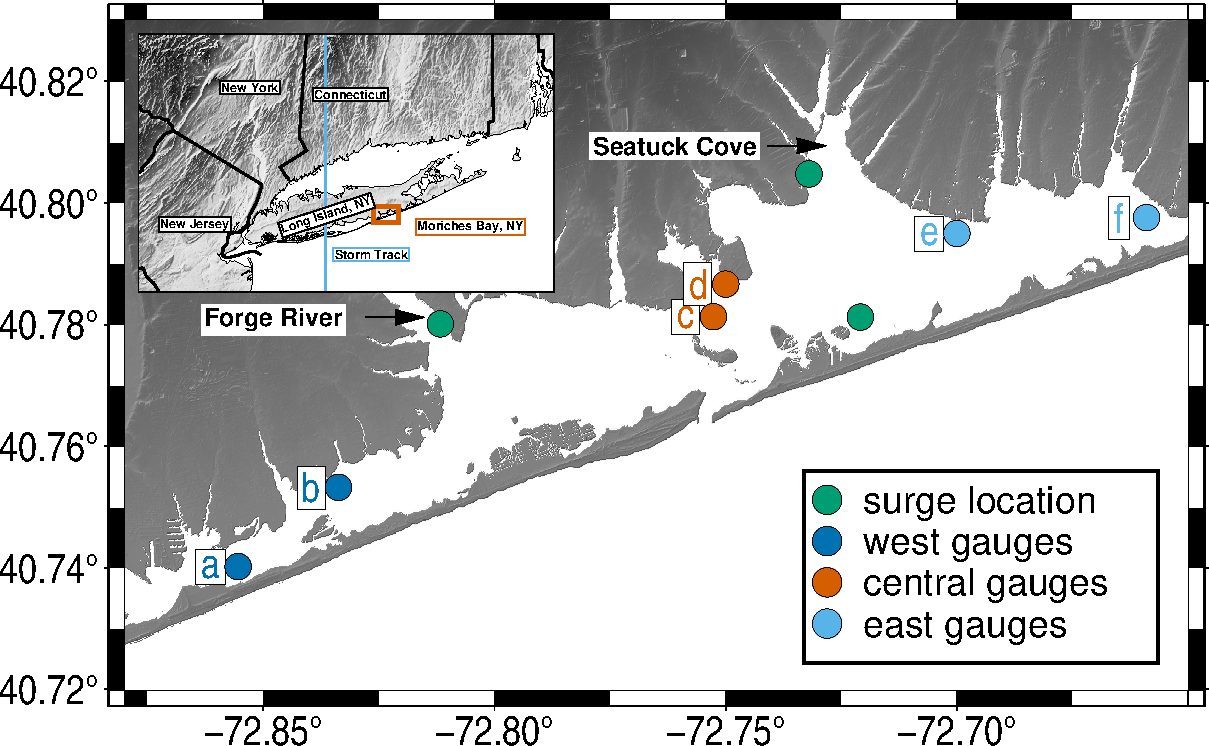
\includegraphics[width=0.95\textwidth]{figures/fig2_v2.pdf}
    \caption{Map of study area Moriches, NY. Green circles are locations of surge measurements. Circles with letters indicate locations of synthetic tide gauges shown in figure \ref{fig:2}}
    \label{fig:2}
\end{figure}

\section{Results}

 Figure~\ref{fig:3} illustrates the surge heights for each category of simulation. The mean of the surge height is higher for the \emph{Location} simulations with the density peak at 1.75 meters, 1.70 meters, and 1.43 meters for west, central, east bay respectively. The variance is also large at 0.05 m$^2$, 0.024 m$^2$, 0.03 m$^2$ as compared to the other simulations. When constrained by a maximum of six breaches the depth variations have the largest surge height mean at 1.06 m, 1.07 m, 0.84 m. The width scenarios mean surge height is 0.97 m, 1.09 m, 0.78 m and the width/depth/number of breaches simulations have a mean surge height of 0.88 m, 0.98 m, 0.72 m. The width scenarios have a larger variance of 0.004 m$^2$, 0.004 m$^2$, 0.002 m$^2$ as compared to depth 0.003 m$^2$, 0.0003 m$^2$, 0.005 m$^2$ or both 0.006 m$^2$, 0.002 m$^2$, 0.002 m$^2$. 

\begin{figure}[ht]
    \centering
    \resizebox{\textwidth}{!}{%
            %% Creator: Matplotlib, PGF backend
%%
%% To include the figure in your LaTeX document, write
%%   \input{<filename>.pgf}
%%
%% Make sure the required packages are loaded in your preamble
%%   \usepackage{pgf}
%%
%% Also ensure that all the required font packages are loaded; for instance,
%% the lmodern package is sometimes necessary when using math font.
%%   \usepackage{lmodern}
%%
%% Figures using additional raster images can only be included by \input if
%% they are in the same directory as the main LaTeX file. For loading figures
%% from other directories you can use the `import` package
%%   \usepackage{import}
%%
%% and then include the figures with
%%   \import{<path to file>}{<filename>.pgf}
%%
%% Matplotlib used the following preamble
%%   \usepackage{fontspec}
%%   \setmainfont{DejaVuSerif.ttf}[Path=\detokenize{/home/catherinej/miniconda3/envs/claw/lib/python3.10/site-packages/matplotlib/mpl-data/fonts/ttf/}]
%%   \setsansfont{helvetica.ttf}[Path=\detokenize{/home/catherinej/miniconda3/envs/claw/lib/python3.10/site-packages/matplotlib/mpl-data/fonts/ttf/}]
%%   \setmonofont{DejaVuSansMono.ttf}[Path=\detokenize{/home/catherinej/miniconda3/envs/claw/lib/python3.10/site-packages/matplotlib/mpl-data/fonts/ttf/}]
%%
\begingroup%
\makeatletter%
\begin{pgfpicture}%
\pgfpathrectangle{\pgfpointorigin}{\pgfqpoint{9.008044in}{3.188875in}}%
\pgfusepath{use as bounding box, clip}%
\begin{pgfscope}%
\pgfsetbuttcap%
\pgfsetmiterjoin%
\definecolor{currentfill}{rgb}{1.000000,1.000000,1.000000}%
\pgfsetfillcolor{currentfill}%
\pgfsetlinewidth{0.000000pt}%
\definecolor{currentstroke}{rgb}{1.000000,1.000000,1.000000}%
\pgfsetstrokecolor{currentstroke}%
\pgfsetdash{}{0pt}%
\pgfpathmoveto{\pgfqpoint{0.000000in}{0.000000in}}%
\pgfpathlineto{\pgfqpoint{9.008044in}{0.000000in}}%
\pgfpathlineto{\pgfqpoint{9.008044in}{3.188875in}}%
\pgfpathlineto{\pgfqpoint{0.000000in}{3.188875in}}%
\pgfpathlineto{\pgfqpoint{0.000000in}{0.000000in}}%
\pgfpathclose%
\pgfusepath{fill}%
\end{pgfscope}%
\begin{pgfscope}%
\pgfsetbuttcap%
\pgfsetmiterjoin%
\definecolor{currentfill}{rgb}{1.000000,1.000000,1.000000}%
\pgfsetfillcolor{currentfill}%
\pgfsetlinewidth{0.000000pt}%
\definecolor{currentstroke}{rgb}{0.000000,0.000000,0.000000}%
\pgfsetstrokecolor{currentstroke}%
\pgfsetstrokeopacity{0.000000}%
\pgfsetdash{}{0pt}%
\pgfpathmoveto{\pgfqpoint{0.853515in}{0.656145in}}%
\pgfpathlineto{\pgfqpoint{3.132927in}{0.656145in}}%
\pgfpathlineto{\pgfqpoint{3.132927in}{2.846145in}}%
\pgfpathlineto{\pgfqpoint{0.853515in}{2.846145in}}%
\pgfpathlineto{\pgfqpoint{0.853515in}{0.656145in}}%
\pgfpathclose%
\pgfusepath{fill}%
\end{pgfscope}%
\begin{pgfscope}%
\pgfpathrectangle{\pgfqpoint{0.853515in}{0.656145in}}{\pgfqpoint{2.279412in}{2.190000in}}%
\pgfusepath{clip}%
\pgfsetbuttcap%
\pgfsetmiterjoin%
\definecolor{currentfill}{rgb}{0.835294,0.368627,0.000000}%
\pgfsetfillcolor{currentfill}%
\pgfsetfillopacity{0.200000}%
\pgfsetlinewidth{0.803000pt}%
\definecolor{currentstroke}{rgb}{0.000000,0.000000,0.000000}%
\pgfsetstrokecolor{currentstroke}%
\pgfsetstrokeopacity{0.200000}%
\pgfsetdash{}{0pt}%
\pgfpathmoveto{\pgfqpoint{1.160962in}{0.656145in}}%
\pgfpathlineto{\pgfqpoint{1.160962in}{1.301347in}}%
\pgfpathlineto{\pgfqpoint{1.256110in}{1.301347in}}%
\pgfpathlineto{\pgfqpoint{1.256110in}{1.144655in}}%
\pgfpathlineto{\pgfqpoint{1.351258in}{1.144655in}}%
\pgfpathlineto{\pgfqpoint{1.351258in}{1.421170in}}%
\pgfpathlineto{\pgfqpoint{1.446405in}{1.421170in}}%
\pgfpathlineto{\pgfqpoint{1.446405in}{1.172307in}}%
\pgfpathlineto{\pgfqpoint{1.541553in}{1.172307in}}%
\pgfpathlineto{\pgfqpoint{1.541553in}{0.951095in}}%
\pgfpathlineto{\pgfqpoint{1.636701in}{0.951095in}}%
\pgfpathlineto{\pgfqpoint{1.636701in}{0.683797in}}%
\pgfpathlineto{\pgfqpoint{1.731849in}{0.683797in}}%
\pgfpathlineto{\pgfqpoint{1.731849in}{0.656145in}}%
\pgfpathlineto{\pgfqpoint{1.826996in}{0.656145in}}%
\pgfpathlineto{\pgfqpoint{1.826996in}{0.656145in}}%
\pgfpathlineto{\pgfqpoint{1.922144in}{0.656145in}}%
\pgfpathlineto{\pgfqpoint{1.922144in}{0.656145in}}%
\pgfpathlineto{\pgfqpoint{2.017292in}{0.656145in}}%
\pgfpathlineto{\pgfqpoint{2.017292in}{0.656145in}}%
\pgfpathlineto{\pgfqpoint{2.112440in}{0.656145in}}%
\pgfpathlineto{\pgfqpoint{2.112440in}{0.656145in}}%
\pgfpathlineto{\pgfqpoint{2.207587in}{0.656145in}}%
\pgfpathlineto{\pgfqpoint{2.207587in}{0.656145in}}%
\pgfpathlineto{\pgfqpoint{2.302735in}{0.656145in}}%
\pgfpathlineto{\pgfqpoint{2.302735in}{0.656145in}}%
\pgfpathlineto{\pgfqpoint{2.397883in}{0.656145in}}%
\pgfpathlineto{\pgfqpoint{2.397883in}{0.656145in}}%
\pgfpathlineto{\pgfqpoint{2.493031in}{0.656145in}}%
\pgfpathlineto{\pgfqpoint{2.493031in}{0.656145in}}%
\pgfpathlineto{\pgfqpoint{2.588178in}{0.656145in}}%
\pgfpathlineto{\pgfqpoint{2.588178in}{0.656145in}}%
\pgfpathlineto{\pgfqpoint{2.683326in}{0.656145in}}%
\pgfpathlineto{\pgfqpoint{2.683326in}{0.656145in}}%
\pgfpathlineto{\pgfqpoint{2.778474in}{0.656145in}}%
\pgfpathlineto{\pgfqpoint{2.778474in}{0.656145in}}%
\pgfpathlineto{\pgfqpoint{2.873622in}{0.656145in}}%
\pgfpathlineto{\pgfqpoint{2.873622in}{0.656145in}}%
\pgfpathlineto{\pgfqpoint{2.968769in}{0.656145in}}%
\pgfpathlineto{\pgfqpoint{2.968769in}{0.656145in}}%
\pgfpathlineto{\pgfqpoint{3.063917in}{0.656145in}}%
\pgfpathlineto{\pgfqpoint{3.063917in}{0.656145in}}%
\pgfpathlineto{\pgfqpoint{2.968769in}{0.656145in}}%
\pgfpathlineto{\pgfqpoint{2.968769in}{0.656145in}}%
\pgfpathlineto{\pgfqpoint{2.873622in}{0.656145in}}%
\pgfpathlineto{\pgfqpoint{2.873622in}{0.656145in}}%
\pgfpathlineto{\pgfqpoint{2.778474in}{0.656145in}}%
\pgfpathlineto{\pgfqpoint{2.778474in}{0.656145in}}%
\pgfpathlineto{\pgfqpoint{2.683326in}{0.656145in}}%
\pgfpathlineto{\pgfqpoint{2.683326in}{0.656145in}}%
\pgfpathlineto{\pgfqpoint{2.588178in}{0.656145in}}%
\pgfpathlineto{\pgfqpoint{2.588178in}{0.656145in}}%
\pgfpathlineto{\pgfqpoint{2.493031in}{0.656145in}}%
\pgfpathlineto{\pgfqpoint{2.493031in}{0.656145in}}%
\pgfpathlineto{\pgfqpoint{2.397883in}{0.656145in}}%
\pgfpathlineto{\pgfqpoint{2.397883in}{0.656145in}}%
\pgfpathlineto{\pgfqpoint{2.302735in}{0.656145in}}%
\pgfpathlineto{\pgfqpoint{2.302735in}{0.656145in}}%
\pgfpathlineto{\pgfqpoint{2.207587in}{0.656145in}}%
\pgfpathlineto{\pgfqpoint{2.207587in}{0.656145in}}%
\pgfpathlineto{\pgfqpoint{2.112440in}{0.656145in}}%
\pgfpathlineto{\pgfqpoint{2.112440in}{0.656145in}}%
\pgfpathlineto{\pgfqpoint{2.017292in}{0.656145in}}%
\pgfpathlineto{\pgfqpoint{2.017292in}{0.656145in}}%
\pgfpathlineto{\pgfqpoint{1.922144in}{0.656145in}}%
\pgfpathlineto{\pgfqpoint{1.922144in}{0.656145in}}%
\pgfpathlineto{\pgfqpoint{1.826996in}{0.656145in}}%
\pgfpathlineto{\pgfqpoint{1.826996in}{0.656145in}}%
\pgfpathlineto{\pgfqpoint{1.731849in}{0.656145in}}%
\pgfpathlineto{\pgfqpoint{1.731849in}{0.656145in}}%
\pgfpathlineto{\pgfqpoint{1.636701in}{0.656145in}}%
\pgfpathlineto{\pgfqpoint{1.636701in}{0.656145in}}%
\pgfpathlineto{\pgfqpoint{1.541553in}{0.656145in}}%
\pgfpathlineto{\pgfqpoint{1.541553in}{0.656145in}}%
\pgfpathlineto{\pgfqpoint{1.446405in}{0.656145in}}%
\pgfpathlineto{\pgfqpoint{1.446405in}{0.656145in}}%
\pgfpathlineto{\pgfqpoint{1.351258in}{0.656145in}}%
\pgfpathlineto{\pgfqpoint{1.351258in}{0.656145in}}%
\pgfpathlineto{\pgfqpoint{1.256110in}{0.656145in}}%
\pgfpathlineto{\pgfqpoint{1.256110in}{0.656145in}}%
\pgfpathlineto{\pgfqpoint{1.160962in}{0.656145in}}%
\pgfpathclose%
\pgfusepath{stroke,fill}%
\end{pgfscope}%
\begin{pgfscope}%
\pgfpathrectangle{\pgfqpoint{0.853515in}{0.656145in}}{\pgfqpoint{2.279412in}{2.190000in}}%
\pgfusepath{clip}%
\pgfsetbuttcap%
\pgfsetmiterjoin%
\definecolor{currentfill}{rgb}{0.000000,0.619608,0.450980}%
\pgfsetfillcolor{currentfill}%
\pgfsetfillopacity{0.200000}%
\pgfsetlinewidth{0.803000pt}%
\definecolor{currentstroke}{rgb}{0.000000,0.000000,0.000000}%
\pgfsetstrokecolor{currentstroke}%
\pgfsetstrokeopacity{0.200000}%
\pgfsetdash{}{0pt}%
\pgfpathmoveto{\pgfqpoint{1.160962in}{0.656145in}}%
\pgfpathlineto{\pgfqpoint{1.160962in}{0.656145in}}%
\pgfpathlineto{\pgfqpoint{1.256110in}{0.656145in}}%
\pgfpathlineto{\pgfqpoint{1.256110in}{0.738742in}}%
\pgfpathlineto{\pgfqpoint{1.351258in}{0.738742in}}%
\pgfpathlineto{\pgfqpoint{1.351258in}{1.375919in}}%
\pgfpathlineto{\pgfqpoint{1.446405in}{1.375919in}}%
\pgfpathlineto{\pgfqpoint{1.446405in}{1.576512in}}%
\pgfpathlineto{\pgfqpoint{1.541553in}{1.576512in}}%
\pgfpathlineto{\pgfqpoint{1.541553in}{1.110429in}}%
\pgfpathlineto{\pgfqpoint{1.636701in}{1.110429in}}%
\pgfpathlineto{\pgfqpoint{1.636701in}{1.163527in}}%
\pgfpathlineto{\pgfqpoint{1.731849in}{1.163527in}}%
\pgfpathlineto{\pgfqpoint{1.731849in}{0.709243in}}%
\pgfpathlineto{\pgfqpoint{1.826996in}{0.709243in}}%
\pgfpathlineto{\pgfqpoint{1.826996in}{0.656145in}}%
\pgfpathlineto{\pgfqpoint{1.922144in}{0.656145in}}%
\pgfpathlineto{\pgfqpoint{1.922144in}{0.656145in}}%
\pgfpathlineto{\pgfqpoint{2.017292in}{0.656145in}}%
\pgfpathlineto{\pgfqpoint{2.017292in}{0.656145in}}%
\pgfpathlineto{\pgfqpoint{2.112440in}{0.656145in}}%
\pgfpathlineto{\pgfqpoint{2.112440in}{0.656145in}}%
\pgfpathlineto{\pgfqpoint{2.207587in}{0.656145in}}%
\pgfpathlineto{\pgfqpoint{2.207587in}{0.656145in}}%
\pgfpathlineto{\pgfqpoint{2.302735in}{0.656145in}}%
\pgfpathlineto{\pgfqpoint{2.302735in}{0.656145in}}%
\pgfpathlineto{\pgfqpoint{2.397883in}{0.656145in}}%
\pgfpathlineto{\pgfqpoint{2.397883in}{0.656145in}}%
\pgfpathlineto{\pgfqpoint{2.493031in}{0.656145in}}%
\pgfpathlineto{\pgfqpoint{2.493031in}{0.656145in}}%
\pgfpathlineto{\pgfqpoint{2.588178in}{0.656145in}}%
\pgfpathlineto{\pgfqpoint{2.588178in}{0.656145in}}%
\pgfpathlineto{\pgfqpoint{2.683326in}{0.656145in}}%
\pgfpathlineto{\pgfqpoint{2.683326in}{0.656145in}}%
\pgfpathlineto{\pgfqpoint{2.778474in}{0.656145in}}%
\pgfpathlineto{\pgfqpoint{2.778474in}{0.656145in}}%
\pgfpathlineto{\pgfqpoint{2.873622in}{0.656145in}}%
\pgfpathlineto{\pgfqpoint{2.873622in}{0.656145in}}%
\pgfpathlineto{\pgfqpoint{2.968769in}{0.656145in}}%
\pgfpathlineto{\pgfqpoint{2.968769in}{0.656145in}}%
\pgfpathlineto{\pgfqpoint{3.063917in}{0.656145in}}%
\pgfpathlineto{\pgfqpoint{3.063917in}{0.656145in}}%
\pgfpathlineto{\pgfqpoint{2.968769in}{0.656145in}}%
\pgfpathlineto{\pgfqpoint{2.968769in}{0.656145in}}%
\pgfpathlineto{\pgfqpoint{2.873622in}{0.656145in}}%
\pgfpathlineto{\pgfqpoint{2.873622in}{0.656145in}}%
\pgfpathlineto{\pgfqpoint{2.778474in}{0.656145in}}%
\pgfpathlineto{\pgfqpoint{2.778474in}{0.656145in}}%
\pgfpathlineto{\pgfqpoint{2.683326in}{0.656145in}}%
\pgfpathlineto{\pgfqpoint{2.683326in}{0.656145in}}%
\pgfpathlineto{\pgfqpoint{2.588178in}{0.656145in}}%
\pgfpathlineto{\pgfqpoint{2.588178in}{0.656145in}}%
\pgfpathlineto{\pgfqpoint{2.493031in}{0.656145in}}%
\pgfpathlineto{\pgfqpoint{2.493031in}{0.656145in}}%
\pgfpathlineto{\pgfqpoint{2.397883in}{0.656145in}}%
\pgfpathlineto{\pgfqpoint{2.397883in}{0.656145in}}%
\pgfpathlineto{\pgfqpoint{2.302735in}{0.656145in}}%
\pgfpathlineto{\pgfqpoint{2.302735in}{0.656145in}}%
\pgfpathlineto{\pgfqpoint{2.207587in}{0.656145in}}%
\pgfpathlineto{\pgfqpoint{2.207587in}{0.656145in}}%
\pgfpathlineto{\pgfqpoint{2.112440in}{0.656145in}}%
\pgfpathlineto{\pgfqpoint{2.112440in}{0.656145in}}%
\pgfpathlineto{\pgfqpoint{2.017292in}{0.656145in}}%
\pgfpathlineto{\pgfqpoint{2.017292in}{0.656145in}}%
\pgfpathlineto{\pgfqpoint{1.922144in}{0.656145in}}%
\pgfpathlineto{\pgfqpoint{1.922144in}{0.656145in}}%
\pgfpathlineto{\pgfqpoint{1.826996in}{0.656145in}}%
\pgfpathlineto{\pgfqpoint{1.826996in}{0.656145in}}%
\pgfpathlineto{\pgfqpoint{1.731849in}{0.656145in}}%
\pgfpathlineto{\pgfqpoint{1.731849in}{0.656145in}}%
\pgfpathlineto{\pgfqpoint{1.636701in}{0.656145in}}%
\pgfpathlineto{\pgfqpoint{1.636701in}{0.656145in}}%
\pgfpathlineto{\pgfqpoint{1.541553in}{0.656145in}}%
\pgfpathlineto{\pgfqpoint{1.541553in}{0.656145in}}%
\pgfpathlineto{\pgfqpoint{1.446405in}{0.656145in}}%
\pgfpathlineto{\pgfqpoint{1.446405in}{0.656145in}}%
\pgfpathlineto{\pgfqpoint{1.351258in}{0.656145in}}%
\pgfpathlineto{\pgfqpoint{1.351258in}{0.656145in}}%
\pgfpathlineto{\pgfqpoint{1.256110in}{0.656145in}}%
\pgfpathlineto{\pgfqpoint{1.256110in}{0.656145in}}%
\pgfpathlineto{\pgfqpoint{1.160962in}{0.656145in}}%
\pgfpathclose%
\pgfusepath{stroke,fill}%
\end{pgfscope}%
\begin{pgfscope}%
\pgfpathrectangle{\pgfqpoint{0.853515in}{0.656145in}}{\pgfqpoint{2.279412in}{2.190000in}}%
\pgfusepath{clip}%
\pgfsetbuttcap%
\pgfsetmiterjoin%
\definecolor{currentfill}{rgb}{0.337255,0.705882,0.913725}%
\pgfsetfillcolor{currentfill}%
\pgfsetfillopacity{0.200000}%
\pgfsetlinewidth{0.803000pt}%
\definecolor{currentstroke}{rgb}{0.000000,0.000000,0.000000}%
\pgfsetstrokecolor{currentstroke}%
\pgfsetstrokeopacity{0.200000}%
\pgfsetdash{}{0pt}%
\pgfpathmoveto{\pgfqpoint{1.160962in}{0.656145in}}%
\pgfpathlineto{\pgfqpoint{1.160962in}{0.656145in}}%
\pgfpathlineto{\pgfqpoint{1.256110in}{0.656145in}}%
\pgfpathlineto{\pgfqpoint{1.256110in}{0.656145in}}%
\pgfpathlineto{\pgfqpoint{1.351258in}{0.656145in}}%
\pgfpathlineto{\pgfqpoint{1.351258in}{0.656145in}}%
\pgfpathlineto{\pgfqpoint{1.446405in}{0.656145in}}%
\pgfpathlineto{\pgfqpoint{1.446405in}{0.740078in}}%
\pgfpathlineto{\pgfqpoint{1.541553in}{0.740078in}}%
\pgfpathlineto{\pgfqpoint{1.541553in}{1.411540in}}%
\pgfpathlineto{\pgfqpoint{1.636701in}{1.411540in}}%
\pgfpathlineto{\pgfqpoint{1.636701in}{2.483297in}}%
\pgfpathlineto{\pgfqpoint{1.731849in}{2.483297in}}%
\pgfpathlineto{\pgfqpoint{1.731849in}{0.727165in}}%
\pgfpathlineto{\pgfqpoint{1.826996in}{0.727165in}}%
\pgfpathlineto{\pgfqpoint{1.826996in}{0.656145in}}%
\pgfpathlineto{\pgfqpoint{1.922144in}{0.656145in}}%
\pgfpathlineto{\pgfqpoint{1.922144in}{0.656145in}}%
\pgfpathlineto{\pgfqpoint{2.017292in}{0.656145in}}%
\pgfpathlineto{\pgfqpoint{2.017292in}{0.656145in}}%
\pgfpathlineto{\pgfqpoint{2.112440in}{0.656145in}}%
\pgfpathlineto{\pgfqpoint{2.112440in}{0.656145in}}%
\pgfpathlineto{\pgfqpoint{2.207587in}{0.656145in}}%
\pgfpathlineto{\pgfqpoint{2.207587in}{0.656145in}}%
\pgfpathlineto{\pgfqpoint{2.302735in}{0.656145in}}%
\pgfpathlineto{\pgfqpoint{2.302735in}{0.656145in}}%
\pgfpathlineto{\pgfqpoint{2.397883in}{0.656145in}}%
\pgfpathlineto{\pgfqpoint{2.397883in}{0.656145in}}%
\pgfpathlineto{\pgfqpoint{2.493031in}{0.656145in}}%
\pgfpathlineto{\pgfqpoint{2.493031in}{0.656145in}}%
\pgfpathlineto{\pgfqpoint{2.588178in}{0.656145in}}%
\pgfpathlineto{\pgfqpoint{2.588178in}{0.656145in}}%
\pgfpathlineto{\pgfqpoint{2.683326in}{0.656145in}}%
\pgfpathlineto{\pgfqpoint{2.683326in}{0.656145in}}%
\pgfpathlineto{\pgfqpoint{2.778474in}{0.656145in}}%
\pgfpathlineto{\pgfqpoint{2.778474in}{0.656145in}}%
\pgfpathlineto{\pgfqpoint{2.873622in}{0.656145in}}%
\pgfpathlineto{\pgfqpoint{2.873622in}{0.656145in}}%
\pgfpathlineto{\pgfqpoint{2.968769in}{0.656145in}}%
\pgfpathlineto{\pgfqpoint{2.968769in}{0.656145in}}%
\pgfpathlineto{\pgfqpoint{3.063917in}{0.656145in}}%
\pgfpathlineto{\pgfqpoint{3.063917in}{0.656145in}}%
\pgfpathlineto{\pgfqpoint{2.968769in}{0.656145in}}%
\pgfpathlineto{\pgfqpoint{2.968769in}{0.656145in}}%
\pgfpathlineto{\pgfqpoint{2.873622in}{0.656145in}}%
\pgfpathlineto{\pgfqpoint{2.873622in}{0.656145in}}%
\pgfpathlineto{\pgfqpoint{2.778474in}{0.656145in}}%
\pgfpathlineto{\pgfqpoint{2.778474in}{0.656145in}}%
\pgfpathlineto{\pgfqpoint{2.683326in}{0.656145in}}%
\pgfpathlineto{\pgfqpoint{2.683326in}{0.656145in}}%
\pgfpathlineto{\pgfqpoint{2.588178in}{0.656145in}}%
\pgfpathlineto{\pgfqpoint{2.588178in}{0.656145in}}%
\pgfpathlineto{\pgfqpoint{2.493031in}{0.656145in}}%
\pgfpathlineto{\pgfqpoint{2.493031in}{0.656145in}}%
\pgfpathlineto{\pgfqpoint{2.397883in}{0.656145in}}%
\pgfpathlineto{\pgfqpoint{2.397883in}{0.656145in}}%
\pgfpathlineto{\pgfqpoint{2.302735in}{0.656145in}}%
\pgfpathlineto{\pgfqpoint{2.302735in}{0.656145in}}%
\pgfpathlineto{\pgfqpoint{2.207587in}{0.656145in}}%
\pgfpathlineto{\pgfqpoint{2.207587in}{0.656145in}}%
\pgfpathlineto{\pgfqpoint{2.112440in}{0.656145in}}%
\pgfpathlineto{\pgfqpoint{2.112440in}{0.656145in}}%
\pgfpathlineto{\pgfqpoint{2.017292in}{0.656145in}}%
\pgfpathlineto{\pgfqpoint{2.017292in}{0.656145in}}%
\pgfpathlineto{\pgfqpoint{1.922144in}{0.656145in}}%
\pgfpathlineto{\pgfqpoint{1.922144in}{0.656145in}}%
\pgfpathlineto{\pgfqpoint{1.826996in}{0.656145in}}%
\pgfpathlineto{\pgfqpoint{1.826996in}{0.656145in}}%
\pgfpathlineto{\pgfqpoint{1.731849in}{0.656145in}}%
\pgfpathlineto{\pgfqpoint{1.731849in}{0.656145in}}%
\pgfpathlineto{\pgfqpoint{1.636701in}{0.656145in}}%
\pgfpathlineto{\pgfqpoint{1.636701in}{0.656145in}}%
\pgfpathlineto{\pgfqpoint{1.541553in}{0.656145in}}%
\pgfpathlineto{\pgfqpoint{1.541553in}{0.656145in}}%
\pgfpathlineto{\pgfqpoint{1.446405in}{0.656145in}}%
\pgfpathlineto{\pgfqpoint{1.446405in}{0.656145in}}%
\pgfpathlineto{\pgfqpoint{1.351258in}{0.656145in}}%
\pgfpathlineto{\pgfqpoint{1.351258in}{0.656145in}}%
\pgfpathlineto{\pgfqpoint{1.256110in}{0.656145in}}%
\pgfpathlineto{\pgfqpoint{1.256110in}{0.656145in}}%
\pgfpathlineto{\pgfqpoint{1.160962in}{0.656145in}}%
\pgfpathclose%
\pgfusepath{stroke,fill}%
\end{pgfscope}%
\begin{pgfscope}%
\pgfpathrectangle{\pgfqpoint{0.853515in}{0.656145in}}{\pgfqpoint{2.279412in}{2.190000in}}%
\pgfusepath{clip}%
\pgfsetbuttcap%
\pgfsetmiterjoin%
\definecolor{currentfill}{rgb}{0.800000,0.474510,0.654902}%
\pgfsetfillcolor{currentfill}%
\pgfsetfillopacity{0.200000}%
\pgfsetlinewidth{0.803000pt}%
\definecolor{currentstroke}{rgb}{0.000000,0.000000,0.000000}%
\pgfsetstrokecolor{currentstroke}%
\pgfsetstrokeopacity{0.200000}%
\pgfsetdash{}{0pt}%
\pgfpathmoveto{\pgfqpoint{1.160962in}{0.656145in}}%
\pgfpathlineto{\pgfqpoint{1.160962in}{0.716979in}}%
\pgfpathlineto{\pgfqpoint{1.256110in}{0.716979in}}%
\pgfpathlineto{\pgfqpoint{1.256110in}{0.716979in}}%
\pgfpathlineto{\pgfqpoint{1.351258in}{0.716979in}}%
\pgfpathlineto{\pgfqpoint{1.351258in}{0.708288in}}%
\pgfpathlineto{\pgfqpoint{1.446405in}{0.708288in}}%
\pgfpathlineto{\pgfqpoint{1.446405in}{0.682217in}}%
\pgfpathlineto{\pgfqpoint{1.541553in}{0.682217in}}%
\pgfpathlineto{\pgfqpoint{1.541553in}{0.734359in}}%
\pgfpathlineto{\pgfqpoint{1.636701in}{0.734359in}}%
\pgfpathlineto{\pgfqpoint{1.636701in}{0.664836in}}%
\pgfpathlineto{\pgfqpoint{1.731849in}{0.664836in}}%
\pgfpathlineto{\pgfqpoint{1.731849in}{0.716979in}}%
\pgfpathlineto{\pgfqpoint{1.826996in}{0.716979in}}%
\pgfpathlineto{\pgfqpoint{1.826996in}{0.725669in}}%
\pgfpathlineto{\pgfqpoint{1.922144in}{0.725669in}}%
\pgfpathlineto{\pgfqpoint{1.922144in}{0.725669in}}%
\pgfpathlineto{\pgfqpoint{2.017292in}{0.725669in}}%
\pgfpathlineto{\pgfqpoint{2.017292in}{0.725669in}}%
\pgfpathlineto{\pgfqpoint{2.112440in}{0.725669in}}%
\pgfpathlineto{\pgfqpoint{2.112440in}{0.786502in}}%
\pgfpathlineto{\pgfqpoint{2.207587in}{0.786502in}}%
\pgfpathlineto{\pgfqpoint{2.207587in}{0.769121in}}%
\pgfpathlineto{\pgfqpoint{2.302735in}{0.769121in}}%
\pgfpathlineto{\pgfqpoint{2.302735in}{0.829955in}}%
\pgfpathlineto{\pgfqpoint{2.397883in}{0.829955in}}%
\pgfpathlineto{\pgfqpoint{2.397883in}{0.777812in}}%
\pgfpathlineto{\pgfqpoint{2.493031in}{0.777812in}}%
\pgfpathlineto{\pgfqpoint{2.493031in}{0.838645in}}%
\pgfpathlineto{\pgfqpoint{2.588178in}{0.838645in}}%
\pgfpathlineto{\pgfqpoint{2.588178in}{0.812574in}}%
\pgfpathlineto{\pgfqpoint{2.683326in}{0.812574in}}%
\pgfpathlineto{\pgfqpoint{2.683326in}{0.795193in}}%
\pgfpathlineto{\pgfqpoint{2.778474in}{0.795193in}}%
\pgfpathlineto{\pgfqpoint{2.778474in}{0.856026in}}%
\pgfpathlineto{\pgfqpoint{2.873622in}{0.856026in}}%
\pgfpathlineto{\pgfqpoint{2.873622in}{1.203645in}}%
\pgfpathlineto{\pgfqpoint{2.968769in}{1.203645in}}%
\pgfpathlineto{\pgfqpoint{2.968769in}{1.073288in}}%
\pgfpathlineto{\pgfqpoint{3.063917in}{1.073288in}}%
\pgfpathlineto{\pgfqpoint{3.063917in}{0.656145in}}%
\pgfpathlineto{\pgfqpoint{2.968769in}{0.656145in}}%
\pgfpathlineto{\pgfqpoint{2.968769in}{0.656145in}}%
\pgfpathlineto{\pgfqpoint{2.873622in}{0.656145in}}%
\pgfpathlineto{\pgfqpoint{2.873622in}{0.656145in}}%
\pgfpathlineto{\pgfqpoint{2.778474in}{0.656145in}}%
\pgfpathlineto{\pgfqpoint{2.778474in}{0.656145in}}%
\pgfpathlineto{\pgfqpoint{2.683326in}{0.656145in}}%
\pgfpathlineto{\pgfqpoint{2.683326in}{0.656145in}}%
\pgfpathlineto{\pgfqpoint{2.588178in}{0.656145in}}%
\pgfpathlineto{\pgfqpoint{2.588178in}{0.656145in}}%
\pgfpathlineto{\pgfqpoint{2.493031in}{0.656145in}}%
\pgfpathlineto{\pgfqpoint{2.493031in}{0.656145in}}%
\pgfpathlineto{\pgfqpoint{2.397883in}{0.656145in}}%
\pgfpathlineto{\pgfqpoint{2.397883in}{0.656145in}}%
\pgfpathlineto{\pgfqpoint{2.302735in}{0.656145in}}%
\pgfpathlineto{\pgfqpoint{2.302735in}{0.656145in}}%
\pgfpathlineto{\pgfqpoint{2.207587in}{0.656145in}}%
\pgfpathlineto{\pgfqpoint{2.207587in}{0.656145in}}%
\pgfpathlineto{\pgfqpoint{2.112440in}{0.656145in}}%
\pgfpathlineto{\pgfqpoint{2.112440in}{0.656145in}}%
\pgfpathlineto{\pgfqpoint{2.017292in}{0.656145in}}%
\pgfpathlineto{\pgfqpoint{2.017292in}{0.656145in}}%
\pgfpathlineto{\pgfqpoint{1.922144in}{0.656145in}}%
\pgfpathlineto{\pgfqpoint{1.922144in}{0.656145in}}%
\pgfpathlineto{\pgfqpoint{1.826996in}{0.656145in}}%
\pgfpathlineto{\pgfqpoint{1.826996in}{0.656145in}}%
\pgfpathlineto{\pgfqpoint{1.731849in}{0.656145in}}%
\pgfpathlineto{\pgfqpoint{1.731849in}{0.656145in}}%
\pgfpathlineto{\pgfqpoint{1.636701in}{0.656145in}}%
\pgfpathlineto{\pgfqpoint{1.636701in}{0.656145in}}%
\pgfpathlineto{\pgfqpoint{1.541553in}{0.656145in}}%
\pgfpathlineto{\pgfqpoint{1.541553in}{0.656145in}}%
\pgfpathlineto{\pgfqpoint{1.446405in}{0.656145in}}%
\pgfpathlineto{\pgfqpoint{1.446405in}{0.656145in}}%
\pgfpathlineto{\pgfqpoint{1.351258in}{0.656145in}}%
\pgfpathlineto{\pgfqpoint{1.351258in}{0.656145in}}%
\pgfpathlineto{\pgfqpoint{1.256110in}{0.656145in}}%
\pgfpathlineto{\pgfqpoint{1.256110in}{0.656145in}}%
\pgfpathlineto{\pgfqpoint{1.160962in}{0.656145in}}%
\pgfpathclose%
\pgfusepath{stroke,fill}%
\end{pgfscope}%
\begin{pgfscope}%
\pgfsetbuttcap%
\pgfsetroundjoin%
\definecolor{currentfill}{rgb}{0.196078,0.188235,0.203922}%
\pgfsetfillcolor{currentfill}%
\pgfsetlinewidth{0.803000pt}%
\definecolor{currentstroke}{rgb}{0.196078,0.188235,0.203922}%
\pgfsetstrokecolor{currentstroke}%
\pgfsetdash{}{0pt}%
\pgfsys@defobject{currentmarker}{\pgfqpoint{0.000000in}{-0.048611in}}{\pgfqpoint{0.000000in}{0.000000in}}{%
\pgfpathmoveto{\pgfqpoint{0.000000in}{0.000000in}}%
\pgfpathlineto{\pgfqpoint{0.000000in}{-0.048611in}}%
\pgfusepath{stroke,fill}%
}%
\begin{pgfscope}%
\pgfsys@transformshift{0.853515in}{0.656145in}%
\pgfsys@useobject{currentmarker}{}%
\end{pgfscope}%
\end{pgfscope}%
\begin{pgfscope}%
\definecolor{textcolor}{rgb}{0.196078,0.188235,0.203922}%
\pgfsetstrokecolor{textcolor}%
\pgfsetfillcolor{textcolor}%
\pgftext[x=0.853515in,y=0.558923in,,top]{\color{textcolor}\sffamily\fontsize{10.000000}{12.000000}\selectfont 0.55}%
\end{pgfscope}%
\begin{pgfscope}%
\pgfsetbuttcap%
\pgfsetroundjoin%
\definecolor{currentfill}{rgb}{0.196078,0.188235,0.203922}%
\pgfsetfillcolor{currentfill}%
\pgfsetlinewidth{0.803000pt}%
\definecolor{currentstroke}{rgb}{0.196078,0.188235,0.203922}%
\pgfsetstrokecolor{currentstroke}%
\pgfsetdash{}{0pt}%
\pgfsys@defobject{currentmarker}{\pgfqpoint{0.000000in}{-0.048611in}}{\pgfqpoint{0.000000in}{0.000000in}}{%
\pgfpathmoveto{\pgfqpoint{0.000000in}{0.000000in}}%
\pgfpathlineto{\pgfqpoint{0.000000in}{-0.048611in}}%
\pgfusepath{stroke,fill}%
}%
\begin{pgfscope}%
\pgfsys@transformshift{1.179146in}{0.656145in}%
\pgfsys@useobject{currentmarker}{}%
\end{pgfscope}%
\end{pgfscope}%
\begin{pgfscope}%
\definecolor{textcolor}{rgb}{0.196078,0.188235,0.203922}%
\pgfsetstrokecolor{textcolor}%
\pgfsetfillcolor{textcolor}%
\pgftext[x=1.179146in,y=0.558923in,,top]{\color{textcolor}\sffamily\fontsize{10.000000}{12.000000}\selectfont 0.76}%
\end{pgfscope}%
\begin{pgfscope}%
\pgfsetbuttcap%
\pgfsetroundjoin%
\definecolor{currentfill}{rgb}{0.196078,0.188235,0.203922}%
\pgfsetfillcolor{currentfill}%
\pgfsetlinewidth{0.803000pt}%
\definecolor{currentstroke}{rgb}{0.196078,0.188235,0.203922}%
\pgfsetstrokecolor{currentstroke}%
\pgfsetdash{}{0pt}%
\pgfsys@defobject{currentmarker}{\pgfqpoint{0.000000in}{-0.048611in}}{\pgfqpoint{0.000000in}{0.000000in}}{%
\pgfpathmoveto{\pgfqpoint{0.000000in}{0.000000in}}%
\pgfpathlineto{\pgfqpoint{0.000000in}{-0.048611in}}%
\pgfusepath{stroke,fill}%
}%
\begin{pgfscope}%
\pgfsys@transformshift{1.504776in}{0.656145in}%
\pgfsys@useobject{currentmarker}{}%
\end{pgfscope}%
\end{pgfscope}%
\begin{pgfscope}%
\definecolor{textcolor}{rgb}{0.196078,0.188235,0.203922}%
\pgfsetstrokecolor{textcolor}%
\pgfsetfillcolor{textcolor}%
\pgftext[x=1.504776in,y=0.558923in,,top]{\color{textcolor}\sffamily\fontsize{10.000000}{12.000000}\selectfont 0.96}%
\end{pgfscope}%
\begin{pgfscope}%
\pgfsetbuttcap%
\pgfsetroundjoin%
\definecolor{currentfill}{rgb}{0.196078,0.188235,0.203922}%
\pgfsetfillcolor{currentfill}%
\pgfsetlinewidth{0.803000pt}%
\definecolor{currentstroke}{rgb}{0.196078,0.188235,0.203922}%
\pgfsetstrokecolor{currentstroke}%
\pgfsetdash{}{0pt}%
\pgfsys@defobject{currentmarker}{\pgfqpoint{0.000000in}{-0.048611in}}{\pgfqpoint{0.000000in}{0.000000in}}{%
\pgfpathmoveto{\pgfqpoint{0.000000in}{0.000000in}}%
\pgfpathlineto{\pgfqpoint{0.000000in}{-0.048611in}}%
\pgfusepath{stroke,fill}%
}%
\begin{pgfscope}%
\pgfsys@transformshift{1.830406in}{0.656145in}%
\pgfsys@useobject{currentmarker}{}%
\end{pgfscope}%
\end{pgfscope}%
\begin{pgfscope}%
\definecolor{textcolor}{rgb}{0.196078,0.188235,0.203922}%
\pgfsetstrokecolor{textcolor}%
\pgfsetfillcolor{textcolor}%
\pgftext[x=1.830406in,y=0.558923in,,top]{\color{textcolor}\sffamily\fontsize{10.000000}{12.000000}\selectfont 1.17}%
\end{pgfscope}%
\begin{pgfscope}%
\pgfsetbuttcap%
\pgfsetroundjoin%
\definecolor{currentfill}{rgb}{0.196078,0.188235,0.203922}%
\pgfsetfillcolor{currentfill}%
\pgfsetlinewidth{0.803000pt}%
\definecolor{currentstroke}{rgb}{0.196078,0.188235,0.203922}%
\pgfsetstrokecolor{currentstroke}%
\pgfsetdash{}{0pt}%
\pgfsys@defobject{currentmarker}{\pgfqpoint{0.000000in}{-0.048611in}}{\pgfqpoint{0.000000in}{0.000000in}}{%
\pgfpathmoveto{\pgfqpoint{0.000000in}{0.000000in}}%
\pgfpathlineto{\pgfqpoint{0.000000in}{-0.048611in}}%
\pgfusepath{stroke,fill}%
}%
\begin{pgfscope}%
\pgfsys@transformshift{2.156036in}{0.656145in}%
\pgfsys@useobject{currentmarker}{}%
\end{pgfscope}%
\end{pgfscope}%
\begin{pgfscope}%
\definecolor{textcolor}{rgb}{0.196078,0.188235,0.203922}%
\pgfsetstrokecolor{textcolor}%
\pgfsetfillcolor{textcolor}%
\pgftext[x=2.156036in,y=0.558923in,,top]{\color{textcolor}\sffamily\fontsize{10.000000}{12.000000}\selectfont 1.38}%
\end{pgfscope}%
\begin{pgfscope}%
\pgfsetbuttcap%
\pgfsetroundjoin%
\definecolor{currentfill}{rgb}{0.196078,0.188235,0.203922}%
\pgfsetfillcolor{currentfill}%
\pgfsetlinewidth{0.803000pt}%
\definecolor{currentstroke}{rgb}{0.196078,0.188235,0.203922}%
\pgfsetstrokecolor{currentstroke}%
\pgfsetdash{}{0pt}%
\pgfsys@defobject{currentmarker}{\pgfqpoint{0.000000in}{-0.048611in}}{\pgfqpoint{0.000000in}{0.000000in}}{%
\pgfpathmoveto{\pgfqpoint{0.000000in}{0.000000in}}%
\pgfpathlineto{\pgfqpoint{0.000000in}{-0.048611in}}%
\pgfusepath{stroke,fill}%
}%
\begin{pgfscope}%
\pgfsys@transformshift{2.481667in}{0.656145in}%
\pgfsys@useobject{currentmarker}{}%
\end{pgfscope}%
\end{pgfscope}%
\begin{pgfscope}%
\definecolor{textcolor}{rgb}{0.196078,0.188235,0.203922}%
\pgfsetstrokecolor{textcolor}%
\pgfsetfillcolor{textcolor}%
\pgftext[x=2.481667in,y=0.558923in,,top]{\color{textcolor}\sffamily\fontsize{10.000000}{12.000000}\selectfont 1.59}%
\end{pgfscope}%
\begin{pgfscope}%
\pgfsetbuttcap%
\pgfsetroundjoin%
\definecolor{currentfill}{rgb}{0.196078,0.188235,0.203922}%
\pgfsetfillcolor{currentfill}%
\pgfsetlinewidth{0.803000pt}%
\definecolor{currentstroke}{rgb}{0.196078,0.188235,0.203922}%
\pgfsetstrokecolor{currentstroke}%
\pgfsetdash{}{0pt}%
\pgfsys@defobject{currentmarker}{\pgfqpoint{0.000000in}{-0.048611in}}{\pgfqpoint{0.000000in}{0.000000in}}{%
\pgfpathmoveto{\pgfqpoint{0.000000in}{0.000000in}}%
\pgfpathlineto{\pgfqpoint{0.000000in}{-0.048611in}}%
\pgfusepath{stroke,fill}%
}%
\begin{pgfscope}%
\pgfsys@transformshift{2.807297in}{0.656145in}%
\pgfsys@useobject{currentmarker}{}%
\end{pgfscope}%
\end{pgfscope}%
\begin{pgfscope}%
\definecolor{textcolor}{rgb}{0.196078,0.188235,0.203922}%
\pgfsetstrokecolor{textcolor}%
\pgfsetfillcolor{textcolor}%
\pgftext[x=2.807297in,y=0.558923in,,top]{\color{textcolor}\sffamily\fontsize{10.000000}{12.000000}\selectfont 1.79}%
\end{pgfscope}%
\begin{pgfscope}%
\pgfsetbuttcap%
\pgfsetroundjoin%
\definecolor{currentfill}{rgb}{0.196078,0.188235,0.203922}%
\pgfsetfillcolor{currentfill}%
\pgfsetlinewidth{0.803000pt}%
\definecolor{currentstroke}{rgb}{0.196078,0.188235,0.203922}%
\pgfsetstrokecolor{currentstroke}%
\pgfsetdash{}{0pt}%
\pgfsys@defobject{currentmarker}{\pgfqpoint{0.000000in}{-0.048611in}}{\pgfqpoint{0.000000in}{0.000000in}}{%
\pgfpathmoveto{\pgfqpoint{0.000000in}{0.000000in}}%
\pgfpathlineto{\pgfqpoint{0.000000in}{-0.048611in}}%
\pgfusepath{stroke,fill}%
}%
\begin{pgfscope}%
\pgfsys@transformshift{3.132927in}{0.656145in}%
\pgfsys@useobject{currentmarker}{}%
\end{pgfscope}%
\end{pgfscope}%
\begin{pgfscope}%
\definecolor{textcolor}{rgb}{0.196078,0.188235,0.203922}%
\pgfsetstrokecolor{textcolor}%
\pgfsetfillcolor{textcolor}%
\pgftext[x=3.132927in,y=0.558923in,,top]{\color{textcolor}\sffamily\fontsize{10.000000}{12.000000}\selectfont 2.00}%
\end{pgfscope}%
\begin{pgfscope}%
\pgfsetbuttcap%
\pgfsetroundjoin%
\definecolor{currentfill}{rgb}{0.196078,0.188235,0.203922}%
\pgfsetfillcolor{currentfill}%
\pgfsetlinewidth{0.803000pt}%
\definecolor{currentstroke}{rgb}{0.196078,0.188235,0.203922}%
\pgfsetstrokecolor{currentstroke}%
\pgfsetdash{}{0pt}%
\pgfsys@defobject{currentmarker}{\pgfqpoint{-0.048611in}{0.000000in}}{\pgfqpoint{-0.000000in}{0.000000in}}{%
\pgfpathmoveto{\pgfqpoint{-0.000000in}{0.000000in}}%
\pgfpathlineto{\pgfqpoint{-0.048611in}{0.000000in}}%
\pgfusepath{stroke,fill}%
}%
\begin{pgfscope}%
\pgfsys@transformshift{0.853515in}{0.656145in}%
\pgfsys@useobject{currentmarker}{}%
\end{pgfscope}%
\end{pgfscope}%
\begin{pgfscope}%
\definecolor{textcolor}{rgb}{0.196078,0.188235,0.203922}%
\pgfsetstrokecolor{textcolor}%
\pgfsetfillcolor{textcolor}%
\pgftext[x=0.578824in, y=0.606334in, left, base]{\color{textcolor}\sffamily\fontsize{10.000000}{12.000000}\selectfont \(\displaystyle {0.0}\)}%
\end{pgfscope}%
\begin{pgfscope}%
\pgfsetbuttcap%
\pgfsetroundjoin%
\definecolor{currentfill}{rgb}{0.196078,0.188235,0.203922}%
\pgfsetfillcolor{currentfill}%
\pgfsetlinewidth{0.803000pt}%
\definecolor{currentstroke}{rgb}{0.196078,0.188235,0.203922}%
\pgfsetstrokecolor{currentstroke}%
\pgfsetdash{}{0pt}%
\pgfsys@defobject{currentmarker}{\pgfqpoint{-0.048611in}{0.000000in}}{\pgfqpoint{-0.000000in}{0.000000in}}{%
\pgfpathmoveto{\pgfqpoint{-0.000000in}{0.000000in}}%
\pgfpathlineto{\pgfqpoint{-0.048611in}{0.000000in}}%
\pgfusepath{stroke,fill}%
}%
\begin{pgfscope}%
\pgfsys@transformshift{0.853515in}{1.203645in}%
\pgfsys@useobject{currentmarker}{}%
\end{pgfscope}%
\end{pgfscope}%
\begin{pgfscope}%
\definecolor{textcolor}{rgb}{0.196078,0.188235,0.203922}%
\pgfsetstrokecolor{textcolor}%
\pgfsetfillcolor{textcolor}%
\pgftext[x=0.578824in, y=1.153834in, left, base]{\color{textcolor}\sffamily\fontsize{10.000000}{12.000000}\selectfont \(\displaystyle {0.2}\)}%
\end{pgfscope}%
\begin{pgfscope}%
\pgfsetbuttcap%
\pgfsetroundjoin%
\definecolor{currentfill}{rgb}{0.196078,0.188235,0.203922}%
\pgfsetfillcolor{currentfill}%
\pgfsetlinewidth{0.803000pt}%
\definecolor{currentstroke}{rgb}{0.196078,0.188235,0.203922}%
\pgfsetstrokecolor{currentstroke}%
\pgfsetdash{}{0pt}%
\pgfsys@defobject{currentmarker}{\pgfqpoint{-0.048611in}{0.000000in}}{\pgfqpoint{-0.000000in}{0.000000in}}{%
\pgfpathmoveto{\pgfqpoint{-0.000000in}{0.000000in}}%
\pgfpathlineto{\pgfqpoint{-0.048611in}{0.000000in}}%
\pgfusepath{stroke,fill}%
}%
\begin{pgfscope}%
\pgfsys@transformshift{0.853515in}{1.751145in}%
\pgfsys@useobject{currentmarker}{}%
\end{pgfscope}%
\end{pgfscope}%
\begin{pgfscope}%
\definecolor{textcolor}{rgb}{0.196078,0.188235,0.203922}%
\pgfsetstrokecolor{textcolor}%
\pgfsetfillcolor{textcolor}%
\pgftext[x=0.578824in, y=1.701334in, left, base]{\color{textcolor}\sffamily\fontsize{10.000000}{12.000000}\selectfont \(\displaystyle {0.4}\)}%
\end{pgfscope}%
\begin{pgfscope}%
\pgfsetbuttcap%
\pgfsetroundjoin%
\definecolor{currentfill}{rgb}{0.196078,0.188235,0.203922}%
\pgfsetfillcolor{currentfill}%
\pgfsetlinewidth{0.803000pt}%
\definecolor{currentstroke}{rgb}{0.196078,0.188235,0.203922}%
\pgfsetstrokecolor{currentstroke}%
\pgfsetdash{}{0pt}%
\pgfsys@defobject{currentmarker}{\pgfqpoint{-0.048611in}{0.000000in}}{\pgfqpoint{-0.000000in}{0.000000in}}{%
\pgfpathmoveto{\pgfqpoint{-0.000000in}{0.000000in}}%
\pgfpathlineto{\pgfqpoint{-0.048611in}{0.000000in}}%
\pgfusepath{stroke,fill}%
}%
\begin{pgfscope}%
\pgfsys@transformshift{0.853515in}{2.298645in}%
\pgfsys@useobject{currentmarker}{}%
\end{pgfscope}%
\end{pgfscope}%
\begin{pgfscope}%
\definecolor{textcolor}{rgb}{0.196078,0.188235,0.203922}%
\pgfsetstrokecolor{textcolor}%
\pgfsetfillcolor{textcolor}%
\pgftext[x=0.578824in, y=2.248834in, left, base]{\color{textcolor}\sffamily\fontsize{10.000000}{12.000000}\selectfont \(\displaystyle {0.6}\)}%
\end{pgfscope}%
\begin{pgfscope}%
\pgfsetbuttcap%
\pgfsetroundjoin%
\definecolor{currentfill}{rgb}{0.196078,0.188235,0.203922}%
\pgfsetfillcolor{currentfill}%
\pgfsetlinewidth{0.803000pt}%
\definecolor{currentstroke}{rgb}{0.196078,0.188235,0.203922}%
\pgfsetstrokecolor{currentstroke}%
\pgfsetdash{}{0pt}%
\pgfsys@defobject{currentmarker}{\pgfqpoint{-0.048611in}{0.000000in}}{\pgfqpoint{-0.000000in}{0.000000in}}{%
\pgfpathmoveto{\pgfqpoint{-0.000000in}{0.000000in}}%
\pgfpathlineto{\pgfqpoint{-0.048611in}{0.000000in}}%
\pgfusepath{stroke,fill}%
}%
\begin{pgfscope}%
\pgfsys@transformshift{0.853515in}{2.846145in}%
\pgfsys@useobject{currentmarker}{}%
\end{pgfscope}%
\end{pgfscope}%
\begin{pgfscope}%
\definecolor{textcolor}{rgb}{0.196078,0.188235,0.203922}%
\pgfsetstrokecolor{textcolor}%
\pgfsetfillcolor{textcolor}%
\pgftext[x=0.578824in, y=2.796334in, left, base]{\color{textcolor}\sffamily\fontsize{10.000000}{12.000000}\selectfont \(\displaystyle {0.8}\)}%
\end{pgfscope}%
\begin{pgfscope}%
\pgfpathrectangle{\pgfqpoint{0.853515in}{0.656145in}}{\pgfqpoint{2.279412in}{2.190000in}}%
\pgfusepath{clip}%
\pgfsetbuttcap%
\pgfsetmiterjoin%
\pgfsetlinewidth{0.803000pt}%
\definecolor{currentstroke}{rgb}{0.835294,0.368627,0.000000}%
\pgfsetstrokecolor{currentstroke}%
\pgfsetstrokeopacity{0.700000}%
\pgfsetdash{}{0pt}%
\pgfpathmoveto{\pgfqpoint{1.160962in}{0.656145in}}%
\pgfpathlineto{\pgfqpoint{1.160962in}{1.301347in}}%
\pgfpathlineto{\pgfqpoint{1.256110in}{1.301347in}}%
\pgfpathlineto{\pgfqpoint{1.256110in}{1.144655in}}%
\pgfpathlineto{\pgfqpoint{1.351258in}{1.144655in}}%
\pgfpathlineto{\pgfqpoint{1.351258in}{1.421170in}}%
\pgfpathlineto{\pgfqpoint{1.446405in}{1.421170in}}%
\pgfpathlineto{\pgfqpoint{1.446405in}{1.172307in}}%
\pgfpathlineto{\pgfqpoint{1.541553in}{1.172307in}}%
\pgfpathlineto{\pgfqpoint{1.541553in}{0.951095in}}%
\pgfpathlineto{\pgfqpoint{1.636701in}{0.951095in}}%
\pgfpathlineto{\pgfqpoint{1.636701in}{0.683797in}}%
\pgfpathlineto{\pgfqpoint{1.731849in}{0.683797in}}%
\pgfpathlineto{\pgfqpoint{1.731849in}{0.656145in}}%
\pgfpathlineto{\pgfqpoint{1.826996in}{0.656145in}}%
\pgfpathlineto{\pgfqpoint{1.826996in}{0.656145in}}%
\pgfpathlineto{\pgfqpoint{1.922144in}{0.656145in}}%
\pgfpathlineto{\pgfqpoint{1.922144in}{0.656145in}}%
\pgfpathlineto{\pgfqpoint{2.017292in}{0.656145in}}%
\pgfpathlineto{\pgfqpoint{2.017292in}{0.656145in}}%
\pgfpathlineto{\pgfqpoint{2.112440in}{0.656145in}}%
\pgfpathlineto{\pgfqpoint{2.112440in}{0.656145in}}%
\pgfpathlineto{\pgfqpoint{2.207587in}{0.656145in}}%
\pgfpathlineto{\pgfqpoint{2.207587in}{0.656145in}}%
\pgfpathlineto{\pgfqpoint{2.302735in}{0.656145in}}%
\pgfpathlineto{\pgfqpoint{2.302735in}{0.656145in}}%
\pgfpathlineto{\pgfqpoint{2.397883in}{0.656145in}}%
\pgfpathlineto{\pgfqpoint{2.397883in}{0.656145in}}%
\pgfpathlineto{\pgfqpoint{2.493031in}{0.656145in}}%
\pgfpathlineto{\pgfqpoint{2.493031in}{0.656145in}}%
\pgfpathlineto{\pgfqpoint{2.588178in}{0.656145in}}%
\pgfpathlineto{\pgfqpoint{2.588178in}{0.656145in}}%
\pgfpathlineto{\pgfqpoint{2.683326in}{0.656145in}}%
\pgfpathlineto{\pgfqpoint{2.683326in}{0.656145in}}%
\pgfpathlineto{\pgfqpoint{2.778474in}{0.656145in}}%
\pgfpathlineto{\pgfqpoint{2.778474in}{0.656145in}}%
\pgfpathlineto{\pgfqpoint{2.873622in}{0.656145in}}%
\pgfpathlineto{\pgfqpoint{2.873622in}{0.656145in}}%
\pgfpathlineto{\pgfqpoint{2.968769in}{0.656145in}}%
\pgfpathlineto{\pgfqpoint{2.968769in}{0.656145in}}%
\pgfpathlineto{\pgfqpoint{3.063917in}{0.656145in}}%
\pgfpathlineto{\pgfqpoint{3.063917in}{0.656145in}}%
\pgfusepath{stroke}%
\end{pgfscope}%
\begin{pgfscope}%
\pgfpathrectangle{\pgfqpoint{0.853515in}{0.656145in}}{\pgfqpoint{2.279412in}{2.190000in}}%
\pgfusepath{clip}%
\pgfsetbuttcap%
\pgfsetmiterjoin%
\pgfsetlinewidth{0.803000pt}%
\definecolor{currentstroke}{rgb}{0.000000,0.619608,0.450980}%
\pgfsetstrokecolor{currentstroke}%
\pgfsetstrokeopacity{0.700000}%
\pgfsetdash{}{0pt}%
\pgfpathmoveto{\pgfqpoint{1.160962in}{0.656145in}}%
\pgfpathlineto{\pgfqpoint{1.160962in}{0.656145in}}%
\pgfpathlineto{\pgfqpoint{1.256110in}{0.656145in}}%
\pgfpathlineto{\pgfqpoint{1.256110in}{0.738742in}}%
\pgfpathlineto{\pgfqpoint{1.351258in}{0.738742in}}%
\pgfpathlineto{\pgfqpoint{1.351258in}{1.375919in}}%
\pgfpathlineto{\pgfqpoint{1.446405in}{1.375919in}}%
\pgfpathlineto{\pgfqpoint{1.446405in}{1.576512in}}%
\pgfpathlineto{\pgfqpoint{1.541553in}{1.576512in}}%
\pgfpathlineto{\pgfqpoint{1.541553in}{1.110429in}}%
\pgfpathlineto{\pgfqpoint{1.636701in}{1.110429in}}%
\pgfpathlineto{\pgfqpoint{1.636701in}{1.163527in}}%
\pgfpathlineto{\pgfqpoint{1.731849in}{1.163527in}}%
\pgfpathlineto{\pgfqpoint{1.731849in}{0.709243in}}%
\pgfpathlineto{\pgfqpoint{1.826996in}{0.709243in}}%
\pgfpathlineto{\pgfqpoint{1.826996in}{0.656145in}}%
\pgfpathlineto{\pgfqpoint{1.922144in}{0.656145in}}%
\pgfpathlineto{\pgfqpoint{1.922144in}{0.656145in}}%
\pgfpathlineto{\pgfqpoint{2.017292in}{0.656145in}}%
\pgfpathlineto{\pgfqpoint{2.017292in}{0.656145in}}%
\pgfpathlineto{\pgfqpoint{2.112440in}{0.656145in}}%
\pgfpathlineto{\pgfqpoint{2.112440in}{0.656145in}}%
\pgfpathlineto{\pgfqpoint{2.207587in}{0.656145in}}%
\pgfpathlineto{\pgfqpoint{2.207587in}{0.656145in}}%
\pgfpathlineto{\pgfqpoint{2.302735in}{0.656145in}}%
\pgfpathlineto{\pgfqpoint{2.302735in}{0.656145in}}%
\pgfpathlineto{\pgfqpoint{2.397883in}{0.656145in}}%
\pgfpathlineto{\pgfqpoint{2.397883in}{0.656145in}}%
\pgfpathlineto{\pgfqpoint{2.493031in}{0.656145in}}%
\pgfpathlineto{\pgfqpoint{2.493031in}{0.656145in}}%
\pgfpathlineto{\pgfqpoint{2.588178in}{0.656145in}}%
\pgfpathlineto{\pgfqpoint{2.588178in}{0.656145in}}%
\pgfpathlineto{\pgfqpoint{2.683326in}{0.656145in}}%
\pgfpathlineto{\pgfqpoint{2.683326in}{0.656145in}}%
\pgfpathlineto{\pgfqpoint{2.778474in}{0.656145in}}%
\pgfpathlineto{\pgfqpoint{2.778474in}{0.656145in}}%
\pgfpathlineto{\pgfqpoint{2.873622in}{0.656145in}}%
\pgfpathlineto{\pgfqpoint{2.873622in}{0.656145in}}%
\pgfpathlineto{\pgfqpoint{2.968769in}{0.656145in}}%
\pgfpathlineto{\pgfqpoint{2.968769in}{0.656145in}}%
\pgfpathlineto{\pgfqpoint{3.063917in}{0.656145in}}%
\pgfpathlineto{\pgfqpoint{3.063917in}{0.656145in}}%
\pgfusepath{stroke}%
\end{pgfscope}%
\begin{pgfscope}%
\pgfpathrectangle{\pgfqpoint{0.853515in}{0.656145in}}{\pgfqpoint{2.279412in}{2.190000in}}%
\pgfusepath{clip}%
\pgfsetbuttcap%
\pgfsetmiterjoin%
\pgfsetlinewidth{0.803000pt}%
\definecolor{currentstroke}{rgb}{0.337255,0.705882,0.913725}%
\pgfsetstrokecolor{currentstroke}%
\pgfsetstrokeopacity{0.700000}%
\pgfsetdash{}{0pt}%
\pgfpathmoveto{\pgfqpoint{1.160962in}{0.656145in}}%
\pgfpathlineto{\pgfqpoint{1.160962in}{0.656145in}}%
\pgfpathlineto{\pgfqpoint{1.256110in}{0.656145in}}%
\pgfpathlineto{\pgfqpoint{1.256110in}{0.656145in}}%
\pgfpathlineto{\pgfqpoint{1.351258in}{0.656145in}}%
\pgfpathlineto{\pgfqpoint{1.351258in}{0.656145in}}%
\pgfpathlineto{\pgfqpoint{1.446405in}{0.656145in}}%
\pgfpathlineto{\pgfqpoint{1.446405in}{0.740078in}}%
\pgfpathlineto{\pgfqpoint{1.541553in}{0.740078in}}%
\pgfpathlineto{\pgfqpoint{1.541553in}{1.411540in}}%
\pgfpathlineto{\pgfqpoint{1.636701in}{1.411540in}}%
\pgfpathlineto{\pgfqpoint{1.636701in}{2.483297in}}%
\pgfpathlineto{\pgfqpoint{1.731849in}{2.483297in}}%
\pgfpathlineto{\pgfqpoint{1.731849in}{0.727165in}}%
\pgfpathlineto{\pgfqpoint{1.826996in}{0.727165in}}%
\pgfpathlineto{\pgfqpoint{1.826996in}{0.656145in}}%
\pgfpathlineto{\pgfqpoint{1.922144in}{0.656145in}}%
\pgfpathlineto{\pgfqpoint{1.922144in}{0.656145in}}%
\pgfpathlineto{\pgfqpoint{2.017292in}{0.656145in}}%
\pgfpathlineto{\pgfqpoint{2.017292in}{0.656145in}}%
\pgfpathlineto{\pgfqpoint{2.112440in}{0.656145in}}%
\pgfpathlineto{\pgfqpoint{2.112440in}{0.656145in}}%
\pgfpathlineto{\pgfqpoint{2.207587in}{0.656145in}}%
\pgfpathlineto{\pgfqpoint{2.207587in}{0.656145in}}%
\pgfpathlineto{\pgfqpoint{2.302735in}{0.656145in}}%
\pgfpathlineto{\pgfqpoint{2.302735in}{0.656145in}}%
\pgfpathlineto{\pgfqpoint{2.397883in}{0.656145in}}%
\pgfpathlineto{\pgfqpoint{2.397883in}{0.656145in}}%
\pgfpathlineto{\pgfqpoint{2.493031in}{0.656145in}}%
\pgfpathlineto{\pgfqpoint{2.493031in}{0.656145in}}%
\pgfpathlineto{\pgfqpoint{2.588178in}{0.656145in}}%
\pgfpathlineto{\pgfqpoint{2.588178in}{0.656145in}}%
\pgfpathlineto{\pgfqpoint{2.683326in}{0.656145in}}%
\pgfpathlineto{\pgfqpoint{2.683326in}{0.656145in}}%
\pgfpathlineto{\pgfqpoint{2.778474in}{0.656145in}}%
\pgfpathlineto{\pgfqpoint{2.778474in}{0.656145in}}%
\pgfpathlineto{\pgfqpoint{2.873622in}{0.656145in}}%
\pgfpathlineto{\pgfqpoint{2.873622in}{0.656145in}}%
\pgfpathlineto{\pgfqpoint{2.968769in}{0.656145in}}%
\pgfpathlineto{\pgfqpoint{2.968769in}{0.656145in}}%
\pgfpathlineto{\pgfqpoint{3.063917in}{0.656145in}}%
\pgfpathlineto{\pgfqpoint{3.063917in}{0.656145in}}%
\pgfusepath{stroke}%
\end{pgfscope}%
\begin{pgfscope}%
\pgfpathrectangle{\pgfqpoint{0.853515in}{0.656145in}}{\pgfqpoint{2.279412in}{2.190000in}}%
\pgfusepath{clip}%
\pgfsetbuttcap%
\pgfsetmiterjoin%
\pgfsetlinewidth{0.803000pt}%
\definecolor{currentstroke}{rgb}{0.800000,0.474510,0.654902}%
\pgfsetstrokecolor{currentstroke}%
\pgfsetstrokeopacity{0.700000}%
\pgfsetdash{}{0pt}%
\pgfpathmoveto{\pgfqpoint{1.160962in}{0.656145in}}%
\pgfpathlineto{\pgfqpoint{1.160962in}{0.716979in}}%
\pgfpathlineto{\pgfqpoint{1.256110in}{0.716979in}}%
\pgfpathlineto{\pgfqpoint{1.256110in}{0.716979in}}%
\pgfpathlineto{\pgfqpoint{1.351258in}{0.716979in}}%
\pgfpathlineto{\pgfqpoint{1.351258in}{0.708288in}}%
\pgfpathlineto{\pgfqpoint{1.446405in}{0.708288in}}%
\pgfpathlineto{\pgfqpoint{1.446405in}{0.682217in}}%
\pgfpathlineto{\pgfqpoint{1.541553in}{0.682217in}}%
\pgfpathlineto{\pgfqpoint{1.541553in}{0.734359in}}%
\pgfpathlineto{\pgfqpoint{1.636701in}{0.734359in}}%
\pgfpathlineto{\pgfqpoint{1.636701in}{0.664836in}}%
\pgfpathlineto{\pgfqpoint{1.731849in}{0.664836in}}%
\pgfpathlineto{\pgfqpoint{1.731849in}{0.716979in}}%
\pgfpathlineto{\pgfqpoint{1.826996in}{0.716979in}}%
\pgfpathlineto{\pgfqpoint{1.826996in}{0.725669in}}%
\pgfpathlineto{\pgfqpoint{1.922144in}{0.725669in}}%
\pgfpathlineto{\pgfqpoint{1.922144in}{0.725669in}}%
\pgfpathlineto{\pgfqpoint{2.017292in}{0.725669in}}%
\pgfpathlineto{\pgfqpoint{2.017292in}{0.725669in}}%
\pgfpathlineto{\pgfqpoint{2.112440in}{0.725669in}}%
\pgfpathlineto{\pgfqpoint{2.112440in}{0.786502in}}%
\pgfpathlineto{\pgfqpoint{2.207587in}{0.786502in}}%
\pgfpathlineto{\pgfqpoint{2.207587in}{0.769121in}}%
\pgfpathlineto{\pgfqpoint{2.302735in}{0.769121in}}%
\pgfpathlineto{\pgfqpoint{2.302735in}{0.829955in}}%
\pgfpathlineto{\pgfqpoint{2.397883in}{0.829955in}}%
\pgfpathlineto{\pgfqpoint{2.397883in}{0.777812in}}%
\pgfpathlineto{\pgfqpoint{2.493031in}{0.777812in}}%
\pgfpathlineto{\pgfqpoint{2.493031in}{0.838645in}}%
\pgfpathlineto{\pgfqpoint{2.588178in}{0.838645in}}%
\pgfpathlineto{\pgfqpoint{2.588178in}{0.812574in}}%
\pgfpathlineto{\pgfqpoint{2.683326in}{0.812574in}}%
\pgfpathlineto{\pgfqpoint{2.683326in}{0.795193in}}%
\pgfpathlineto{\pgfqpoint{2.778474in}{0.795193in}}%
\pgfpathlineto{\pgfqpoint{2.778474in}{0.856026in}}%
\pgfpathlineto{\pgfqpoint{2.873622in}{0.856026in}}%
\pgfpathlineto{\pgfqpoint{2.873622in}{1.203645in}}%
\pgfpathlineto{\pgfqpoint{2.968769in}{1.203645in}}%
\pgfpathlineto{\pgfqpoint{2.968769in}{1.073288in}}%
\pgfpathlineto{\pgfqpoint{3.063917in}{1.073288in}}%
\pgfpathlineto{\pgfqpoint{3.063917in}{0.656145in}}%
\pgfusepath{stroke}%
\end{pgfscope}%
\begin{pgfscope}%
\pgfsetrectcap%
\pgfsetmiterjoin%
\pgfsetlinewidth{0.602250pt}%
\definecolor{currentstroke}{rgb}{0.000000,0.000000,0.000000}%
\pgfsetstrokecolor{currentstroke}%
\pgfsetdash{}{0pt}%
\pgfpathmoveto{\pgfqpoint{0.853515in}{0.656145in}}%
\pgfpathlineto{\pgfqpoint{0.853515in}{2.846145in}}%
\pgfusepath{stroke}%
\end{pgfscope}%
\begin{pgfscope}%
\pgfsetrectcap%
\pgfsetmiterjoin%
\pgfsetlinewidth{0.602250pt}%
\definecolor{currentstroke}{rgb}{0.000000,0.000000,0.000000}%
\pgfsetstrokecolor{currentstroke}%
\pgfsetdash{}{0pt}%
\pgfpathmoveto{\pgfqpoint{0.853515in}{0.656145in}}%
\pgfpathlineto{\pgfqpoint{3.132927in}{0.656145in}}%
\pgfusepath{stroke}%
\end{pgfscope}%
\begin{pgfscope}%
\definecolor{textcolor}{rgb}{0.196078,0.188235,0.203922}%
\pgfsetstrokecolor{textcolor}%
\pgfsetfillcolor{textcolor}%
\pgftext[x=1.993221in,y=2.929479in,,base]{\color{textcolor}\sffamily\fontsize{16.000000}{19.200000}\selectfont West}%
\end{pgfscope}%
\begin{pgfscope}%
\pgfsetbuttcap%
\pgfsetmiterjoin%
\definecolor{currentfill}{rgb}{1.000000,1.000000,1.000000}%
\pgfsetfillcolor{currentfill}%
\pgfsetlinewidth{0.000000pt}%
\definecolor{currentstroke}{rgb}{0.000000,0.000000,0.000000}%
\pgfsetstrokecolor{currentstroke}%
\pgfsetstrokeopacity{0.000000}%
\pgfsetdash{}{0pt}%
\pgfpathmoveto{\pgfqpoint{3.588810in}{0.656145in}}%
\pgfpathlineto{\pgfqpoint{5.868221in}{0.656145in}}%
\pgfpathlineto{\pgfqpoint{5.868221in}{2.846145in}}%
\pgfpathlineto{\pgfqpoint{3.588810in}{2.846145in}}%
\pgfpathlineto{\pgfqpoint{3.588810in}{0.656145in}}%
\pgfpathclose%
\pgfusepath{fill}%
\end{pgfscope}%
\begin{pgfscope}%
\pgfpathrectangle{\pgfqpoint{3.588810in}{0.656145in}}{\pgfqpoint{2.279412in}{2.190000in}}%
\pgfusepath{clip}%
\pgfsetbuttcap%
\pgfsetmiterjoin%
\definecolor{currentfill}{rgb}{0.835294,0.368627,0.000000}%
\pgfsetfillcolor{currentfill}%
\pgfsetfillopacity{0.200000}%
\pgfsetlinewidth{0.803000pt}%
\definecolor{currentstroke}{rgb}{0.000000,0.000000,0.000000}%
\pgfsetstrokecolor{currentstroke}%
\pgfsetstrokeopacity{0.200000}%
\pgfsetdash{}{0pt}%
\pgfpathmoveto{\pgfqpoint{4.163446in}{0.656145in}}%
\pgfpathlineto{\pgfqpoint{4.163446in}{1.670034in}}%
\pgfpathlineto{\pgfqpoint{4.233324in}{1.670034in}}%
\pgfpathlineto{\pgfqpoint{4.233324in}{1.402736in}}%
\pgfpathlineto{\pgfqpoint{4.303203in}{1.402736in}}%
\pgfpathlineto{\pgfqpoint{4.303203in}{1.347433in}}%
\pgfpathlineto{\pgfqpoint{4.373082in}{1.347433in}}%
\pgfpathlineto{\pgfqpoint{4.373082in}{0.932660in}}%
\pgfpathlineto{\pgfqpoint{4.442961in}{0.932660in}}%
\pgfpathlineto{\pgfqpoint{4.442961in}{0.665362in}}%
\pgfpathlineto{\pgfqpoint{4.512839in}{0.665362in}}%
\pgfpathlineto{\pgfqpoint{4.512839in}{0.656145in}}%
\pgfpathlineto{\pgfqpoint{4.582718in}{0.656145in}}%
\pgfpathlineto{\pgfqpoint{4.582718in}{0.656145in}}%
\pgfpathlineto{\pgfqpoint{4.652597in}{0.656145in}}%
\pgfpathlineto{\pgfqpoint{4.652597in}{0.656145in}}%
\pgfpathlineto{\pgfqpoint{4.722475in}{0.656145in}}%
\pgfpathlineto{\pgfqpoint{4.722475in}{0.656145in}}%
\pgfpathlineto{\pgfqpoint{4.792354in}{0.656145in}}%
\pgfpathlineto{\pgfqpoint{4.792354in}{0.656145in}}%
\pgfpathlineto{\pgfqpoint{4.862233in}{0.656145in}}%
\pgfpathlineto{\pgfqpoint{4.862233in}{0.656145in}}%
\pgfpathlineto{\pgfqpoint{4.932112in}{0.656145in}}%
\pgfpathlineto{\pgfqpoint{4.932112in}{0.656145in}}%
\pgfpathlineto{\pgfqpoint{5.001990in}{0.656145in}}%
\pgfpathlineto{\pgfqpoint{5.001990in}{0.656145in}}%
\pgfpathlineto{\pgfqpoint{5.071869in}{0.656145in}}%
\pgfpathlineto{\pgfqpoint{5.071869in}{0.656145in}}%
\pgfpathlineto{\pgfqpoint{5.141748in}{0.656145in}}%
\pgfpathlineto{\pgfqpoint{5.141748in}{0.656145in}}%
\pgfpathlineto{\pgfqpoint{5.211627in}{0.656145in}}%
\pgfpathlineto{\pgfqpoint{5.211627in}{0.656145in}}%
\pgfpathlineto{\pgfqpoint{5.281505in}{0.656145in}}%
\pgfpathlineto{\pgfqpoint{5.281505in}{0.656145in}}%
\pgfpathlineto{\pgfqpoint{5.351384in}{0.656145in}}%
\pgfpathlineto{\pgfqpoint{5.351384in}{0.656145in}}%
\pgfpathlineto{\pgfqpoint{5.421263in}{0.656145in}}%
\pgfpathlineto{\pgfqpoint{5.421263in}{0.656145in}}%
\pgfpathlineto{\pgfqpoint{5.491142in}{0.656145in}}%
\pgfpathlineto{\pgfqpoint{5.491142in}{0.656145in}}%
\pgfpathlineto{\pgfqpoint{5.561020in}{0.656145in}}%
\pgfpathlineto{\pgfqpoint{5.561020in}{0.656145in}}%
\pgfpathlineto{\pgfqpoint{5.491142in}{0.656145in}}%
\pgfpathlineto{\pgfqpoint{5.491142in}{0.656145in}}%
\pgfpathlineto{\pgfqpoint{5.421263in}{0.656145in}}%
\pgfpathlineto{\pgfqpoint{5.421263in}{0.656145in}}%
\pgfpathlineto{\pgfqpoint{5.351384in}{0.656145in}}%
\pgfpathlineto{\pgfqpoint{5.351384in}{0.656145in}}%
\pgfpathlineto{\pgfqpoint{5.281505in}{0.656145in}}%
\pgfpathlineto{\pgfqpoint{5.281505in}{0.656145in}}%
\pgfpathlineto{\pgfqpoint{5.211627in}{0.656145in}}%
\pgfpathlineto{\pgfqpoint{5.211627in}{0.656145in}}%
\pgfpathlineto{\pgfqpoint{5.141748in}{0.656145in}}%
\pgfpathlineto{\pgfqpoint{5.141748in}{0.656145in}}%
\pgfpathlineto{\pgfqpoint{5.071869in}{0.656145in}}%
\pgfpathlineto{\pgfqpoint{5.071869in}{0.656145in}}%
\pgfpathlineto{\pgfqpoint{5.001990in}{0.656145in}}%
\pgfpathlineto{\pgfqpoint{5.001990in}{0.656145in}}%
\pgfpathlineto{\pgfqpoint{4.932112in}{0.656145in}}%
\pgfpathlineto{\pgfqpoint{4.932112in}{0.656145in}}%
\pgfpathlineto{\pgfqpoint{4.862233in}{0.656145in}}%
\pgfpathlineto{\pgfqpoint{4.862233in}{0.656145in}}%
\pgfpathlineto{\pgfqpoint{4.792354in}{0.656145in}}%
\pgfpathlineto{\pgfqpoint{4.792354in}{0.656145in}}%
\pgfpathlineto{\pgfqpoint{4.722475in}{0.656145in}}%
\pgfpathlineto{\pgfqpoint{4.722475in}{0.656145in}}%
\pgfpathlineto{\pgfqpoint{4.652597in}{0.656145in}}%
\pgfpathlineto{\pgfqpoint{4.652597in}{0.656145in}}%
\pgfpathlineto{\pgfqpoint{4.582718in}{0.656145in}}%
\pgfpathlineto{\pgfqpoint{4.582718in}{0.656145in}}%
\pgfpathlineto{\pgfqpoint{4.512839in}{0.656145in}}%
\pgfpathlineto{\pgfqpoint{4.512839in}{0.656145in}}%
\pgfpathlineto{\pgfqpoint{4.442961in}{0.656145in}}%
\pgfpathlineto{\pgfqpoint{4.442961in}{0.656145in}}%
\pgfpathlineto{\pgfqpoint{4.373082in}{0.656145in}}%
\pgfpathlineto{\pgfqpoint{4.373082in}{0.656145in}}%
\pgfpathlineto{\pgfqpoint{4.303203in}{0.656145in}}%
\pgfpathlineto{\pgfqpoint{4.303203in}{0.656145in}}%
\pgfpathlineto{\pgfqpoint{4.233324in}{0.656145in}}%
\pgfpathlineto{\pgfqpoint{4.233324in}{0.656145in}}%
\pgfpathlineto{\pgfqpoint{4.163446in}{0.656145in}}%
\pgfpathclose%
\pgfusepath{stroke,fill}%
\end{pgfscope}%
\begin{pgfscope}%
\pgfpathrectangle{\pgfqpoint{3.588810in}{0.656145in}}{\pgfqpoint{2.279412in}{2.190000in}}%
\pgfusepath{clip}%
\pgfsetbuttcap%
\pgfsetmiterjoin%
\definecolor{currentfill}{rgb}{0.000000,0.619608,0.450980}%
\pgfsetfillcolor{currentfill}%
\pgfsetfillopacity{0.200000}%
\pgfsetlinewidth{0.803000pt}%
\definecolor{currentstroke}{rgb}{0.000000,0.000000,0.000000}%
\pgfsetstrokecolor{currentstroke}%
\pgfsetstrokeopacity{0.200000}%
\pgfsetdash{}{0pt}%
\pgfpathmoveto{\pgfqpoint{4.163446in}{0.656145in}}%
\pgfpathlineto{\pgfqpoint{4.163446in}{0.667945in}}%
\pgfpathlineto{\pgfqpoint{4.233324in}{0.667945in}}%
\pgfpathlineto{\pgfqpoint{4.233324in}{0.886237in}}%
\pgfpathlineto{\pgfqpoint{4.303203in}{0.886237in}}%
\pgfpathlineto{\pgfqpoint{4.303203in}{1.352320in}}%
\pgfpathlineto{\pgfqpoint{4.373082in}{1.352320in}}%
\pgfpathlineto{\pgfqpoint{4.373082in}{1.281522in}}%
\pgfpathlineto{\pgfqpoint{4.442961in}{1.281522in}}%
\pgfpathlineto{\pgfqpoint{4.442961in}{1.004232in}}%
\pgfpathlineto{\pgfqpoint{4.512839in}{1.004232in}}%
\pgfpathlineto{\pgfqpoint{4.512839in}{1.151727in}}%
\pgfpathlineto{\pgfqpoint{4.582718in}{1.151727in}}%
\pgfpathlineto{\pgfqpoint{4.582718in}{0.939335in}}%
\pgfpathlineto{\pgfqpoint{4.652597in}{0.939335in}}%
\pgfpathlineto{\pgfqpoint{4.652597in}{0.703343in}}%
\pgfpathlineto{\pgfqpoint{4.722475in}{0.703343in}}%
\pgfpathlineto{\pgfqpoint{4.722475in}{0.656145in}}%
\pgfpathlineto{\pgfqpoint{4.792354in}{0.656145in}}%
\pgfpathlineto{\pgfqpoint{4.792354in}{0.656145in}}%
\pgfpathlineto{\pgfqpoint{4.862233in}{0.656145in}}%
\pgfpathlineto{\pgfqpoint{4.862233in}{0.656145in}}%
\pgfpathlineto{\pgfqpoint{4.932112in}{0.656145in}}%
\pgfpathlineto{\pgfqpoint{4.932112in}{0.656145in}}%
\pgfpathlineto{\pgfqpoint{5.001990in}{0.656145in}}%
\pgfpathlineto{\pgfqpoint{5.001990in}{0.656145in}}%
\pgfpathlineto{\pgfqpoint{5.071869in}{0.656145in}}%
\pgfpathlineto{\pgfqpoint{5.071869in}{0.656145in}}%
\pgfpathlineto{\pgfqpoint{5.141748in}{0.656145in}}%
\pgfpathlineto{\pgfqpoint{5.141748in}{0.656145in}}%
\pgfpathlineto{\pgfqpoint{5.211627in}{0.656145in}}%
\pgfpathlineto{\pgfqpoint{5.211627in}{0.656145in}}%
\pgfpathlineto{\pgfqpoint{5.281505in}{0.656145in}}%
\pgfpathlineto{\pgfqpoint{5.281505in}{0.656145in}}%
\pgfpathlineto{\pgfqpoint{5.351384in}{0.656145in}}%
\pgfpathlineto{\pgfqpoint{5.351384in}{0.656145in}}%
\pgfpathlineto{\pgfqpoint{5.421263in}{0.656145in}}%
\pgfpathlineto{\pgfqpoint{5.421263in}{0.656145in}}%
\pgfpathlineto{\pgfqpoint{5.491142in}{0.656145in}}%
\pgfpathlineto{\pgfqpoint{5.491142in}{0.656145in}}%
\pgfpathlineto{\pgfqpoint{5.561020in}{0.656145in}}%
\pgfpathlineto{\pgfqpoint{5.561020in}{0.656145in}}%
\pgfpathlineto{\pgfqpoint{5.491142in}{0.656145in}}%
\pgfpathlineto{\pgfqpoint{5.491142in}{0.656145in}}%
\pgfpathlineto{\pgfqpoint{5.421263in}{0.656145in}}%
\pgfpathlineto{\pgfqpoint{5.421263in}{0.656145in}}%
\pgfpathlineto{\pgfqpoint{5.351384in}{0.656145in}}%
\pgfpathlineto{\pgfqpoint{5.351384in}{0.656145in}}%
\pgfpathlineto{\pgfqpoint{5.281505in}{0.656145in}}%
\pgfpathlineto{\pgfqpoint{5.281505in}{0.656145in}}%
\pgfpathlineto{\pgfqpoint{5.211627in}{0.656145in}}%
\pgfpathlineto{\pgfqpoint{5.211627in}{0.656145in}}%
\pgfpathlineto{\pgfqpoint{5.141748in}{0.656145in}}%
\pgfpathlineto{\pgfqpoint{5.141748in}{0.656145in}}%
\pgfpathlineto{\pgfqpoint{5.071869in}{0.656145in}}%
\pgfpathlineto{\pgfqpoint{5.071869in}{0.656145in}}%
\pgfpathlineto{\pgfqpoint{5.001990in}{0.656145in}}%
\pgfpathlineto{\pgfqpoint{5.001990in}{0.656145in}}%
\pgfpathlineto{\pgfqpoint{4.932112in}{0.656145in}}%
\pgfpathlineto{\pgfqpoint{4.932112in}{0.656145in}}%
\pgfpathlineto{\pgfqpoint{4.862233in}{0.656145in}}%
\pgfpathlineto{\pgfqpoint{4.862233in}{0.656145in}}%
\pgfpathlineto{\pgfqpoint{4.792354in}{0.656145in}}%
\pgfpathlineto{\pgfqpoint{4.792354in}{0.656145in}}%
\pgfpathlineto{\pgfqpoint{4.722475in}{0.656145in}}%
\pgfpathlineto{\pgfqpoint{4.722475in}{0.656145in}}%
\pgfpathlineto{\pgfqpoint{4.652597in}{0.656145in}}%
\pgfpathlineto{\pgfqpoint{4.652597in}{0.656145in}}%
\pgfpathlineto{\pgfqpoint{4.582718in}{0.656145in}}%
\pgfpathlineto{\pgfqpoint{4.582718in}{0.656145in}}%
\pgfpathlineto{\pgfqpoint{4.512839in}{0.656145in}}%
\pgfpathlineto{\pgfqpoint{4.512839in}{0.656145in}}%
\pgfpathlineto{\pgfqpoint{4.442961in}{0.656145in}}%
\pgfpathlineto{\pgfqpoint{4.442961in}{0.656145in}}%
\pgfpathlineto{\pgfqpoint{4.373082in}{0.656145in}}%
\pgfpathlineto{\pgfqpoint{4.373082in}{0.656145in}}%
\pgfpathlineto{\pgfqpoint{4.303203in}{0.656145in}}%
\pgfpathlineto{\pgfqpoint{4.303203in}{0.656145in}}%
\pgfpathlineto{\pgfqpoint{4.233324in}{0.656145in}}%
\pgfpathlineto{\pgfqpoint{4.233324in}{0.656145in}}%
\pgfpathlineto{\pgfqpoint{4.163446in}{0.656145in}}%
\pgfpathclose%
\pgfusepath{stroke,fill}%
\end{pgfscope}%
\begin{pgfscope}%
\pgfpathrectangle{\pgfqpoint{3.588810in}{0.656145in}}{\pgfqpoint{2.279412in}{2.190000in}}%
\pgfusepath{clip}%
\pgfsetbuttcap%
\pgfsetmiterjoin%
\definecolor{currentfill}{rgb}{0.337255,0.705882,0.913725}%
\pgfsetfillcolor{currentfill}%
\pgfsetfillopacity{0.200000}%
\pgfsetlinewidth{0.803000pt}%
\definecolor{currentstroke}{rgb}{0.000000,0.000000,0.000000}%
\pgfsetstrokecolor{currentstroke}%
\pgfsetstrokeopacity{0.200000}%
\pgfsetdash{}{0pt}%
\pgfpathmoveto{\pgfqpoint{4.163446in}{0.656145in}}%
\pgfpathlineto{\pgfqpoint{4.163446in}{0.656145in}}%
\pgfpathlineto{\pgfqpoint{4.233324in}{0.656145in}}%
\pgfpathlineto{\pgfqpoint{4.233324in}{0.656145in}}%
\pgfpathlineto{\pgfqpoint{4.303203in}{0.656145in}}%
\pgfpathlineto{\pgfqpoint{4.303203in}{1.011245in}}%
\pgfpathlineto{\pgfqpoint{4.373082in}{1.011245in}}%
\pgfpathlineto{\pgfqpoint{4.373082in}{2.728639in}}%
\pgfpathlineto{\pgfqpoint{4.442961in}{2.728639in}}%
\pgfpathlineto{\pgfqpoint{4.442961in}{0.966051in}}%
\pgfpathlineto{\pgfqpoint{4.512839in}{0.966051in}}%
\pgfpathlineto{\pgfqpoint{4.512839in}{0.656145in}}%
\pgfpathlineto{\pgfqpoint{4.582718in}{0.656145in}}%
\pgfpathlineto{\pgfqpoint{4.582718in}{0.656145in}}%
\pgfpathlineto{\pgfqpoint{4.652597in}{0.656145in}}%
\pgfpathlineto{\pgfqpoint{4.652597in}{0.656145in}}%
\pgfpathlineto{\pgfqpoint{4.722475in}{0.656145in}}%
\pgfpathlineto{\pgfqpoint{4.722475in}{0.656145in}}%
\pgfpathlineto{\pgfqpoint{4.792354in}{0.656145in}}%
\pgfpathlineto{\pgfqpoint{4.792354in}{0.656145in}}%
\pgfpathlineto{\pgfqpoint{4.862233in}{0.656145in}}%
\pgfpathlineto{\pgfqpoint{4.862233in}{0.656145in}}%
\pgfpathlineto{\pgfqpoint{4.932112in}{0.656145in}}%
\pgfpathlineto{\pgfqpoint{4.932112in}{0.656145in}}%
\pgfpathlineto{\pgfqpoint{5.001990in}{0.656145in}}%
\pgfpathlineto{\pgfqpoint{5.001990in}{0.656145in}}%
\pgfpathlineto{\pgfqpoint{5.071869in}{0.656145in}}%
\pgfpathlineto{\pgfqpoint{5.071869in}{0.656145in}}%
\pgfpathlineto{\pgfqpoint{5.141748in}{0.656145in}}%
\pgfpathlineto{\pgfqpoint{5.141748in}{0.656145in}}%
\pgfpathlineto{\pgfqpoint{5.211627in}{0.656145in}}%
\pgfpathlineto{\pgfqpoint{5.211627in}{0.656145in}}%
\pgfpathlineto{\pgfqpoint{5.281505in}{0.656145in}}%
\pgfpathlineto{\pgfqpoint{5.281505in}{0.656145in}}%
\pgfpathlineto{\pgfqpoint{5.351384in}{0.656145in}}%
\pgfpathlineto{\pgfqpoint{5.351384in}{0.656145in}}%
\pgfpathlineto{\pgfqpoint{5.421263in}{0.656145in}}%
\pgfpathlineto{\pgfqpoint{5.421263in}{0.656145in}}%
\pgfpathlineto{\pgfqpoint{5.491142in}{0.656145in}}%
\pgfpathlineto{\pgfqpoint{5.491142in}{0.656145in}}%
\pgfpathlineto{\pgfqpoint{5.561020in}{0.656145in}}%
\pgfpathlineto{\pgfqpoint{5.561020in}{0.656145in}}%
\pgfpathlineto{\pgfqpoint{5.491142in}{0.656145in}}%
\pgfpathlineto{\pgfqpoint{5.491142in}{0.656145in}}%
\pgfpathlineto{\pgfqpoint{5.421263in}{0.656145in}}%
\pgfpathlineto{\pgfqpoint{5.421263in}{0.656145in}}%
\pgfpathlineto{\pgfqpoint{5.351384in}{0.656145in}}%
\pgfpathlineto{\pgfqpoint{5.351384in}{0.656145in}}%
\pgfpathlineto{\pgfqpoint{5.281505in}{0.656145in}}%
\pgfpathlineto{\pgfqpoint{5.281505in}{0.656145in}}%
\pgfpathlineto{\pgfqpoint{5.211627in}{0.656145in}}%
\pgfpathlineto{\pgfqpoint{5.211627in}{0.656145in}}%
\pgfpathlineto{\pgfqpoint{5.141748in}{0.656145in}}%
\pgfpathlineto{\pgfqpoint{5.141748in}{0.656145in}}%
\pgfpathlineto{\pgfqpoint{5.071869in}{0.656145in}}%
\pgfpathlineto{\pgfqpoint{5.071869in}{0.656145in}}%
\pgfpathlineto{\pgfqpoint{5.001990in}{0.656145in}}%
\pgfpathlineto{\pgfqpoint{5.001990in}{0.656145in}}%
\pgfpathlineto{\pgfqpoint{4.932112in}{0.656145in}}%
\pgfpathlineto{\pgfqpoint{4.932112in}{0.656145in}}%
\pgfpathlineto{\pgfqpoint{4.862233in}{0.656145in}}%
\pgfpathlineto{\pgfqpoint{4.862233in}{0.656145in}}%
\pgfpathlineto{\pgfqpoint{4.792354in}{0.656145in}}%
\pgfpathlineto{\pgfqpoint{4.792354in}{0.656145in}}%
\pgfpathlineto{\pgfqpoint{4.722475in}{0.656145in}}%
\pgfpathlineto{\pgfqpoint{4.722475in}{0.656145in}}%
\pgfpathlineto{\pgfqpoint{4.652597in}{0.656145in}}%
\pgfpathlineto{\pgfqpoint{4.652597in}{0.656145in}}%
\pgfpathlineto{\pgfqpoint{4.582718in}{0.656145in}}%
\pgfpathlineto{\pgfqpoint{4.582718in}{0.656145in}}%
\pgfpathlineto{\pgfqpoint{4.512839in}{0.656145in}}%
\pgfpathlineto{\pgfqpoint{4.512839in}{0.656145in}}%
\pgfpathlineto{\pgfqpoint{4.442961in}{0.656145in}}%
\pgfpathlineto{\pgfqpoint{4.442961in}{0.656145in}}%
\pgfpathlineto{\pgfqpoint{4.373082in}{0.656145in}}%
\pgfpathlineto{\pgfqpoint{4.373082in}{0.656145in}}%
\pgfpathlineto{\pgfqpoint{4.303203in}{0.656145in}}%
\pgfpathlineto{\pgfqpoint{4.303203in}{0.656145in}}%
\pgfpathlineto{\pgfqpoint{4.233324in}{0.656145in}}%
\pgfpathlineto{\pgfqpoint{4.233324in}{0.656145in}}%
\pgfpathlineto{\pgfqpoint{4.163446in}{0.656145in}}%
\pgfpathclose%
\pgfusepath{stroke,fill}%
\end{pgfscope}%
\begin{pgfscope}%
\pgfpathrectangle{\pgfqpoint{3.588810in}{0.656145in}}{\pgfqpoint{2.279412in}{2.190000in}}%
\pgfusepath{clip}%
\pgfsetbuttcap%
\pgfsetmiterjoin%
\definecolor{currentfill}{rgb}{0.800000,0.474510,0.654902}%
\pgfsetfillcolor{currentfill}%
\pgfsetfillopacity{0.200000}%
\pgfsetlinewidth{0.803000pt}%
\definecolor{currentstroke}{rgb}{0.000000,0.000000,0.000000}%
\pgfsetstrokecolor{currentstroke}%
\pgfsetstrokeopacity{0.200000}%
\pgfsetdash{}{0pt}%
\pgfpathmoveto{\pgfqpoint{4.163446in}{0.656145in}}%
\pgfpathlineto{\pgfqpoint{4.163446in}{0.743050in}}%
\pgfpathlineto{\pgfqpoint{4.233324in}{0.743050in}}%
\pgfpathlineto{\pgfqpoint{4.233324in}{0.682217in}}%
\pgfpathlineto{\pgfqpoint{4.303203in}{0.682217in}}%
\pgfpathlineto{\pgfqpoint{4.303203in}{0.699598in}}%
\pgfpathlineto{\pgfqpoint{4.373082in}{0.699598in}}%
\pgfpathlineto{\pgfqpoint{4.373082in}{0.664836in}}%
\pgfpathlineto{\pgfqpoint{4.442961in}{0.664836in}}%
\pgfpathlineto{\pgfqpoint{4.442961in}{0.725669in}}%
\pgfpathlineto{\pgfqpoint{4.512839in}{0.725669in}}%
\pgfpathlineto{\pgfqpoint{4.512839in}{0.690907in}}%
\pgfpathlineto{\pgfqpoint{4.582718in}{0.690907in}}%
\pgfpathlineto{\pgfqpoint{4.582718in}{0.690907in}}%
\pgfpathlineto{\pgfqpoint{4.652597in}{0.690907in}}%
\pgfpathlineto{\pgfqpoint{4.652597in}{0.708288in}}%
\pgfpathlineto{\pgfqpoint{4.722475in}{0.708288in}}%
\pgfpathlineto{\pgfqpoint{4.722475in}{0.708288in}}%
\pgfpathlineto{\pgfqpoint{4.792354in}{0.708288in}}%
\pgfpathlineto{\pgfqpoint{4.792354in}{0.664836in}}%
\pgfpathlineto{\pgfqpoint{4.862233in}{0.664836in}}%
\pgfpathlineto{\pgfqpoint{4.862233in}{0.699598in}}%
\pgfpathlineto{\pgfqpoint{4.932112in}{0.699598in}}%
\pgfpathlineto{\pgfqpoint{4.932112in}{0.743050in}}%
\pgfpathlineto{\pgfqpoint{5.001990in}{0.743050in}}%
\pgfpathlineto{\pgfqpoint{5.001990in}{0.760431in}}%
\pgfpathlineto{\pgfqpoint{5.071869in}{0.760431in}}%
\pgfpathlineto{\pgfqpoint{5.071869in}{0.777812in}}%
\pgfpathlineto{\pgfqpoint{5.141748in}{0.777812in}}%
\pgfpathlineto{\pgfqpoint{5.141748in}{0.803883in}}%
\pgfpathlineto{\pgfqpoint{5.211627in}{0.803883in}}%
\pgfpathlineto{\pgfqpoint{5.211627in}{0.821264in}}%
\pgfpathlineto{\pgfqpoint{5.281505in}{0.821264in}}%
\pgfpathlineto{\pgfqpoint{5.281505in}{0.812574in}}%
\pgfpathlineto{\pgfqpoint{5.351384in}{0.812574in}}%
\pgfpathlineto{\pgfqpoint{5.351384in}{0.847336in}}%
\pgfpathlineto{\pgfqpoint{5.421263in}{0.847336in}}%
\pgfpathlineto{\pgfqpoint{5.421263in}{1.081979in}}%
\pgfpathlineto{\pgfqpoint{5.491142in}{1.081979in}}%
\pgfpathlineto{\pgfqpoint{5.491142in}{1.533883in}}%
\pgfpathlineto{\pgfqpoint{5.561020in}{1.533883in}}%
\pgfpathlineto{\pgfqpoint{5.561020in}{0.656145in}}%
\pgfpathlineto{\pgfqpoint{5.491142in}{0.656145in}}%
\pgfpathlineto{\pgfqpoint{5.491142in}{0.656145in}}%
\pgfpathlineto{\pgfqpoint{5.421263in}{0.656145in}}%
\pgfpathlineto{\pgfqpoint{5.421263in}{0.656145in}}%
\pgfpathlineto{\pgfqpoint{5.351384in}{0.656145in}}%
\pgfpathlineto{\pgfqpoint{5.351384in}{0.656145in}}%
\pgfpathlineto{\pgfqpoint{5.281505in}{0.656145in}}%
\pgfpathlineto{\pgfqpoint{5.281505in}{0.656145in}}%
\pgfpathlineto{\pgfqpoint{5.211627in}{0.656145in}}%
\pgfpathlineto{\pgfqpoint{5.211627in}{0.656145in}}%
\pgfpathlineto{\pgfqpoint{5.141748in}{0.656145in}}%
\pgfpathlineto{\pgfqpoint{5.141748in}{0.656145in}}%
\pgfpathlineto{\pgfqpoint{5.071869in}{0.656145in}}%
\pgfpathlineto{\pgfqpoint{5.071869in}{0.656145in}}%
\pgfpathlineto{\pgfqpoint{5.001990in}{0.656145in}}%
\pgfpathlineto{\pgfqpoint{5.001990in}{0.656145in}}%
\pgfpathlineto{\pgfqpoint{4.932112in}{0.656145in}}%
\pgfpathlineto{\pgfqpoint{4.932112in}{0.656145in}}%
\pgfpathlineto{\pgfqpoint{4.862233in}{0.656145in}}%
\pgfpathlineto{\pgfqpoint{4.862233in}{0.656145in}}%
\pgfpathlineto{\pgfqpoint{4.792354in}{0.656145in}}%
\pgfpathlineto{\pgfqpoint{4.792354in}{0.656145in}}%
\pgfpathlineto{\pgfqpoint{4.722475in}{0.656145in}}%
\pgfpathlineto{\pgfqpoint{4.722475in}{0.656145in}}%
\pgfpathlineto{\pgfqpoint{4.652597in}{0.656145in}}%
\pgfpathlineto{\pgfqpoint{4.652597in}{0.656145in}}%
\pgfpathlineto{\pgfqpoint{4.582718in}{0.656145in}}%
\pgfpathlineto{\pgfqpoint{4.582718in}{0.656145in}}%
\pgfpathlineto{\pgfqpoint{4.512839in}{0.656145in}}%
\pgfpathlineto{\pgfqpoint{4.512839in}{0.656145in}}%
\pgfpathlineto{\pgfqpoint{4.442961in}{0.656145in}}%
\pgfpathlineto{\pgfqpoint{4.442961in}{0.656145in}}%
\pgfpathlineto{\pgfqpoint{4.373082in}{0.656145in}}%
\pgfpathlineto{\pgfqpoint{4.373082in}{0.656145in}}%
\pgfpathlineto{\pgfqpoint{4.303203in}{0.656145in}}%
\pgfpathlineto{\pgfqpoint{4.303203in}{0.656145in}}%
\pgfpathlineto{\pgfqpoint{4.233324in}{0.656145in}}%
\pgfpathlineto{\pgfqpoint{4.233324in}{0.656145in}}%
\pgfpathlineto{\pgfqpoint{4.163446in}{0.656145in}}%
\pgfpathclose%
\pgfusepath{stroke,fill}%
\end{pgfscope}%
\begin{pgfscope}%
\pgfsetbuttcap%
\pgfsetroundjoin%
\definecolor{currentfill}{rgb}{0.196078,0.188235,0.203922}%
\pgfsetfillcolor{currentfill}%
\pgfsetlinewidth{0.803000pt}%
\definecolor{currentstroke}{rgb}{0.196078,0.188235,0.203922}%
\pgfsetstrokecolor{currentstroke}%
\pgfsetdash{}{0pt}%
\pgfsys@defobject{currentmarker}{\pgfqpoint{0.000000in}{-0.048611in}}{\pgfqpoint{0.000000in}{0.000000in}}{%
\pgfpathmoveto{\pgfqpoint{0.000000in}{0.000000in}}%
\pgfpathlineto{\pgfqpoint{0.000000in}{-0.048611in}}%
\pgfusepath{stroke,fill}%
}%
\begin{pgfscope}%
\pgfsys@transformshift{3.588810in}{0.656145in}%
\pgfsys@useobject{currentmarker}{}%
\end{pgfscope}%
\end{pgfscope}%
\begin{pgfscope}%
\definecolor{textcolor}{rgb}{0.196078,0.188235,0.203922}%
\pgfsetstrokecolor{textcolor}%
\pgfsetfillcolor{textcolor}%
\pgftext[x=3.588810in,y=0.558923in,,top]{\color{textcolor}\sffamily\fontsize{10.000000}{12.000000}\selectfont 0.55}%
\end{pgfscope}%
\begin{pgfscope}%
\pgfsetbuttcap%
\pgfsetroundjoin%
\definecolor{currentfill}{rgb}{0.196078,0.188235,0.203922}%
\pgfsetfillcolor{currentfill}%
\pgfsetlinewidth{0.803000pt}%
\definecolor{currentstroke}{rgb}{0.196078,0.188235,0.203922}%
\pgfsetstrokecolor{currentstroke}%
\pgfsetdash{}{0pt}%
\pgfsys@defobject{currentmarker}{\pgfqpoint{0.000000in}{-0.048611in}}{\pgfqpoint{0.000000in}{0.000000in}}{%
\pgfpathmoveto{\pgfqpoint{0.000000in}{0.000000in}}%
\pgfpathlineto{\pgfqpoint{0.000000in}{-0.048611in}}%
\pgfusepath{stroke,fill}%
}%
\begin{pgfscope}%
\pgfsys@transformshift{3.914440in}{0.656145in}%
\pgfsys@useobject{currentmarker}{}%
\end{pgfscope}%
\end{pgfscope}%
\begin{pgfscope}%
\definecolor{textcolor}{rgb}{0.196078,0.188235,0.203922}%
\pgfsetstrokecolor{textcolor}%
\pgfsetfillcolor{textcolor}%
\pgftext[x=3.914440in,y=0.558923in,,top]{\color{textcolor}\sffamily\fontsize{10.000000}{12.000000}\selectfont 0.76}%
\end{pgfscope}%
\begin{pgfscope}%
\pgfsetbuttcap%
\pgfsetroundjoin%
\definecolor{currentfill}{rgb}{0.196078,0.188235,0.203922}%
\pgfsetfillcolor{currentfill}%
\pgfsetlinewidth{0.803000pt}%
\definecolor{currentstroke}{rgb}{0.196078,0.188235,0.203922}%
\pgfsetstrokecolor{currentstroke}%
\pgfsetdash{}{0pt}%
\pgfsys@defobject{currentmarker}{\pgfqpoint{0.000000in}{-0.048611in}}{\pgfqpoint{0.000000in}{0.000000in}}{%
\pgfpathmoveto{\pgfqpoint{0.000000in}{0.000000in}}%
\pgfpathlineto{\pgfqpoint{0.000000in}{-0.048611in}}%
\pgfusepath{stroke,fill}%
}%
\begin{pgfscope}%
\pgfsys@transformshift{4.240070in}{0.656145in}%
\pgfsys@useobject{currentmarker}{}%
\end{pgfscope}%
\end{pgfscope}%
\begin{pgfscope}%
\definecolor{textcolor}{rgb}{0.196078,0.188235,0.203922}%
\pgfsetstrokecolor{textcolor}%
\pgfsetfillcolor{textcolor}%
\pgftext[x=4.240070in,y=0.558923in,,top]{\color{textcolor}\sffamily\fontsize{10.000000}{12.000000}\selectfont 0.96}%
\end{pgfscope}%
\begin{pgfscope}%
\pgfsetbuttcap%
\pgfsetroundjoin%
\definecolor{currentfill}{rgb}{0.196078,0.188235,0.203922}%
\pgfsetfillcolor{currentfill}%
\pgfsetlinewidth{0.803000pt}%
\definecolor{currentstroke}{rgb}{0.196078,0.188235,0.203922}%
\pgfsetstrokecolor{currentstroke}%
\pgfsetdash{}{0pt}%
\pgfsys@defobject{currentmarker}{\pgfqpoint{0.000000in}{-0.048611in}}{\pgfqpoint{0.000000in}{0.000000in}}{%
\pgfpathmoveto{\pgfqpoint{0.000000in}{0.000000in}}%
\pgfpathlineto{\pgfqpoint{0.000000in}{-0.048611in}}%
\pgfusepath{stroke,fill}%
}%
\begin{pgfscope}%
\pgfsys@transformshift{4.565700in}{0.656145in}%
\pgfsys@useobject{currentmarker}{}%
\end{pgfscope}%
\end{pgfscope}%
\begin{pgfscope}%
\definecolor{textcolor}{rgb}{0.196078,0.188235,0.203922}%
\pgfsetstrokecolor{textcolor}%
\pgfsetfillcolor{textcolor}%
\pgftext[x=4.565700in,y=0.558923in,,top]{\color{textcolor}\sffamily\fontsize{10.000000}{12.000000}\selectfont 1.17}%
\end{pgfscope}%
\begin{pgfscope}%
\pgfsetbuttcap%
\pgfsetroundjoin%
\definecolor{currentfill}{rgb}{0.196078,0.188235,0.203922}%
\pgfsetfillcolor{currentfill}%
\pgfsetlinewidth{0.803000pt}%
\definecolor{currentstroke}{rgb}{0.196078,0.188235,0.203922}%
\pgfsetstrokecolor{currentstroke}%
\pgfsetdash{}{0pt}%
\pgfsys@defobject{currentmarker}{\pgfqpoint{0.000000in}{-0.048611in}}{\pgfqpoint{0.000000in}{0.000000in}}{%
\pgfpathmoveto{\pgfqpoint{0.000000in}{0.000000in}}%
\pgfpathlineto{\pgfqpoint{0.000000in}{-0.048611in}}%
\pgfusepath{stroke,fill}%
}%
\begin{pgfscope}%
\pgfsys@transformshift{4.891331in}{0.656145in}%
\pgfsys@useobject{currentmarker}{}%
\end{pgfscope}%
\end{pgfscope}%
\begin{pgfscope}%
\definecolor{textcolor}{rgb}{0.196078,0.188235,0.203922}%
\pgfsetstrokecolor{textcolor}%
\pgfsetfillcolor{textcolor}%
\pgftext[x=4.891331in,y=0.558923in,,top]{\color{textcolor}\sffamily\fontsize{10.000000}{12.000000}\selectfont 1.38}%
\end{pgfscope}%
\begin{pgfscope}%
\pgfsetbuttcap%
\pgfsetroundjoin%
\definecolor{currentfill}{rgb}{0.196078,0.188235,0.203922}%
\pgfsetfillcolor{currentfill}%
\pgfsetlinewidth{0.803000pt}%
\definecolor{currentstroke}{rgb}{0.196078,0.188235,0.203922}%
\pgfsetstrokecolor{currentstroke}%
\pgfsetdash{}{0pt}%
\pgfsys@defobject{currentmarker}{\pgfqpoint{0.000000in}{-0.048611in}}{\pgfqpoint{0.000000in}{0.000000in}}{%
\pgfpathmoveto{\pgfqpoint{0.000000in}{0.000000in}}%
\pgfpathlineto{\pgfqpoint{0.000000in}{-0.048611in}}%
\pgfusepath{stroke,fill}%
}%
\begin{pgfscope}%
\pgfsys@transformshift{5.216961in}{0.656145in}%
\pgfsys@useobject{currentmarker}{}%
\end{pgfscope}%
\end{pgfscope}%
\begin{pgfscope}%
\definecolor{textcolor}{rgb}{0.196078,0.188235,0.203922}%
\pgfsetstrokecolor{textcolor}%
\pgfsetfillcolor{textcolor}%
\pgftext[x=5.216961in,y=0.558923in,,top]{\color{textcolor}\sffamily\fontsize{10.000000}{12.000000}\selectfont 1.59}%
\end{pgfscope}%
\begin{pgfscope}%
\pgfsetbuttcap%
\pgfsetroundjoin%
\definecolor{currentfill}{rgb}{0.196078,0.188235,0.203922}%
\pgfsetfillcolor{currentfill}%
\pgfsetlinewidth{0.803000pt}%
\definecolor{currentstroke}{rgb}{0.196078,0.188235,0.203922}%
\pgfsetstrokecolor{currentstroke}%
\pgfsetdash{}{0pt}%
\pgfsys@defobject{currentmarker}{\pgfqpoint{0.000000in}{-0.048611in}}{\pgfqpoint{0.000000in}{0.000000in}}{%
\pgfpathmoveto{\pgfqpoint{0.000000in}{0.000000in}}%
\pgfpathlineto{\pgfqpoint{0.000000in}{-0.048611in}}%
\pgfusepath{stroke,fill}%
}%
\begin{pgfscope}%
\pgfsys@transformshift{5.542591in}{0.656145in}%
\pgfsys@useobject{currentmarker}{}%
\end{pgfscope}%
\end{pgfscope}%
\begin{pgfscope}%
\definecolor{textcolor}{rgb}{0.196078,0.188235,0.203922}%
\pgfsetstrokecolor{textcolor}%
\pgfsetfillcolor{textcolor}%
\pgftext[x=5.542591in,y=0.558923in,,top]{\color{textcolor}\sffamily\fontsize{10.000000}{12.000000}\selectfont 1.79}%
\end{pgfscope}%
\begin{pgfscope}%
\pgfsetbuttcap%
\pgfsetroundjoin%
\definecolor{currentfill}{rgb}{0.196078,0.188235,0.203922}%
\pgfsetfillcolor{currentfill}%
\pgfsetlinewidth{0.803000pt}%
\definecolor{currentstroke}{rgb}{0.196078,0.188235,0.203922}%
\pgfsetstrokecolor{currentstroke}%
\pgfsetdash{}{0pt}%
\pgfsys@defobject{currentmarker}{\pgfqpoint{0.000000in}{-0.048611in}}{\pgfqpoint{0.000000in}{0.000000in}}{%
\pgfpathmoveto{\pgfqpoint{0.000000in}{0.000000in}}%
\pgfpathlineto{\pgfqpoint{0.000000in}{-0.048611in}}%
\pgfusepath{stroke,fill}%
}%
\begin{pgfscope}%
\pgfsys@transformshift{5.868221in}{0.656145in}%
\pgfsys@useobject{currentmarker}{}%
\end{pgfscope}%
\end{pgfscope}%
\begin{pgfscope}%
\definecolor{textcolor}{rgb}{0.196078,0.188235,0.203922}%
\pgfsetstrokecolor{textcolor}%
\pgfsetfillcolor{textcolor}%
\pgftext[x=5.868221in,y=0.558923in,,top]{\color{textcolor}\sffamily\fontsize{10.000000}{12.000000}\selectfont 2.00}%
\end{pgfscope}%
\begin{pgfscope}%
\pgfsetbuttcap%
\pgfsetroundjoin%
\definecolor{currentfill}{rgb}{0.196078,0.188235,0.203922}%
\pgfsetfillcolor{currentfill}%
\pgfsetlinewidth{0.803000pt}%
\definecolor{currentstroke}{rgb}{0.196078,0.188235,0.203922}%
\pgfsetstrokecolor{currentstroke}%
\pgfsetdash{}{0pt}%
\pgfsys@defobject{currentmarker}{\pgfqpoint{-0.048611in}{0.000000in}}{\pgfqpoint{-0.000000in}{0.000000in}}{%
\pgfpathmoveto{\pgfqpoint{-0.000000in}{0.000000in}}%
\pgfpathlineto{\pgfqpoint{-0.048611in}{0.000000in}}%
\pgfusepath{stroke,fill}%
}%
\begin{pgfscope}%
\pgfsys@transformshift{3.588810in}{0.656145in}%
\pgfsys@useobject{currentmarker}{}%
\end{pgfscope}%
\end{pgfscope}%
\begin{pgfscope}%
\definecolor{textcolor}{rgb}{0.196078,0.188235,0.203922}%
\pgfsetstrokecolor{textcolor}%
\pgfsetfillcolor{textcolor}%
\pgftext[x=3.314118in, y=0.606334in, left, base]{\color{textcolor}\sffamily\fontsize{10.000000}{12.000000}\selectfont \(\displaystyle {0.0}\)}%
\end{pgfscope}%
\begin{pgfscope}%
\pgfsetbuttcap%
\pgfsetroundjoin%
\definecolor{currentfill}{rgb}{0.196078,0.188235,0.203922}%
\pgfsetfillcolor{currentfill}%
\pgfsetlinewidth{0.803000pt}%
\definecolor{currentstroke}{rgb}{0.196078,0.188235,0.203922}%
\pgfsetstrokecolor{currentstroke}%
\pgfsetdash{}{0pt}%
\pgfsys@defobject{currentmarker}{\pgfqpoint{-0.048611in}{0.000000in}}{\pgfqpoint{-0.000000in}{0.000000in}}{%
\pgfpathmoveto{\pgfqpoint{-0.000000in}{0.000000in}}%
\pgfpathlineto{\pgfqpoint{-0.048611in}{0.000000in}}%
\pgfusepath{stroke,fill}%
}%
\begin{pgfscope}%
\pgfsys@transformshift{3.588810in}{1.203645in}%
\pgfsys@useobject{currentmarker}{}%
\end{pgfscope}%
\end{pgfscope}%
\begin{pgfscope}%
\definecolor{textcolor}{rgb}{0.196078,0.188235,0.203922}%
\pgfsetstrokecolor{textcolor}%
\pgfsetfillcolor{textcolor}%
\pgftext[x=3.314118in, y=1.153834in, left, base]{\color{textcolor}\sffamily\fontsize{10.000000}{12.000000}\selectfont \(\displaystyle {0.2}\)}%
\end{pgfscope}%
\begin{pgfscope}%
\pgfsetbuttcap%
\pgfsetroundjoin%
\definecolor{currentfill}{rgb}{0.196078,0.188235,0.203922}%
\pgfsetfillcolor{currentfill}%
\pgfsetlinewidth{0.803000pt}%
\definecolor{currentstroke}{rgb}{0.196078,0.188235,0.203922}%
\pgfsetstrokecolor{currentstroke}%
\pgfsetdash{}{0pt}%
\pgfsys@defobject{currentmarker}{\pgfqpoint{-0.048611in}{0.000000in}}{\pgfqpoint{-0.000000in}{0.000000in}}{%
\pgfpathmoveto{\pgfqpoint{-0.000000in}{0.000000in}}%
\pgfpathlineto{\pgfqpoint{-0.048611in}{0.000000in}}%
\pgfusepath{stroke,fill}%
}%
\begin{pgfscope}%
\pgfsys@transformshift{3.588810in}{1.751145in}%
\pgfsys@useobject{currentmarker}{}%
\end{pgfscope}%
\end{pgfscope}%
\begin{pgfscope}%
\definecolor{textcolor}{rgb}{0.196078,0.188235,0.203922}%
\pgfsetstrokecolor{textcolor}%
\pgfsetfillcolor{textcolor}%
\pgftext[x=3.314118in, y=1.701334in, left, base]{\color{textcolor}\sffamily\fontsize{10.000000}{12.000000}\selectfont \(\displaystyle {0.4}\)}%
\end{pgfscope}%
\begin{pgfscope}%
\pgfsetbuttcap%
\pgfsetroundjoin%
\definecolor{currentfill}{rgb}{0.196078,0.188235,0.203922}%
\pgfsetfillcolor{currentfill}%
\pgfsetlinewidth{0.803000pt}%
\definecolor{currentstroke}{rgb}{0.196078,0.188235,0.203922}%
\pgfsetstrokecolor{currentstroke}%
\pgfsetdash{}{0pt}%
\pgfsys@defobject{currentmarker}{\pgfqpoint{-0.048611in}{0.000000in}}{\pgfqpoint{-0.000000in}{0.000000in}}{%
\pgfpathmoveto{\pgfqpoint{-0.000000in}{0.000000in}}%
\pgfpathlineto{\pgfqpoint{-0.048611in}{0.000000in}}%
\pgfusepath{stroke,fill}%
}%
\begin{pgfscope}%
\pgfsys@transformshift{3.588810in}{2.298645in}%
\pgfsys@useobject{currentmarker}{}%
\end{pgfscope}%
\end{pgfscope}%
\begin{pgfscope}%
\definecolor{textcolor}{rgb}{0.196078,0.188235,0.203922}%
\pgfsetstrokecolor{textcolor}%
\pgfsetfillcolor{textcolor}%
\pgftext[x=3.314118in, y=2.248834in, left, base]{\color{textcolor}\sffamily\fontsize{10.000000}{12.000000}\selectfont \(\displaystyle {0.6}\)}%
\end{pgfscope}%
\begin{pgfscope}%
\pgfsetbuttcap%
\pgfsetroundjoin%
\definecolor{currentfill}{rgb}{0.196078,0.188235,0.203922}%
\pgfsetfillcolor{currentfill}%
\pgfsetlinewidth{0.803000pt}%
\definecolor{currentstroke}{rgb}{0.196078,0.188235,0.203922}%
\pgfsetstrokecolor{currentstroke}%
\pgfsetdash{}{0pt}%
\pgfsys@defobject{currentmarker}{\pgfqpoint{-0.048611in}{0.000000in}}{\pgfqpoint{-0.000000in}{0.000000in}}{%
\pgfpathmoveto{\pgfqpoint{-0.000000in}{0.000000in}}%
\pgfpathlineto{\pgfqpoint{-0.048611in}{0.000000in}}%
\pgfusepath{stroke,fill}%
}%
\begin{pgfscope}%
\pgfsys@transformshift{3.588810in}{2.846145in}%
\pgfsys@useobject{currentmarker}{}%
\end{pgfscope}%
\end{pgfscope}%
\begin{pgfscope}%
\definecolor{textcolor}{rgb}{0.196078,0.188235,0.203922}%
\pgfsetstrokecolor{textcolor}%
\pgfsetfillcolor{textcolor}%
\pgftext[x=3.314118in, y=2.796334in, left, base]{\color{textcolor}\sffamily\fontsize{10.000000}{12.000000}\selectfont \(\displaystyle {0.8}\)}%
\end{pgfscope}%
\begin{pgfscope}%
\pgfpathrectangle{\pgfqpoint{3.588810in}{0.656145in}}{\pgfqpoint{2.279412in}{2.190000in}}%
\pgfusepath{clip}%
\pgfsetbuttcap%
\pgfsetmiterjoin%
\pgfsetlinewidth{0.803000pt}%
\definecolor{currentstroke}{rgb}{0.835294,0.368627,0.000000}%
\pgfsetstrokecolor{currentstroke}%
\pgfsetstrokeopacity{0.700000}%
\pgfsetdash{}{0pt}%
\pgfpathmoveto{\pgfqpoint{4.163446in}{0.656145in}}%
\pgfpathlineto{\pgfqpoint{4.163446in}{1.670034in}}%
\pgfpathlineto{\pgfqpoint{4.233324in}{1.670034in}}%
\pgfpathlineto{\pgfqpoint{4.233324in}{1.402736in}}%
\pgfpathlineto{\pgfqpoint{4.303203in}{1.402736in}}%
\pgfpathlineto{\pgfqpoint{4.303203in}{1.347433in}}%
\pgfpathlineto{\pgfqpoint{4.373082in}{1.347433in}}%
\pgfpathlineto{\pgfqpoint{4.373082in}{0.932660in}}%
\pgfpathlineto{\pgfqpoint{4.442961in}{0.932660in}}%
\pgfpathlineto{\pgfqpoint{4.442961in}{0.665362in}}%
\pgfpathlineto{\pgfqpoint{4.512839in}{0.665362in}}%
\pgfpathlineto{\pgfqpoint{4.512839in}{0.656145in}}%
\pgfpathlineto{\pgfqpoint{4.582718in}{0.656145in}}%
\pgfpathlineto{\pgfqpoint{4.582718in}{0.656145in}}%
\pgfpathlineto{\pgfqpoint{4.652597in}{0.656145in}}%
\pgfpathlineto{\pgfqpoint{4.652597in}{0.656145in}}%
\pgfpathlineto{\pgfqpoint{4.722475in}{0.656145in}}%
\pgfpathlineto{\pgfqpoint{4.722475in}{0.656145in}}%
\pgfpathlineto{\pgfqpoint{4.792354in}{0.656145in}}%
\pgfpathlineto{\pgfqpoint{4.792354in}{0.656145in}}%
\pgfpathlineto{\pgfqpoint{4.862233in}{0.656145in}}%
\pgfpathlineto{\pgfqpoint{4.862233in}{0.656145in}}%
\pgfpathlineto{\pgfqpoint{4.932112in}{0.656145in}}%
\pgfpathlineto{\pgfqpoint{4.932112in}{0.656145in}}%
\pgfpathlineto{\pgfqpoint{5.001990in}{0.656145in}}%
\pgfpathlineto{\pgfqpoint{5.001990in}{0.656145in}}%
\pgfpathlineto{\pgfqpoint{5.071869in}{0.656145in}}%
\pgfpathlineto{\pgfqpoint{5.071869in}{0.656145in}}%
\pgfpathlineto{\pgfqpoint{5.141748in}{0.656145in}}%
\pgfpathlineto{\pgfqpoint{5.141748in}{0.656145in}}%
\pgfpathlineto{\pgfqpoint{5.211627in}{0.656145in}}%
\pgfpathlineto{\pgfqpoint{5.211627in}{0.656145in}}%
\pgfpathlineto{\pgfqpoint{5.281505in}{0.656145in}}%
\pgfpathlineto{\pgfqpoint{5.281505in}{0.656145in}}%
\pgfpathlineto{\pgfqpoint{5.351384in}{0.656145in}}%
\pgfpathlineto{\pgfqpoint{5.351384in}{0.656145in}}%
\pgfpathlineto{\pgfqpoint{5.421263in}{0.656145in}}%
\pgfpathlineto{\pgfqpoint{5.421263in}{0.656145in}}%
\pgfpathlineto{\pgfqpoint{5.491142in}{0.656145in}}%
\pgfpathlineto{\pgfqpoint{5.491142in}{0.656145in}}%
\pgfpathlineto{\pgfqpoint{5.561020in}{0.656145in}}%
\pgfpathlineto{\pgfqpoint{5.561020in}{0.656145in}}%
\pgfusepath{stroke}%
\end{pgfscope}%
\begin{pgfscope}%
\pgfpathrectangle{\pgfqpoint{3.588810in}{0.656145in}}{\pgfqpoint{2.279412in}{2.190000in}}%
\pgfusepath{clip}%
\pgfsetbuttcap%
\pgfsetmiterjoin%
\pgfsetlinewidth{0.803000pt}%
\definecolor{currentstroke}{rgb}{0.000000,0.619608,0.450980}%
\pgfsetstrokecolor{currentstroke}%
\pgfsetstrokeopacity{0.700000}%
\pgfsetdash{}{0pt}%
\pgfpathmoveto{\pgfqpoint{4.163446in}{0.656145in}}%
\pgfpathlineto{\pgfqpoint{4.163446in}{0.667945in}}%
\pgfpathlineto{\pgfqpoint{4.233324in}{0.667945in}}%
\pgfpathlineto{\pgfqpoint{4.233324in}{0.886237in}}%
\pgfpathlineto{\pgfqpoint{4.303203in}{0.886237in}}%
\pgfpathlineto{\pgfqpoint{4.303203in}{1.352320in}}%
\pgfpathlineto{\pgfqpoint{4.373082in}{1.352320in}}%
\pgfpathlineto{\pgfqpoint{4.373082in}{1.281522in}}%
\pgfpathlineto{\pgfqpoint{4.442961in}{1.281522in}}%
\pgfpathlineto{\pgfqpoint{4.442961in}{1.004232in}}%
\pgfpathlineto{\pgfqpoint{4.512839in}{1.004232in}}%
\pgfpathlineto{\pgfqpoint{4.512839in}{1.151727in}}%
\pgfpathlineto{\pgfqpoint{4.582718in}{1.151727in}}%
\pgfpathlineto{\pgfqpoint{4.582718in}{0.939335in}}%
\pgfpathlineto{\pgfqpoint{4.652597in}{0.939335in}}%
\pgfpathlineto{\pgfqpoint{4.652597in}{0.703343in}}%
\pgfpathlineto{\pgfqpoint{4.722475in}{0.703343in}}%
\pgfpathlineto{\pgfqpoint{4.722475in}{0.656145in}}%
\pgfpathlineto{\pgfqpoint{4.792354in}{0.656145in}}%
\pgfpathlineto{\pgfqpoint{4.792354in}{0.656145in}}%
\pgfpathlineto{\pgfqpoint{4.862233in}{0.656145in}}%
\pgfpathlineto{\pgfqpoint{4.862233in}{0.656145in}}%
\pgfpathlineto{\pgfqpoint{4.932112in}{0.656145in}}%
\pgfpathlineto{\pgfqpoint{4.932112in}{0.656145in}}%
\pgfpathlineto{\pgfqpoint{5.001990in}{0.656145in}}%
\pgfpathlineto{\pgfqpoint{5.001990in}{0.656145in}}%
\pgfpathlineto{\pgfqpoint{5.071869in}{0.656145in}}%
\pgfpathlineto{\pgfqpoint{5.071869in}{0.656145in}}%
\pgfpathlineto{\pgfqpoint{5.141748in}{0.656145in}}%
\pgfpathlineto{\pgfqpoint{5.141748in}{0.656145in}}%
\pgfpathlineto{\pgfqpoint{5.211627in}{0.656145in}}%
\pgfpathlineto{\pgfqpoint{5.211627in}{0.656145in}}%
\pgfpathlineto{\pgfqpoint{5.281505in}{0.656145in}}%
\pgfpathlineto{\pgfqpoint{5.281505in}{0.656145in}}%
\pgfpathlineto{\pgfqpoint{5.351384in}{0.656145in}}%
\pgfpathlineto{\pgfqpoint{5.351384in}{0.656145in}}%
\pgfpathlineto{\pgfqpoint{5.421263in}{0.656145in}}%
\pgfpathlineto{\pgfqpoint{5.421263in}{0.656145in}}%
\pgfpathlineto{\pgfqpoint{5.491142in}{0.656145in}}%
\pgfpathlineto{\pgfqpoint{5.491142in}{0.656145in}}%
\pgfpathlineto{\pgfqpoint{5.561020in}{0.656145in}}%
\pgfpathlineto{\pgfqpoint{5.561020in}{0.656145in}}%
\pgfusepath{stroke}%
\end{pgfscope}%
\begin{pgfscope}%
\pgfpathrectangle{\pgfqpoint{3.588810in}{0.656145in}}{\pgfqpoint{2.279412in}{2.190000in}}%
\pgfusepath{clip}%
\pgfsetbuttcap%
\pgfsetmiterjoin%
\pgfsetlinewidth{0.803000pt}%
\definecolor{currentstroke}{rgb}{0.337255,0.705882,0.913725}%
\pgfsetstrokecolor{currentstroke}%
\pgfsetstrokeopacity{0.700000}%
\pgfsetdash{}{0pt}%
\pgfpathmoveto{\pgfqpoint{4.163446in}{0.656145in}}%
\pgfpathlineto{\pgfqpoint{4.163446in}{0.656145in}}%
\pgfpathlineto{\pgfqpoint{4.233324in}{0.656145in}}%
\pgfpathlineto{\pgfqpoint{4.233324in}{0.656145in}}%
\pgfpathlineto{\pgfqpoint{4.303203in}{0.656145in}}%
\pgfpathlineto{\pgfqpoint{4.303203in}{1.011245in}}%
\pgfpathlineto{\pgfqpoint{4.373082in}{1.011245in}}%
\pgfpathlineto{\pgfqpoint{4.373082in}{2.728639in}}%
\pgfpathlineto{\pgfqpoint{4.442961in}{2.728639in}}%
\pgfpathlineto{\pgfqpoint{4.442961in}{0.966051in}}%
\pgfpathlineto{\pgfqpoint{4.512839in}{0.966051in}}%
\pgfpathlineto{\pgfqpoint{4.512839in}{0.656145in}}%
\pgfpathlineto{\pgfqpoint{4.582718in}{0.656145in}}%
\pgfpathlineto{\pgfqpoint{4.582718in}{0.656145in}}%
\pgfpathlineto{\pgfqpoint{4.652597in}{0.656145in}}%
\pgfpathlineto{\pgfqpoint{4.652597in}{0.656145in}}%
\pgfpathlineto{\pgfqpoint{4.722475in}{0.656145in}}%
\pgfpathlineto{\pgfqpoint{4.722475in}{0.656145in}}%
\pgfpathlineto{\pgfqpoint{4.792354in}{0.656145in}}%
\pgfpathlineto{\pgfqpoint{4.792354in}{0.656145in}}%
\pgfpathlineto{\pgfqpoint{4.862233in}{0.656145in}}%
\pgfpathlineto{\pgfqpoint{4.862233in}{0.656145in}}%
\pgfpathlineto{\pgfqpoint{4.932112in}{0.656145in}}%
\pgfpathlineto{\pgfqpoint{4.932112in}{0.656145in}}%
\pgfpathlineto{\pgfqpoint{5.001990in}{0.656145in}}%
\pgfpathlineto{\pgfqpoint{5.001990in}{0.656145in}}%
\pgfpathlineto{\pgfqpoint{5.071869in}{0.656145in}}%
\pgfpathlineto{\pgfqpoint{5.071869in}{0.656145in}}%
\pgfpathlineto{\pgfqpoint{5.141748in}{0.656145in}}%
\pgfpathlineto{\pgfqpoint{5.141748in}{0.656145in}}%
\pgfpathlineto{\pgfqpoint{5.211627in}{0.656145in}}%
\pgfpathlineto{\pgfqpoint{5.211627in}{0.656145in}}%
\pgfpathlineto{\pgfqpoint{5.281505in}{0.656145in}}%
\pgfpathlineto{\pgfqpoint{5.281505in}{0.656145in}}%
\pgfpathlineto{\pgfqpoint{5.351384in}{0.656145in}}%
\pgfpathlineto{\pgfqpoint{5.351384in}{0.656145in}}%
\pgfpathlineto{\pgfqpoint{5.421263in}{0.656145in}}%
\pgfpathlineto{\pgfqpoint{5.421263in}{0.656145in}}%
\pgfpathlineto{\pgfqpoint{5.491142in}{0.656145in}}%
\pgfpathlineto{\pgfqpoint{5.491142in}{0.656145in}}%
\pgfpathlineto{\pgfqpoint{5.561020in}{0.656145in}}%
\pgfpathlineto{\pgfqpoint{5.561020in}{0.656145in}}%
\pgfusepath{stroke}%
\end{pgfscope}%
\begin{pgfscope}%
\pgfpathrectangle{\pgfqpoint{3.588810in}{0.656145in}}{\pgfqpoint{2.279412in}{2.190000in}}%
\pgfusepath{clip}%
\pgfsetbuttcap%
\pgfsetmiterjoin%
\pgfsetlinewidth{0.803000pt}%
\definecolor{currentstroke}{rgb}{0.800000,0.474510,0.654902}%
\pgfsetstrokecolor{currentstroke}%
\pgfsetstrokeopacity{0.700000}%
\pgfsetdash{}{0pt}%
\pgfpathmoveto{\pgfqpoint{4.163446in}{0.656145in}}%
\pgfpathlineto{\pgfqpoint{4.163446in}{0.743050in}}%
\pgfpathlineto{\pgfqpoint{4.233324in}{0.743050in}}%
\pgfpathlineto{\pgfqpoint{4.233324in}{0.682217in}}%
\pgfpathlineto{\pgfqpoint{4.303203in}{0.682217in}}%
\pgfpathlineto{\pgfqpoint{4.303203in}{0.699598in}}%
\pgfpathlineto{\pgfqpoint{4.373082in}{0.699598in}}%
\pgfpathlineto{\pgfqpoint{4.373082in}{0.664836in}}%
\pgfpathlineto{\pgfqpoint{4.442961in}{0.664836in}}%
\pgfpathlineto{\pgfqpoint{4.442961in}{0.725669in}}%
\pgfpathlineto{\pgfqpoint{4.512839in}{0.725669in}}%
\pgfpathlineto{\pgfqpoint{4.512839in}{0.690907in}}%
\pgfpathlineto{\pgfqpoint{4.582718in}{0.690907in}}%
\pgfpathlineto{\pgfqpoint{4.582718in}{0.690907in}}%
\pgfpathlineto{\pgfqpoint{4.652597in}{0.690907in}}%
\pgfpathlineto{\pgfqpoint{4.652597in}{0.708288in}}%
\pgfpathlineto{\pgfqpoint{4.722475in}{0.708288in}}%
\pgfpathlineto{\pgfqpoint{4.722475in}{0.708288in}}%
\pgfpathlineto{\pgfqpoint{4.792354in}{0.708288in}}%
\pgfpathlineto{\pgfqpoint{4.792354in}{0.664836in}}%
\pgfpathlineto{\pgfqpoint{4.862233in}{0.664836in}}%
\pgfpathlineto{\pgfqpoint{4.862233in}{0.699598in}}%
\pgfpathlineto{\pgfqpoint{4.932112in}{0.699598in}}%
\pgfpathlineto{\pgfqpoint{4.932112in}{0.743050in}}%
\pgfpathlineto{\pgfqpoint{5.001990in}{0.743050in}}%
\pgfpathlineto{\pgfqpoint{5.001990in}{0.760431in}}%
\pgfpathlineto{\pgfqpoint{5.071869in}{0.760431in}}%
\pgfpathlineto{\pgfqpoint{5.071869in}{0.777812in}}%
\pgfpathlineto{\pgfqpoint{5.141748in}{0.777812in}}%
\pgfpathlineto{\pgfqpoint{5.141748in}{0.803883in}}%
\pgfpathlineto{\pgfqpoint{5.211627in}{0.803883in}}%
\pgfpathlineto{\pgfqpoint{5.211627in}{0.821264in}}%
\pgfpathlineto{\pgfqpoint{5.281505in}{0.821264in}}%
\pgfpathlineto{\pgfqpoint{5.281505in}{0.812574in}}%
\pgfpathlineto{\pgfqpoint{5.351384in}{0.812574in}}%
\pgfpathlineto{\pgfqpoint{5.351384in}{0.847336in}}%
\pgfpathlineto{\pgfqpoint{5.421263in}{0.847336in}}%
\pgfpathlineto{\pgfqpoint{5.421263in}{1.081979in}}%
\pgfpathlineto{\pgfqpoint{5.491142in}{1.081979in}}%
\pgfpathlineto{\pgfqpoint{5.491142in}{1.533883in}}%
\pgfpathlineto{\pgfqpoint{5.561020in}{1.533883in}}%
\pgfpathlineto{\pgfqpoint{5.561020in}{0.656145in}}%
\pgfusepath{stroke}%
\end{pgfscope}%
\begin{pgfscope}%
\pgfsetrectcap%
\pgfsetmiterjoin%
\pgfsetlinewidth{0.602250pt}%
\definecolor{currentstroke}{rgb}{0.000000,0.000000,0.000000}%
\pgfsetstrokecolor{currentstroke}%
\pgfsetdash{}{0pt}%
\pgfpathmoveto{\pgfqpoint{3.588810in}{0.656145in}}%
\pgfpathlineto{\pgfqpoint{3.588810in}{2.846145in}}%
\pgfusepath{stroke}%
\end{pgfscope}%
\begin{pgfscope}%
\pgfsetrectcap%
\pgfsetmiterjoin%
\pgfsetlinewidth{0.602250pt}%
\definecolor{currentstroke}{rgb}{0.000000,0.000000,0.000000}%
\pgfsetstrokecolor{currentstroke}%
\pgfsetdash{}{0pt}%
\pgfpathmoveto{\pgfqpoint{3.588810in}{0.656145in}}%
\pgfpathlineto{\pgfqpoint{5.868221in}{0.656145in}}%
\pgfusepath{stroke}%
\end{pgfscope}%
\begin{pgfscope}%
\definecolor{textcolor}{rgb}{0.196078,0.188235,0.203922}%
\pgfsetstrokecolor{textcolor}%
\pgfsetfillcolor{textcolor}%
\pgftext[x=4.728515in,y=2.929479in,,base]{\color{textcolor}\sffamily\fontsize{16.000000}{19.200000}\selectfont Central}%
\end{pgfscope}%
\begin{pgfscope}%
\pgfsetbuttcap%
\pgfsetmiterjoin%
\definecolor{currentfill}{rgb}{1.000000,1.000000,1.000000}%
\pgfsetfillcolor{currentfill}%
\pgfsetlinewidth{0.000000pt}%
\definecolor{currentstroke}{rgb}{0.000000,0.000000,0.000000}%
\pgfsetstrokecolor{currentstroke}%
\pgfsetstrokeopacity{0.000000}%
\pgfsetdash{}{0pt}%
\pgfpathmoveto{\pgfqpoint{6.324104in}{0.656145in}}%
\pgfpathlineto{\pgfqpoint{8.603515in}{0.656145in}}%
\pgfpathlineto{\pgfqpoint{8.603515in}{2.846145in}}%
\pgfpathlineto{\pgfqpoint{6.324104in}{2.846145in}}%
\pgfpathlineto{\pgfqpoint{6.324104in}{0.656145in}}%
\pgfpathclose%
\pgfusepath{fill}%
\end{pgfscope}%
\begin{pgfscope}%
\pgfpathrectangle{\pgfqpoint{6.324104in}{0.656145in}}{\pgfqpoint{2.279412in}{2.190000in}}%
\pgfusepath{clip}%
\pgfsetbuttcap%
\pgfsetmiterjoin%
\definecolor{currentfill}{rgb}{0.835294,0.368627,0.000000}%
\pgfsetfillcolor{currentfill}%
\pgfsetfillopacity{0.200000}%
\pgfsetlinewidth{0.803000pt}%
\definecolor{currentstroke}{rgb}{0.000000,0.000000,0.000000}%
\pgfsetstrokecolor{currentstroke}%
\pgfsetstrokeopacity{0.200000}%
\pgfsetdash{}{0pt}%
\pgfpathmoveto{\pgfqpoint{6.458773in}{0.656145in}}%
\pgfpathlineto{\pgfqpoint{6.458773in}{1.384302in}}%
\pgfpathlineto{\pgfqpoint{6.532703in}{1.384302in}}%
\pgfpathlineto{\pgfqpoint{6.532703in}{1.282913in}}%
\pgfpathlineto{\pgfqpoint{6.606632in}{1.282913in}}%
\pgfpathlineto{\pgfqpoint{6.606632in}{1.559428in}}%
\pgfpathlineto{\pgfqpoint{6.680562in}{1.559428in}}%
\pgfpathlineto{\pgfqpoint{6.680562in}{1.089352in}}%
\pgfpathlineto{\pgfqpoint{6.754492in}{1.089352in}}%
\pgfpathlineto{\pgfqpoint{6.754492in}{0.702231in}}%
\pgfpathlineto{\pgfqpoint{6.828421in}{0.702231in}}%
\pgfpathlineto{\pgfqpoint{6.828421in}{0.656145in}}%
\pgfpathlineto{\pgfqpoint{6.902351in}{0.656145in}}%
\pgfpathlineto{\pgfqpoint{6.902351in}{0.656145in}}%
\pgfpathlineto{\pgfqpoint{6.976281in}{0.656145in}}%
\pgfpathlineto{\pgfqpoint{6.976281in}{0.656145in}}%
\pgfpathlineto{\pgfqpoint{7.050210in}{0.656145in}}%
\pgfpathlineto{\pgfqpoint{7.050210in}{0.656145in}}%
\pgfpathlineto{\pgfqpoint{7.124140in}{0.656145in}}%
\pgfpathlineto{\pgfqpoint{7.124140in}{0.656145in}}%
\pgfpathlineto{\pgfqpoint{7.198070in}{0.656145in}}%
\pgfpathlineto{\pgfqpoint{7.198070in}{0.656145in}}%
\pgfpathlineto{\pgfqpoint{7.271999in}{0.656145in}}%
\pgfpathlineto{\pgfqpoint{7.271999in}{0.656145in}}%
\pgfpathlineto{\pgfqpoint{7.345929in}{0.656145in}}%
\pgfpathlineto{\pgfqpoint{7.345929in}{0.656145in}}%
\pgfpathlineto{\pgfqpoint{7.419859in}{0.656145in}}%
\pgfpathlineto{\pgfqpoint{7.419859in}{0.656145in}}%
\pgfpathlineto{\pgfqpoint{7.493788in}{0.656145in}}%
\pgfpathlineto{\pgfqpoint{7.493788in}{0.656145in}}%
\pgfpathlineto{\pgfqpoint{7.567718in}{0.656145in}}%
\pgfpathlineto{\pgfqpoint{7.567718in}{0.656145in}}%
\pgfpathlineto{\pgfqpoint{7.641648in}{0.656145in}}%
\pgfpathlineto{\pgfqpoint{7.641648in}{0.656145in}}%
\pgfpathlineto{\pgfqpoint{7.715577in}{0.656145in}}%
\pgfpathlineto{\pgfqpoint{7.715577in}{0.656145in}}%
\pgfpathlineto{\pgfqpoint{7.789507in}{0.656145in}}%
\pgfpathlineto{\pgfqpoint{7.789507in}{0.656145in}}%
\pgfpathlineto{\pgfqpoint{7.863437in}{0.656145in}}%
\pgfpathlineto{\pgfqpoint{7.863437in}{0.656145in}}%
\pgfpathlineto{\pgfqpoint{7.937366in}{0.656145in}}%
\pgfpathlineto{\pgfqpoint{7.937366in}{0.656145in}}%
\pgfpathlineto{\pgfqpoint{7.863437in}{0.656145in}}%
\pgfpathlineto{\pgfqpoint{7.863437in}{0.656145in}}%
\pgfpathlineto{\pgfqpoint{7.789507in}{0.656145in}}%
\pgfpathlineto{\pgfqpoint{7.789507in}{0.656145in}}%
\pgfpathlineto{\pgfqpoint{7.715577in}{0.656145in}}%
\pgfpathlineto{\pgfqpoint{7.715577in}{0.656145in}}%
\pgfpathlineto{\pgfqpoint{7.641648in}{0.656145in}}%
\pgfpathlineto{\pgfqpoint{7.641648in}{0.656145in}}%
\pgfpathlineto{\pgfqpoint{7.567718in}{0.656145in}}%
\pgfpathlineto{\pgfqpoint{7.567718in}{0.656145in}}%
\pgfpathlineto{\pgfqpoint{7.493788in}{0.656145in}}%
\pgfpathlineto{\pgfqpoint{7.493788in}{0.656145in}}%
\pgfpathlineto{\pgfqpoint{7.419859in}{0.656145in}}%
\pgfpathlineto{\pgfqpoint{7.419859in}{0.656145in}}%
\pgfpathlineto{\pgfqpoint{7.345929in}{0.656145in}}%
\pgfpathlineto{\pgfqpoint{7.345929in}{0.656145in}}%
\pgfpathlineto{\pgfqpoint{7.271999in}{0.656145in}}%
\pgfpathlineto{\pgfqpoint{7.271999in}{0.656145in}}%
\pgfpathlineto{\pgfqpoint{7.198070in}{0.656145in}}%
\pgfpathlineto{\pgfqpoint{7.198070in}{0.656145in}}%
\pgfpathlineto{\pgfqpoint{7.124140in}{0.656145in}}%
\pgfpathlineto{\pgfqpoint{7.124140in}{0.656145in}}%
\pgfpathlineto{\pgfqpoint{7.050210in}{0.656145in}}%
\pgfpathlineto{\pgfqpoint{7.050210in}{0.656145in}}%
\pgfpathlineto{\pgfqpoint{6.976281in}{0.656145in}}%
\pgfpathlineto{\pgfqpoint{6.976281in}{0.656145in}}%
\pgfpathlineto{\pgfqpoint{6.902351in}{0.656145in}}%
\pgfpathlineto{\pgfqpoint{6.902351in}{0.656145in}}%
\pgfpathlineto{\pgfqpoint{6.828421in}{0.656145in}}%
\pgfpathlineto{\pgfqpoint{6.828421in}{0.656145in}}%
\pgfpathlineto{\pgfqpoint{6.754492in}{0.656145in}}%
\pgfpathlineto{\pgfqpoint{6.754492in}{0.656145in}}%
\pgfpathlineto{\pgfqpoint{6.680562in}{0.656145in}}%
\pgfpathlineto{\pgfqpoint{6.680562in}{0.656145in}}%
\pgfpathlineto{\pgfqpoint{6.606632in}{0.656145in}}%
\pgfpathlineto{\pgfqpoint{6.606632in}{0.656145in}}%
\pgfpathlineto{\pgfqpoint{6.532703in}{0.656145in}}%
\pgfpathlineto{\pgfqpoint{6.532703in}{0.656145in}}%
\pgfpathlineto{\pgfqpoint{6.458773in}{0.656145in}}%
\pgfpathclose%
\pgfusepath{stroke,fill}%
\end{pgfscope}%
\begin{pgfscope}%
\pgfpathrectangle{\pgfqpoint{6.324104in}{0.656145in}}{\pgfqpoint{2.279412in}{2.190000in}}%
\pgfusepath{clip}%
\pgfsetbuttcap%
\pgfsetmiterjoin%
\definecolor{currentfill}{rgb}{0.000000,0.619608,0.450980}%
\pgfsetfillcolor{currentfill}%
\pgfsetfillopacity{0.200000}%
\pgfsetlinewidth{0.803000pt}%
\definecolor{currentstroke}{rgb}{0.000000,0.000000,0.000000}%
\pgfsetstrokecolor{currentstroke}%
\pgfsetstrokeopacity{0.200000}%
\pgfsetdash{}{0pt}%
\pgfpathmoveto{\pgfqpoint{6.458773in}{0.656145in}}%
\pgfpathlineto{\pgfqpoint{6.458773in}{0.656145in}}%
\pgfpathlineto{\pgfqpoint{6.532703in}{0.656145in}}%
\pgfpathlineto{\pgfqpoint{6.532703in}{1.033731in}}%
\pgfpathlineto{\pgfqpoint{6.606632in}{1.033731in}}%
\pgfpathlineto{\pgfqpoint{6.606632in}{1.806603in}}%
\pgfpathlineto{\pgfqpoint{6.680562in}{1.806603in}}%
\pgfpathlineto{\pgfqpoint{6.680562in}{1.275623in}}%
\pgfpathlineto{\pgfqpoint{6.754492in}{1.275623in}}%
\pgfpathlineto{\pgfqpoint{6.754492in}{1.134028in}}%
\pgfpathlineto{\pgfqpoint{6.828421in}{1.134028in}}%
\pgfpathlineto{\pgfqpoint{6.828421in}{0.768241in}}%
\pgfpathlineto{\pgfqpoint{6.902351in}{0.768241in}}%
\pgfpathlineto{\pgfqpoint{6.902351in}{0.656145in}}%
\pgfpathlineto{\pgfqpoint{6.976281in}{0.656145in}}%
\pgfpathlineto{\pgfqpoint{6.976281in}{0.656145in}}%
\pgfpathlineto{\pgfqpoint{7.050210in}{0.656145in}}%
\pgfpathlineto{\pgfqpoint{7.050210in}{0.656145in}}%
\pgfpathlineto{\pgfqpoint{7.124140in}{0.656145in}}%
\pgfpathlineto{\pgfqpoint{7.124140in}{0.656145in}}%
\pgfpathlineto{\pgfqpoint{7.198070in}{0.656145in}}%
\pgfpathlineto{\pgfqpoint{7.198070in}{0.656145in}}%
\pgfpathlineto{\pgfqpoint{7.271999in}{0.656145in}}%
\pgfpathlineto{\pgfqpoint{7.271999in}{0.656145in}}%
\pgfpathlineto{\pgfqpoint{7.345929in}{0.656145in}}%
\pgfpathlineto{\pgfqpoint{7.345929in}{0.656145in}}%
\pgfpathlineto{\pgfqpoint{7.419859in}{0.656145in}}%
\pgfpathlineto{\pgfqpoint{7.419859in}{0.656145in}}%
\pgfpathlineto{\pgfqpoint{7.493788in}{0.656145in}}%
\pgfpathlineto{\pgfqpoint{7.493788in}{0.656145in}}%
\pgfpathlineto{\pgfqpoint{7.567718in}{0.656145in}}%
\pgfpathlineto{\pgfqpoint{7.567718in}{0.656145in}}%
\pgfpathlineto{\pgfqpoint{7.641648in}{0.656145in}}%
\pgfpathlineto{\pgfqpoint{7.641648in}{0.656145in}}%
\pgfpathlineto{\pgfqpoint{7.715577in}{0.656145in}}%
\pgfpathlineto{\pgfqpoint{7.715577in}{0.656145in}}%
\pgfpathlineto{\pgfqpoint{7.789507in}{0.656145in}}%
\pgfpathlineto{\pgfqpoint{7.789507in}{0.656145in}}%
\pgfpathlineto{\pgfqpoint{7.863437in}{0.656145in}}%
\pgfpathlineto{\pgfqpoint{7.863437in}{0.656145in}}%
\pgfpathlineto{\pgfqpoint{7.937366in}{0.656145in}}%
\pgfpathlineto{\pgfqpoint{7.937366in}{0.656145in}}%
\pgfpathlineto{\pgfqpoint{7.863437in}{0.656145in}}%
\pgfpathlineto{\pgfqpoint{7.863437in}{0.656145in}}%
\pgfpathlineto{\pgfqpoint{7.789507in}{0.656145in}}%
\pgfpathlineto{\pgfqpoint{7.789507in}{0.656145in}}%
\pgfpathlineto{\pgfqpoint{7.715577in}{0.656145in}}%
\pgfpathlineto{\pgfqpoint{7.715577in}{0.656145in}}%
\pgfpathlineto{\pgfqpoint{7.641648in}{0.656145in}}%
\pgfpathlineto{\pgfqpoint{7.641648in}{0.656145in}}%
\pgfpathlineto{\pgfqpoint{7.567718in}{0.656145in}}%
\pgfpathlineto{\pgfqpoint{7.567718in}{0.656145in}}%
\pgfpathlineto{\pgfqpoint{7.493788in}{0.656145in}}%
\pgfpathlineto{\pgfqpoint{7.493788in}{0.656145in}}%
\pgfpathlineto{\pgfqpoint{7.419859in}{0.656145in}}%
\pgfpathlineto{\pgfqpoint{7.419859in}{0.656145in}}%
\pgfpathlineto{\pgfqpoint{7.345929in}{0.656145in}}%
\pgfpathlineto{\pgfqpoint{7.345929in}{0.656145in}}%
\pgfpathlineto{\pgfqpoint{7.271999in}{0.656145in}}%
\pgfpathlineto{\pgfqpoint{7.271999in}{0.656145in}}%
\pgfpathlineto{\pgfqpoint{7.198070in}{0.656145in}}%
\pgfpathlineto{\pgfqpoint{7.198070in}{0.656145in}}%
\pgfpathlineto{\pgfqpoint{7.124140in}{0.656145in}}%
\pgfpathlineto{\pgfqpoint{7.124140in}{0.656145in}}%
\pgfpathlineto{\pgfqpoint{7.050210in}{0.656145in}}%
\pgfpathlineto{\pgfqpoint{7.050210in}{0.656145in}}%
\pgfpathlineto{\pgfqpoint{6.976281in}{0.656145in}}%
\pgfpathlineto{\pgfqpoint{6.976281in}{0.656145in}}%
\pgfpathlineto{\pgfqpoint{6.902351in}{0.656145in}}%
\pgfpathlineto{\pgfqpoint{6.902351in}{0.656145in}}%
\pgfpathlineto{\pgfqpoint{6.828421in}{0.656145in}}%
\pgfpathlineto{\pgfqpoint{6.828421in}{0.656145in}}%
\pgfpathlineto{\pgfqpoint{6.754492in}{0.656145in}}%
\pgfpathlineto{\pgfqpoint{6.754492in}{0.656145in}}%
\pgfpathlineto{\pgfqpoint{6.680562in}{0.656145in}}%
\pgfpathlineto{\pgfqpoint{6.680562in}{0.656145in}}%
\pgfpathlineto{\pgfqpoint{6.606632in}{0.656145in}}%
\pgfpathlineto{\pgfqpoint{6.606632in}{0.656145in}}%
\pgfpathlineto{\pgfqpoint{6.532703in}{0.656145in}}%
\pgfpathlineto{\pgfqpoint{6.532703in}{0.656145in}}%
\pgfpathlineto{\pgfqpoint{6.458773in}{0.656145in}}%
\pgfpathclose%
\pgfusepath{stroke,fill}%
\end{pgfscope}%
\begin{pgfscope}%
\pgfpathrectangle{\pgfqpoint{6.324104in}{0.656145in}}{\pgfqpoint{2.279412in}{2.190000in}}%
\pgfusepath{clip}%
\pgfsetbuttcap%
\pgfsetmiterjoin%
\definecolor{currentfill}{rgb}{0.337255,0.705882,0.913725}%
\pgfsetfillcolor{currentfill}%
\pgfsetfillopacity{0.200000}%
\pgfsetlinewidth{0.803000pt}%
\definecolor{currentstroke}{rgb}{0.000000,0.000000,0.000000}%
\pgfsetstrokecolor{currentstroke}%
\pgfsetstrokeopacity{0.200000}%
\pgfsetdash{}{0pt}%
\pgfpathmoveto{\pgfqpoint{6.458773in}{0.656145in}}%
\pgfpathlineto{\pgfqpoint{6.458773in}{0.656145in}}%
\pgfpathlineto{\pgfqpoint{6.532703in}{0.656145in}}%
\pgfpathlineto{\pgfqpoint{6.532703in}{0.656145in}}%
\pgfpathlineto{\pgfqpoint{6.606632in}{0.656145in}}%
\pgfpathlineto{\pgfqpoint{6.606632in}{0.656145in}}%
\pgfpathlineto{\pgfqpoint{6.680562in}{0.656145in}}%
\pgfpathlineto{\pgfqpoint{6.680562in}{1.327607in}}%
\pgfpathlineto{\pgfqpoint{6.754492in}{1.327607in}}%
\pgfpathlineto{\pgfqpoint{6.754492in}{2.379995in}}%
\pgfpathlineto{\pgfqpoint{6.828421in}{2.379995in}}%
\pgfpathlineto{\pgfqpoint{6.828421in}{0.998333in}}%
\pgfpathlineto{\pgfqpoint{6.902351in}{0.998333in}}%
\pgfpathlineto{\pgfqpoint{6.902351in}{0.656145in}}%
\pgfpathlineto{\pgfqpoint{6.976281in}{0.656145in}}%
\pgfpathlineto{\pgfqpoint{6.976281in}{0.656145in}}%
\pgfpathlineto{\pgfqpoint{7.050210in}{0.656145in}}%
\pgfpathlineto{\pgfqpoint{7.050210in}{0.656145in}}%
\pgfpathlineto{\pgfqpoint{7.124140in}{0.656145in}}%
\pgfpathlineto{\pgfqpoint{7.124140in}{0.656145in}}%
\pgfpathlineto{\pgfqpoint{7.198070in}{0.656145in}}%
\pgfpathlineto{\pgfqpoint{7.198070in}{0.656145in}}%
\pgfpathlineto{\pgfqpoint{7.271999in}{0.656145in}}%
\pgfpathlineto{\pgfqpoint{7.271999in}{0.656145in}}%
\pgfpathlineto{\pgfqpoint{7.345929in}{0.656145in}}%
\pgfpathlineto{\pgfqpoint{7.345929in}{0.656145in}}%
\pgfpathlineto{\pgfqpoint{7.419859in}{0.656145in}}%
\pgfpathlineto{\pgfqpoint{7.419859in}{0.656145in}}%
\pgfpathlineto{\pgfqpoint{7.493788in}{0.656145in}}%
\pgfpathlineto{\pgfqpoint{7.493788in}{0.656145in}}%
\pgfpathlineto{\pgfqpoint{7.567718in}{0.656145in}}%
\pgfpathlineto{\pgfqpoint{7.567718in}{0.656145in}}%
\pgfpathlineto{\pgfqpoint{7.641648in}{0.656145in}}%
\pgfpathlineto{\pgfqpoint{7.641648in}{0.656145in}}%
\pgfpathlineto{\pgfqpoint{7.715577in}{0.656145in}}%
\pgfpathlineto{\pgfqpoint{7.715577in}{0.656145in}}%
\pgfpathlineto{\pgfqpoint{7.789507in}{0.656145in}}%
\pgfpathlineto{\pgfqpoint{7.789507in}{0.656145in}}%
\pgfpathlineto{\pgfqpoint{7.863437in}{0.656145in}}%
\pgfpathlineto{\pgfqpoint{7.863437in}{0.656145in}}%
\pgfpathlineto{\pgfqpoint{7.937366in}{0.656145in}}%
\pgfpathlineto{\pgfqpoint{7.937366in}{0.656145in}}%
\pgfpathlineto{\pgfqpoint{7.863437in}{0.656145in}}%
\pgfpathlineto{\pgfqpoint{7.863437in}{0.656145in}}%
\pgfpathlineto{\pgfqpoint{7.789507in}{0.656145in}}%
\pgfpathlineto{\pgfqpoint{7.789507in}{0.656145in}}%
\pgfpathlineto{\pgfqpoint{7.715577in}{0.656145in}}%
\pgfpathlineto{\pgfqpoint{7.715577in}{0.656145in}}%
\pgfpathlineto{\pgfqpoint{7.641648in}{0.656145in}}%
\pgfpathlineto{\pgfqpoint{7.641648in}{0.656145in}}%
\pgfpathlineto{\pgfqpoint{7.567718in}{0.656145in}}%
\pgfpathlineto{\pgfqpoint{7.567718in}{0.656145in}}%
\pgfpathlineto{\pgfqpoint{7.493788in}{0.656145in}}%
\pgfpathlineto{\pgfqpoint{7.493788in}{0.656145in}}%
\pgfpathlineto{\pgfqpoint{7.419859in}{0.656145in}}%
\pgfpathlineto{\pgfqpoint{7.419859in}{0.656145in}}%
\pgfpathlineto{\pgfqpoint{7.345929in}{0.656145in}}%
\pgfpathlineto{\pgfqpoint{7.345929in}{0.656145in}}%
\pgfpathlineto{\pgfqpoint{7.271999in}{0.656145in}}%
\pgfpathlineto{\pgfqpoint{7.271999in}{0.656145in}}%
\pgfpathlineto{\pgfqpoint{7.198070in}{0.656145in}}%
\pgfpathlineto{\pgfqpoint{7.198070in}{0.656145in}}%
\pgfpathlineto{\pgfqpoint{7.124140in}{0.656145in}}%
\pgfpathlineto{\pgfqpoint{7.124140in}{0.656145in}}%
\pgfpathlineto{\pgfqpoint{7.050210in}{0.656145in}}%
\pgfpathlineto{\pgfqpoint{7.050210in}{0.656145in}}%
\pgfpathlineto{\pgfqpoint{6.976281in}{0.656145in}}%
\pgfpathlineto{\pgfqpoint{6.976281in}{0.656145in}}%
\pgfpathlineto{\pgfqpoint{6.902351in}{0.656145in}}%
\pgfpathlineto{\pgfqpoint{6.902351in}{0.656145in}}%
\pgfpathlineto{\pgfqpoint{6.828421in}{0.656145in}}%
\pgfpathlineto{\pgfqpoint{6.828421in}{0.656145in}}%
\pgfpathlineto{\pgfqpoint{6.754492in}{0.656145in}}%
\pgfpathlineto{\pgfqpoint{6.754492in}{0.656145in}}%
\pgfpathlineto{\pgfqpoint{6.680562in}{0.656145in}}%
\pgfpathlineto{\pgfqpoint{6.680562in}{0.656145in}}%
\pgfpathlineto{\pgfqpoint{6.606632in}{0.656145in}}%
\pgfpathlineto{\pgfqpoint{6.606632in}{0.656145in}}%
\pgfpathlineto{\pgfqpoint{6.532703in}{0.656145in}}%
\pgfpathlineto{\pgfqpoint{6.532703in}{0.656145in}}%
\pgfpathlineto{\pgfqpoint{6.458773in}{0.656145in}}%
\pgfpathclose%
\pgfusepath{stroke,fill}%
\end{pgfscope}%
\begin{pgfscope}%
\pgfpathrectangle{\pgfqpoint{6.324104in}{0.656145in}}{\pgfqpoint{2.279412in}{2.190000in}}%
\pgfusepath{clip}%
\pgfsetbuttcap%
\pgfsetmiterjoin%
\definecolor{currentfill}{rgb}{0.800000,0.474510,0.654902}%
\pgfsetfillcolor{currentfill}%
\pgfsetfillopacity{0.200000}%
\pgfsetlinewidth{0.803000pt}%
\definecolor{currentstroke}{rgb}{0.000000,0.000000,0.000000}%
\pgfsetstrokecolor{currentstroke}%
\pgfsetstrokeopacity{0.200000}%
\pgfsetdash{}{0pt}%
\pgfpathmoveto{\pgfqpoint{6.458773in}{0.656145in}}%
\pgfpathlineto{\pgfqpoint{6.458773in}{0.708288in}}%
\pgfpathlineto{\pgfqpoint{6.532703in}{0.708288in}}%
\pgfpathlineto{\pgfqpoint{6.532703in}{0.690907in}}%
\pgfpathlineto{\pgfqpoint{6.606632in}{0.690907in}}%
\pgfpathlineto{\pgfqpoint{6.606632in}{0.760431in}}%
\pgfpathlineto{\pgfqpoint{6.680562in}{0.760431in}}%
\pgfpathlineto{\pgfqpoint{6.680562in}{0.682217in}}%
\pgfpathlineto{\pgfqpoint{6.754492in}{0.682217in}}%
\pgfpathlineto{\pgfqpoint{6.754492in}{0.716979in}}%
\pgfpathlineto{\pgfqpoint{6.828421in}{0.716979in}}%
\pgfpathlineto{\pgfqpoint{6.828421in}{0.708288in}}%
\pgfpathlineto{\pgfqpoint{6.902351in}{0.708288in}}%
\pgfpathlineto{\pgfqpoint{6.902351in}{0.690907in}}%
\pgfpathlineto{\pgfqpoint{6.976281in}{0.690907in}}%
\pgfpathlineto{\pgfqpoint{6.976281in}{0.760431in}}%
\pgfpathlineto{\pgfqpoint{7.050210in}{0.760431in}}%
\pgfpathlineto{\pgfqpoint{7.050210in}{0.682217in}}%
\pgfpathlineto{\pgfqpoint{7.124140in}{0.682217in}}%
\pgfpathlineto{\pgfqpoint{7.124140in}{0.751740in}}%
\pgfpathlineto{\pgfqpoint{7.198070in}{0.751740in}}%
\pgfpathlineto{\pgfqpoint{7.198070in}{0.760431in}}%
\pgfpathlineto{\pgfqpoint{7.271999in}{0.760431in}}%
\pgfpathlineto{\pgfqpoint{7.271999in}{0.760431in}}%
\pgfpathlineto{\pgfqpoint{7.345929in}{0.760431in}}%
\pgfpathlineto{\pgfqpoint{7.345929in}{0.838645in}}%
\pgfpathlineto{\pgfqpoint{7.419859in}{0.838645in}}%
\pgfpathlineto{\pgfqpoint{7.419859in}{0.751740in}}%
\pgfpathlineto{\pgfqpoint{7.493788in}{0.751740in}}%
\pgfpathlineto{\pgfqpoint{7.493788in}{0.838645in}}%
\pgfpathlineto{\pgfqpoint{7.567718in}{0.838645in}}%
\pgfpathlineto{\pgfqpoint{7.567718in}{0.786502in}}%
\pgfpathlineto{\pgfqpoint{7.641648in}{0.786502in}}%
\pgfpathlineto{\pgfqpoint{7.641648in}{0.795193in}}%
\pgfpathlineto{\pgfqpoint{7.715577in}{0.795193in}}%
\pgfpathlineto{\pgfqpoint{7.715577in}{0.838645in}}%
\pgfpathlineto{\pgfqpoint{7.789507in}{0.838645in}}%
\pgfpathlineto{\pgfqpoint{7.789507in}{0.986383in}}%
\pgfpathlineto{\pgfqpoint{7.863437in}{0.986383in}}%
\pgfpathlineto{\pgfqpoint{7.863437in}{1.351383in}}%
\pgfpathlineto{\pgfqpoint{7.937366in}{1.351383in}}%
\pgfpathlineto{\pgfqpoint{7.937366in}{0.656145in}}%
\pgfpathlineto{\pgfqpoint{7.863437in}{0.656145in}}%
\pgfpathlineto{\pgfqpoint{7.863437in}{0.656145in}}%
\pgfpathlineto{\pgfqpoint{7.789507in}{0.656145in}}%
\pgfpathlineto{\pgfqpoint{7.789507in}{0.656145in}}%
\pgfpathlineto{\pgfqpoint{7.715577in}{0.656145in}}%
\pgfpathlineto{\pgfqpoint{7.715577in}{0.656145in}}%
\pgfpathlineto{\pgfqpoint{7.641648in}{0.656145in}}%
\pgfpathlineto{\pgfqpoint{7.641648in}{0.656145in}}%
\pgfpathlineto{\pgfqpoint{7.567718in}{0.656145in}}%
\pgfpathlineto{\pgfqpoint{7.567718in}{0.656145in}}%
\pgfpathlineto{\pgfqpoint{7.493788in}{0.656145in}}%
\pgfpathlineto{\pgfqpoint{7.493788in}{0.656145in}}%
\pgfpathlineto{\pgfqpoint{7.419859in}{0.656145in}}%
\pgfpathlineto{\pgfqpoint{7.419859in}{0.656145in}}%
\pgfpathlineto{\pgfqpoint{7.345929in}{0.656145in}}%
\pgfpathlineto{\pgfqpoint{7.345929in}{0.656145in}}%
\pgfpathlineto{\pgfqpoint{7.271999in}{0.656145in}}%
\pgfpathlineto{\pgfqpoint{7.271999in}{0.656145in}}%
\pgfpathlineto{\pgfqpoint{7.198070in}{0.656145in}}%
\pgfpathlineto{\pgfqpoint{7.198070in}{0.656145in}}%
\pgfpathlineto{\pgfqpoint{7.124140in}{0.656145in}}%
\pgfpathlineto{\pgfqpoint{7.124140in}{0.656145in}}%
\pgfpathlineto{\pgfqpoint{7.050210in}{0.656145in}}%
\pgfpathlineto{\pgfqpoint{7.050210in}{0.656145in}}%
\pgfpathlineto{\pgfqpoint{6.976281in}{0.656145in}}%
\pgfpathlineto{\pgfqpoint{6.976281in}{0.656145in}}%
\pgfpathlineto{\pgfqpoint{6.902351in}{0.656145in}}%
\pgfpathlineto{\pgfqpoint{6.902351in}{0.656145in}}%
\pgfpathlineto{\pgfqpoint{6.828421in}{0.656145in}}%
\pgfpathlineto{\pgfqpoint{6.828421in}{0.656145in}}%
\pgfpathlineto{\pgfqpoint{6.754492in}{0.656145in}}%
\pgfpathlineto{\pgfqpoint{6.754492in}{0.656145in}}%
\pgfpathlineto{\pgfqpoint{6.680562in}{0.656145in}}%
\pgfpathlineto{\pgfqpoint{6.680562in}{0.656145in}}%
\pgfpathlineto{\pgfqpoint{6.606632in}{0.656145in}}%
\pgfpathlineto{\pgfqpoint{6.606632in}{0.656145in}}%
\pgfpathlineto{\pgfqpoint{6.532703in}{0.656145in}}%
\pgfpathlineto{\pgfqpoint{6.532703in}{0.656145in}}%
\pgfpathlineto{\pgfqpoint{6.458773in}{0.656145in}}%
\pgfpathclose%
\pgfusepath{stroke,fill}%
\end{pgfscope}%
\begin{pgfscope}%
\pgfsetbuttcap%
\pgfsetroundjoin%
\definecolor{currentfill}{rgb}{0.196078,0.188235,0.203922}%
\pgfsetfillcolor{currentfill}%
\pgfsetlinewidth{0.803000pt}%
\definecolor{currentstroke}{rgb}{0.196078,0.188235,0.203922}%
\pgfsetstrokecolor{currentstroke}%
\pgfsetdash{}{0pt}%
\pgfsys@defobject{currentmarker}{\pgfqpoint{0.000000in}{-0.048611in}}{\pgfqpoint{0.000000in}{0.000000in}}{%
\pgfpathmoveto{\pgfqpoint{0.000000in}{0.000000in}}%
\pgfpathlineto{\pgfqpoint{0.000000in}{-0.048611in}}%
\pgfusepath{stroke,fill}%
}%
\begin{pgfscope}%
\pgfsys@transformshift{6.324104in}{0.656145in}%
\pgfsys@useobject{currentmarker}{}%
\end{pgfscope}%
\end{pgfscope}%
\begin{pgfscope}%
\definecolor{textcolor}{rgb}{0.196078,0.188235,0.203922}%
\pgfsetstrokecolor{textcolor}%
\pgfsetfillcolor{textcolor}%
\pgftext[x=6.324104in,y=0.558923in,,top]{\color{textcolor}\sffamily\fontsize{10.000000}{12.000000}\selectfont 0.55}%
\end{pgfscope}%
\begin{pgfscope}%
\pgfsetbuttcap%
\pgfsetroundjoin%
\definecolor{currentfill}{rgb}{0.196078,0.188235,0.203922}%
\pgfsetfillcolor{currentfill}%
\pgfsetlinewidth{0.803000pt}%
\definecolor{currentstroke}{rgb}{0.196078,0.188235,0.203922}%
\pgfsetstrokecolor{currentstroke}%
\pgfsetdash{}{0pt}%
\pgfsys@defobject{currentmarker}{\pgfqpoint{0.000000in}{-0.048611in}}{\pgfqpoint{0.000000in}{0.000000in}}{%
\pgfpathmoveto{\pgfqpoint{0.000000in}{0.000000in}}%
\pgfpathlineto{\pgfqpoint{0.000000in}{-0.048611in}}%
\pgfusepath{stroke,fill}%
}%
\begin{pgfscope}%
\pgfsys@transformshift{6.649734in}{0.656145in}%
\pgfsys@useobject{currentmarker}{}%
\end{pgfscope}%
\end{pgfscope}%
\begin{pgfscope}%
\definecolor{textcolor}{rgb}{0.196078,0.188235,0.203922}%
\pgfsetstrokecolor{textcolor}%
\pgfsetfillcolor{textcolor}%
\pgftext[x=6.649734in,y=0.558923in,,top]{\color{textcolor}\sffamily\fontsize{10.000000}{12.000000}\selectfont 0.76}%
\end{pgfscope}%
\begin{pgfscope}%
\pgfsetbuttcap%
\pgfsetroundjoin%
\definecolor{currentfill}{rgb}{0.196078,0.188235,0.203922}%
\pgfsetfillcolor{currentfill}%
\pgfsetlinewidth{0.803000pt}%
\definecolor{currentstroke}{rgb}{0.196078,0.188235,0.203922}%
\pgfsetstrokecolor{currentstroke}%
\pgfsetdash{}{0pt}%
\pgfsys@defobject{currentmarker}{\pgfqpoint{0.000000in}{-0.048611in}}{\pgfqpoint{0.000000in}{0.000000in}}{%
\pgfpathmoveto{\pgfqpoint{0.000000in}{0.000000in}}%
\pgfpathlineto{\pgfqpoint{0.000000in}{-0.048611in}}%
\pgfusepath{stroke,fill}%
}%
\begin{pgfscope}%
\pgfsys@transformshift{6.975364in}{0.656145in}%
\pgfsys@useobject{currentmarker}{}%
\end{pgfscope}%
\end{pgfscope}%
\begin{pgfscope}%
\definecolor{textcolor}{rgb}{0.196078,0.188235,0.203922}%
\pgfsetstrokecolor{textcolor}%
\pgfsetfillcolor{textcolor}%
\pgftext[x=6.975364in,y=0.558923in,,top]{\color{textcolor}\sffamily\fontsize{10.000000}{12.000000}\selectfont 0.96}%
\end{pgfscope}%
\begin{pgfscope}%
\pgfsetbuttcap%
\pgfsetroundjoin%
\definecolor{currentfill}{rgb}{0.196078,0.188235,0.203922}%
\pgfsetfillcolor{currentfill}%
\pgfsetlinewidth{0.803000pt}%
\definecolor{currentstroke}{rgb}{0.196078,0.188235,0.203922}%
\pgfsetstrokecolor{currentstroke}%
\pgfsetdash{}{0pt}%
\pgfsys@defobject{currentmarker}{\pgfqpoint{0.000000in}{-0.048611in}}{\pgfqpoint{0.000000in}{0.000000in}}{%
\pgfpathmoveto{\pgfqpoint{0.000000in}{0.000000in}}%
\pgfpathlineto{\pgfqpoint{0.000000in}{-0.048611in}}%
\pgfusepath{stroke,fill}%
}%
\begin{pgfscope}%
\pgfsys@transformshift{7.300994in}{0.656145in}%
\pgfsys@useobject{currentmarker}{}%
\end{pgfscope}%
\end{pgfscope}%
\begin{pgfscope}%
\definecolor{textcolor}{rgb}{0.196078,0.188235,0.203922}%
\pgfsetstrokecolor{textcolor}%
\pgfsetfillcolor{textcolor}%
\pgftext[x=7.300994in,y=0.558923in,,top]{\color{textcolor}\sffamily\fontsize{10.000000}{12.000000}\selectfont 1.17}%
\end{pgfscope}%
\begin{pgfscope}%
\pgfsetbuttcap%
\pgfsetroundjoin%
\definecolor{currentfill}{rgb}{0.196078,0.188235,0.203922}%
\pgfsetfillcolor{currentfill}%
\pgfsetlinewidth{0.803000pt}%
\definecolor{currentstroke}{rgb}{0.196078,0.188235,0.203922}%
\pgfsetstrokecolor{currentstroke}%
\pgfsetdash{}{0pt}%
\pgfsys@defobject{currentmarker}{\pgfqpoint{0.000000in}{-0.048611in}}{\pgfqpoint{0.000000in}{0.000000in}}{%
\pgfpathmoveto{\pgfqpoint{0.000000in}{0.000000in}}%
\pgfpathlineto{\pgfqpoint{0.000000in}{-0.048611in}}%
\pgfusepath{stroke,fill}%
}%
\begin{pgfscope}%
\pgfsys@transformshift{7.626625in}{0.656145in}%
\pgfsys@useobject{currentmarker}{}%
\end{pgfscope}%
\end{pgfscope}%
\begin{pgfscope}%
\definecolor{textcolor}{rgb}{0.196078,0.188235,0.203922}%
\pgfsetstrokecolor{textcolor}%
\pgfsetfillcolor{textcolor}%
\pgftext[x=7.626625in,y=0.558923in,,top]{\color{textcolor}\sffamily\fontsize{10.000000}{12.000000}\selectfont 1.38}%
\end{pgfscope}%
\begin{pgfscope}%
\pgfsetbuttcap%
\pgfsetroundjoin%
\definecolor{currentfill}{rgb}{0.196078,0.188235,0.203922}%
\pgfsetfillcolor{currentfill}%
\pgfsetlinewidth{0.803000pt}%
\definecolor{currentstroke}{rgb}{0.196078,0.188235,0.203922}%
\pgfsetstrokecolor{currentstroke}%
\pgfsetdash{}{0pt}%
\pgfsys@defobject{currentmarker}{\pgfqpoint{0.000000in}{-0.048611in}}{\pgfqpoint{0.000000in}{0.000000in}}{%
\pgfpathmoveto{\pgfqpoint{0.000000in}{0.000000in}}%
\pgfpathlineto{\pgfqpoint{0.000000in}{-0.048611in}}%
\pgfusepath{stroke,fill}%
}%
\begin{pgfscope}%
\pgfsys@transformshift{7.952255in}{0.656145in}%
\pgfsys@useobject{currentmarker}{}%
\end{pgfscope}%
\end{pgfscope}%
\begin{pgfscope}%
\definecolor{textcolor}{rgb}{0.196078,0.188235,0.203922}%
\pgfsetstrokecolor{textcolor}%
\pgfsetfillcolor{textcolor}%
\pgftext[x=7.952255in,y=0.558923in,,top]{\color{textcolor}\sffamily\fontsize{10.000000}{12.000000}\selectfont 1.59}%
\end{pgfscope}%
\begin{pgfscope}%
\pgfsetbuttcap%
\pgfsetroundjoin%
\definecolor{currentfill}{rgb}{0.196078,0.188235,0.203922}%
\pgfsetfillcolor{currentfill}%
\pgfsetlinewidth{0.803000pt}%
\definecolor{currentstroke}{rgb}{0.196078,0.188235,0.203922}%
\pgfsetstrokecolor{currentstroke}%
\pgfsetdash{}{0pt}%
\pgfsys@defobject{currentmarker}{\pgfqpoint{0.000000in}{-0.048611in}}{\pgfqpoint{0.000000in}{0.000000in}}{%
\pgfpathmoveto{\pgfqpoint{0.000000in}{0.000000in}}%
\pgfpathlineto{\pgfqpoint{0.000000in}{-0.048611in}}%
\pgfusepath{stroke,fill}%
}%
\begin{pgfscope}%
\pgfsys@transformshift{8.277885in}{0.656145in}%
\pgfsys@useobject{currentmarker}{}%
\end{pgfscope}%
\end{pgfscope}%
\begin{pgfscope}%
\definecolor{textcolor}{rgb}{0.196078,0.188235,0.203922}%
\pgfsetstrokecolor{textcolor}%
\pgfsetfillcolor{textcolor}%
\pgftext[x=8.277885in,y=0.558923in,,top]{\color{textcolor}\sffamily\fontsize{10.000000}{12.000000}\selectfont 1.79}%
\end{pgfscope}%
\begin{pgfscope}%
\pgfsetbuttcap%
\pgfsetroundjoin%
\definecolor{currentfill}{rgb}{0.196078,0.188235,0.203922}%
\pgfsetfillcolor{currentfill}%
\pgfsetlinewidth{0.803000pt}%
\definecolor{currentstroke}{rgb}{0.196078,0.188235,0.203922}%
\pgfsetstrokecolor{currentstroke}%
\pgfsetdash{}{0pt}%
\pgfsys@defobject{currentmarker}{\pgfqpoint{0.000000in}{-0.048611in}}{\pgfqpoint{0.000000in}{0.000000in}}{%
\pgfpathmoveto{\pgfqpoint{0.000000in}{0.000000in}}%
\pgfpathlineto{\pgfqpoint{0.000000in}{-0.048611in}}%
\pgfusepath{stroke,fill}%
}%
\begin{pgfscope}%
\pgfsys@transformshift{8.603515in}{0.656145in}%
\pgfsys@useobject{currentmarker}{}%
\end{pgfscope}%
\end{pgfscope}%
\begin{pgfscope}%
\definecolor{textcolor}{rgb}{0.196078,0.188235,0.203922}%
\pgfsetstrokecolor{textcolor}%
\pgfsetfillcolor{textcolor}%
\pgftext[x=8.603515in,y=0.558923in,,top]{\color{textcolor}\sffamily\fontsize{10.000000}{12.000000}\selectfont 2.00}%
\end{pgfscope}%
\begin{pgfscope}%
\pgfsetbuttcap%
\pgfsetroundjoin%
\definecolor{currentfill}{rgb}{0.196078,0.188235,0.203922}%
\pgfsetfillcolor{currentfill}%
\pgfsetlinewidth{0.803000pt}%
\definecolor{currentstroke}{rgb}{0.196078,0.188235,0.203922}%
\pgfsetstrokecolor{currentstroke}%
\pgfsetdash{}{0pt}%
\pgfsys@defobject{currentmarker}{\pgfqpoint{-0.048611in}{0.000000in}}{\pgfqpoint{-0.000000in}{0.000000in}}{%
\pgfpathmoveto{\pgfqpoint{-0.000000in}{0.000000in}}%
\pgfpathlineto{\pgfqpoint{-0.048611in}{0.000000in}}%
\pgfusepath{stroke,fill}%
}%
\begin{pgfscope}%
\pgfsys@transformshift{6.324104in}{0.656145in}%
\pgfsys@useobject{currentmarker}{}%
\end{pgfscope}%
\end{pgfscope}%
\begin{pgfscope}%
\definecolor{textcolor}{rgb}{0.196078,0.188235,0.203922}%
\pgfsetstrokecolor{textcolor}%
\pgfsetfillcolor{textcolor}%
\pgftext[x=6.049412in, y=0.606334in, left, base]{\color{textcolor}\sffamily\fontsize{10.000000}{12.000000}\selectfont \(\displaystyle {0.0}\)}%
\end{pgfscope}%
\begin{pgfscope}%
\pgfsetbuttcap%
\pgfsetroundjoin%
\definecolor{currentfill}{rgb}{0.196078,0.188235,0.203922}%
\pgfsetfillcolor{currentfill}%
\pgfsetlinewidth{0.803000pt}%
\definecolor{currentstroke}{rgb}{0.196078,0.188235,0.203922}%
\pgfsetstrokecolor{currentstroke}%
\pgfsetdash{}{0pt}%
\pgfsys@defobject{currentmarker}{\pgfqpoint{-0.048611in}{0.000000in}}{\pgfqpoint{-0.000000in}{0.000000in}}{%
\pgfpathmoveto{\pgfqpoint{-0.000000in}{0.000000in}}%
\pgfpathlineto{\pgfqpoint{-0.048611in}{0.000000in}}%
\pgfusepath{stroke,fill}%
}%
\begin{pgfscope}%
\pgfsys@transformshift{6.324104in}{1.203645in}%
\pgfsys@useobject{currentmarker}{}%
\end{pgfscope}%
\end{pgfscope}%
\begin{pgfscope}%
\definecolor{textcolor}{rgb}{0.196078,0.188235,0.203922}%
\pgfsetstrokecolor{textcolor}%
\pgfsetfillcolor{textcolor}%
\pgftext[x=6.049412in, y=1.153834in, left, base]{\color{textcolor}\sffamily\fontsize{10.000000}{12.000000}\selectfont \(\displaystyle {0.2}\)}%
\end{pgfscope}%
\begin{pgfscope}%
\pgfsetbuttcap%
\pgfsetroundjoin%
\definecolor{currentfill}{rgb}{0.196078,0.188235,0.203922}%
\pgfsetfillcolor{currentfill}%
\pgfsetlinewidth{0.803000pt}%
\definecolor{currentstroke}{rgb}{0.196078,0.188235,0.203922}%
\pgfsetstrokecolor{currentstroke}%
\pgfsetdash{}{0pt}%
\pgfsys@defobject{currentmarker}{\pgfqpoint{-0.048611in}{0.000000in}}{\pgfqpoint{-0.000000in}{0.000000in}}{%
\pgfpathmoveto{\pgfqpoint{-0.000000in}{0.000000in}}%
\pgfpathlineto{\pgfqpoint{-0.048611in}{0.000000in}}%
\pgfusepath{stroke,fill}%
}%
\begin{pgfscope}%
\pgfsys@transformshift{6.324104in}{1.751145in}%
\pgfsys@useobject{currentmarker}{}%
\end{pgfscope}%
\end{pgfscope}%
\begin{pgfscope}%
\definecolor{textcolor}{rgb}{0.196078,0.188235,0.203922}%
\pgfsetstrokecolor{textcolor}%
\pgfsetfillcolor{textcolor}%
\pgftext[x=6.049412in, y=1.701334in, left, base]{\color{textcolor}\sffamily\fontsize{10.000000}{12.000000}\selectfont \(\displaystyle {0.4}\)}%
\end{pgfscope}%
\begin{pgfscope}%
\pgfsetbuttcap%
\pgfsetroundjoin%
\definecolor{currentfill}{rgb}{0.196078,0.188235,0.203922}%
\pgfsetfillcolor{currentfill}%
\pgfsetlinewidth{0.803000pt}%
\definecolor{currentstroke}{rgb}{0.196078,0.188235,0.203922}%
\pgfsetstrokecolor{currentstroke}%
\pgfsetdash{}{0pt}%
\pgfsys@defobject{currentmarker}{\pgfqpoint{-0.048611in}{0.000000in}}{\pgfqpoint{-0.000000in}{0.000000in}}{%
\pgfpathmoveto{\pgfqpoint{-0.000000in}{0.000000in}}%
\pgfpathlineto{\pgfqpoint{-0.048611in}{0.000000in}}%
\pgfusepath{stroke,fill}%
}%
\begin{pgfscope}%
\pgfsys@transformshift{6.324104in}{2.298645in}%
\pgfsys@useobject{currentmarker}{}%
\end{pgfscope}%
\end{pgfscope}%
\begin{pgfscope}%
\definecolor{textcolor}{rgb}{0.196078,0.188235,0.203922}%
\pgfsetstrokecolor{textcolor}%
\pgfsetfillcolor{textcolor}%
\pgftext[x=6.049412in, y=2.248834in, left, base]{\color{textcolor}\sffamily\fontsize{10.000000}{12.000000}\selectfont \(\displaystyle {0.6}\)}%
\end{pgfscope}%
\begin{pgfscope}%
\pgfsetbuttcap%
\pgfsetroundjoin%
\definecolor{currentfill}{rgb}{0.196078,0.188235,0.203922}%
\pgfsetfillcolor{currentfill}%
\pgfsetlinewidth{0.803000pt}%
\definecolor{currentstroke}{rgb}{0.196078,0.188235,0.203922}%
\pgfsetstrokecolor{currentstroke}%
\pgfsetdash{}{0pt}%
\pgfsys@defobject{currentmarker}{\pgfqpoint{-0.048611in}{0.000000in}}{\pgfqpoint{-0.000000in}{0.000000in}}{%
\pgfpathmoveto{\pgfqpoint{-0.000000in}{0.000000in}}%
\pgfpathlineto{\pgfqpoint{-0.048611in}{0.000000in}}%
\pgfusepath{stroke,fill}%
}%
\begin{pgfscope}%
\pgfsys@transformshift{6.324104in}{2.846145in}%
\pgfsys@useobject{currentmarker}{}%
\end{pgfscope}%
\end{pgfscope}%
\begin{pgfscope}%
\definecolor{textcolor}{rgb}{0.196078,0.188235,0.203922}%
\pgfsetstrokecolor{textcolor}%
\pgfsetfillcolor{textcolor}%
\pgftext[x=6.049412in, y=2.796334in, left, base]{\color{textcolor}\sffamily\fontsize{10.000000}{12.000000}\selectfont \(\displaystyle {0.8}\)}%
\end{pgfscope}%
\begin{pgfscope}%
\pgfpathrectangle{\pgfqpoint{6.324104in}{0.656145in}}{\pgfqpoint{2.279412in}{2.190000in}}%
\pgfusepath{clip}%
\pgfsetbuttcap%
\pgfsetmiterjoin%
\pgfsetlinewidth{0.803000pt}%
\definecolor{currentstroke}{rgb}{0.835294,0.368627,0.000000}%
\pgfsetstrokecolor{currentstroke}%
\pgfsetstrokeopacity{0.700000}%
\pgfsetdash{}{0pt}%
\pgfpathmoveto{\pgfqpoint{6.458773in}{0.656145in}}%
\pgfpathlineto{\pgfqpoint{6.458773in}{1.384302in}}%
\pgfpathlineto{\pgfqpoint{6.532703in}{1.384302in}}%
\pgfpathlineto{\pgfqpoint{6.532703in}{1.282913in}}%
\pgfpathlineto{\pgfqpoint{6.606632in}{1.282913in}}%
\pgfpathlineto{\pgfqpoint{6.606632in}{1.559428in}}%
\pgfpathlineto{\pgfqpoint{6.680562in}{1.559428in}}%
\pgfpathlineto{\pgfqpoint{6.680562in}{1.089352in}}%
\pgfpathlineto{\pgfqpoint{6.754492in}{1.089352in}}%
\pgfpathlineto{\pgfqpoint{6.754492in}{0.702231in}}%
\pgfpathlineto{\pgfqpoint{6.828421in}{0.702231in}}%
\pgfpathlineto{\pgfqpoint{6.828421in}{0.656145in}}%
\pgfpathlineto{\pgfqpoint{6.902351in}{0.656145in}}%
\pgfpathlineto{\pgfqpoint{6.902351in}{0.656145in}}%
\pgfpathlineto{\pgfqpoint{6.976281in}{0.656145in}}%
\pgfpathlineto{\pgfqpoint{6.976281in}{0.656145in}}%
\pgfpathlineto{\pgfqpoint{7.050210in}{0.656145in}}%
\pgfpathlineto{\pgfqpoint{7.050210in}{0.656145in}}%
\pgfpathlineto{\pgfqpoint{7.124140in}{0.656145in}}%
\pgfpathlineto{\pgfqpoint{7.124140in}{0.656145in}}%
\pgfpathlineto{\pgfqpoint{7.198070in}{0.656145in}}%
\pgfpathlineto{\pgfqpoint{7.198070in}{0.656145in}}%
\pgfpathlineto{\pgfqpoint{7.271999in}{0.656145in}}%
\pgfpathlineto{\pgfqpoint{7.271999in}{0.656145in}}%
\pgfpathlineto{\pgfqpoint{7.345929in}{0.656145in}}%
\pgfpathlineto{\pgfqpoint{7.345929in}{0.656145in}}%
\pgfpathlineto{\pgfqpoint{7.419859in}{0.656145in}}%
\pgfpathlineto{\pgfqpoint{7.419859in}{0.656145in}}%
\pgfpathlineto{\pgfqpoint{7.493788in}{0.656145in}}%
\pgfpathlineto{\pgfqpoint{7.493788in}{0.656145in}}%
\pgfpathlineto{\pgfqpoint{7.567718in}{0.656145in}}%
\pgfpathlineto{\pgfqpoint{7.567718in}{0.656145in}}%
\pgfpathlineto{\pgfqpoint{7.641648in}{0.656145in}}%
\pgfpathlineto{\pgfqpoint{7.641648in}{0.656145in}}%
\pgfpathlineto{\pgfqpoint{7.715577in}{0.656145in}}%
\pgfpathlineto{\pgfqpoint{7.715577in}{0.656145in}}%
\pgfpathlineto{\pgfqpoint{7.789507in}{0.656145in}}%
\pgfpathlineto{\pgfqpoint{7.789507in}{0.656145in}}%
\pgfpathlineto{\pgfqpoint{7.863437in}{0.656145in}}%
\pgfpathlineto{\pgfqpoint{7.863437in}{0.656145in}}%
\pgfpathlineto{\pgfqpoint{7.937366in}{0.656145in}}%
\pgfpathlineto{\pgfqpoint{7.937366in}{0.656145in}}%
\pgfusepath{stroke}%
\end{pgfscope}%
\begin{pgfscope}%
\pgfpathrectangle{\pgfqpoint{6.324104in}{0.656145in}}{\pgfqpoint{2.279412in}{2.190000in}}%
\pgfusepath{clip}%
\pgfsetbuttcap%
\pgfsetmiterjoin%
\pgfsetlinewidth{0.803000pt}%
\definecolor{currentstroke}{rgb}{0.000000,0.619608,0.450980}%
\pgfsetstrokecolor{currentstroke}%
\pgfsetstrokeopacity{0.700000}%
\pgfsetdash{}{0pt}%
\pgfpathmoveto{\pgfqpoint{6.458773in}{0.656145in}}%
\pgfpathlineto{\pgfqpoint{6.458773in}{0.656145in}}%
\pgfpathlineto{\pgfqpoint{6.532703in}{0.656145in}}%
\pgfpathlineto{\pgfqpoint{6.532703in}{1.033731in}}%
\pgfpathlineto{\pgfqpoint{6.606632in}{1.033731in}}%
\pgfpathlineto{\pgfqpoint{6.606632in}{1.806603in}}%
\pgfpathlineto{\pgfqpoint{6.680562in}{1.806603in}}%
\pgfpathlineto{\pgfqpoint{6.680562in}{1.275623in}}%
\pgfpathlineto{\pgfqpoint{6.754492in}{1.275623in}}%
\pgfpathlineto{\pgfqpoint{6.754492in}{1.134028in}}%
\pgfpathlineto{\pgfqpoint{6.828421in}{1.134028in}}%
\pgfpathlineto{\pgfqpoint{6.828421in}{0.768241in}}%
\pgfpathlineto{\pgfqpoint{6.902351in}{0.768241in}}%
\pgfpathlineto{\pgfqpoint{6.902351in}{0.656145in}}%
\pgfpathlineto{\pgfqpoint{6.976281in}{0.656145in}}%
\pgfpathlineto{\pgfqpoint{6.976281in}{0.656145in}}%
\pgfpathlineto{\pgfqpoint{7.050210in}{0.656145in}}%
\pgfpathlineto{\pgfqpoint{7.050210in}{0.656145in}}%
\pgfpathlineto{\pgfqpoint{7.124140in}{0.656145in}}%
\pgfpathlineto{\pgfqpoint{7.124140in}{0.656145in}}%
\pgfpathlineto{\pgfqpoint{7.198070in}{0.656145in}}%
\pgfpathlineto{\pgfqpoint{7.198070in}{0.656145in}}%
\pgfpathlineto{\pgfqpoint{7.271999in}{0.656145in}}%
\pgfpathlineto{\pgfqpoint{7.271999in}{0.656145in}}%
\pgfpathlineto{\pgfqpoint{7.345929in}{0.656145in}}%
\pgfpathlineto{\pgfqpoint{7.345929in}{0.656145in}}%
\pgfpathlineto{\pgfqpoint{7.419859in}{0.656145in}}%
\pgfpathlineto{\pgfqpoint{7.419859in}{0.656145in}}%
\pgfpathlineto{\pgfqpoint{7.493788in}{0.656145in}}%
\pgfpathlineto{\pgfqpoint{7.493788in}{0.656145in}}%
\pgfpathlineto{\pgfqpoint{7.567718in}{0.656145in}}%
\pgfpathlineto{\pgfqpoint{7.567718in}{0.656145in}}%
\pgfpathlineto{\pgfqpoint{7.641648in}{0.656145in}}%
\pgfpathlineto{\pgfqpoint{7.641648in}{0.656145in}}%
\pgfpathlineto{\pgfqpoint{7.715577in}{0.656145in}}%
\pgfpathlineto{\pgfqpoint{7.715577in}{0.656145in}}%
\pgfpathlineto{\pgfqpoint{7.789507in}{0.656145in}}%
\pgfpathlineto{\pgfqpoint{7.789507in}{0.656145in}}%
\pgfpathlineto{\pgfqpoint{7.863437in}{0.656145in}}%
\pgfpathlineto{\pgfqpoint{7.863437in}{0.656145in}}%
\pgfpathlineto{\pgfqpoint{7.937366in}{0.656145in}}%
\pgfpathlineto{\pgfqpoint{7.937366in}{0.656145in}}%
\pgfusepath{stroke}%
\end{pgfscope}%
\begin{pgfscope}%
\pgfpathrectangle{\pgfqpoint{6.324104in}{0.656145in}}{\pgfqpoint{2.279412in}{2.190000in}}%
\pgfusepath{clip}%
\pgfsetbuttcap%
\pgfsetmiterjoin%
\pgfsetlinewidth{0.803000pt}%
\definecolor{currentstroke}{rgb}{0.337255,0.705882,0.913725}%
\pgfsetstrokecolor{currentstroke}%
\pgfsetstrokeopacity{0.700000}%
\pgfsetdash{}{0pt}%
\pgfpathmoveto{\pgfqpoint{6.458773in}{0.656145in}}%
\pgfpathlineto{\pgfqpoint{6.458773in}{0.656145in}}%
\pgfpathlineto{\pgfqpoint{6.532703in}{0.656145in}}%
\pgfpathlineto{\pgfqpoint{6.532703in}{0.656145in}}%
\pgfpathlineto{\pgfqpoint{6.606632in}{0.656145in}}%
\pgfpathlineto{\pgfqpoint{6.606632in}{0.656145in}}%
\pgfpathlineto{\pgfqpoint{6.680562in}{0.656145in}}%
\pgfpathlineto{\pgfqpoint{6.680562in}{1.327607in}}%
\pgfpathlineto{\pgfqpoint{6.754492in}{1.327607in}}%
\pgfpathlineto{\pgfqpoint{6.754492in}{2.379995in}}%
\pgfpathlineto{\pgfqpoint{6.828421in}{2.379995in}}%
\pgfpathlineto{\pgfqpoint{6.828421in}{0.998333in}}%
\pgfpathlineto{\pgfqpoint{6.902351in}{0.998333in}}%
\pgfpathlineto{\pgfqpoint{6.902351in}{0.656145in}}%
\pgfpathlineto{\pgfqpoint{6.976281in}{0.656145in}}%
\pgfpathlineto{\pgfqpoint{6.976281in}{0.656145in}}%
\pgfpathlineto{\pgfqpoint{7.050210in}{0.656145in}}%
\pgfpathlineto{\pgfqpoint{7.050210in}{0.656145in}}%
\pgfpathlineto{\pgfqpoint{7.124140in}{0.656145in}}%
\pgfpathlineto{\pgfqpoint{7.124140in}{0.656145in}}%
\pgfpathlineto{\pgfqpoint{7.198070in}{0.656145in}}%
\pgfpathlineto{\pgfqpoint{7.198070in}{0.656145in}}%
\pgfpathlineto{\pgfqpoint{7.271999in}{0.656145in}}%
\pgfpathlineto{\pgfqpoint{7.271999in}{0.656145in}}%
\pgfpathlineto{\pgfqpoint{7.345929in}{0.656145in}}%
\pgfpathlineto{\pgfqpoint{7.345929in}{0.656145in}}%
\pgfpathlineto{\pgfqpoint{7.419859in}{0.656145in}}%
\pgfpathlineto{\pgfqpoint{7.419859in}{0.656145in}}%
\pgfpathlineto{\pgfqpoint{7.493788in}{0.656145in}}%
\pgfpathlineto{\pgfqpoint{7.493788in}{0.656145in}}%
\pgfpathlineto{\pgfqpoint{7.567718in}{0.656145in}}%
\pgfpathlineto{\pgfqpoint{7.567718in}{0.656145in}}%
\pgfpathlineto{\pgfqpoint{7.641648in}{0.656145in}}%
\pgfpathlineto{\pgfqpoint{7.641648in}{0.656145in}}%
\pgfpathlineto{\pgfqpoint{7.715577in}{0.656145in}}%
\pgfpathlineto{\pgfqpoint{7.715577in}{0.656145in}}%
\pgfpathlineto{\pgfqpoint{7.789507in}{0.656145in}}%
\pgfpathlineto{\pgfqpoint{7.789507in}{0.656145in}}%
\pgfpathlineto{\pgfqpoint{7.863437in}{0.656145in}}%
\pgfpathlineto{\pgfqpoint{7.863437in}{0.656145in}}%
\pgfpathlineto{\pgfqpoint{7.937366in}{0.656145in}}%
\pgfpathlineto{\pgfqpoint{7.937366in}{0.656145in}}%
\pgfusepath{stroke}%
\end{pgfscope}%
\begin{pgfscope}%
\pgfpathrectangle{\pgfqpoint{6.324104in}{0.656145in}}{\pgfqpoint{2.279412in}{2.190000in}}%
\pgfusepath{clip}%
\pgfsetbuttcap%
\pgfsetmiterjoin%
\pgfsetlinewidth{0.803000pt}%
\definecolor{currentstroke}{rgb}{0.800000,0.474510,0.654902}%
\pgfsetstrokecolor{currentstroke}%
\pgfsetstrokeopacity{0.700000}%
\pgfsetdash{}{0pt}%
\pgfpathmoveto{\pgfqpoint{6.458773in}{0.656145in}}%
\pgfpathlineto{\pgfqpoint{6.458773in}{0.708288in}}%
\pgfpathlineto{\pgfqpoint{6.532703in}{0.708288in}}%
\pgfpathlineto{\pgfqpoint{6.532703in}{0.690907in}}%
\pgfpathlineto{\pgfqpoint{6.606632in}{0.690907in}}%
\pgfpathlineto{\pgfqpoint{6.606632in}{0.760431in}}%
\pgfpathlineto{\pgfqpoint{6.680562in}{0.760431in}}%
\pgfpathlineto{\pgfqpoint{6.680562in}{0.682217in}}%
\pgfpathlineto{\pgfqpoint{6.754492in}{0.682217in}}%
\pgfpathlineto{\pgfqpoint{6.754492in}{0.716979in}}%
\pgfpathlineto{\pgfqpoint{6.828421in}{0.716979in}}%
\pgfpathlineto{\pgfqpoint{6.828421in}{0.708288in}}%
\pgfpathlineto{\pgfqpoint{6.902351in}{0.708288in}}%
\pgfpathlineto{\pgfqpoint{6.902351in}{0.690907in}}%
\pgfpathlineto{\pgfqpoint{6.976281in}{0.690907in}}%
\pgfpathlineto{\pgfqpoint{6.976281in}{0.760431in}}%
\pgfpathlineto{\pgfqpoint{7.050210in}{0.760431in}}%
\pgfpathlineto{\pgfqpoint{7.050210in}{0.682217in}}%
\pgfpathlineto{\pgfqpoint{7.124140in}{0.682217in}}%
\pgfpathlineto{\pgfqpoint{7.124140in}{0.751740in}}%
\pgfpathlineto{\pgfqpoint{7.198070in}{0.751740in}}%
\pgfpathlineto{\pgfqpoint{7.198070in}{0.760431in}}%
\pgfpathlineto{\pgfqpoint{7.271999in}{0.760431in}}%
\pgfpathlineto{\pgfqpoint{7.271999in}{0.760431in}}%
\pgfpathlineto{\pgfqpoint{7.345929in}{0.760431in}}%
\pgfpathlineto{\pgfqpoint{7.345929in}{0.838645in}}%
\pgfpathlineto{\pgfqpoint{7.419859in}{0.838645in}}%
\pgfpathlineto{\pgfqpoint{7.419859in}{0.751740in}}%
\pgfpathlineto{\pgfqpoint{7.493788in}{0.751740in}}%
\pgfpathlineto{\pgfqpoint{7.493788in}{0.838645in}}%
\pgfpathlineto{\pgfqpoint{7.567718in}{0.838645in}}%
\pgfpathlineto{\pgfqpoint{7.567718in}{0.786502in}}%
\pgfpathlineto{\pgfqpoint{7.641648in}{0.786502in}}%
\pgfpathlineto{\pgfqpoint{7.641648in}{0.795193in}}%
\pgfpathlineto{\pgfqpoint{7.715577in}{0.795193in}}%
\pgfpathlineto{\pgfqpoint{7.715577in}{0.838645in}}%
\pgfpathlineto{\pgfqpoint{7.789507in}{0.838645in}}%
\pgfpathlineto{\pgfqpoint{7.789507in}{0.986383in}}%
\pgfpathlineto{\pgfqpoint{7.863437in}{0.986383in}}%
\pgfpathlineto{\pgfqpoint{7.863437in}{1.351383in}}%
\pgfpathlineto{\pgfqpoint{7.937366in}{1.351383in}}%
\pgfpathlineto{\pgfqpoint{7.937366in}{0.656145in}}%
\pgfusepath{stroke}%
\end{pgfscope}%
\begin{pgfscope}%
\pgfsetrectcap%
\pgfsetmiterjoin%
\pgfsetlinewidth{0.602250pt}%
\definecolor{currentstroke}{rgb}{0.000000,0.000000,0.000000}%
\pgfsetstrokecolor{currentstroke}%
\pgfsetdash{}{0pt}%
\pgfpathmoveto{\pgfqpoint{6.324104in}{0.656145in}}%
\pgfpathlineto{\pgfqpoint{6.324104in}{2.846145in}}%
\pgfusepath{stroke}%
\end{pgfscope}%
\begin{pgfscope}%
\pgfsetrectcap%
\pgfsetmiterjoin%
\pgfsetlinewidth{0.602250pt}%
\definecolor{currentstroke}{rgb}{0.000000,0.000000,0.000000}%
\pgfsetstrokecolor{currentstroke}%
\pgfsetdash{}{0pt}%
\pgfpathmoveto{\pgfqpoint{6.324104in}{0.656145in}}%
\pgfpathlineto{\pgfqpoint{8.603515in}{0.656145in}}%
\pgfusepath{stroke}%
\end{pgfscope}%
\begin{pgfscope}%
\definecolor{textcolor}{rgb}{0.196078,0.188235,0.203922}%
\pgfsetstrokecolor{textcolor}%
\pgfsetfillcolor{textcolor}%
\pgftext[x=7.463810in,y=2.929479in,,base]{\color{textcolor}\sffamily\fontsize{16.000000}{19.200000}\selectfont East}%
\end{pgfscope}%
\begin{pgfscope}%
\pgfsetbuttcap%
\pgfsetmiterjoin%
\definecolor{currentfill}{rgb}{1.000000,1.000000,1.000000}%
\pgfsetfillcolor{currentfill}%
\pgfsetfillopacity{0.800000}%
\pgfsetlinewidth{0.803000pt}%
\definecolor{currentstroke}{rgb}{0.900000,0.900000,0.900000}%
\pgfsetstrokecolor{currentstroke}%
\pgfsetstrokeopacity{0.800000}%
\pgfsetdash{}{0pt}%
\pgfpathmoveto{\pgfqpoint{8.055885in}{2.298645in}}%
\pgfpathlineto{\pgfqpoint{8.885822in}{2.298645in}}%
\pgfpathquadraticcurveto{\pgfqpoint{8.908044in}{2.298645in}}{\pgfqpoint{8.908044in}{2.320867in}}%
\pgfpathlineto{\pgfqpoint{8.908044in}{2.819076in}}%
\pgfpathquadraticcurveto{\pgfqpoint{8.908044in}{2.841298in}}{\pgfqpoint{8.885822in}{2.841298in}}%
\pgfpathlineto{\pgfqpoint{8.055885in}{2.841298in}}%
\pgfpathquadraticcurveto{\pgfqpoint{8.033663in}{2.841298in}}{\pgfqpoint{8.033663in}{2.819076in}}%
\pgfpathlineto{\pgfqpoint{8.033663in}{2.320867in}}%
\pgfpathquadraticcurveto{\pgfqpoint{8.033663in}{2.298645in}}{\pgfqpoint{8.055885in}{2.298645in}}%
\pgfpathlineto{\pgfqpoint{8.055885in}{2.298645in}}%
\pgfpathclose%
\pgfusepath{stroke,fill}%
\end{pgfscope}%
\begin{pgfscope}%
\pgfsetbuttcap%
\pgfsetmiterjoin%
\definecolor{currentfill}{rgb}{0.835294,0.368627,0.000000}%
\pgfsetfillcolor{currentfill}%
\pgfsetfillopacity{0.200000}%
\pgfsetlinewidth{0.803000pt}%
\definecolor{currentstroke}{rgb}{0.000000,0.000000,0.000000}%
\pgfsetstrokecolor{currentstroke}%
\pgfsetstrokeopacity{0.200000}%
\pgfsetdash{}{0pt}%
\pgfpathmoveto{\pgfqpoint{8.055885in}{2.739107in}}%
\pgfpathlineto{\pgfqpoint{8.278107in}{2.739107in}}%
\pgfpathlineto{\pgfqpoint{8.278107in}{2.816884in}}%
\pgfpathlineto{\pgfqpoint{8.055885in}{2.816884in}}%
\pgfpathlineto{\pgfqpoint{8.055885in}{2.739107in}}%
\pgfpathclose%
\pgfusepath{stroke,fill}%
\end{pgfscope}%
\begin{pgfscope}%
\definecolor{textcolor}{rgb}{0.196078,0.188235,0.203922}%
\pgfsetstrokecolor{textcolor}%
\pgfsetfillcolor{textcolor}%
\pgftext[x=8.366996in,y=2.739107in,left,base]{\color{textcolor}\sffamily\fontsize{8.000000}{9.600000}\selectfont vary both}%
\end{pgfscope}%
\begin{pgfscope}%
\pgfsetbuttcap%
\pgfsetmiterjoin%
\definecolor{currentfill}{rgb}{0.000000,0.619608,0.450980}%
\pgfsetfillcolor{currentfill}%
\pgfsetfillopacity{0.200000}%
\pgfsetlinewidth{0.803000pt}%
\definecolor{currentstroke}{rgb}{0.000000,0.000000,0.000000}%
\pgfsetstrokecolor{currentstroke}%
\pgfsetstrokeopacity{0.200000}%
\pgfsetdash{}{0pt}%
\pgfpathmoveto{\pgfqpoint{8.055885in}{2.607542in}}%
\pgfpathlineto{\pgfqpoint{8.278107in}{2.607542in}}%
\pgfpathlineto{\pgfqpoint{8.278107in}{2.685320in}}%
\pgfpathlineto{\pgfqpoint{8.055885in}{2.685320in}}%
\pgfpathlineto{\pgfqpoint{8.055885in}{2.607542in}}%
\pgfpathclose%
\pgfusepath{stroke,fill}%
\end{pgfscope}%
\begin{pgfscope}%
\definecolor{textcolor}{rgb}{0.196078,0.188235,0.203922}%
\pgfsetstrokecolor{textcolor}%
\pgfsetfillcolor{textcolor}%
\pgftext[x=8.366996in,y=2.607542in,left,base]{\color{textcolor}\sffamily\fontsize{8.000000}{9.600000}\selectfont vary width}%
\end{pgfscope}%
\begin{pgfscope}%
\pgfsetbuttcap%
\pgfsetmiterjoin%
\definecolor{currentfill}{rgb}{0.337255,0.705882,0.913725}%
\pgfsetfillcolor{currentfill}%
\pgfsetfillopacity{0.200000}%
\pgfsetlinewidth{0.803000pt}%
\definecolor{currentstroke}{rgb}{0.000000,0.000000,0.000000}%
\pgfsetstrokecolor{currentstroke}%
\pgfsetstrokeopacity{0.200000}%
\pgfsetdash{}{0pt}%
\pgfpathmoveto{\pgfqpoint{8.055885in}{2.475978in}}%
\pgfpathlineto{\pgfqpoint{8.278107in}{2.475978in}}%
\pgfpathlineto{\pgfqpoint{8.278107in}{2.553755in}}%
\pgfpathlineto{\pgfqpoint{8.055885in}{2.553755in}}%
\pgfpathlineto{\pgfqpoint{8.055885in}{2.475978in}}%
\pgfpathclose%
\pgfusepath{stroke,fill}%
\end{pgfscope}%
\begin{pgfscope}%
\definecolor{textcolor}{rgb}{0.196078,0.188235,0.203922}%
\pgfsetstrokecolor{textcolor}%
\pgfsetfillcolor{textcolor}%
\pgftext[x=8.366996in,y=2.475978in,left,base]{\color{textcolor}\sffamily\fontsize{8.000000}{9.600000}\selectfont vary depth}%
\end{pgfscope}%
\begin{pgfscope}%
\pgfsetbuttcap%
\pgfsetmiterjoin%
\definecolor{currentfill}{rgb}{0.800000,0.474510,0.654902}%
\pgfsetfillcolor{currentfill}%
\pgfsetfillopacity{0.200000}%
\pgfsetlinewidth{0.803000pt}%
\definecolor{currentstroke}{rgb}{0.000000,0.000000,0.000000}%
\pgfsetstrokecolor{currentstroke}%
\pgfsetstrokeopacity{0.200000}%
\pgfsetdash{}{0pt}%
\pgfpathmoveto{\pgfqpoint{8.055885in}{2.344685in}}%
\pgfpathlineto{\pgfqpoint{8.278107in}{2.344685in}}%
\pgfpathlineto{\pgfqpoint{8.278107in}{2.422462in}}%
\pgfpathlineto{\pgfqpoint{8.055885in}{2.422462in}}%
\pgfpathlineto{\pgfqpoint{8.055885in}{2.344685in}}%
\pgfpathclose%
\pgfusepath{stroke,fill}%
\end{pgfscope}%
\begin{pgfscope}%
\definecolor{textcolor}{rgb}{0.196078,0.188235,0.203922}%
\pgfsetstrokecolor{textcolor}%
\pgfsetfillcolor{textcolor}%
\pgftext[x=8.366996in,y=2.344685in,left,base]{\color{textcolor}\sffamily\fontsize{8.000000}{9.600000}\selectfont vary all}%
\end{pgfscope}%
\begin{pgfscope}%
\definecolor{textcolor}{rgb}{0.196078,0.188235,0.203922}%
\pgfsetstrokecolor{textcolor}%
\pgfsetfillcolor{textcolor}%
\pgftext[x=4.603515in,y=0.206445in,,]{\color{textcolor}\sffamily\fontsize{16.000000}{19.200000}\selectfont Storm Surge (m)}%
\end{pgfscope}%
\begin{pgfscope}%
\definecolor{textcolor}{rgb}{0.196078,0.188235,0.203922}%
\pgfsetstrokecolor{textcolor}%
\pgfsetfillcolor{textcolor}%
\pgftext[x=0.259397in, y=1.335648in, left, base,rotate=90.000000]{\color{textcolor}\sffamily\fontsize{16.000000}{19.200000}\selectfont Density}%
\end{pgfscope}%
\end{pgfpicture}%
\makeatother%
\endgroup%

        }
    \caption{Maximum surge height in meters for each selected location shown in Figure 1 (green dots). Data shows 1500 scenarios split into four categories. Six breaches where width is randomized (blue) (464 scenarios), six breaches where depth is randomized (green) (424 scenarios). Varying width, depth, and number of breaches up to six breaches (orange) (297 scenarios). Varying width, depth, location, and number of breaches up to 295 breaches (315)}
    \label{fig:3}
\end{figure}

For each bay region we used two synthetic tide gauges to track the surge timing and maximum surge of each scenario. Figure \ref{fig:4} illustrates the differences in timing by calculating the mean of each type of simulation at each gauge location.
\begin{figure}[ht]
    \centering
    \resizebox{\textwidth}{!}{%
            %% Creator: Matplotlib, PGF backend
%%
%% To include the figure in your LaTeX document, write
%%   \input{<filename>.pgf}
%%
%% Make sure the required packages are loaded in your preamble
%%   \usepackage{pgf}
%%
%% Also ensure that all the required font packages are loaded; for instance,
%% the lmodern package is sometimes necessary when using math font.
%%   \usepackage{lmodern}
%%
%% Figures using additional raster images can only be included by \input if
%% they are in the same directory as the main LaTeX file. For loading figures
%% from other directories you can use the `import` package
%%   \usepackage{import}
%%
%% and then include the figures with
%%   \import{<path to file>}{<filename>.pgf}
%%
%% Matplotlib used the following preamble
%%   \usepackage{fontspec}
%%   \setmainfont{DejaVuSerif.ttf}[Path=\detokenize{/home/catherinej/miniconda3/envs/claw/lib/python3.10/site-packages/matplotlib/mpl-data/fonts/ttf/}]
%%   \setsansfont{helvetica.ttf}[Path=\detokenize{/home/catherinej/miniconda3/envs/claw/lib/python3.10/site-packages/matplotlib/mpl-data/fonts/ttf/}]
%%   \setmonofont{DejaVuSansMono.ttf}[Path=\detokenize{/home/catherinej/miniconda3/envs/claw/lib/python3.10/site-packages/matplotlib/mpl-data/fonts/ttf/}]
%%
\begingroup%
\makeatletter%
\begin{pgfpicture}%
\pgfpathrectangle{\pgfpointorigin}{\pgfqpoint{10.116660in}{6.674997in}}%
\pgfusepath{use as bounding box, clip}%
\begin{pgfscope}%
\pgfsetbuttcap%
\pgfsetmiterjoin%
\definecolor{currentfill}{rgb}{1.000000,1.000000,1.000000}%
\pgfsetfillcolor{currentfill}%
\pgfsetlinewidth{0.000000pt}%
\definecolor{currentstroke}{rgb}{1.000000,1.000000,1.000000}%
\pgfsetstrokecolor{currentstroke}%
\pgfsetdash{}{0pt}%
\pgfpathmoveto{\pgfqpoint{0.000000in}{0.000000in}}%
\pgfpathlineto{\pgfqpoint{10.116660in}{0.000000in}}%
\pgfpathlineto{\pgfqpoint{10.116660in}{6.674997in}}%
\pgfpathlineto{\pgfqpoint{0.000000in}{6.674997in}}%
\pgfpathlineto{\pgfqpoint{0.000000in}{0.000000in}}%
\pgfpathclose%
\pgfusepath{fill}%
\end{pgfscope}%
\begin{pgfscope}%
\pgfsetbuttcap%
\pgfsetmiterjoin%
\definecolor{currentfill}{rgb}{1.000000,1.000000,1.000000}%
\pgfsetfillcolor{currentfill}%
\pgfsetfillopacity{0.800000}%
\pgfsetlinewidth{0.803000pt}%
\definecolor{currentstroke}{rgb}{0.900000,0.900000,0.900000}%
\pgfsetstrokecolor{currentstroke}%
\pgfsetstrokeopacity{0.800000}%
\pgfsetdash{}{0pt}%
\pgfpathmoveto{\pgfqpoint{1.793315in}{0.100000in}}%
\pgfpathlineto{\pgfqpoint{8.323345in}{0.100000in}}%
\pgfpathquadraticcurveto{\pgfqpoint{8.356678in}{0.100000in}}{\pgfqpoint{8.356678in}{0.133333in}}%
\pgfpathlineto{\pgfqpoint{8.356678in}{0.290153in}}%
\pgfpathquadraticcurveto{\pgfqpoint{8.356678in}{0.323486in}}{\pgfqpoint{8.323345in}{0.323486in}}%
\pgfpathlineto{\pgfqpoint{1.793315in}{0.323486in}}%
\pgfpathquadraticcurveto{\pgfqpoint{1.759982in}{0.323486in}}{\pgfqpoint{1.759982in}{0.290153in}}%
\pgfpathlineto{\pgfqpoint{1.759982in}{0.133333in}}%
\pgfpathquadraticcurveto{\pgfqpoint{1.759982in}{0.100000in}}{\pgfqpoint{1.793315in}{0.100000in}}%
\pgfpathlineto{\pgfqpoint{1.793315in}{0.100000in}}%
\pgfpathclose%
\pgfusepath{stroke,fill}%
\end{pgfscope}%
\begin{pgfscope}%
\pgfsetbuttcap%
\pgfsetroundjoin%
\pgfsetlinewidth{2.007500pt}%
\definecolor{currentstroke}{rgb}{0.000000,0.000000,0.000000}%
\pgfsetstrokecolor{currentstroke}%
\pgfsetdash{{7.400000pt}{3.200000pt}}{0.000000pt}%
\pgfpathmoveto{\pgfqpoint{1.793315in}{0.228532in}}%
\pgfpathlineto{\pgfqpoint{1.959982in}{0.228532in}}%
\pgfpathlineto{\pgfqpoint{2.126649in}{0.228532in}}%
\pgfusepath{stroke}%
\end{pgfscope}%
\begin{pgfscope}%
\definecolor{textcolor}{rgb}{0.196078,0.188235,0.203922}%
\pgfsetstrokecolor{textcolor}%
\pgfsetfillcolor{textcolor}%
\pgftext[x=2.259982in,y=0.170198in,left,base]{\color{textcolor}\sffamily\fontsize{12.000000}{14.400000}\selectfont no breach}%
\end{pgfscope}%
\begin{pgfscope}%
\pgfsetrectcap%
\pgfsetroundjoin%
\pgfsetlinewidth{2.007500pt}%
\definecolor{currentstroke}{rgb}{0.000000,0.619608,0.450980}%
\pgfsetstrokecolor{currentstroke}%
\pgfsetdash{}{0pt}%
\pgfpathmoveto{\pgfqpoint{3.167941in}{0.228532in}}%
\pgfpathlineto{\pgfqpoint{3.334608in}{0.228532in}}%
\pgfpathlineto{\pgfqpoint{3.501274in}{0.228532in}}%
\pgfusepath{stroke}%
\end{pgfscope}%
\begin{pgfscope}%
\definecolor{textcolor}{rgb}{0.196078,0.188235,0.203922}%
\pgfsetstrokecolor{textcolor}%
\pgfsetfillcolor{textcolor}%
\pgftext[x=3.634608in,y=0.170198in,left,base]{\color{textcolor}\sffamily\fontsize{12.000000}{14.400000}\selectfont width}%
\end{pgfscope}%
\begin{pgfscope}%
\pgfsetrectcap%
\pgfsetroundjoin%
\pgfsetlinewidth{2.007500pt}%
\definecolor{currentstroke}{rgb}{0.337255,0.705882,0.913725}%
\pgfsetstrokecolor{currentstroke}%
\pgfsetdash{}{0pt}%
\pgfpathmoveto{\pgfqpoint{4.190353in}{0.228532in}}%
\pgfpathlineto{\pgfqpoint{4.357020in}{0.228532in}}%
\pgfpathlineto{\pgfqpoint{4.523686in}{0.228532in}}%
\pgfusepath{stroke}%
\end{pgfscope}%
\begin{pgfscope}%
\definecolor{textcolor}{rgb}{0.196078,0.188235,0.203922}%
\pgfsetstrokecolor{textcolor}%
\pgfsetfillcolor{textcolor}%
\pgftext[x=4.657020in,y=0.170198in,left,base]{\color{textcolor}\sffamily\fontsize{12.000000}{14.400000}\selectfont depth}%
\end{pgfscope}%
\begin{pgfscope}%
\pgfsetrectcap%
\pgfsetroundjoin%
\pgfsetlinewidth{2.007500pt}%
\definecolor{currentstroke}{rgb}{0.835294,0.368627,0.000000}%
\pgfsetstrokecolor{currentstroke}%
\pgfsetdash{}{0pt}%
\pgfpathmoveto{\pgfqpoint{5.240760in}{0.228532in}}%
\pgfpathlineto{\pgfqpoint{5.407427in}{0.228532in}}%
\pgfpathlineto{\pgfqpoint{5.574093in}{0.228532in}}%
\pgfusepath{stroke}%
\end{pgfscope}%
\begin{pgfscope}%
\definecolor{textcolor}{rgb}{0.196078,0.188235,0.203922}%
\pgfsetstrokecolor{textcolor}%
\pgfsetfillcolor{textcolor}%
\pgftext[x=5.707427in,y=0.170198in,left,base]{\color{textcolor}\sffamily\fontsize{12.000000}{14.400000}\selectfont width/depth}%
\end{pgfscope}%
\begin{pgfscope}%
\pgfsetrectcap%
\pgfsetroundjoin%
\pgfsetlinewidth{2.007500pt}%
\definecolor{currentstroke}{rgb}{0.800000,0.474510,0.654902}%
\pgfsetstrokecolor{currentstroke}%
\pgfsetdash{}{0pt}%
\pgfpathmoveto{\pgfqpoint{6.726551in}{0.228532in}}%
\pgfpathlineto{\pgfqpoint{6.893218in}{0.228532in}}%
\pgfpathlineto{\pgfqpoint{7.059884in}{0.228532in}}%
\pgfusepath{stroke}%
\end{pgfscope}%
\begin{pgfscope}%
\definecolor{textcolor}{rgb}{0.196078,0.188235,0.203922}%
\pgfsetstrokecolor{textcolor}%
\pgfsetfillcolor{textcolor}%
\pgftext[x=7.193218in,y=0.170198in,left,base]{\color{textcolor}\sffamily\fontsize{12.000000}{14.400000}\selectfont vary everything}%
\end{pgfscope}%
\begin{pgfscope}%
\pgfsetbuttcap%
\pgfsetmiterjoin%
\definecolor{currentfill}{rgb}{1.000000,1.000000,1.000000}%
\pgfsetfillcolor{currentfill}%
\pgfsetlinewidth{0.000000pt}%
\definecolor{currentstroke}{rgb}{1.000000,1.000000,1.000000}%
\pgfsetstrokecolor{currentstroke}%
\pgfsetdash{}{0pt}%
\pgfpathmoveto{\pgfqpoint{0.058330in}{4.643333in}}%
\pgfpathlineto{\pgfqpoint{10.058330in}{4.643333in}}%
\pgfpathlineto{\pgfqpoint{10.058330in}{6.616667in}}%
\pgfpathlineto{\pgfqpoint{0.058330in}{6.616667in}}%
\pgfpathlineto{\pgfqpoint{0.058330in}{4.643333in}}%
\pgfpathclose%
\pgfusepath{fill}%
\end{pgfscope}%
\begin{pgfscope}%
\pgfsetbuttcap%
\pgfsetmiterjoin%
\definecolor{currentfill}{rgb}{1.000000,1.000000,1.000000}%
\pgfsetfillcolor{currentfill}%
\pgfsetlinewidth{0.000000pt}%
\definecolor{currentstroke}{rgb}{0.000000,0.000000,0.000000}%
\pgfsetstrokecolor{currentstroke}%
\pgfsetstrokeopacity{0.000000}%
\pgfsetdash{}{0pt}%
\pgfpathmoveto{\pgfqpoint{0.468001in}{4.910806in}}%
\pgfpathlineto{\pgfqpoint{5.074275in}{4.910806in}}%
\pgfpathlineto{\pgfqpoint{5.074275in}{6.013141in}}%
\pgfpathlineto{\pgfqpoint{0.468001in}{6.013141in}}%
\pgfpathlineto{\pgfqpoint{0.468001in}{4.910806in}}%
\pgfpathclose%
\pgfusepath{fill}%
\end{pgfscope}%
\begin{pgfscope}%
\pgfsetbuttcap%
\pgfsetroundjoin%
\definecolor{currentfill}{rgb}{0.196078,0.188235,0.203922}%
\pgfsetfillcolor{currentfill}%
\pgfsetlinewidth{0.803000pt}%
\definecolor{currentstroke}{rgb}{0.196078,0.188235,0.203922}%
\pgfsetstrokecolor{currentstroke}%
\pgfsetdash{}{0pt}%
\pgfsys@defobject{currentmarker}{\pgfqpoint{0.000000in}{-0.048611in}}{\pgfqpoint{0.000000in}{0.000000in}}{%
\pgfpathmoveto{\pgfqpoint{0.000000in}{0.000000in}}%
\pgfpathlineto{\pgfqpoint{0.000000in}{-0.048611in}}%
\pgfusepath{stroke,fill}%
}%
\begin{pgfscope}%
\pgfsys@transformshift{0.468001in}{4.910806in}%
\pgfsys@useobject{currentmarker}{}%
\end{pgfscope}%
\end{pgfscope}%
\begin{pgfscope}%
\definecolor{textcolor}{rgb}{0.196078,0.188235,0.203922}%
\pgfsetstrokecolor{textcolor}%
\pgfsetfillcolor{textcolor}%
\pgftext[x=0.468001in,y=4.813584in,,top]{\color{textcolor}\sffamily\fontsize{10.000000}{12.000000}\selectfont \(\displaystyle {-2}\)}%
\end{pgfscope}%
\begin{pgfscope}%
\pgfsetbuttcap%
\pgfsetroundjoin%
\definecolor{currentfill}{rgb}{0.196078,0.188235,0.203922}%
\pgfsetfillcolor{currentfill}%
\pgfsetlinewidth{0.803000pt}%
\definecolor{currentstroke}{rgb}{0.196078,0.188235,0.203922}%
\pgfsetstrokecolor{currentstroke}%
\pgfsetdash{}{0pt}%
\pgfsys@defobject{currentmarker}{\pgfqpoint{0.000000in}{-0.048611in}}{\pgfqpoint{0.000000in}{0.000000in}}{%
\pgfpathmoveto{\pgfqpoint{0.000000in}{0.000000in}}%
\pgfpathlineto{\pgfqpoint{0.000000in}{-0.048611in}}%
\pgfusepath{stroke,fill}%
}%
\begin{pgfscope}%
\pgfsys@transformshift{1.235714in}{4.910806in}%
\pgfsys@useobject{currentmarker}{}%
\end{pgfscope}%
\end{pgfscope}%
\begin{pgfscope}%
\definecolor{textcolor}{rgb}{0.196078,0.188235,0.203922}%
\pgfsetstrokecolor{textcolor}%
\pgfsetfillcolor{textcolor}%
\pgftext[x=1.235714in,y=4.813584in,,top]{\color{textcolor}\sffamily\fontsize{10.000000}{12.000000}\selectfont \(\displaystyle {-1}\)}%
\end{pgfscope}%
\begin{pgfscope}%
\pgfsetbuttcap%
\pgfsetroundjoin%
\definecolor{currentfill}{rgb}{0.196078,0.188235,0.203922}%
\pgfsetfillcolor{currentfill}%
\pgfsetlinewidth{0.803000pt}%
\definecolor{currentstroke}{rgb}{0.196078,0.188235,0.203922}%
\pgfsetstrokecolor{currentstroke}%
\pgfsetdash{}{0pt}%
\pgfsys@defobject{currentmarker}{\pgfqpoint{0.000000in}{-0.048611in}}{\pgfqpoint{0.000000in}{0.000000in}}{%
\pgfpathmoveto{\pgfqpoint{0.000000in}{0.000000in}}%
\pgfpathlineto{\pgfqpoint{0.000000in}{-0.048611in}}%
\pgfusepath{stroke,fill}%
}%
\begin{pgfscope}%
\pgfsys@transformshift{2.003426in}{4.910806in}%
\pgfsys@useobject{currentmarker}{}%
\end{pgfscope}%
\end{pgfscope}%
\begin{pgfscope}%
\definecolor{textcolor}{rgb}{0.196078,0.188235,0.203922}%
\pgfsetstrokecolor{textcolor}%
\pgfsetfillcolor{textcolor}%
\pgftext[x=2.003426in,y=4.813584in,,top]{\color{textcolor}\sffamily\fontsize{10.000000}{12.000000}\selectfont \(\displaystyle {0}\)}%
\end{pgfscope}%
\begin{pgfscope}%
\pgfsetbuttcap%
\pgfsetroundjoin%
\definecolor{currentfill}{rgb}{0.196078,0.188235,0.203922}%
\pgfsetfillcolor{currentfill}%
\pgfsetlinewidth{0.803000pt}%
\definecolor{currentstroke}{rgb}{0.196078,0.188235,0.203922}%
\pgfsetstrokecolor{currentstroke}%
\pgfsetdash{}{0pt}%
\pgfsys@defobject{currentmarker}{\pgfqpoint{0.000000in}{-0.048611in}}{\pgfqpoint{0.000000in}{0.000000in}}{%
\pgfpathmoveto{\pgfqpoint{0.000000in}{0.000000in}}%
\pgfpathlineto{\pgfqpoint{0.000000in}{-0.048611in}}%
\pgfusepath{stroke,fill}%
}%
\begin{pgfscope}%
\pgfsys@transformshift{2.771138in}{4.910806in}%
\pgfsys@useobject{currentmarker}{}%
\end{pgfscope}%
\end{pgfscope}%
\begin{pgfscope}%
\definecolor{textcolor}{rgb}{0.196078,0.188235,0.203922}%
\pgfsetstrokecolor{textcolor}%
\pgfsetfillcolor{textcolor}%
\pgftext[x=2.771138in,y=4.813584in,,top]{\color{textcolor}\sffamily\fontsize{10.000000}{12.000000}\selectfont \(\displaystyle {1}\)}%
\end{pgfscope}%
\begin{pgfscope}%
\pgfsetbuttcap%
\pgfsetroundjoin%
\definecolor{currentfill}{rgb}{0.196078,0.188235,0.203922}%
\pgfsetfillcolor{currentfill}%
\pgfsetlinewidth{0.803000pt}%
\definecolor{currentstroke}{rgb}{0.196078,0.188235,0.203922}%
\pgfsetstrokecolor{currentstroke}%
\pgfsetdash{}{0pt}%
\pgfsys@defobject{currentmarker}{\pgfqpoint{0.000000in}{-0.048611in}}{\pgfqpoint{0.000000in}{0.000000in}}{%
\pgfpathmoveto{\pgfqpoint{0.000000in}{0.000000in}}%
\pgfpathlineto{\pgfqpoint{0.000000in}{-0.048611in}}%
\pgfusepath{stroke,fill}%
}%
\begin{pgfscope}%
\pgfsys@transformshift{3.538850in}{4.910806in}%
\pgfsys@useobject{currentmarker}{}%
\end{pgfscope}%
\end{pgfscope}%
\begin{pgfscope}%
\definecolor{textcolor}{rgb}{0.196078,0.188235,0.203922}%
\pgfsetstrokecolor{textcolor}%
\pgfsetfillcolor{textcolor}%
\pgftext[x=3.538850in,y=4.813584in,,top]{\color{textcolor}\sffamily\fontsize{10.000000}{12.000000}\selectfont \(\displaystyle {2}\)}%
\end{pgfscope}%
\begin{pgfscope}%
\pgfsetbuttcap%
\pgfsetroundjoin%
\definecolor{currentfill}{rgb}{0.196078,0.188235,0.203922}%
\pgfsetfillcolor{currentfill}%
\pgfsetlinewidth{0.803000pt}%
\definecolor{currentstroke}{rgb}{0.196078,0.188235,0.203922}%
\pgfsetstrokecolor{currentstroke}%
\pgfsetdash{}{0pt}%
\pgfsys@defobject{currentmarker}{\pgfqpoint{0.000000in}{-0.048611in}}{\pgfqpoint{0.000000in}{0.000000in}}{%
\pgfpathmoveto{\pgfqpoint{0.000000in}{0.000000in}}%
\pgfpathlineto{\pgfqpoint{0.000000in}{-0.048611in}}%
\pgfusepath{stroke,fill}%
}%
\begin{pgfscope}%
\pgfsys@transformshift{4.306563in}{4.910806in}%
\pgfsys@useobject{currentmarker}{}%
\end{pgfscope}%
\end{pgfscope}%
\begin{pgfscope}%
\definecolor{textcolor}{rgb}{0.196078,0.188235,0.203922}%
\pgfsetstrokecolor{textcolor}%
\pgfsetfillcolor{textcolor}%
\pgftext[x=4.306563in,y=4.813584in,,top]{\color{textcolor}\sffamily\fontsize{10.000000}{12.000000}\selectfont \(\displaystyle {3}\)}%
\end{pgfscope}%
\begin{pgfscope}%
\pgfsetbuttcap%
\pgfsetroundjoin%
\definecolor{currentfill}{rgb}{0.196078,0.188235,0.203922}%
\pgfsetfillcolor{currentfill}%
\pgfsetlinewidth{0.803000pt}%
\definecolor{currentstroke}{rgb}{0.196078,0.188235,0.203922}%
\pgfsetstrokecolor{currentstroke}%
\pgfsetdash{}{0pt}%
\pgfsys@defobject{currentmarker}{\pgfqpoint{0.000000in}{-0.048611in}}{\pgfqpoint{0.000000in}{0.000000in}}{%
\pgfpathmoveto{\pgfqpoint{0.000000in}{0.000000in}}%
\pgfpathlineto{\pgfqpoint{0.000000in}{-0.048611in}}%
\pgfusepath{stroke,fill}%
}%
\begin{pgfscope}%
\pgfsys@transformshift{5.074275in}{4.910806in}%
\pgfsys@useobject{currentmarker}{}%
\end{pgfscope}%
\end{pgfscope}%
\begin{pgfscope}%
\definecolor{textcolor}{rgb}{0.196078,0.188235,0.203922}%
\pgfsetstrokecolor{textcolor}%
\pgfsetfillcolor{textcolor}%
\pgftext[x=5.074275in,y=4.813584in,,top]{\color{textcolor}\sffamily\fontsize{10.000000}{12.000000}\selectfont \(\displaystyle {4}\)}%
\end{pgfscope}%
\begin{pgfscope}%
\pgfsetbuttcap%
\pgfsetroundjoin%
\definecolor{currentfill}{rgb}{0.196078,0.188235,0.203922}%
\pgfsetfillcolor{currentfill}%
\pgfsetlinewidth{0.803000pt}%
\definecolor{currentstroke}{rgb}{0.196078,0.188235,0.203922}%
\pgfsetstrokecolor{currentstroke}%
\pgfsetdash{}{0pt}%
\pgfsys@defobject{currentmarker}{\pgfqpoint{-0.048611in}{0.000000in}}{\pgfqpoint{-0.000000in}{0.000000in}}{%
\pgfpathmoveto{\pgfqpoint{-0.000000in}{0.000000in}}%
\pgfpathlineto{\pgfqpoint{-0.048611in}{0.000000in}}%
\pgfusepath{stroke,fill}%
}%
\begin{pgfscope}%
\pgfsys@transformshift{0.468001in}{5.186390in}%
\pgfsys@useobject{currentmarker}{}%
\end{pgfscope}%
\end{pgfscope}%
\begin{pgfscope}%
\definecolor{textcolor}{rgb}{0.196078,0.188235,0.203922}%
\pgfsetstrokecolor{textcolor}%
\pgfsetfillcolor{textcolor}%
\pgftext[x=0.301334in, y=5.136578in, left, base]{\color{textcolor}\sffamily\fontsize{10.000000}{12.000000}\selectfont \(\displaystyle {0}\)}%
\end{pgfscope}%
\begin{pgfscope}%
\pgfsetbuttcap%
\pgfsetroundjoin%
\definecolor{currentfill}{rgb}{0.196078,0.188235,0.203922}%
\pgfsetfillcolor{currentfill}%
\pgfsetlinewidth{0.803000pt}%
\definecolor{currentstroke}{rgb}{0.196078,0.188235,0.203922}%
\pgfsetstrokecolor{currentstroke}%
\pgfsetdash{}{0pt}%
\pgfsys@defobject{currentmarker}{\pgfqpoint{-0.048611in}{0.000000in}}{\pgfqpoint{-0.000000in}{0.000000in}}{%
\pgfpathmoveto{\pgfqpoint{-0.000000in}{0.000000in}}%
\pgfpathlineto{\pgfqpoint{-0.048611in}{0.000000in}}%
\pgfusepath{stroke,fill}%
}%
\begin{pgfscope}%
\pgfsys@transformshift{0.468001in}{5.737558in}%
\pgfsys@useobject{currentmarker}{}%
\end{pgfscope}%
\end{pgfscope}%
\begin{pgfscope}%
\definecolor{textcolor}{rgb}{0.196078,0.188235,0.203922}%
\pgfsetstrokecolor{textcolor}%
\pgfsetfillcolor{textcolor}%
\pgftext[x=0.301334in, y=5.687746in, left, base]{\color{textcolor}\sffamily\fontsize{10.000000}{12.000000}\selectfont \(\displaystyle {1}\)}%
\end{pgfscope}%
\begin{pgfscope}%
\definecolor{textcolor}{rgb}{0.000000,0.000000,0.000000}%
\pgfsetstrokecolor{textcolor}%
\pgfsetfillcolor{textcolor}%
\pgftext[x=0.259668in,y=5.461974in,,bottom,rotate=90.000000]{\color{textcolor}\sffamily\fontsize{12.000000}{14.400000}\selectfont Surge height (m)}%
\end{pgfscope}%
\begin{pgfscope}%
\pgfpathrectangle{\pgfqpoint{0.468001in}{4.910806in}}{\pgfqpoint{4.606273in}{1.102335in}}%
\pgfusepath{clip}%
\pgfsetbuttcap%
\pgfsetroundjoin%
\pgfsetlinewidth{2.007500pt}%
\definecolor{currentstroke}{rgb}{0.000000,0.000000,0.000000}%
\pgfsetstrokecolor{currentstroke}%
\pgfsetdash{{7.400000pt}{3.200000pt}}{0.000000pt}%
\pgfpathmoveto{\pgfqpoint{0.467895in}{5.292706in}}%
\pgfpathlineto{\pgfqpoint{0.548675in}{5.298436in}}%
\pgfpathlineto{\pgfqpoint{0.581644in}{5.300894in}}%
\pgfpathlineto{\pgfqpoint{0.655515in}{5.306675in}}%
\pgfpathlineto{\pgfqpoint{0.685690in}{5.309173in}}%
\pgfpathlineto{\pgfqpoint{0.772655in}{5.316697in}}%
\pgfpathlineto{\pgfqpoint{0.799269in}{5.319228in}}%
\pgfpathlineto{\pgfqpoint{0.856954in}{5.324668in}}%
\pgfpathlineto{\pgfqpoint{0.907666in}{5.329801in}}%
\pgfpathlineto{\pgfqpoint{0.989747in}{5.338518in}}%
\pgfpathlineto{\pgfqpoint{1.142543in}{5.355081in}}%
\pgfpathlineto{\pgfqpoint{1.219272in}{5.363435in}}%
\pgfpathlineto{\pgfqpoint{1.308071in}{5.372167in}}%
\pgfpathlineto{\pgfqpoint{1.450161in}{5.383977in}}%
\pgfpathlineto{\pgfqpoint{1.512943in}{5.387772in}}%
\pgfpathlineto{\pgfqpoint{1.656441in}{5.394757in}}%
\pgfpathlineto{\pgfqpoint{1.687299in}{5.395759in}}%
\pgfpathlineto{\pgfqpoint{1.732189in}{5.396724in}}%
\pgfpathlineto{\pgfqpoint{1.805186in}{5.397360in}}%
\pgfpathlineto{\pgfqpoint{1.992827in}{5.397313in}}%
\pgfpathlineto{\pgfqpoint{2.041556in}{5.396335in}}%
\pgfpathlineto{\pgfqpoint{2.079643in}{5.394965in}}%
\pgfpathlineto{\pgfqpoint{2.186781in}{5.389555in}}%
\pgfpathlineto{\pgfqpoint{2.214163in}{5.387298in}}%
\pgfpathlineto{\pgfqpoint{2.281743in}{5.381018in}}%
\pgfpathlineto{\pgfqpoint{2.345442in}{5.373929in}}%
\pgfpathlineto{\pgfqpoint{2.419654in}{5.363904in}}%
\pgfpathlineto{\pgfqpoint{2.456867in}{5.357759in}}%
\pgfpathlineto{\pgfqpoint{2.484184in}{5.352700in}}%
\pgfpathlineto{\pgfqpoint{2.518795in}{5.345794in}}%
\pgfpathlineto{\pgfqpoint{2.530354in}{5.343406in}}%
\pgfpathlineto{\pgfqpoint{2.583198in}{5.332422in}}%
\pgfpathlineto{\pgfqpoint{2.593647in}{5.330306in}}%
\pgfpathlineto{\pgfqpoint{2.639795in}{5.320948in}}%
\pgfpathlineto{\pgfqpoint{2.650991in}{5.318666in}}%
\pgfpathlineto{\pgfqpoint{2.718870in}{5.305563in}}%
\pgfpathlineto{\pgfqpoint{2.753651in}{5.299870in}}%
\pgfpathlineto{\pgfqpoint{2.790374in}{5.294959in}}%
\pgfpathlineto{\pgfqpoint{2.818694in}{5.292110in}}%
\pgfpathlineto{\pgfqpoint{2.834858in}{5.290952in}}%
\pgfpathlineto{\pgfqpoint{2.860193in}{5.289782in}}%
\pgfpathlineto{\pgfqpoint{2.898642in}{5.288793in}}%
\pgfpathlineto{\pgfqpoint{2.926451in}{5.288861in}}%
\pgfpathlineto{\pgfqpoint{2.946411in}{5.289597in}}%
\pgfpathlineto{\pgfqpoint{2.966564in}{5.291042in}}%
\pgfpathlineto{\pgfqpoint{2.986609in}{5.293104in}}%
\pgfpathlineto{\pgfqpoint{3.069480in}{5.304700in}}%
\pgfpathlineto{\pgfqpoint{3.107567in}{5.311211in}}%
\pgfpathlineto{\pgfqpoint{3.168109in}{5.320774in}}%
\pgfpathlineto{\pgfqpoint{3.220314in}{5.327865in}}%
\pgfpathlineto{\pgfqpoint{3.279769in}{5.334845in}}%
\pgfpathlineto{\pgfqpoint{3.357862in}{5.342781in}}%
\pgfpathlineto{\pgfqpoint{3.403221in}{5.345968in}}%
\pgfpathlineto{\pgfqpoint{3.469500in}{5.349653in}}%
\pgfpathlineto{\pgfqpoint{3.583527in}{5.354293in}}%
\pgfpathlineto{\pgfqpoint{3.639101in}{5.355910in}}%
\pgfpathlineto{\pgfqpoint{3.808467in}{5.359636in}}%
\pgfpathlineto{\pgfqpoint{3.837277in}{5.360886in}}%
\pgfpathlineto{\pgfqpoint{3.878478in}{5.362630in}}%
\pgfpathlineto{\pgfqpoint{3.957296in}{5.365342in}}%
\pgfpathlineto{\pgfqpoint{4.215439in}{5.375721in}}%
\pgfpathlineto{\pgfqpoint{4.307330in}{5.379693in}}%
\pgfpathlineto{\pgfqpoint{4.379964in}{5.383192in}}%
\pgfpathlineto{\pgfqpoint{4.413360in}{5.384583in}}%
\pgfpathlineto{\pgfqpoint{4.526192in}{5.388781in}}%
\pgfpathlineto{\pgfqpoint{4.579164in}{5.390355in}}%
\pgfpathlineto{\pgfqpoint{4.679841in}{5.392803in}}%
\pgfpathlineto{\pgfqpoint{4.818243in}{5.394579in}}%
\pgfpathlineto{\pgfqpoint{4.934999in}{5.394913in}}%
\pgfpathlineto{\pgfqpoint{5.074381in}{5.393856in}}%
\pgfpathlineto{\pgfqpoint{5.074381in}{5.393856in}}%
\pgfusepath{stroke}%
\end{pgfscope}%
\begin{pgfscope}%
\pgfpathrectangle{\pgfqpoint{0.468001in}{4.910806in}}{\pgfqpoint{4.606273in}{1.102335in}}%
\pgfusepath{clip}%
\pgfsetrectcap%
\pgfsetroundjoin%
\pgfsetlinewidth{2.007500pt}%
\definecolor{currentstroke}{rgb}{0.000000,0.619608,0.450980}%
\pgfsetstrokecolor{currentstroke}%
\pgfsetdash{}{0pt}%
\pgfpathmoveto{\pgfqpoint{0.467895in}{5.292589in}}%
\pgfpathlineto{\pgfqpoint{0.541382in}{5.297803in}}%
\pgfpathlineto{\pgfqpoint{0.619411in}{5.303700in}}%
\pgfpathlineto{\pgfqpoint{0.692024in}{5.309639in}}%
\pgfpathlineto{\pgfqpoint{0.773636in}{5.316725in}}%
\pgfpathlineto{\pgfqpoint{0.878557in}{5.326724in}}%
\pgfpathlineto{\pgfqpoint{1.030265in}{5.342768in}}%
\pgfpathlineto{\pgfqpoint{1.059246in}{5.345857in}}%
\pgfpathlineto{\pgfqpoint{1.083984in}{5.348549in}}%
\pgfpathlineto{\pgfqpoint{1.157364in}{5.356591in}}%
\pgfpathlineto{\pgfqpoint{1.317539in}{5.372917in}}%
\pgfpathlineto{\pgfqpoint{1.463852in}{5.384837in}}%
\pgfpathlineto{\pgfqpoint{1.518658in}{5.387985in}}%
\pgfpathlineto{\pgfqpoint{1.658808in}{5.394739in}}%
\pgfpathlineto{\pgfqpoint{1.716387in}{5.396369in}}%
\pgfpathlineto{\pgfqpoint{1.786888in}{5.397214in}}%
\pgfpathlineto{\pgfqpoint{1.978880in}{5.397286in}}%
\pgfpathlineto{\pgfqpoint{2.029357in}{5.396419in}}%
\pgfpathlineto{\pgfqpoint{2.067061in}{5.395104in}}%
\pgfpathlineto{\pgfqpoint{2.114531in}{5.392782in}}%
\pgfpathlineto{\pgfqpoint{2.149142in}{5.390550in}}%
\pgfpathlineto{\pgfqpoint{2.195610in}{5.386543in}}%
\pgfpathlineto{\pgfqpoint{2.297694in}{5.376338in}}%
\pgfpathlineto{\pgfqpoint{2.335909in}{5.373736in}}%
\pgfpathlineto{\pgfqpoint{2.365722in}{5.372120in}}%
\pgfpathlineto{\pgfqpoint{2.398563in}{5.371368in}}%
\pgfpathlineto{\pgfqpoint{2.463712in}{5.370713in}}%
\pgfpathlineto{\pgfqpoint{2.500114in}{5.370947in}}%
\pgfpathlineto{\pgfqpoint{2.527624in}{5.371894in}}%
\pgfpathlineto{\pgfqpoint{2.562150in}{5.373860in}}%
\pgfpathlineto{\pgfqpoint{2.609044in}{5.377602in}}%
\pgfpathlineto{\pgfqpoint{2.638537in}{5.380303in}}%
\pgfpathlineto{\pgfqpoint{2.686135in}{5.384010in}}%
\pgfpathlineto{\pgfqpoint{2.758876in}{5.389197in}}%
\pgfpathlineto{\pgfqpoint{2.787879in}{5.392121in}}%
\pgfpathlineto{\pgfqpoint{2.888811in}{5.404521in}}%
\pgfpathlineto{\pgfqpoint{2.932102in}{5.408713in}}%
\pgfpathlineto{\pgfqpoint{3.041415in}{5.417967in}}%
\pgfpathlineto{\pgfqpoint{3.141730in}{5.424528in}}%
\pgfpathlineto{\pgfqpoint{3.172097in}{5.425711in}}%
\pgfpathlineto{\pgfqpoint{3.201782in}{5.426187in}}%
\pgfpathlineto{\pgfqpoint{3.227778in}{5.425871in}}%
\pgfpathlineto{\pgfqpoint{3.253155in}{5.424822in}}%
\pgfpathlineto{\pgfqpoint{3.282520in}{5.422852in}}%
\pgfpathlineto{\pgfqpoint{3.367459in}{5.415061in}}%
\pgfpathlineto{\pgfqpoint{3.400492in}{5.411796in}}%
\pgfpathlineto{\pgfqpoint{3.516736in}{5.401182in}}%
\pgfpathlineto{\pgfqpoint{3.567170in}{5.397217in}}%
\pgfpathlineto{\pgfqpoint{3.632042in}{5.393087in}}%
\pgfpathlineto{\pgfqpoint{3.699174in}{5.389640in}}%
\pgfpathlineto{\pgfqpoint{3.725788in}{5.388961in}}%
\pgfpathlineto{\pgfqpoint{3.929978in}{5.385307in}}%
\pgfpathlineto{\pgfqpoint{4.014533in}{5.384782in}}%
\pgfpathlineto{\pgfqpoint{4.192941in}{5.384392in}}%
\pgfpathlineto{\pgfqpoint{4.297137in}{5.383995in}}%
\pgfpathlineto{\pgfqpoint{4.435154in}{5.382833in}}%
\pgfpathlineto{\pgfqpoint{4.557263in}{5.380881in}}%
\pgfpathlineto{\pgfqpoint{4.678988in}{5.378266in}}%
\pgfpathlineto{\pgfqpoint{4.782203in}{5.375518in}}%
\pgfpathlineto{\pgfqpoint{4.906189in}{5.371636in}}%
\pgfpathlineto{\pgfqpoint{5.074381in}{5.365394in}}%
\pgfpathlineto{\pgfqpoint{5.074381in}{5.365394in}}%
\pgfusepath{stroke}%
\end{pgfscope}%
\begin{pgfscope}%
\pgfpathrectangle{\pgfqpoint{0.468001in}{4.910806in}}{\pgfqpoint{4.606273in}{1.102335in}}%
\pgfusepath{clip}%
\pgfsetrectcap%
\pgfsetroundjoin%
\pgfsetlinewidth{2.007500pt}%
\definecolor{currentstroke}{rgb}{0.337255,0.705882,0.913725}%
\pgfsetstrokecolor{currentstroke}%
\pgfsetdash{}{0pt}%
\pgfpathmoveto{\pgfqpoint{0.467895in}{5.291849in}}%
\pgfpathlineto{\pgfqpoint{0.542171in}{5.297049in}}%
\pgfpathlineto{\pgfqpoint{0.619177in}{5.302792in}}%
\pgfpathlineto{\pgfqpoint{0.693154in}{5.308762in}}%
\pgfpathlineto{\pgfqpoint{0.723756in}{5.311286in}}%
\pgfpathlineto{\pgfqpoint{0.787327in}{5.316953in}}%
\pgfpathlineto{\pgfqpoint{0.888644in}{5.326587in}}%
\pgfpathlineto{\pgfqpoint{0.914149in}{5.329145in}}%
\pgfpathlineto{\pgfqpoint{0.967356in}{5.334676in}}%
\pgfpathlineto{\pgfqpoint{1.024038in}{5.340699in}}%
\pgfpathlineto{\pgfqpoint{1.107506in}{5.349617in}}%
\pgfpathlineto{\pgfqpoint{1.143801in}{5.353560in}}%
\pgfpathlineto{\pgfqpoint{1.255056in}{5.365302in}}%
\pgfpathlineto{\pgfqpoint{1.344473in}{5.373481in}}%
\pgfpathlineto{\pgfqpoint{1.454149in}{5.382199in}}%
\pgfpathlineto{\pgfqpoint{1.502686in}{5.385173in}}%
\pgfpathlineto{\pgfqpoint{1.537467in}{5.387022in}}%
\pgfpathlineto{\pgfqpoint{1.611829in}{5.390775in}}%
\pgfpathlineto{\pgfqpoint{1.676978in}{5.393232in}}%
\pgfpathlineto{\pgfqpoint{1.725109in}{5.394365in}}%
\pgfpathlineto{\pgfqpoint{1.797103in}{5.395087in}}%
\pgfpathlineto{\pgfqpoint{1.971800in}{5.395191in}}%
\pgfpathlineto{\pgfqpoint{2.020209in}{5.394505in}}%
\pgfpathlineto{\pgfqpoint{2.058850in}{5.393347in}}%
\pgfpathlineto{\pgfqpoint{2.113422in}{5.390933in}}%
\pgfpathlineto{\pgfqpoint{2.155433in}{5.388588in}}%
\pgfpathlineto{\pgfqpoint{2.190151in}{5.386166in}}%
\pgfpathlineto{\pgfqpoint{2.253295in}{5.380548in}}%
\pgfpathlineto{\pgfqpoint{2.302684in}{5.377042in}}%
\pgfpathlineto{\pgfqpoint{2.397817in}{5.372392in}}%
\pgfpathlineto{\pgfqpoint{2.497641in}{5.368718in}}%
\pgfpathlineto{\pgfqpoint{2.531846in}{5.368300in}}%
\pgfpathlineto{\pgfqpoint{2.589041in}{5.368609in}}%
\pgfpathlineto{\pgfqpoint{2.759260in}{5.370665in}}%
\pgfpathlineto{\pgfqpoint{2.788625in}{5.372119in}}%
\pgfpathlineto{\pgfqpoint{2.834986in}{5.375719in}}%
\pgfpathlineto{\pgfqpoint{2.886082in}{5.379929in}}%
\pgfpathlineto{\pgfqpoint{2.991002in}{5.388073in}}%
\pgfpathlineto{\pgfqpoint{3.091274in}{5.398873in}}%
\pgfpathlineto{\pgfqpoint{3.185106in}{5.410109in}}%
\pgfpathlineto{\pgfqpoint{3.214727in}{5.412439in}}%
\pgfpathlineto{\pgfqpoint{3.241724in}{5.413719in}}%
\pgfpathlineto{\pgfqpoint{3.263348in}{5.414126in}}%
\pgfpathlineto{\pgfqpoint{3.290474in}{5.413910in}}%
\pgfpathlineto{\pgfqpoint{3.320777in}{5.412950in}}%
\pgfpathlineto{\pgfqpoint{3.368951in}{5.410579in}}%
\pgfpathlineto{\pgfqpoint{3.477348in}{5.404570in}}%
\pgfpathlineto{\pgfqpoint{3.523944in}{5.401898in}}%
\pgfpathlineto{\pgfqpoint{3.603317in}{5.397975in}}%
\pgfpathlineto{\pgfqpoint{3.688640in}{5.394916in}}%
\pgfpathlineto{\pgfqpoint{3.716192in}{5.394374in}}%
\pgfpathlineto{\pgfqpoint{3.822541in}{5.393935in}}%
\pgfpathlineto{\pgfqpoint{3.924498in}{5.394023in}}%
\pgfpathlineto{\pgfqpoint{4.002335in}{5.394716in}}%
\pgfpathlineto{\pgfqpoint{4.332601in}{5.398130in}}%
\pgfpathlineto{\pgfqpoint{4.425451in}{5.398142in}}%
\pgfpathlineto{\pgfqpoint{4.527301in}{5.397289in}}%
\pgfpathlineto{\pgfqpoint{4.656021in}{5.395259in}}%
\pgfpathlineto{\pgfqpoint{4.777234in}{5.392467in}}%
\pgfpathlineto{\pgfqpoint{4.924422in}{5.387989in}}%
\pgfpathlineto{\pgfqpoint{5.032136in}{5.384049in}}%
\pgfpathlineto{\pgfqpoint{5.074381in}{5.382334in}}%
\pgfpathlineto{\pgfqpoint{5.074381in}{5.382334in}}%
\pgfusepath{stroke}%
\end{pgfscope}%
\begin{pgfscope}%
\pgfpathrectangle{\pgfqpoint{0.468001in}{4.910806in}}{\pgfqpoint{4.606273in}{1.102335in}}%
\pgfusepath{clip}%
\pgfsetrectcap%
\pgfsetroundjoin%
\pgfsetlinewidth{2.007500pt}%
\definecolor{currentstroke}{rgb}{0.835294,0.368627,0.000000}%
\pgfsetstrokecolor{currentstroke}%
\pgfsetdash{}{0pt}%
\pgfpathmoveto{\pgfqpoint{0.467895in}{5.292589in}}%
\pgfpathlineto{\pgfqpoint{0.541382in}{5.297803in}}%
\pgfpathlineto{\pgfqpoint{0.619411in}{5.303700in}}%
\pgfpathlineto{\pgfqpoint{0.692024in}{5.309639in}}%
\pgfpathlineto{\pgfqpoint{0.773636in}{5.316725in}}%
\pgfpathlineto{\pgfqpoint{0.878557in}{5.326724in}}%
\pgfpathlineto{\pgfqpoint{1.030265in}{5.342768in}}%
\pgfpathlineto{\pgfqpoint{1.059246in}{5.345857in}}%
\pgfpathlineto{\pgfqpoint{1.083984in}{5.348549in}}%
\pgfpathlineto{\pgfqpoint{1.157364in}{5.356591in}}%
\pgfpathlineto{\pgfqpoint{1.317539in}{5.372917in}}%
\pgfpathlineto{\pgfqpoint{1.463852in}{5.384837in}}%
\pgfpathlineto{\pgfqpoint{1.518658in}{5.387985in}}%
\pgfpathlineto{\pgfqpoint{1.658808in}{5.394739in}}%
\pgfpathlineto{\pgfqpoint{1.716387in}{5.396369in}}%
\pgfpathlineto{\pgfqpoint{1.786888in}{5.397214in}}%
\pgfpathlineto{\pgfqpoint{1.979648in}{5.397288in}}%
\pgfpathlineto{\pgfqpoint{2.030594in}{5.396435in}}%
\pgfpathlineto{\pgfqpoint{2.069556in}{5.395108in}}%
\pgfpathlineto{\pgfqpoint{2.126494in}{5.392477in}}%
\pgfpathlineto{\pgfqpoint{2.190385in}{5.388485in}}%
\pgfpathlineto{\pgfqpoint{2.221691in}{5.385694in}}%
\pgfpathlineto{\pgfqpoint{2.297332in}{5.379439in}}%
\pgfpathlineto{\pgfqpoint{2.339385in}{5.376006in}}%
\pgfpathlineto{\pgfqpoint{2.364720in}{5.373820in}}%
\pgfpathlineto{\pgfqpoint{2.419654in}{5.369178in}}%
\pgfpathlineto{\pgfqpoint{2.473543in}{5.363690in}}%
\pgfpathlineto{\pgfqpoint{2.500498in}{5.360650in}}%
\pgfpathlineto{\pgfqpoint{2.586674in}{5.351659in}}%
\pgfpathlineto{\pgfqpoint{2.743820in}{5.336848in}}%
\pgfpathlineto{\pgfqpoint{2.777813in}{5.334600in}}%
\pgfpathlineto{\pgfqpoint{2.808969in}{5.333342in}}%
\pgfpathlineto{\pgfqpoint{2.842578in}{5.332865in}}%
\pgfpathlineto{\pgfqpoint{2.884824in}{5.333025in}}%
\pgfpathlineto{\pgfqpoint{2.927368in}{5.334073in}}%
\pgfpathlineto{\pgfqpoint{2.951764in}{5.335360in}}%
\pgfpathlineto{\pgfqpoint{2.975030in}{5.337246in}}%
\pgfpathlineto{\pgfqpoint{3.023246in}{5.342845in}}%
\pgfpathlineto{\pgfqpoint{3.053251in}{5.347121in}}%
\pgfpathlineto{\pgfqpoint{3.085175in}{5.352175in}}%
\pgfpathlineto{\pgfqpoint{3.173590in}{5.365776in}}%
\pgfpathlineto{\pgfqpoint{3.194425in}{5.368298in}}%
\pgfpathlineto{\pgfqpoint{3.230273in}{5.371851in}}%
\pgfpathlineto{\pgfqpoint{3.250788in}{5.373477in}}%
\pgfpathlineto{\pgfqpoint{3.275930in}{5.375137in}}%
\pgfpathlineto{\pgfqpoint{3.318176in}{5.377193in}}%
\pgfpathlineto{\pgfqpoint{3.349034in}{5.378067in}}%
\pgfpathlineto{\pgfqpoint{3.404970in}{5.378834in}}%
\pgfpathlineto{\pgfqpoint{3.475599in}{5.379118in}}%
\pgfpathlineto{\pgfqpoint{3.572587in}{5.378507in}}%
\pgfpathlineto{\pgfqpoint{3.746687in}{5.377650in}}%
\pgfpathlineto{\pgfqpoint{3.807230in}{5.378590in}}%
\pgfpathlineto{\pgfqpoint{3.997729in}{5.382561in}}%
\pgfpathlineto{\pgfqpoint{4.456053in}{5.395648in}}%
\pgfpathlineto{\pgfqpoint{4.541461in}{5.396888in}}%
\pgfpathlineto{\pgfqpoint{4.632755in}{5.397496in}}%
\pgfpathlineto{\pgfqpoint{4.734797in}{5.397442in}}%
\pgfpathlineto{\pgfqpoint{4.838033in}{5.396530in}}%
\pgfpathlineto{\pgfqpoint{4.934892in}{5.395027in}}%
\pgfpathlineto{\pgfqpoint{5.074381in}{5.391836in}}%
\pgfpathlineto{\pgfqpoint{5.074381in}{5.391836in}}%
\pgfusepath{stroke}%
\end{pgfscope}%
\begin{pgfscope}%
\pgfpathrectangle{\pgfqpoint{0.468001in}{4.910806in}}{\pgfqpoint{4.606273in}{1.102335in}}%
\pgfusepath{clip}%
\pgfsetrectcap%
\pgfsetroundjoin%
\pgfsetlinewidth{2.007500pt}%
\definecolor{currentstroke}{rgb}{0.800000,0.474510,0.654902}%
\pgfsetstrokecolor{currentstroke}%
\pgfsetdash{}{0pt}%
\pgfpathmoveto{\pgfqpoint{0.467895in}{5.292733in}}%
\pgfpathlineto{\pgfqpoint{0.543322in}{5.298094in}}%
\pgfpathlineto{\pgfqpoint{0.617556in}{5.303711in}}%
\pgfpathlineto{\pgfqpoint{0.690041in}{5.309630in}}%
\pgfpathlineto{\pgfqpoint{0.773402in}{5.316876in}}%
\pgfpathlineto{\pgfqpoint{0.803577in}{5.319707in}}%
\pgfpathlineto{\pgfqpoint{0.884784in}{5.327292in}}%
\pgfpathlineto{\pgfqpoint{0.908796in}{5.329715in}}%
\pgfpathlineto{\pgfqpoint{0.958506in}{5.335171in}}%
\pgfpathlineto{\pgfqpoint{0.986271in}{5.338910in}}%
\pgfpathlineto{\pgfqpoint{1.045193in}{5.347281in}}%
\pgfpathlineto{\pgfqpoint{1.094199in}{5.354126in}}%
\pgfpathlineto{\pgfqpoint{1.124075in}{5.358832in}}%
\pgfpathlineto{\pgfqpoint{1.142671in}{5.362338in}}%
\pgfpathlineto{\pgfqpoint{1.162461in}{5.366616in}}%
\pgfpathlineto{\pgfqpoint{1.179756in}{5.370941in}}%
\pgfpathlineto{\pgfqpoint{1.191634in}{5.374450in}}%
\pgfpathlineto{\pgfqpoint{1.216777in}{5.383495in}}%
\pgfpathlineto{\pgfqpoint{1.250556in}{5.397825in}}%
\pgfpathlineto{\pgfqpoint{1.298240in}{5.417863in}}%
\pgfpathlineto{\pgfqpoint{1.315044in}{5.424800in}}%
\pgfpathlineto{\pgfqpoint{1.334514in}{5.433127in}}%
\pgfpathlineto{\pgfqpoint{1.347203in}{5.439107in}}%
\pgfpathlineto{\pgfqpoint{1.360147in}{5.445610in}}%
\pgfpathlineto{\pgfqpoint{1.371471in}{5.451828in}}%
\pgfpathlineto{\pgfqpoint{1.384138in}{5.459259in}}%
\pgfpathlineto{\pgfqpoint{1.425083in}{5.486343in}}%
\pgfpathlineto{\pgfqpoint{1.433911in}{5.492587in}}%
\pgfpathlineto{\pgfqpoint{1.466582in}{5.515341in}}%
\pgfpathlineto{\pgfqpoint{1.471444in}{5.518712in}}%
\pgfpathlineto{\pgfqpoint{1.522774in}{5.553383in}}%
\pgfpathlineto{\pgfqpoint{1.530238in}{5.558391in}}%
\pgfpathlineto{\pgfqpoint{1.545294in}{5.568363in}}%
\pgfpathlineto{\pgfqpoint{1.584937in}{5.592954in}}%
\pgfpathlineto{\pgfqpoint{1.594640in}{5.598642in}}%
\pgfpathlineto{\pgfqpoint{1.661538in}{5.648724in}}%
\pgfpathlineto{\pgfqpoint{1.677084in}{5.661804in}}%
\pgfpathlineto{\pgfqpoint{1.691159in}{5.672058in}}%
\pgfpathlineto{\pgfqpoint{1.697386in}{5.677432in}}%
\pgfpathlineto{\pgfqpoint{1.709797in}{5.687772in}}%
\pgfpathlineto{\pgfqpoint{1.724107in}{5.699239in}}%
\pgfpathlineto{\pgfqpoint{1.735558in}{5.708713in}}%
\pgfpathlineto{\pgfqpoint{1.743406in}{5.714211in}}%
\pgfpathlineto{\pgfqpoint{1.757459in}{5.723461in}}%
\pgfpathlineto{\pgfqpoint{1.765819in}{5.728871in}}%
\pgfpathlineto{\pgfqpoint{1.784159in}{5.739948in}}%
\pgfpathlineto{\pgfqpoint{1.792859in}{5.745722in}}%
\pgfpathlineto{\pgfqpoint{1.814398in}{5.758608in}}%
\pgfpathlineto{\pgfqpoint{1.819239in}{5.761657in}}%
\pgfpathlineto{\pgfqpoint{1.826340in}{5.765287in}}%
\pgfpathlineto{\pgfqpoint{1.835979in}{5.769898in}}%
\pgfpathlineto{\pgfqpoint{1.842718in}{5.773951in}}%
\pgfpathlineto{\pgfqpoint{1.853295in}{5.779947in}}%
\pgfpathlineto{\pgfqpoint{1.864363in}{5.785719in}}%
\pgfpathlineto{\pgfqpoint{1.879291in}{5.795158in}}%
\pgfpathlineto{\pgfqpoint{1.889868in}{5.800462in}}%
\pgfpathlineto{\pgfqpoint{1.897780in}{5.804478in}}%
\pgfpathlineto{\pgfqpoint{1.911961in}{5.812003in}}%
\pgfpathlineto{\pgfqpoint{1.927636in}{5.819448in}}%
\pgfpathlineto{\pgfqpoint{1.941710in}{5.826117in}}%
\pgfpathlineto{\pgfqpoint{1.950049in}{5.829069in}}%
\pgfpathlineto{\pgfqpoint{1.956276in}{5.831600in}}%
\pgfpathlineto{\pgfqpoint{1.970052in}{5.837433in}}%
\pgfpathlineto{\pgfqpoint{1.980885in}{5.841531in}}%
\pgfpathlineto{\pgfqpoint{1.998798in}{5.848632in}}%
\pgfpathlineto{\pgfqpoint{2.011871in}{5.852183in}}%
\pgfpathlineto{\pgfqpoint{2.026628in}{5.857059in}}%
\pgfpathlineto{\pgfqpoint{2.041918in}{5.860323in}}%
\pgfpathlineto{\pgfqpoint{2.057358in}{5.864705in}}%
\pgfpathlineto{\pgfqpoint{2.069172in}{5.867494in}}%
\pgfpathlineto{\pgfqpoint{2.084611in}{5.871958in}}%
\pgfpathlineto{\pgfqpoint{2.101608in}{5.874371in}}%
\pgfpathlineto{\pgfqpoint{2.111055in}{5.876806in}}%
\pgfpathlineto{\pgfqpoint{2.116898in}{5.877319in}}%
\pgfpathlineto{\pgfqpoint{2.126494in}{5.878024in}}%
\pgfpathlineto{\pgfqpoint{2.137200in}{5.880351in}}%
\pgfpathlineto{\pgfqpoint{2.142169in}{5.880957in}}%
\pgfpathlineto{\pgfqpoint{2.148630in}{5.880917in}}%
\pgfpathlineto{\pgfqpoint{2.155923in}{5.881014in}}%
\pgfpathlineto{\pgfqpoint{2.163515in}{5.882053in}}%
\pgfpathlineto{\pgfqpoint{2.170851in}{5.882815in}}%
\pgfpathlineto{\pgfqpoint{2.176588in}{5.882521in}}%
\pgfpathlineto{\pgfqpoint{2.186419in}{5.881919in}}%
\pgfpathlineto{\pgfqpoint{2.203713in}{5.882342in}}%
\pgfpathlineto{\pgfqpoint{2.220198in}{5.880404in}}%
\pgfpathlineto{\pgfqpoint{2.231031in}{5.880026in}}%
\pgfpathlineto{\pgfqpoint{2.237493in}{5.878635in}}%
\pgfpathlineto{\pgfqpoint{2.245831in}{5.876892in}}%
\pgfpathlineto{\pgfqpoint{2.254297in}{5.876313in}}%
\pgfpathlineto{\pgfqpoint{2.260396in}{5.875612in}}%
\pgfpathlineto{\pgfqpoint{2.266111in}{5.874167in}}%
\pgfpathlineto{\pgfqpoint{2.276689in}{5.871480in}}%
\pgfpathlineto{\pgfqpoint{2.293216in}{5.868706in}}%
\pgfpathlineto{\pgfqpoint{2.307163in}{5.864300in}}%
\pgfpathlineto{\pgfqpoint{2.322218in}{5.860826in}}%
\pgfpathlineto{\pgfqpoint{2.328808in}{5.858172in}}%
\pgfpathlineto{\pgfqpoint{2.334161in}{5.856042in}}%
\pgfpathlineto{\pgfqpoint{2.339385in}{5.854447in}}%
\pgfpathlineto{\pgfqpoint{2.354761in}{5.849354in}}%
\pgfpathlineto{\pgfqpoint{2.370435in}{5.842817in}}%
\pgfpathlineto{\pgfqpoint{2.384382in}{5.837383in}}%
\pgfpathlineto{\pgfqpoint{2.401933in}{5.829209in}}%
\pgfpathlineto{\pgfqpoint{2.410463in}{5.825591in}}%
\pgfpathlineto{\pgfqpoint{2.417052in}{5.822014in}}%
\pgfpathlineto{\pgfqpoint{2.428738in}{5.815854in}}%
\pgfpathlineto{\pgfqpoint{2.442941in}{5.808948in}}%
\pgfpathlineto{\pgfqpoint{2.497641in}{5.779118in}}%
\pgfpathlineto{\pgfqpoint{2.505723in}{5.774497in}}%
\pgfpathlineto{\pgfqpoint{2.526259in}{5.762995in}}%
\pgfpathlineto{\pgfqpoint{2.535578in}{5.757579in}}%
\pgfpathlineto{\pgfqpoint{2.542744in}{5.753273in}}%
\pgfpathlineto{\pgfqpoint{2.568995in}{5.738048in}}%
\pgfpathlineto{\pgfqpoint{2.574604in}{5.734775in}}%
\pgfpathlineto{\pgfqpoint{2.587911in}{5.727110in}}%
\pgfpathlineto{\pgfqpoint{2.595396in}{5.722539in}}%
\pgfpathlineto{\pgfqpoint{2.607935in}{5.715332in}}%
\pgfpathlineto{\pgfqpoint{2.616636in}{5.710224in}}%
\pgfpathlineto{\pgfqpoint{2.622479in}{5.706603in}}%
\pgfpathlineto{\pgfqpoint{2.640030in}{5.696524in}}%
\pgfpathlineto{\pgfqpoint{2.648240in}{5.691497in}}%
\pgfpathlineto{\pgfqpoint{2.665983in}{5.680935in}}%
\pgfpathlineto{\pgfqpoint{2.677797in}{5.673830in}}%
\pgfpathlineto{\pgfqpoint{2.694367in}{5.663707in}}%
\pgfpathlineto{\pgfqpoint{2.703686in}{5.658341in}}%
\pgfpathlineto{\pgfqpoint{2.719254in}{5.648223in}}%
\pgfpathlineto{\pgfqpoint{2.738596in}{5.636676in}}%
\pgfpathlineto{\pgfqpoint{2.743586in}{5.633276in}}%
\pgfpathlineto{\pgfqpoint{2.753907in}{5.627032in}}%
\pgfpathlineto{\pgfqpoint{2.763866in}{5.621292in}}%
\pgfpathlineto{\pgfqpoint{2.771714in}{5.615950in}}%
\pgfpathlineto{\pgfqpoint{2.782782in}{5.608898in}}%
\pgfpathlineto{\pgfqpoint{2.795257in}{5.601554in}}%
\pgfpathlineto{\pgfqpoint{2.804128in}{5.595359in}}%
\pgfpathlineto{\pgfqpoint{2.814087in}{5.589101in}}%
\pgfpathlineto{\pgfqpoint{2.824899in}{5.582716in}}%
\pgfpathlineto{\pgfqpoint{2.842322in}{5.570831in}}%
\pgfpathlineto{\pgfqpoint{2.849040in}{5.566926in}}%
\pgfpathlineto{\pgfqpoint{2.856013in}{5.562556in}}%
\pgfpathlineto{\pgfqpoint{2.871879in}{5.551447in}}%
\pgfpathlineto{\pgfqpoint{2.890560in}{5.539557in}}%
\pgfpathlineto{\pgfqpoint{2.906234in}{5.528877in}}%
\pgfpathlineto{\pgfqpoint{2.916939in}{5.522258in}}%
\pgfpathlineto{\pgfqpoint{2.925789in}{5.515971in}}%
\pgfpathlineto{\pgfqpoint{2.929969in}{5.513084in}}%
\pgfpathlineto{\pgfqpoint{2.940675in}{5.506615in}}%
\pgfpathlineto{\pgfqpoint{2.948032in}{5.502023in}}%
\pgfpathlineto{\pgfqpoint{2.956861in}{5.495805in}}%
\pgfpathlineto{\pgfqpoint{2.960848in}{5.493087in}}%
\pgfpathlineto{\pgfqpoint{2.970551in}{5.487391in}}%
\pgfpathlineto{\pgfqpoint{2.978378in}{5.482733in}}%
\pgfpathlineto{\pgfqpoint{2.987164in}{5.476769in}}%
\pgfpathlineto{\pgfqpoint{2.992261in}{5.473440in}}%
\pgfpathlineto{\pgfqpoint{3.035082in}{5.448037in}}%
\pgfpathlineto{\pgfqpoint{3.042546in}{5.443577in}}%
\pgfpathlineto{\pgfqpoint{3.051246in}{5.438123in}}%
\pgfpathlineto{\pgfqpoint{3.061269in}{5.432781in}}%
\pgfpathlineto{\pgfqpoint{3.070226in}{5.428029in}}%
\pgfpathlineto{\pgfqpoint{3.094878in}{5.414617in}}%
\pgfpathlineto{\pgfqpoint{3.102705in}{5.410481in}}%
\pgfpathlineto{\pgfqpoint{3.121066in}{5.400772in}}%
\pgfpathlineto{\pgfqpoint{3.131899in}{5.395635in}}%
\pgfpathlineto{\pgfqpoint{3.144843in}{5.388841in}}%
\pgfpathlineto{\pgfqpoint{3.184978in}{5.370529in}}%
\pgfpathlineto{\pgfqpoint{3.194425in}{5.366382in}}%
\pgfpathlineto{\pgfqpoint{3.214343in}{5.357609in}}%
\pgfpathlineto{\pgfqpoint{3.241106in}{5.346259in}}%
\pgfpathlineto{\pgfqpoint{3.256140in}{5.340387in}}%
\pgfpathlineto{\pgfqpoint{3.271068in}{5.334290in}}%
\pgfpathlineto{\pgfqpoint{3.287254in}{5.328221in}}%
\pgfpathlineto{\pgfqpoint{3.301435in}{5.322703in}}%
\pgfpathlineto{\pgfqpoint{3.330608in}{5.311974in}}%
\pgfpathlineto{\pgfqpoint{3.351401in}{5.304793in}}%
\pgfpathlineto{\pgfqpoint{3.363599in}{5.300579in}}%
\pgfpathlineto{\pgfqpoint{3.382066in}{5.294383in}}%
\pgfpathlineto{\pgfqpoint{3.397378in}{5.289437in}}%
\pgfpathlineto{\pgfqpoint{3.409960in}{5.285401in}}%
\pgfpathlineto{\pgfqpoint{3.424397in}{5.280815in}}%
\pgfpathlineto{\pgfqpoint{3.445360in}{5.274351in}}%
\pgfpathlineto{\pgfqpoint{3.459051in}{5.270360in}}%
\pgfpathlineto{\pgfqpoint{3.545611in}{5.246448in}}%
\pgfpathlineto{\pgfqpoint{3.639101in}{5.224259in}}%
\pgfpathlineto{\pgfqpoint{3.656780in}{5.220286in}}%
\pgfpathlineto{\pgfqpoint{3.664478in}{5.218622in}}%
\pgfpathlineto{\pgfqpoint{3.751784in}{5.201707in}}%
\pgfpathlineto{\pgfqpoint{3.816570in}{5.191145in}}%
\pgfpathlineto{\pgfqpoint{3.914667in}{5.177807in}}%
\pgfpathlineto{\pgfqpoint{3.983932in}{5.170206in}}%
\pgfpathlineto{\pgfqpoint{4.029909in}{5.165870in}}%
\pgfpathlineto{\pgfqpoint{4.119561in}{5.158914in}}%
\pgfpathlineto{\pgfqpoint{4.178632in}{5.155750in}}%
\pgfpathlineto{\pgfqpoint{4.270182in}{5.152667in}}%
\pgfpathlineto{\pgfqpoint{4.346846in}{5.151550in}}%
\pgfpathlineto{\pgfqpoint{4.392035in}{5.151615in}}%
\pgfpathlineto{\pgfqpoint{4.450701in}{5.152354in}}%
\pgfpathlineto{\pgfqpoint{4.509623in}{5.154139in}}%
\pgfpathlineto{\pgfqpoint{4.571082in}{5.156960in}}%
\pgfpathlineto{\pgfqpoint{4.623905in}{5.160005in}}%
\pgfpathlineto{\pgfqpoint{4.690803in}{5.164906in}}%
\pgfpathlineto{\pgfqpoint{4.741386in}{5.169208in}}%
\pgfpathlineto{\pgfqpoint{4.832552in}{5.178175in}}%
\pgfpathlineto{\pgfqpoint{4.847608in}{5.179771in}}%
\pgfpathlineto{\pgfqpoint{4.874328in}{5.182793in}}%
\pgfpathlineto{\pgfqpoint{4.918259in}{5.187951in}}%
\pgfpathlineto{\pgfqpoint{4.940864in}{5.190699in}}%
\pgfpathlineto{\pgfqpoint{5.006140in}{5.199265in}}%
\pgfpathlineto{\pgfqpoint{5.045955in}{5.204739in}}%
\pgfpathlineto{\pgfqpoint{5.074381in}{5.208650in}}%
\pgfpathlineto{\pgfqpoint{5.074381in}{5.208650in}}%
\pgfusepath{stroke}%
\end{pgfscope}%
\begin{pgfscope}%
\pgfsetrectcap%
\pgfsetmiterjoin%
\pgfsetlinewidth{0.602250pt}%
\definecolor{currentstroke}{rgb}{0.000000,0.000000,0.000000}%
\pgfsetstrokecolor{currentstroke}%
\pgfsetdash{}{0pt}%
\pgfpathmoveto{\pgfqpoint{0.468001in}{4.910806in}}%
\pgfpathlineto{\pgfqpoint{0.468001in}{6.013141in}}%
\pgfusepath{stroke}%
\end{pgfscope}%
\begin{pgfscope}%
\pgfsetrectcap%
\pgfsetmiterjoin%
\pgfsetlinewidth{0.602250pt}%
\definecolor{currentstroke}{rgb}{0.000000,0.000000,0.000000}%
\pgfsetstrokecolor{currentstroke}%
\pgfsetdash{}{0pt}%
\pgfpathmoveto{\pgfqpoint{0.468001in}{4.910806in}}%
\pgfpathlineto{\pgfqpoint{5.074275in}{4.910806in}}%
\pgfusepath{stroke}%
\end{pgfscope}%
\begin{pgfscope}%
\definecolor{textcolor}{rgb}{0.196078,0.188235,0.203922}%
\pgfsetstrokecolor{textcolor}%
\pgfsetfillcolor{textcolor}%
\pgftext[x=2.771138in,y=6.096475in,,base]{\color{textcolor}\sffamily\fontsize{16.000000}{19.200000}\selectfont Gauge a}%
\end{pgfscope}%
\begin{pgfscope}%
\pgfsetbuttcap%
\pgfsetmiterjoin%
\definecolor{currentfill}{rgb}{1.000000,1.000000,1.000000}%
\pgfsetfillcolor{currentfill}%
\pgfsetlinewidth{0.000000pt}%
\definecolor{currentstroke}{rgb}{0.000000,0.000000,0.000000}%
\pgfsetstrokecolor{currentstroke}%
\pgfsetstrokeopacity{0.000000}%
\pgfsetdash{}{0pt}%
\pgfpathmoveto{\pgfqpoint{5.375664in}{4.910806in}}%
\pgfpathlineto{\pgfqpoint{9.981938in}{4.910806in}}%
\pgfpathlineto{\pgfqpoint{9.981938in}{6.013141in}}%
\pgfpathlineto{\pgfqpoint{5.375664in}{6.013141in}}%
\pgfpathlineto{\pgfqpoint{5.375664in}{4.910806in}}%
\pgfpathclose%
\pgfusepath{fill}%
\end{pgfscope}%
\begin{pgfscope}%
\pgfsetbuttcap%
\pgfsetroundjoin%
\definecolor{currentfill}{rgb}{0.196078,0.188235,0.203922}%
\pgfsetfillcolor{currentfill}%
\pgfsetlinewidth{0.803000pt}%
\definecolor{currentstroke}{rgb}{0.196078,0.188235,0.203922}%
\pgfsetstrokecolor{currentstroke}%
\pgfsetdash{}{0pt}%
\pgfsys@defobject{currentmarker}{\pgfqpoint{0.000000in}{-0.048611in}}{\pgfqpoint{0.000000in}{0.000000in}}{%
\pgfpathmoveto{\pgfqpoint{0.000000in}{0.000000in}}%
\pgfpathlineto{\pgfqpoint{0.000000in}{-0.048611in}}%
\pgfusepath{stroke,fill}%
}%
\begin{pgfscope}%
\pgfsys@transformshift{5.375664in}{4.910806in}%
\pgfsys@useobject{currentmarker}{}%
\end{pgfscope}%
\end{pgfscope}%
\begin{pgfscope}%
\definecolor{textcolor}{rgb}{0.196078,0.188235,0.203922}%
\pgfsetstrokecolor{textcolor}%
\pgfsetfillcolor{textcolor}%
\pgftext[x=5.375664in,y=4.813584in,,top]{\color{textcolor}\sffamily\fontsize{10.000000}{12.000000}\selectfont \(\displaystyle {-2}\)}%
\end{pgfscope}%
\begin{pgfscope}%
\pgfsetbuttcap%
\pgfsetroundjoin%
\definecolor{currentfill}{rgb}{0.196078,0.188235,0.203922}%
\pgfsetfillcolor{currentfill}%
\pgfsetlinewidth{0.803000pt}%
\definecolor{currentstroke}{rgb}{0.196078,0.188235,0.203922}%
\pgfsetstrokecolor{currentstroke}%
\pgfsetdash{}{0pt}%
\pgfsys@defobject{currentmarker}{\pgfqpoint{0.000000in}{-0.048611in}}{\pgfqpoint{0.000000in}{0.000000in}}{%
\pgfpathmoveto{\pgfqpoint{0.000000in}{0.000000in}}%
\pgfpathlineto{\pgfqpoint{0.000000in}{-0.048611in}}%
\pgfusepath{stroke,fill}%
}%
\begin{pgfscope}%
\pgfsys@transformshift{6.143376in}{4.910806in}%
\pgfsys@useobject{currentmarker}{}%
\end{pgfscope}%
\end{pgfscope}%
\begin{pgfscope}%
\definecolor{textcolor}{rgb}{0.196078,0.188235,0.203922}%
\pgfsetstrokecolor{textcolor}%
\pgfsetfillcolor{textcolor}%
\pgftext[x=6.143376in,y=4.813584in,,top]{\color{textcolor}\sffamily\fontsize{10.000000}{12.000000}\selectfont \(\displaystyle {-1}\)}%
\end{pgfscope}%
\begin{pgfscope}%
\pgfsetbuttcap%
\pgfsetroundjoin%
\definecolor{currentfill}{rgb}{0.196078,0.188235,0.203922}%
\pgfsetfillcolor{currentfill}%
\pgfsetlinewidth{0.803000pt}%
\definecolor{currentstroke}{rgb}{0.196078,0.188235,0.203922}%
\pgfsetstrokecolor{currentstroke}%
\pgfsetdash{}{0pt}%
\pgfsys@defobject{currentmarker}{\pgfqpoint{0.000000in}{-0.048611in}}{\pgfqpoint{0.000000in}{0.000000in}}{%
\pgfpathmoveto{\pgfqpoint{0.000000in}{0.000000in}}%
\pgfpathlineto{\pgfqpoint{0.000000in}{-0.048611in}}%
\pgfusepath{stroke,fill}%
}%
\begin{pgfscope}%
\pgfsys@transformshift{6.911089in}{4.910806in}%
\pgfsys@useobject{currentmarker}{}%
\end{pgfscope}%
\end{pgfscope}%
\begin{pgfscope}%
\definecolor{textcolor}{rgb}{0.196078,0.188235,0.203922}%
\pgfsetstrokecolor{textcolor}%
\pgfsetfillcolor{textcolor}%
\pgftext[x=6.911089in,y=4.813584in,,top]{\color{textcolor}\sffamily\fontsize{10.000000}{12.000000}\selectfont \(\displaystyle {0}\)}%
\end{pgfscope}%
\begin{pgfscope}%
\pgfsetbuttcap%
\pgfsetroundjoin%
\definecolor{currentfill}{rgb}{0.196078,0.188235,0.203922}%
\pgfsetfillcolor{currentfill}%
\pgfsetlinewidth{0.803000pt}%
\definecolor{currentstroke}{rgb}{0.196078,0.188235,0.203922}%
\pgfsetstrokecolor{currentstroke}%
\pgfsetdash{}{0pt}%
\pgfsys@defobject{currentmarker}{\pgfqpoint{0.000000in}{-0.048611in}}{\pgfqpoint{0.000000in}{0.000000in}}{%
\pgfpathmoveto{\pgfqpoint{0.000000in}{0.000000in}}%
\pgfpathlineto{\pgfqpoint{0.000000in}{-0.048611in}}%
\pgfusepath{stroke,fill}%
}%
\begin{pgfscope}%
\pgfsys@transformshift{7.678801in}{4.910806in}%
\pgfsys@useobject{currentmarker}{}%
\end{pgfscope}%
\end{pgfscope}%
\begin{pgfscope}%
\definecolor{textcolor}{rgb}{0.196078,0.188235,0.203922}%
\pgfsetstrokecolor{textcolor}%
\pgfsetfillcolor{textcolor}%
\pgftext[x=7.678801in,y=4.813584in,,top]{\color{textcolor}\sffamily\fontsize{10.000000}{12.000000}\selectfont \(\displaystyle {1}\)}%
\end{pgfscope}%
\begin{pgfscope}%
\pgfsetbuttcap%
\pgfsetroundjoin%
\definecolor{currentfill}{rgb}{0.196078,0.188235,0.203922}%
\pgfsetfillcolor{currentfill}%
\pgfsetlinewidth{0.803000pt}%
\definecolor{currentstroke}{rgb}{0.196078,0.188235,0.203922}%
\pgfsetstrokecolor{currentstroke}%
\pgfsetdash{}{0pt}%
\pgfsys@defobject{currentmarker}{\pgfqpoint{0.000000in}{-0.048611in}}{\pgfqpoint{0.000000in}{0.000000in}}{%
\pgfpathmoveto{\pgfqpoint{0.000000in}{0.000000in}}%
\pgfpathlineto{\pgfqpoint{0.000000in}{-0.048611in}}%
\pgfusepath{stroke,fill}%
}%
\begin{pgfscope}%
\pgfsys@transformshift{8.446513in}{4.910806in}%
\pgfsys@useobject{currentmarker}{}%
\end{pgfscope}%
\end{pgfscope}%
\begin{pgfscope}%
\definecolor{textcolor}{rgb}{0.196078,0.188235,0.203922}%
\pgfsetstrokecolor{textcolor}%
\pgfsetfillcolor{textcolor}%
\pgftext[x=8.446513in,y=4.813584in,,top]{\color{textcolor}\sffamily\fontsize{10.000000}{12.000000}\selectfont \(\displaystyle {2}\)}%
\end{pgfscope}%
\begin{pgfscope}%
\pgfsetbuttcap%
\pgfsetroundjoin%
\definecolor{currentfill}{rgb}{0.196078,0.188235,0.203922}%
\pgfsetfillcolor{currentfill}%
\pgfsetlinewidth{0.803000pt}%
\definecolor{currentstroke}{rgb}{0.196078,0.188235,0.203922}%
\pgfsetstrokecolor{currentstroke}%
\pgfsetdash{}{0pt}%
\pgfsys@defobject{currentmarker}{\pgfqpoint{0.000000in}{-0.048611in}}{\pgfqpoint{0.000000in}{0.000000in}}{%
\pgfpathmoveto{\pgfqpoint{0.000000in}{0.000000in}}%
\pgfpathlineto{\pgfqpoint{0.000000in}{-0.048611in}}%
\pgfusepath{stroke,fill}%
}%
\begin{pgfscope}%
\pgfsys@transformshift{9.214225in}{4.910806in}%
\pgfsys@useobject{currentmarker}{}%
\end{pgfscope}%
\end{pgfscope}%
\begin{pgfscope}%
\definecolor{textcolor}{rgb}{0.196078,0.188235,0.203922}%
\pgfsetstrokecolor{textcolor}%
\pgfsetfillcolor{textcolor}%
\pgftext[x=9.214225in,y=4.813584in,,top]{\color{textcolor}\sffamily\fontsize{10.000000}{12.000000}\selectfont \(\displaystyle {3}\)}%
\end{pgfscope}%
\begin{pgfscope}%
\pgfsetbuttcap%
\pgfsetroundjoin%
\definecolor{currentfill}{rgb}{0.196078,0.188235,0.203922}%
\pgfsetfillcolor{currentfill}%
\pgfsetlinewidth{0.803000pt}%
\definecolor{currentstroke}{rgb}{0.196078,0.188235,0.203922}%
\pgfsetstrokecolor{currentstroke}%
\pgfsetdash{}{0pt}%
\pgfsys@defobject{currentmarker}{\pgfqpoint{0.000000in}{-0.048611in}}{\pgfqpoint{0.000000in}{0.000000in}}{%
\pgfpathmoveto{\pgfqpoint{0.000000in}{0.000000in}}%
\pgfpathlineto{\pgfqpoint{0.000000in}{-0.048611in}}%
\pgfusepath{stroke,fill}%
}%
\begin{pgfscope}%
\pgfsys@transformshift{9.981938in}{4.910806in}%
\pgfsys@useobject{currentmarker}{}%
\end{pgfscope}%
\end{pgfscope}%
\begin{pgfscope}%
\definecolor{textcolor}{rgb}{0.196078,0.188235,0.203922}%
\pgfsetstrokecolor{textcolor}%
\pgfsetfillcolor{textcolor}%
\pgftext[x=9.981938in,y=4.813584in,,top]{\color{textcolor}\sffamily\fontsize{10.000000}{12.000000}\selectfont \(\displaystyle {4}\)}%
\end{pgfscope}%
\begin{pgfscope}%
\pgfsetbuttcap%
\pgfsetroundjoin%
\definecolor{currentfill}{rgb}{0.196078,0.188235,0.203922}%
\pgfsetfillcolor{currentfill}%
\pgfsetlinewidth{0.803000pt}%
\definecolor{currentstroke}{rgb}{0.196078,0.188235,0.203922}%
\pgfsetstrokecolor{currentstroke}%
\pgfsetdash{}{0pt}%
\pgfsys@defobject{currentmarker}{\pgfqpoint{-0.048611in}{0.000000in}}{\pgfqpoint{-0.000000in}{0.000000in}}{%
\pgfpathmoveto{\pgfqpoint{-0.000000in}{0.000000in}}%
\pgfpathlineto{\pgfqpoint{-0.048611in}{0.000000in}}%
\pgfusepath{stroke,fill}%
}%
\begin{pgfscope}%
\pgfsys@transformshift{5.375664in}{5.186390in}%
\pgfsys@useobject{currentmarker}{}%
\end{pgfscope}%
\end{pgfscope}%
\begin{pgfscope}%
\definecolor{textcolor}{rgb}{0.196078,0.188235,0.203922}%
\pgfsetstrokecolor{textcolor}%
\pgfsetfillcolor{textcolor}%
\pgftext[x=5.208997in, y=5.136578in, left, base]{\color{textcolor}\sffamily\fontsize{10.000000}{12.000000}\selectfont \(\displaystyle {0}\)}%
\end{pgfscope}%
\begin{pgfscope}%
\pgfsetbuttcap%
\pgfsetroundjoin%
\definecolor{currentfill}{rgb}{0.196078,0.188235,0.203922}%
\pgfsetfillcolor{currentfill}%
\pgfsetlinewidth{0.803000pt}%
\definecolor{currentstroke}{rgb}{0.196078,0.188235,0.203922}%
\pgfsetstrokecolor{currentstroke}%
\pgfsetdash{}{0pt}%
\pgfsys@defobject{currentmarker}{\pgfqpoint{-0.048611in}{0.000000in}}{\pgfqpoint{-0.000000in}{0.000000in}}{%
\pgfpathmoveto{\pgfqpoint{-0.000000in}{0.000000in}}%
\pgfpathlineto{\pgfqpoint{-0.048611in}{0.000000in}}%
\pgfusepath{stroke,fill}%
}%
\begin{pgfscope}%
\pgfsys@transformshift{5.375664in}{5.737558in}%
\pgfsys@useobject{currentmarker}{}%
\end{pgfscope}%
\end{pgfscope}%
\begin{pgfscope}%
\definecolor{textcolor}{rgb}{0.196078,0.188235,0.203922}%
\pgfsetstrokecolor{textcolor}%
\pgfsetfillcolor{textcolor}%
\pgftext[x=5.208997in, y=5.687746in, left, base]{\color{textcolor}\sffamily\fontsize{10.000000}{12.000000}\selectfont \(\displaystyle {1}\)}%
\end{pgfscope}%
\begin{pgfscope}%
\pgfpathrectangle{\pgfqpoint{5.375664in}{4.910806in}}{\pgfqpoint{4.606273in}{1.102335in}}%
\pgfusepath{clip}%
\pgfsetbuttcap%
\pgfsetroundjoin%
\pgfsetlinewidth{2.007500pt}%
\definecolor{currentstroke}{rgb}{0.000000,0.000000,0.000000}%
\pgfsetstrokecolor{currentstroke}%
\pgfsetdash{{7.400000pt}{3.200000pt}}{0.000000pt}%
\pgfpathmoveto{\pgfqpoint{5.375558in}{5.364469in}}%
\pgfpathlineto{\pgfqpoint{5.441965in}{5.371391in}}%
\pgfpathlineto{\pgfqpoint{5.461797in}{5.373551in}}%
\pgfpathlineto{\pgfqpoint{5.513085in}{5.379159in}}%
\pgfpathlineto{\pgfqpoint{5.529441in}{5.381027in}}%
\pgfpathlineto{\pgfqpoint{5.564777in}{5.385189in}}%
\pgfpathlineto{\pgfqpoint{5.648202in}{5.395336in}}%
\pgfpathlineto{\pgfqpoint{5.686524in}{5.400296in}}%
\pgfpathlineto{\pgfqpoint{5.884977in}{5.428450in}}%
\pgfpathlineto{\pgfqpoint{5.899884in}{5.430809in}}%
\pgfpathlineto{\pgfqpoint{5.976356in}{5.442146in}}%
\pgfpathlineto{\pgfqpoint{5.984929in}{5.443555in}}%
\pgfpathlineto{\pgfqpoint{6.257723in}{5.487366in}}%
\pgfpathlineto{\pgfqpoint{6.324898in}{5.495906in}}%
\pgfpathlineto{\pgfqpoint{6.360938in}{5.499572in}}%
\pgfpathlineto{\pgfqpoint{6.386315in}{5.501292in}}%
\pgfpathlineto{\pgfqpoint{6.403503in}{5.502336in}}%
\pgfpathlineto{\pgfqpoint{6.439649in}{5.504301in}}%
\pgfpathlineto{\pgfqpoint{6.499936in}{5.506788in}}%
\pgfpathlineto{\pgfqpoint{6.623069in}{5.511187in}}%
\pgfpathlineto{\pgfqpoint{6.688324in}{5.515470in}}%
\pgfpathlineto{\pgfqpoint{6.827835in}{5.525076in}}%
\pgfpathlineto{\pgfqpoint{6.926997in}{5.530516in}}%
\pgfpathlineto{\pgfqpoint{6.963400in}{5.531418in}}%
\pgfpathlineto{\pgfqpoint{7.000932in}{5.531518in}}%
\pgfpathlineto{\pgfqpoint{7.031662in}{5.530592in}}%
\pgfpathlineto{\pgfqpoint{7.064951in}{5.528818in}}%
\pgfpathlineto{\pgfqpoint{7.095681in}{5.526409in}}%
\pgfpathlineto{\pgfqpoint{7.123510in}{5.523676in}}%
\pgfpathlineto{\pgfqpoint{7.138076in}{5.521848in}}%
\pgfpathlineto{\pgfqpoint{7.167185in}{5.517587in}}%
\pgfpathlineto{\pgfqpoint{7.209473in}{5.511021in}}%
\pgfpathlineto{\pgfqpoint{7.254661in}{5.503368in}}%
\pgfpathlineto{\pgfqpoint{7.289933in}{5.496611in}}%
\pgfpathlineto{\pgfqpoint{7.367152in}{5.482050in}}%
\pgfpathlineto{\pgfqpoint{7.575288in}{5.448622in}}%
\pgfpathlineto{\pgfqpoint{7.637835in}{5.439627in}}%
\pgfpathlineto{\pgfqpoint{7.675005in}{5.433829in}}%
\pgfpathlineto{\pgfqpoint{7.730835in}{5.424799in}}%
\pgfpathlineto{\pgfqpoint{7.744632in}{5.422529in}}%
\pgfpathlineto{\pgfqpoint{7.821617in}{5.410566in}}%
\pgfpathlineto{\pgfqpoint{7.900179in}{5.400141in}}%
\pgfpathlineto{\pgfqpoint{7.930781in}{5.397401in}}%
\pgfpathlineto{\pgfqpoint{7.988722in}{5.392462in}}%
\pgfpathlineto{\pgfqpoint{8.025636in}{5.389604in}}%
\pgfpathlineto{\pgfqpoint{8.089826in}{5.386679in}}%
\pgfpathlineto{\pgfqpoint{8.129235in}{5.384815in}}%
\pgfpathlineto{\pgfqpoint{8.201122in}{5.379801in}}%
\pgfpathlineto{\pgfqpoint{8.258445in}{5.374689in}}%
\pgfpathlineto{\pgfqpoint{8.292096in}{5.371144in}}%
\pgfpathlineto{\pgfqpoint{8.320608in}{5.367580in}}%
\pgfpathlineto{\pgfqpoint{8.512963in}{5.344336in}}%
\pgfpathlineto{\pgfqpoint{8.648507in}{5.331512in}}%
\pgfpathlineto{\pgfqpoint{8.674694in}{5.329500in}}%
\pgfpathlineto{\pgfqpoint{8.736602in}{5.325550in}}%
\pgfpathlineto{\pgfqpoint{8.800045in}{5.322476in}}%
\pgfpathlineto{\pgfqpoint{8.846854in}{5.320809in}}%
\pgfpathlineto{\pgfqpoint{8.883619in}{5.320095in}}%
\pgfpathlineto{\pgfqpoint{8.931345in}{5.319745in}}%
\pgfpathlineto{\pgfqpoint{9.020271in}{5.320422in}}%
\pgfpathlineto{\pgfqpoint{9.073841in}{5.321669in}}%
\pgfpathlineto{\pgfqpoint{9.142146in}{5.324011in}}%
\pgfpathlineto{\pgfqpoint{9.197570in}{5.325903in}}%
\pgfpathlineto{\pgfqpoint{9.342305in}{5.330210in}}%
\pgfpathlineto{\pgfqpoint{9.458955in}{5.332553in}}%
\pgfpathlineto{\pgfqpoint{9.578803in}{5.334248in}}%
\pgfpathlineto{\pgfqpoint{9.750046in}{5.335501in}}%
\pgfpathlineto{\pgfqpoint{9.922141in}{5.335575in}}%
\pgfpathlineto{\pgfqpoint{9.982044in}{5.335395in}}%
\pgfpathlineto{\pgfqpoint{9.982044in}{5.335395in}}%
\pgfusepath{stroke}%
\end{pgfscope}%
\begin{pgfscope}%
\pgfpathrectangle{\pgfqpoint{5.375664in}{4.910806in}}{\pgfqpoint{4.606273in}{1.102335in}}%
\pgfusepath{clip}%
\pgfsetrectcap%
\pgfsetroundjoin%
\pgfsetlinewidth{2.007500pt}%
\definecolor{currentstroke}{rgb}{0.000000,0.619608,0.450980}%
\pgfsetstrokecolor{currentstroke}%
\pgfsetdash{}{0pt}%
\pgfpathmoveto{\pgfqpoint{5.375558in}{5.364413in}}%
\pgfpathlineto{\pgfqpoint{5.437977in}{5.370889in}}%
\pgfpathlineto{\pgfqpoint{5.639523in}{5.394227in}}%
\pgfpathlineto{\pgfqpoint{5.667736in}{5.397711in}}%
\pgfpathlineto{\pgfqpoint{5.701089in}{5.402236in}}%
\pgfpathlineto{\pgfqpoint{5.757025in}{5.409913in}}%
\pgfpathlineto{\pgfqpoint{5.861327in}{5.424783in}}%
\pgfpathlineto{\pgfqpoint{5.924472in}{5.434331in}}%
\pgfpathlineto{\pgfqpoint{5.973733in}{5.441617in}}%
\pgfpathlineto{\pgfqpoint{6.015168in}{5.448637in}}%
\pgfpathlineto{\pgfqpoint{6.041121in}{5.452917in}}%
\pgfpathlineto{\pgfqpoint{6.117466in}{5.464676in}}%
\pgfpathlineto{\pgfqpoint{6.148580in}{5.469955in}}%
\pgfpathlineto{\pgfqpoint{6.243542in}{5.485306in}}%
\pgfpathlineto{\pgfqpoint{6.308349in}{5.493848in}}%
\pgfpathlineto{\pgfqpoint{6.343707in}{5.497877in}}%
\pgfpathlineto{\pgfqpoint{6.373754in}{5.500456in}}%
\pgfpathlineto{\pgfqpoint{6.427942in}{5.503611in}}%
\pgfpathlineto{\pgfqpoint{6.466519in}{5.505285in}}%
\pgfpathlineto{\pgfqpoint{6.484134in}{5.506100in}}%
\pgfpathlineto{\pgfqpoint{6.508040in}{5.506958in}}%
\pgfpathlineto{\pgfqpoint{6.606158in}{5.510286in}}%
\pgfpathlineto{\pgfqpoint{6.647209in}{5.512474in}}%
\pgfpathlineto{\pgfqpoint{6.692930in}{5.515686in}}%
\pgfpathlineto{\pgfqpoint{6.788958in}{5.522417in}}%
\pgfpathlineto{\pgfqpoint{6.856453in}{5.526199in}}%
\pgfpathlineto{\pgfqpoint{6.918531in}{5.528732in}}%
\pgfpathlineto{\pgfqpoint{6.941754in}{5.528832in}}%
\pgfpathlineto{\pgfqpoint{6.971994in}{5.528038in}}%
\pgfpathlineto{\pgfqpoint{6.999674in}{5.526636in}}%
\pgfpathlineto{\pgfqpoint{7.052689in}{5.523697in}}%
\pgfpathlineto{\pgfqpoint{7.090712in}{5.522900in}}%
\pgfpathlineto{\pgfqpoint{7.174776in}{5.523018in}}%
\pgfpathlineto{\pgfqpoint{7.198277in}{5.524415in}}%
\pgfpathlineto{\pgfqpoint{7.277479in}{5.529631in}}%
\pgfpathlineto{\pgfqpoint{7.311216in}{5.533023in}}%
\pgfpathlineto{\pgfqpoint{7.327317in}{5.535472in}}%
\pgfpathlineto{\pgfqpoint{7.399951in}{5.548077in}}%
\pgfpathlineto{\pgfqpoint{7.439019in}{5.555012in}}%
\pgfpathlineto{\pgfqpoint{7.461474in}{5.557836in}}%
\pgfpathlineto{\pgfqpoint{7.479153in}{5.559552in}}%
\pgfpathlineto{\pgfqpoint{7.584841in}{5.569095in}}%
\pgfpathlineto{\pgfqpoint{7.614228in}{5.572150in}}%
\pgfpathlineto{\pgfqpoint{7.644147in}{5.574554in}}%
\pgfpathlineto{\pgfqpoint{7.664193in}{5.575312in}}%
\pgfpathlineto{\pgfqpoint{7.684708in}{5.575304in}}%
\pgfpathlineto{\pgfqpoint{7.705841in}{5.574554in}}%
\pgfpathlineto{\pgfqpoint{7.728212in}{5.573060in}}%
\pgfpathlineto{\pgfqpoint{7.754719in}{5.570447in}}%
\pgfpathlineto{\pgfqpoint{7.785513in}{5.566361in}}%
\pgfpathlineto{\pgfqpoint{7.810528in}{5.562423in}}%
\pgfpathlineto{\pgfqpoint{7.833239in}{5.558329in}}%
\pgfpathlineto{\pgfqpoint{7.853072in}{5.554190in}}%
\pgfpathlineto{\pgfqpoint{7.869876in}{5.550353in}}%
\pgfpathlineto{\pgfqpoint{7.896191in}{5.543973in}}%
\pgfpathlineto{\pgfqpoint{7.953557in}{5.528824in}}%
\pgfpathlineto{\pgfqpoint{7.972430in}{5.523104in}}%
\pgfpathlineto{\pgfqpoint{7.995568in}{5.515642in}}%
\pgfpathlineto{\pgfqpoint{8.004524in}{5.512703in}}%
\pgfpathlineto{\pgfqpoint{8.148022in}{5.467255in}}%
\pgfpathlineto{\pgfqpoint{8.224090in}{5.445709in}}%
\pgfpathlineto{\pgfqpoint{8.291478in}{5.429021in}}%
\pgfpathlineto{\pgfqpoint{8.379530in}{5.408283in}}%
\pgfpathlineto{\pgfqpoint{8.481124in}{5.386371in}}%
\pgfpathlineto{\pgfqpoint{8.506629in}{5.381295in}}%
\pgfpathlineto{\pgfqpoint{8.602273in}{5.363525in}}%
\pgfpathlineto{\pgfqpoint{8.665055in}{5.353311in}}%
\pgfpathlineto{\pgfqpoint{8.714893in}{5.346336in}}%
\pgfpathlineto{\pgfqpoint{8.768590in}{5.340051in}}%
\pgfpathlineto{\pgfqpoint{8.839624in}{5.332795in}}%
\pgfpathlineto{\pgfqpoint{8.911619in}{5.326627in}}%
\pgfpathlineto{\pgfqpoint{9.009438in}{5.319223in}}%
\pgfpathlineto{\pgfqpoint{9.136409in}{5.310390in}}%
\pgfpathlineto{\pgfqpoint{9.419290in}{5.292760in}}%
\pgfpathlineto{\pgfqpoint{9.605183in}{5.282565in}}%
\pgfpathlineto{\pgfqpoint{9.832340in}{5.271629in}}%
\pgfpathlineto{\pgfqpoint{9.982044in}{5.265417in}}%
\pgfpathlineto{\pgfqpoint{9.982044in}{5.265417in}}%
\pgfusepath{stroke}%
\end{pgfscope}%
\begin{pgfscope}%
\pgfpathrectangle{\pgfqpoint{5.375664in}{4.910806in}}{\pgfqpoint{4.606273in}{1.102335in}}%
\pgfusepath{clip}%
\pgfsetrectcap%
\pgfsetroundjoin%
\pgfsetlinewidth{2.007500pt}%
\definecolor{currentstroke}{rgb}{0.337255,0.705882,0.913725}%
\pgfsetstrokecolor{currentstroke}%
\pgfsetdash{}{0pt}%
\pgfpathmoveto{\pgfqpoint{5.375558in}{5.363150in}}%
\pgfpathlineto{\pgfqpoint{5.438339in}{5.369577in}}%
\pgfpathlineto{\pgfqpoint{5.537907in}{5.380441in}}%
\pgfpathlineto{\pgfqpoint{5.647712in}{5.393533in}}%
\pgfpathlineto{\pgfqpoint{5.683794in}{5.398088in}}%
\pgfpathlineto{\pgfqpoint{5.905322in}{5.429416in}}%
\pgfpathlineto{\pgfqpoint{5.918373in}{5.431311in}}%
\pgfpathlineto{\pgfqpoint{5.947994in}{5.435520in}}%
\pgfpathlineto{\pgfqpoint{5.982562in}{5.440783in}}%
\pgfpathlineto{\pgfqpoint{6.034532in}{5.449429in}}%
\pgfpathlineto{\pgfqpoint{6.083303in}{5.456723in}}%
\pgfpathlineto{\pgfqpoint{6.115120in}{5.461667in}}%
\pgfpathlineto{\pgfqpoint{6.259472in}{5.484601in}}%
\pgfpathlineto{\pgfqpoint{6.326284in}{5.492955in}}%
\pgfpathlineto{\pgfqpoint{6.360319in}{5.496364in}}%
\pgfpathlineto{\pgfqpoint{6.386933in}{5.498146in}}%
\pgfpathlineto{\pgfqpoint{6.433166in}{5.500741in}}%
\pgfpathlineto{\pgfqpoint{6.469398in}{5.502198in}}%
\pgfpathlineto{\pgfqpoint{6.576537in}{5.505970in}}%
\pgfpathlineto{\pgfqpoint{6.634627in}{5.508456in}}%
\pgfpathlineto{\pgfqpoint{6.673588in}{5.510979in}}%
\pgfpathlineto{\pgfqpoint{6.736925in}{5.515537in}}%
\pgfpathlineto{\pgfqpoint{6.846622in}{5.522324in}}%
\pgfpathlineto{\pgfqpoint{6.921773in}{5.525876in}}%
\pgfpathlineto{\pgfqpoint{6.950711in}{5.526415in}}%
\pgfpathlineto{\pgfqpoint{6.981697in}{5.526239in}}%
\pgfpathlineto{\pgfqpoint{7.016116in}{5.525310in}}%
\pgfpathlineto{\pgfqpoint{7.053947in}{5.524318in}}%
\pgfpathlineto{\pgfqpoint{7.087108in}{5.524096in}}%
\pgfpathlineto{\pgfqpoint{7.147032in}{5.524172in}}%
\pgfpathlineto{\pgfqpoint{7.179639in}{5.523822in}}%
\pgfpathlineto{\pgfqpoint{7.259182in}{5.524135in}}%
\pgfpathlineto{\pgfqpoint{7.319298in}{5.526359in}}%
\pgfpathlineto{\pgfqpoint{7.341391in}{5.528249in}}%
\pgfpathlineto{\pgfqpoint{7.380715in}{5.531426in}}%
\pgfpathlineto{\pgfqpoint{7.450279in}{5.535907in}}%
\pgfpathlineto{\pgfqpoint{7.489858in}{5.537283in}}%
\pgfpathlineto{\pgfqpoint{7.560765in}{5.538908in}}%
\pgfpathlineto{\pgfqpoint{7.638496in}{5.542515in}}%
\pgfpathlineto{\pgfqpoint{7.659075in}{5.542661in}}%
\pgfpathlineto{\pgfqpoint{7.680486in}{5.542039in}}%
\pgfpathlineto{\pgfqpoint{7.703858in}{5.540655in}}%
\pgfpathlineto{\pgfqpoint{7.745890in}{5.536834in}}%
\pgfpathlineto{\pgfqpoint{7.773080in}{5.533592in}}%
\pgfpathlineto{\pgfqpoint{7.812895in}{5.528292in}}%
\pgfpathlineto{\pgfqpoint{7.841129in}{5.524090in}}%
\pgfpathlineto{\pgfqpoint{7.868255in}{5.519464in}}%
\pgfpathlineto{\pgfqpoint{7.886169in}{5.516263in}}%
\pgfpathlineto{\pgfqpoint{7.946093in}{5.505358in}}%
\pgfpathlineto{\pgfqpoint{7.969679in}{5.500525in}}%
\pgfpathlineto{\pgfqpoint{7.997807in}{5.494235in}}%
\pgfpathlineto{\pgfqpoint{8.010261in}{5.491422in}}%
\pgfpathlineto{\pgfqpoint{8.161052in}{5.458777in}}%
\pgfpathlineto{\pgfqpoint{8.247740in}{5.441452in}}%
\pgfpathlineto{\pgfqpoint{8.389617in}{5.415726in}}%
\pgfpathlineto{\pgfqpoint{8.433483in}{5.408259in}}%
\pgfpathlineto{\pgfqpoint{8.479994in}{5.400499in}}%
\pgfpathlineto{\pgfqpoint{8.572397in}{5.386733in}}%
\pgfpathlineto{\pgfqpoint{8.634688in}{5.378425in}}%
\pgfpathlineto{\pgfqpoint{8.693354in}{5.371674in}}%
\pgfpathlineto{\pgfqpoint{8.739715in}{5.367407in}}%
\pgfpathlineto{\pgfqpoint{8.814247in}{5.361851in}}%
\pgfpathlineto{\pgfqpoint{8.877264in}{5.358112in}}%
\pgfpathlineto{\pgfqpoint{9.006581in}{5.351910in}}%
\pgfpathlineto{\pgfqpoint{9.278159in}{5.338640in}}%
\pgfpathlineto{\pgfqpoint{9.333114in}{5.335959in}}%
\pgfpathlineto{\pgfqpoint{9.513036in}{5.326932in}}%
\pgfpathlineto{\pgfqpoint{9.621497in}{5.321514in}}%
\pgfpathlineto{\pgfqpoint{9.982044in}{5.304240in}}%
\pgfpathlineto{\pgfqpoint{9.982044in}{5.304240in}}%
\pgfusepath{stroke}%
\end{pgfscope}%
\begin{pgfscope}%
\pgfpathrectangle{\pgfqpoint{5.375664in}{4.910806in}}{\pgfqpoint{4.606273in}{1.102335in}}%
\pgfusepath{clip}%
\pgfsetrectcap%
\pgfsetroundjoin%
\pgfsetlinewidth{2.007500pt}%
\definecolor{currentstroke}{rgb}{0.835294,0.368627,0.000000}%
\pgfsetstrokecolor{currentstroke}%
\pgfsetdash{}{0pt}%
\pgfpathmoveto{\pgfqpoint{5.375558in}{5.364413in}}%
\pgfpathlineto{\pgfqpoint{5.437977in}{5.370889in}}%
\pgfpathlineto{\pgfqpoint{5.639523in}{5.394227in}}%
\pgfpathlineto{\pgfqpoint{5.667736in}{5.397711in}}%
\pgfpathlineto{\pgfqpoint{5.701089in}{5.402236in}}%
\pgfpathlineto{\pgfqpoint{5.757025in}{5.409913in}}%
\pgfpathlineto{\pgfqpoint{5.861327in}{5.424783in}}%
\pgfpathlineto{\pgfqpoint{5.924472in}{5.434331in}}%
\pgfpathlineto{\pgfqpoint{5.973733in}{5.441617in}}%
\pgfpathlineto{\pgfqpoint{6.015168in}{5.448637in}}%
\pgfpathlineto{\pgfqpoint{6.041121in}{5.452917in}}%
\pgfpathlineto{\pgfqpoint{6.117466in}{5.464676in}}%
\pgfpathlineto{\pgfqpoint{6.148580in}{5.469955in}}%
\pgfpathlineto{\pgfqpoint{6.243542in}{5.485306in}}%
\pgfpathlineto{\pgfqpoint{6.308349in}{5.493848in}}%
\pgfpathlineto{\pgfqpoint{6.343707in}{5.497877in}}%
\pgfpathlineto{\pgfqpoint{6.373754in}{5.500456in}}%
\pgfpathlineto{\pgfqpoint{6.427942in}{5.503611in}}%
\pgfpathlineto{\pgfqpoint{6.466519in}{5.505285in}}%
\pgfpathlineto{\pgfqpoint{6.484134in}{5.506100in}}%
\pgfpathlineto{\pgfqpoint{6.508040in}{5.506958in}}%
\pgfpathlineto{\pgfqpoint{6.606158in}{5.510286in}}%
\pgfpathlineto{\pgfqpoint{6.647209in}{5.512474in}}%
\pgfpathlineto{\pgfqpoint{6.692930in}{5.515686in}}%
\pgfpathlineto{\pgfqpoint{6.792562in}{5.522682in}}%
\pgfpathlineto{\pgfqpoint{6.830948in}{5.525009in}}%
\pgfpathlineto{\pgfqpoint{6.919150in}{5.529510in}}%
\pgfpathlineto{\pgfqpoint{6.948835in}{5.530207in}}%
\pgfpathlineto{\pgfqpoint{6.979330in}{5.530298in}}%
\pgfpathlineto{\pgfqpoint{7.013002in}{5.529773in}}%
\pgfpathlineto{\pgfqpoint{7.130100in}{5.525993in}}%
\pgfpathlineto{\pgfqpoint{7.154006in}{5.524206in}}%
\pgfpathlineto{\pgfqpoint{7.185098in}{5.521889in}}%
\pgfpathlineto{\pgfqpoint{7.227770in}{5.518708in}}%
\pgfpathlineto{\pgfqpoint{7.280465in}{5.514338in}}%
\pgfpathlineto{\pgfqpoint{7.325333in}{5.510787in}}%
\pgfpathlineto{\pgfqpoint{7.363911in}{5.508768in}}%
\pgfpathlineto{\pgfqpoint{7.417246in}{5.505932in}}%
\pgfpathlineto{\pgfqpoint{7.471305in}{5.502678in}}%
\pgfpathlineto{\pgfqpoint{7.537990in}{5.497261in}}%
\pgfpathlineto{\pgfqpoint{7.564753in}{5.494986in}}%
\pgfpathlineto{\pgfqpoint{7.612351in}{5.491549in}}%
\pgfpathlineto{\pgfqpoint{7.646514in}{5.488842in}}%
\pgfpathlineto{\pgfqpoint{7.675133in}{5.485892in}}%
\pgfpathlineto{\pgfqpoint{7.754719in}{5.475526in}}%
\pgfpathlineto{\pgfqpoint{7.823237in}{5.465391in}}%
\pgfpathlineto{\pgfqpoint{7.858680in}{5.459988in}}%
\pgfpathlineto{\pgfqpoint{7.913252in}{5.452097in}}%
\pgfpathlineto{\pgfqpoint{7.970425in}{5.444622in}}%
\pgfpathlineto{\pgfqpoint{8.040927in}{5.435204in}}%
\pgfpathlineto{\pgfqpoint{8.086968in}{5.430205in}}%
\pgfpathlineto{\pgfqpoint{8.150880in}{5.423058in}}%
\pgfpathlineto{\pgfqpoint{8.309391in}{5.401577in}}%
\pgfpathlineto{\pgfqpoint{8.443677in}{5.381232in}}%
\pgfpathlineto{\pgfqpoint{8.500274in}{5.373229in}}%
\pgfpathlineto{\pgfqpoint{8.606368in}{5.360255in}}%
\pgfpathlineto{\pgfqpoint{8.671837in}{5.353584in}}%
\pgfpathlineto{\pgfqpoint{8.721866in}{5.349456in}}%
\pgfpathlineto{\pgfqpoint{8.777184in}{5.345902in}}%
\pgfpathlineto{\pgfqpoint{8.836895in}{5.342985in}}%
\pgfpathlineto{\pgfqpoint{8.887734in}{5.341385in}}%
\pgfpathlineto{\pgfqpoint{8.947893in}{5.340426in}}%
\pgfpathlineto{\pgfqpoint{9.030849in}{5.339777in}}%
\pgfpathlineto{\pgfqpoint{9.138904in}{5.339682in}}%
\pgfpathlineto{\pgfqpoint{9.224824in}{5.339201in}}%
\pgfpathlineto{\pgfqpoint{9.394638in}{5.337449in}}%
\pgfpathlineto{\pgfqpoint{9.579912in}{5.334286in}}%
\pgfpathlineto{\pgfqpoint{9.755527in}{5.330591in}}%
\pgfpathlineto{\pgfqpoint{9.949395in}{5.325916in}}%
\pgfpathlineto{\pgfqpoint{9.982044in}{5.325072in}}%
\pgfpathlineto{\pgfqpoint{9.982044in}{5.325072in}}%
\pgfusepath{stroke}%
\end{pgfscope}%
\begin{pgfscope}%
\pgfpathrectangle{\pgfqpoint{5.375664in}{4.910806in}}{\pgfqpoint{4.606273in}{1.102335in}}%
\pgfusepath{clip}%
\pgfsetrectcap%
\pgfsetroundjoin%
\pgfsetlinewidth{2.007500pt}%
\definecolor{currentstroke}{rgb}{0.800000,0.474510,0.654902}%
\pgfsetstrokecolor{currentstroke}%
\pgfsetdash{}{0pt}%
\pgfpathmoveto{\pgfqpoint{5.375558in}{5.364607in}}%
\pgfpathlineto{\pgfqpoint{5.436100in}{5.370889in}}%
\pgfpathlineto{\pgfqpoint{5.528439in}{5.381069in}}%
\pgfpathlineto{\pgfqpoint{5.567400in}{5.385683in}}%
\pgfpathlineto{\pgfqpoint{5.610030in}{5.390875in}}%
\pgfpathlineto{\pgfqpoint{5.681811in}{5.399778in}}%
\pgfpathlineto{\pgfqpoint{5.701089in}{5.402454in}}%
\pgfpathlineto{\pgfqpoint{5.791060in}{5.414627in}}%
\pgfpathlineto{\pgfqpoint{5.824179in}{5.418920in}}%
\pgfpathlineto{\pgfqpoint{5.872651in}{5.424156in}}%
\pgfpathlineto{\pgfqpoint{5.890820in}{5.424715in}}%
\pgfpathlineto{\pgfqpoint{5.909544in}{5.425194in}}%
\pgfpathlineto{\pgfqpoint{5.945882in}{5.426915in}}%
\pgfpathlineto{\pgfqpoint{5.953218in}{5.428418in}}%
\pgfpathlineto{\pgfqpoint{5.964329in}{5.431537in}}%
\pgfpathlineto{\pgfqpoint{5.973605in}{5.434738in}}%
\pgfpathlineto{\pgfqpoint{5.997255in}{5.444517in}}%
\pgfpathlineto{\pgfqpoint{6.016299in}{5.452595in}}%
\pgfpathlineto{\pgfqpoint{6.030459in}{5.457124in}}%
\pgfpathlineto{\pgfqpoint{6.039010in}{5.460137in}}%
\pgfpathlineto{\pgfqpoint{6.052083in}{5.463678in}}%
\pgfpathlineto{\pgfqpoint{6.060293in}{5.466352in}}%
\pgfpathlineto{\pgfqpoint{6.068759in}{5.468786in}}%
\pgfpathlineto{\pgfqpoint{6.090532in}{5.473696in}}%
\pgfpathlineto{\pgfqpoint{6.098806in}{5.475675in}}%
\pgfpathlineto{\pgfqpoint{6.110130in}{5.478096in}}%
\pgfpathlineto{\pgfqpoint{6.115739in}{5.480141in}}%
\pgfpathlineto{\pgfqpoint{6.130048in}{5.485531in}}%
\pgfpathlineto{\pgfqpoint{6.138002in}{5.488249in}}%
\pgfpathlineto{\pgfqpoint{6.143974in}{5.491275in}}%
\pgfpathlineto{\pgfqpoint{6.160906in}{5.501476in}}%
\pgfpathlineto{\pgfqpoint{6.166067in}{5.504914in}}%
\pgfpathlineto{\pgfqpoint{6.170438in}{5.508557in}}%
\pgfpathlineto{\pgfqpoint{6.175770in}{5.513823in}}%
\pgfpathlineto{\pgfqpoint{6.187605in}{5.525160in}}%
\pgfpathlineto{\pgfqpoint{6.196071in}{5.532743in}}%
\pgfpathlineto{\pgfqpoint{6.200784in}{5.537761in}}%
\pgfpathlineto{\pgfqpoint{6.205902in}{5.543809in}}%
\pgfpathlineto{\pgfqpoint{6.213601in}{5.552129in}}%
\pgfpathlineto{\pgfqpoint{6.230107in}{5.567947in}}%
\pgfpathlineto{\pgfqpoint{6.244906in}{5.584106in}}%
\pgfpathlineto{\pgfqpoint{6.259600in}{5.597963in}}%
\pgfpathlineto{\pgfqpoint{6.272288in}{5.611517in}}%
\pgfpathlineto{\pgfqpoint{6.282247in}{5.619376in}}%
\pgfpathlineto{\pgfqpoint{6.287301in}{5.623872in}}%
\pgfpathlineto{\pgfqpoint{6.295405in}{5.631966in}}%
\pgfpathlineto{\pgfqpoint{6.299649in}{5.635638in}}%
\pgfpathlineto{\pgfqpoint{6.305001in}{5.639166in}}%
\pgfpathlineto{\pgfqpoint{6.314939in}{5.645114in}}%
\pgfpathlineto{\pgfqpoint{6.319183in}{5.648584in}}%
\pgfpathlineto{\pgfqpoint{6.331125in}{5.658450in}}%
\pgfpathlineto{\pgfqpoint{6.335113in}{5.660597in}}%
\pgfpathlineto{\pgfqpoint{6.343941in}{5.665157in}}%
\pgfpathlineto{\pgfqpoint{6.349294in}{5.669139in}}%
\pgfpathlineto{\pgfqpoint{6.357440in}{5.675729in}}%
\pgfpathlineto{\pgfqpoint{6.362046in}{5.678307in}}%
\pgfpathlineto{\pgfqpoint{6.376740in}{5.685182in}}%
\pgfpathlineto{\pgfqpoint{6.381836in}{5.689125in}}%
\pgfpathlineto{\pgfqpoint{6.385206in}{5.691709in}}%
\pgfpathlineto{\pgfqpoint{6.389812in}{5.694431in}}%
\pgfpathlineto{\pgfqpoint{6.395037in}{5.696423in}}%
\pgfpathlineto{\pgfqpoint{6.401626in}{5.698883in}}%
\pgfpathlineto{\pgfqpoint{6.407107in}{5.702333in}}%
\pgfpathlineto{\pgfqpoint{6.412822in}{5.707054in}}%
\pgfpathlineto{\pgfqpoint{6.417940in}{5.710695in}}%
\pgfpathlineto{\pgfqpoint{6.422227in}{5.712653in}}%
\pgfpathlineto{\pgfqpoint{6.432313in}{5.716563in}}%
\pgfpathlineto{\pgfqpoint{6.435789in}{5.718949in}}%
\pgfpathlineto{\pgfqpoint{6.448990in}{5.729698in}}%
\pgfpathlineto{\pgfqpoint{6.453575in}{5.731640in}}%
\pgfpathlineto{\pgfqpoint{6.460676in}{5.734440in}}%
\pgfpathlineto{\pgfqpoint{6.465154in}{5.737365in}}%
\pgfpathlineto{\pgfqpoint{6.478227in}{5.747530in}}%
\pgfpathlineto{\pgfqpoint{6.482343in}{5.748969in}}%
\pgfpathlineto{\pgfqpoint{6.491107in}{5.751601in}}%
\pgfpathlineto{\pgfqpoint{6.494711in}{5.753626in}}%
\pgfpathlineto{\pgfqpoint{6.506035in}{5.761787in}}%
\pgfpathlineto{\pgfqpoint{6.509895in}{5.763270in}}%
\pgfpathlineto{\pgfqpoint{6.513883in}{5.764131in}}%
\pgfpathlineto{\pgfqpoint{6.519491in}{5.765507in}}%
\pgfpathlineto{\pgfqpoint{6.522967in}{5.767116in}}%
\pgfpathlineto{\pgfqpoint{6.526571in}{5.769531in}}%
\pgfpathlineto{\pgfqpoint{6.532798in}{5.774451in}}%
\pgfpathlineto{\pgfqpoint{6.536786in}{5.776782in}}%
\pgfpathlineto{\pgfqpoint{6.540646in}{5.778046in}}%
\pgfpathlineto{\pgfqpoint{6.551032in}{5.780706in}}%
\pgfpathlineto{\pgfqpoint{6.554273in}{5.782610in}}%
\pgfpathlineto{\pgfqpoint{6.558133in}{5.785677in}}%
\pgfpathlineto{\pgfqpoint{6.565213in}{5.791136in}}%
\pgfpathlineto{\pgfqpoint{6.568199in}{5.792463in}}%
\pgfpathlineto{\pgfqpoint{6.571802in}{5.793297in}}%
\pgfpathlineto{\pgfqpoint{6.579650in}{5.794853in}}%
\pgfpathlineto{\pgfqpoint{6.583510in}{5.796758in}}%
\pgfpathlineto{\pgfqpoint{6.588735in}{5.800711in}}%
\pgfpathlineto{\pgfqpoint{6.592979in}{5.803970in}}%
\pgfpathlineto{\pgfqpoint{6.596583in}{5.805836in}}%
\pgfpathlineto{\pgfqpoint{6.600059in}{5.806674in}}%
\pgfpathlineto{\pgfqpoint{6.611617in}{5.808625in}}%
\pgfpathlineto{\pgfqpoint{6.614837in}{5.810463in}}%
\pgfpathlineto{\pgfqpoint{6.619081in}{5.813705in}}%
\pgfpathlineto{\pgfqpoint{6.622557in}{5.816308in}}%
\pgfpathlineto{\pgfqpoint{6.626054in}{5.818123in}}%
\pgfpathlineto{\pgfqpoint{6.629274in}{5.818886in}}%
\pgfpathlineto{\pgfqpoint{6.633881in}{5.819048in}}%
\pgfpathlineto{\pgfqpoint{6.638743in}{5.819411in}}%
\pgfpathlineto{\pgfqpoint{6.642347in}{5.820561in}}%
\pgfpathlineto{\pgfqpoint{6.645823in}{5.822542in}}%
\pgfpathlineto{\pgfqpoint{6.655910in}{5.828719in}}%
\pgfpathlineto{\pgfqpoint{6.659023in}{5.829229in}}%
\pgfpathlineto{\pgfqpoint{6.663246in}{5.829036in}}%
\pgfpathlineto{\pgfqpoint{6.668364in}{5.828943in}}%
\pgfpathlineto{\pgfqpoint{6.671477in}{5.829647in}}%
\pgfpathlineto{\pgfqpoint{6.674527in}{5.831074in}}%
\pgfpathlineto{\pgfqpoint{6.678493in}{5.833745in}}%
\pgfpathlineto{\pgfqpoint{6.684230in}{5.837358in}}%
\pgfpathlineto{\pgfqpoint{6.687215in}{5.838268in}}%
\pgfpathlineto{\pgfqpoint{6.690201in}{5.838454in}}%
\pgfpathlineto{\pgfqpoint{6.700650in}{5.838434in}}%
\pgfpathlineto{\pgfqpoint{6.703636in}{5.839570in}}%
\pgfpathlineto{\pgfqpoint{6.707005in}{5.841610in}}%
\pgfpathlineto{\pgfqpoint{6.714469in}{5.846345in}}%
\pgfpathlineto{\pgfqpoint{6.717071in}{5.847147in}}%
\pgfpathlineto{\pgfqpoint{6.720440in}{5.847394in}}%
\pgfpathlineto{\pgfqpoint{6.729525in}{5.847505in}}%
\pgfpathlineto{\pgfqpoint{6.732510in}{5.848561in}}%
\pgfpathlineto{\pgfqpoint{6.735624in}{5.850404in}}%
\pgfpathlineto{\pgfqpoint{6.743642in}{5.856108in}}%
\pgfpathlineto{\pgfqpoint{6.746756in}{5.857285in}}%
\pgfpathlineto{\pgfqpoint{6.749997in}{5.857636in}}%
\pgfpathlineto{\pgfqpoint{6.759828in}{5.858000in}}%
\pgfpathlineto{\pgfqpoint{6.762942in}{5.859305in}}%
\pgfpathlineto{\pgfqpoint{6.767676in}{5.862607in}}%
\pgfpathlineto{\pgfqpoint{6.773881in}{5.866925in}}%
\pgfpathlineto{\pgfqpoint{6.776995in}{5.867973in}}%
\pgfpathlineto{\pgfqpoint{6.780364in}{5.868220in}}%
\pgfpathlineto{\pgfqpoint{6.788575in}{5.868390in}}%
\pgfpathlineto{\pgfqpoint{6.791688in}{5.869462in}}%
\pgfpathlineto{\pgfqpoint{6.794930in}{5.871410in}}%
\pgfpathlineto{\pgfqpoint{6.800879in}{5.875977in}}%
\pgfpathlineto{\pgfqpoint{6.803438in}{5.877569in}}%
\pgfpathlineto{\pgfqpoint{6.806552in}{5.878701in}}%
\pgfpathlineto{\pgfqpoint{6.809921in}{5.879030in}}%
\pgfpathlineto{\pgfqpoint{6.818622in}{5.879381in}}%
\pgfpathlineto{\pgfqpoint{6.821608in}{5.880467in}}%
\pgfpathlineto{\pgfqpoint{6.824849in}{5.882396in}}%
\pgfpathlineto{\pgfqpoint{6.834680in}{5.888637in}}%
\pgfpathlineto{\pgfqpoint{6.837666in}{5.889112in}}%
\pgfpathlineto{\pgfqpoint{6.841525in}{5.888845in}}%
\pgfpathlineto{\pgfqpoint{6.847262in}{5.888500in}}%
\pgfpathlineto{\pgfqpoint{6.850375in}{5.889122in}}%
\pgfpathlineto{\pgfqpoint{6.853361in}{5.890455in}}%
\pgfpathlineto{\pgfqpoint{6.857093in}{5.892917in}}%
\pgfpathlineto{\pgfqpoint{6.863064in}{5.896679in}}%
\pgfpathlineto{\pgfqpoint{6.865986in}{5.897539in}}%
\pgfpathlineto{\pgfqpoint{6.868758in}{5.897691in}}%
\pgfpathlineto{\pgfqpoint{6.879079in}{5.897687in}}%
\pgfpathlineto{\pgfqpoint{6.882065in}{5.898860in}}%
\pgfpathlineto{\pgfqpoint{6.885434in}{5.900971in}}%
\pgfpathlineto{\pgfqpoint{6.893645in}{5.906301in}}%
\pgfpathlineto{\pgfqpoint{6.896630in}{5.906968in}}%
\pgfpathlineto{\pgfqpoint{6.899999in}{5.906879in}}%
\pgfpathlineto{\pgfqpoint{6.907079in}{5.906408in}}%
\pgfpathlineto{\pgfqpoint{6.910193in}{5.907059in}}%
\pgfpathlineto{\pgfqpoint{6.913306in}{5.908468in}}%
\pgfpathlineto{\pgfqpoint{6.917422in}{5.911161in}}%
\pgfpathlineto{\pgfqpoint{6.921389in}{5.913668in}}%
\pgfpathlineto{\pgfqpoint{6.924012in}{5.914696in}}%
\pgfpathlineto{\pgfqpoint{6.926869in}{5.915056in}}%
\pgfpathlineto{\pgfqpoint{6.930409in}{5.914685in}}%
\pgfpathlineto{\pgfqpoint{6.936146in}{5.913912in}}%
\pgfpathlineto{\pgfqpoint{6.939387in}{5.914247in}}%
\pgfpathlineto{\pgfqpoint{6.942373in}{5.915307in}}%
\pgfpathlineto{\pgfqpoint{6.945721in}{5.917264in}}%
\pgfpathlineto{\pgfqpoint{6.953313in}{5.921783in}}%
\pgfpathlineto{\pgfqpoint{6.956298in}{5.922387in}}%
\pgfpathlineto{\pgfqpoint{6.959668in}{5.922213in}}%
\pgfpathlineto{\pgfqpoint{6.967622in}{5.921474in}}%
\pgfpathlineto{\pgfqpoint{6.970736in}{5.922149in}}%
\pgfpathlineto{\pgfqpoint{6.973849in}{5.923573in}}%
\pgfpathlineto{\pgfqpoint{6.978455in}{5.926528in}}%
\pgfpathlineto{\pgfqpoint{6.982806in}{5.928850in}}%
\pgfpathlineto{\pgfqpoint{6.985791in}{5.929491in}}%
\pgfpathlineto{\pgfqpoint{6.988905in}{5.929336in}}%
\pgfpathlineto{\pgfqpoint{6.998800in}{5.928253in}}%
\pgfpathlineto{\pgfqpoint{7.001913in}{5.929058in}}%
\pgfpathlineto{\pgfqpoint{7.005283in}{5.930690in}}%
\pgfpathlineto{\pgfqpoint{7.012000in}{5.934401in}}%
\pgfpathlineto{\pgfqpoint{7.014986in}{5.935132in}}%
\pgfpathlineto{\pgfqpoint{7.017971in}{5.935045in}}%
\pgfpathlineto{\pgfqpoint{7.022450in}{5.934042in}}%
\pgfpathlineto{\pgfqpoint{7.027184in}{5.933255in}}%
\pgfpathlineto{\pgfqpoint{7.030425in}{5.933504in}}%
\pgfpathlineto{\pgfqpoint{7.033773in}{5.934580in}}%
\pgfpathlineto{\pgfqpoint{7.038252in}{5.936880in}}%
\pgfpathlineto{\pgfqpoint{7.042730in}{5.938792in}}%
\pgfpathlineto{\pgfqpoint{7.045609in}{5.939157in}}%
\pgfpathlineto{\pgfqpoint{7.048701in}{5.938746in}}%
\pgfpathlineto{\pgfqpoint{7.059918in}{5.936509in}}%
\pgfpathlineto{\pgfqpoint{7.063096in}{5.937157in}}%
\pgfpathlineto{\pgfqpoint{7.066828in}{5.938699in}}%
\pgfpathlineto{\pgfqpoint{7.072927in}{5.941129in}}%
\pgfpathlineto{\pgfqpoint{7.075784in}{5.941346in}}%
\pgfpathlineto{\pgfqpoint{7.078770in}{5.940825in}}%
\pgfpathlineto{\pgfqpoint{7.084250in}{5.938957in}}%
\pgfpathlineto{\pgfqpoint{7.088473in}{5.938008in}}%
\pgfpathlineto{\pgfqpoint{7.091714in}{5.938057in}}%
\pgfpathlineto{\pgfqpoint{7.095446in}{5.939009in}}%
\pgfpathlineto{\pgfqpoint{7.104275in}{5.941746in}}%
\pgfpathlineto{\pgfqpoint{7.107133in}{5.941508in}}%
\pgfpathlineto{\pgfqpoint{7.110502in}{5.940464in}}%
\pgfpathlineto{\pgfqpoint{7.118968in}{5.937631in}}%
\pgfpathlineto{\pgfqpoint{7.121954in}{5.937539in}}%
\pgfpathlineto{\pgfqpoint{7.125174in}{5.938146in}}%
\pgfpathlineto{\pgfqpoint{7.135325in}{5.940621in}}%
\pgfpathlineto{\pgfqpoint{7.138182in}{5.940075in}}%
\pgfpathlineto{\pgfqpoint{7.141914in}{5.938582in}}%
\pgfpathlineto{\pgfqpoint{7.148760in}{5.935896in}}%
\pgfpathlineto{\pgfqpoint{7.152129in}{5.935494in}}%
\pgfpathlineto{\pgfqpoint{7.155498in}{5.935875in}}%
\pgfpathlineto{\pgfqpoint{7.165201in}{5.937704in}}%
\pgfpathlineto{\pgfqpoint{7.168187in}{5.937044in}}%
\pgfpathlineto{\pgfqpoint{7.172537in}{5.935038in}}%
\pgfpathlineto{\pgfqpoint{7.179383in}{5.931922in}}%
\pgfpathlineto{\pgfqpoint{7.182859in}{5.931311in}}%
\pgfpathlineto{\pgfqpoint{7.186356in}{5.931512in}}%
\pgfpathlineto{\pgfqpoint{7.195036in}{5.932606in}}%
\pgfpathlineto{\pgfqpoint{7.197893in}{5.931939in}}%
\pgfpathlineto{\pgfqpoint{7.202137in}{5.929860in}}%
\pgfpathlineto{\pgfqpoint{7.210475in}{5.925545in}}%
\pgfpathlineto{\pgfqpoint{7.213951in}{5.924820in}}%
\pgfpathlineto{\pgfqpoint{7.217555in}{5.924876in}}%
\pgfpathlineto{\pgfqpoint{7.224784in}{5.925322in}}%
\pgfpathlineto{\pgfqpoint{7.227642in}{5.924611in}}%
\pgfpathlineto{\pgfqpoint{7.230756in}{5.923083in}}%
\pgfpathlineto{\pgfqpoint{7.236108in}{5.919565in}}%
\pgfpathlineto{\pgfqpoint{7.241077in}{5.916830in}}%
\pgfpathlineto{\pgfqpoint{7.243956in}{5.915917in}}%
\pgfpathlineto{\pgfqpoint{7.247432in}{5.915530in}}%
\pgfpathlineto{\pgfqpoint{7.256580in}{5.915037in}}%
\pgfpathlineto{\pgfqpoint{7.259566in}{5.913756in}}%
\pgfpathlineto{\pgfqpoint{7.263170in}{5.911415in}}%
\pgfpathlineto{\pgfqpoint{7.272127in}{5.905528in}}%
\pgfpathlineto{\pgfqpoint{7.275496in}{5.904385in}}%
\pgfpathlineto{\pgfqpoint{7.279356in}{5.903910in}}%
\pgfpathlineto{\pgfqpoint{7.286073in}{5.903258in}}%
\pgfpathlineto{\pgfqpoint{7.289059in}{5.902087in}}%
\pgfpathlineto{\pgfqpoint{7.292300in}{5.900053in}}%
\pgfpathlineto{\pgfqpoint{7.298506in}{5.895223in}}%
\pgfpathlineto{\pgfqpoint{7.301748in}{5.893036in}}%
\pgfpathlineto{\pgfqpoint{7.305352in}{5.891363in}}%
\pgfpathlineto{\pgfqpoint{7.308465in}{5.890590in}}%
\pgfpathlineto{\pgfqpoint{7.318595in}{5.888598in}}%
\pgfpathlineto{\pgfqpoint{7.321729in}{5.886750in}}%
\pgfpathlineto{\pgfqpoint{7.325824in}{5.883531in}}%
\pgfpathlineto{\pgfqpoint{7.330196in}{5.879981in}}%
\pgfpathlineto{\pgfqpoint{7.334674in}{5.877181in}}%
\pgfpathlineto{\pgfqpoint{7.338406in}{5.875829in}}%
\pgfpathlineto{\pgfqpoint{7.343886in}{5.874894in}}%
\pgfpathlineto{\pgfqpoint{7.347853in}{5.873847in}}%
\pgfpathlineto{\pgfqpoint{7.351713in}{5.871758in}}%
\pgfpathlineto{\pgfqpoint{7.355573in}{5.868745in}}%
\pgfpathlineto{\pgfqpoint{7.364529in}{5.861801in}}%
\pgfpathlineto{\pgfqpoint{7.367408in}{5.860424in}}%
\pgfpathlineto{\pgfqpoint{7.371140in}{5.859372in}}%
\pgfpathlineto{\pgfqpoint{7.378604in}{5.857547in}}%
\pgfpathlineto{\pgfqpoint{7.381782in}{5.855837in}}%
\pgfpathlineto{\pgfqpoint{7.385386in}{5.853101in}}%
\pgfpathlineto{\pgfqpoint{7.396453in}{5.844508in}}%
\pgfpathlineto{\pgfqpoint{7.400057in}{5.843032in}}%
\pgfpathlineto{\pgfqpoint{7.404173in}{5.842037in}}%
\pgfpathlineto{\pgfqpoint{7.408779in}{5.840709in}}%
\pgfpathlineto{\pgfqpoint{7.412021in}{5.839017in}}%
\pgfpathlineto{\pgfqpoint{7.415497in}{5.836420in}}%
\pgfpathlineto{\pgfqpoint{7.427951in}{5.826732in}}%
\pgfpathlineto{\pgfqpoint{7.432045in}{5.825164in}}%
\pgfpathlineto{\pgfqpoint{7.441130in}{5.822194in}}%
\pgfpathlineto{\pgfqpoint{7.444713in}{5.819843in}}%
\pgfpathlineto{\pgfqpoint{7.458489in}{5.808934in}}%
\pgfpathlineto{\pgfqpoint{7.461474in}{5.807633in}}%
\pgfpathlineto{\pgfqpoint{7.465590in}{5.806428in}}%
\pgfpathlineto{\pgfqpoint{7.470452in}{5.804792in}}%
\pgfpathlineto{\pgfqpoint{7.474056in}{5.802729in}}%
\pgfpathlineto{\pgfqpoint{7.477916in}{5.799693in}}%
\pgfpathlineto{\pgfqpoint{7.488622in}{5.791172in}}%
\pgfpathlineto{\pgfqpoint{7.492353in}{5.789466in}}%
\pgfpathlineto{\pgfqpoint{7.503912in}{5.785092in}}%
\pgfpathlineto{\pgfqpoint{7.509755in}{5.780551in}}%
\pgfpathlineto{\pgfqpoint{7.518584in}{5.773499in}}%
\pgfpathlineto{\pgfqpoint{7.522806in}{5.771401in}}%
\pgfpathlineto{\pgfqpoint{7.526538in}{5.770161in}}%
\pgfpathlineto{\pgfqpoint{7.531891in}{5.768223in}}%
\pgfpathlineto{\pgfqpoint{7.536987in}{5.765047in}}%
\pgfpathlineto{\pgfqpoint{7.541722in}{5.761085in}}%
\pgfpathlineto{\pgfqpoint{7.545454in}{5.757891in}}%
\pgfpathlineto{\pgfqpoint{7.550572in}{5.754324in}}%
\pgfpathlineto{\pgfqpoint{7.555050in}{5.752297in}}%
\pgfpathlineto{\pgfqpoint{7.563879in}{5.748814in}}%
\pgfpathlineto{\pgfqpoint{7.567483in}{5.746456in}}%
\pgfpathlineto{\pgfqpoint{7.579489in}{5.736668in}}%
\pgfpathlineto{\pgfqpoint{7.583967in}{5.734184in}}%
\pgfpathlineto{\pgfqpoint{7.591196in}{5.731474in}}%
\pgfpathlineto{\pgfqpoint{7.595184in}{5.729530in}}%
\pgfpathlineto{\pgfqpoint{7.598916in}{5.726973in}}%
\pgfpathlineto{\pgfqpoint{7.604269in}{5.722484in}}%
\pgfpathlineto{\pgfqpoint{7.611221in}{5.717137in}}%
\pgfpathlineto{\pgfqpoint{7.615827in}{5.714767in}}%
\pgfpathlineto{\pgfqpoint{7.626660in}{5.710021in}}%
\pgfpathlineto{\pgfqpoint{7.631651in}{5.706328in}}%
\pgfpathlineto{\pgfqpoint{7.643785in}{5.696969in}}%
\pgfpathlineto{\pgfqpoint{7.649009in}{5.694565in}}%
\pgfpathlineto{\pgfqpoint{7.655599in}{5.691642in}}%
\pgfpathlineto{\pgfqpoint{7.659459in}{5.689159in}}%
\pgfpathlineto{\pgfqpoint{7.664193in}{5.685330in}}%
\pgfpathlineto{\pgfqpoint{7.673384in}{5.678101in}}%
\pgfpathlineto{\pgfqpoint{7.678502in}{5.675414in}}%
\pgfpathlineto{\pgfqpoint{7.687459in}{5.671173in}}%
\pgfpathlineto{\pgfqpoint{7.691553in}{5.668329in}}%
\pgfpathlineto{\pgfqpoint{7.697418in}{5.663427in}}%
\pgfpathlineto{\pgfqpoint{7.704434in}{5.658117in}}%
\pgfpathlineto{\pgfqpoint{7.709787in}{5.655275in}}%
\pgfpathlineto{\pgfqpoint{7.718018in}{5.651224in}}%
\pgfpathlineto{\pgfqpoint{7.722241in}{5.648283in}}%
\pgfpathlineto{\pgfqpoint{7.728212in}{5.643316in}}%
\pgfpathlineto{\pgfqpoint{7.733692in}{5.638992in}}%
\pgfpathlineto{\pgfqpoint{7.739173in}{5.635690in}}%
\pgfpathlineto{\pgfqpoint{7.750625in}{5.629573in}}%
\pgfpathlineto{\pgfqpoint{7.755338in}{5.625966in}}%
\pgfpathlineto{\pgfqpoint{7.763185in}{5.619482in}}%
\pgfpathlineto{\pgfqpoint{7.769028in}{5.615647in}}%
\pgfpathlineto{\pgfqpoint{7.774189in}{5.612969in}}%
\pgfpathlineto{\pgfqpoint{7.780054in}{5.609684in}}%
\pgfpathlineto{\pgfqpoint{7.784660in}{5.606364in}}%
\pgfpathlineto{\pgfqpoint{7.801080in}{5.594178in}}%
\pgfpathlineto{\pgfqpoint{7.812404in}{5.587743in}}%
\pgfpathlineto{\pgfqpoint{7.817501in}{5.583865in}}%
\pgfpathlineto{\pgfqpoint{7.822363in}{5.579866in}}%
\pgfpathlineto{\pgfqpoint{7.829571in}{5.574695in}}%
\pgfpathlineto{\pgfqpoint{7.847719in}{5.563382in}}%
\pgfpathlineto{\pgfqpoint{7.861794in}{5.552889in}}%
\pgfpathlineto{\pgfqpoint{7.876593in}{5.543924in}}%
\pgfpathlineto{\pgfqpoint{7.884313in}{5.537880in}}%
\pgfpathlineto{\pgfqpoint{7.892140in}{5.532464in}}%
\pgfpathlineto{\pgfqpoint{7.909136in}{5.522145in}}%
\pgfpathlineto{\pgfqpoint{7.920460in}{5.513847in}}%
\pgfpathlineto{\pgfqpoint{7.925940in}{5.510635in}}%
\pgfpathlineto{\pgfqpoint{7.941124in}{5.501439in}}%
\pgfpathlineto{\pgfqpoint{7.954687in}{5.492345in}}%
\pgfpathlineto{\pgfqpoint{7.961255in}{5.488856in}}%
\pgfpathlineto{\pgfqpoint{7.967823in}{5.485042in}}%
\pgfpathlineto{\pgfqpoint{7.974775in}{5.480273in}}%
\pgfpathlineto{\pgfqpoint{7.985481in}{5.473346in}}%
\pgfpathlineto{\pgfqpoint{8.002029in}{5.463902in}}%
\pgfpathlineto{\pgfqpoint{8.018961in}{5.453381in}}%
\pgfpathlineto{\pgfqpoint{8.024805in}{5.450369in}}%
\pgfpathlineto{\pgfqpoint{8.031842in}{5.446333in}}%
\pgfpathlineto{\pgfqpoint{8.046151in}{5.437540in}}%
\pgfpathlineto{\pgfqpoint{8.067690in}{5.425855in}}%
\pgfpathlineto{\pgfqpoint{8.079760in}{5.419051in}}%
\pgfpathlineto{\pgfqpoint{8.094133in}{5.411706in}}%
\pgfpathlineto{\pgfqpoint{8.115032in}{5.400577in}}%
\pgfpathlineto{\pgfqpoint{8.124373in}{5.395925in}}%
\pgfpathlineto{\pgfqpoint{8.131708in}{5.391870in}}%
\pgfpathlineto{\pgfqpoint{8.143160in}{5.386162in}}%
\pgfpathlineto{\pgfqpoint{8.156083in}{5.380091in}}%
\pgfpathlineto{\pgfqpoint{8.165424in}{5.375228in}}%
\pgfpathlineto{\pgfqpoint{8.177984in}{5.369490in}}%
\pgfpathlineto{\pgfqpoint{8.188071in}{5.364814in}}%
\pgfpathlineto{\pgfqpoint{8.203490in}{5.357529in}}%
\pgfpathlineto{\pgfqpoint{8.220870in}{5.349981in}}%
\pgfpathlineto{\pgfqpoint{8.237290in}{5.342922in}}%
\pgfpathlineto{\pgfqpoint{8.257315in}{5.334551in}}%
\pgfpathlineto{\pgfqpoint{8.297577in}{5.318321in}}%
\pgfpathlineto{\pgfqpoint{8.312398in}{5.312475in}}%
\pgfpathlineto{\pgfqpoint{8.336027in}{5.303270in}}%
\pgfpathlineto{\pgfqpoint{8.397571in}{5.280861in}}%
\pgfpathlineto{\pgfqpoint{8.490081in}{5.250178in}}%
\pgfpathlineto{\pgfqpoint{8.555102in}{5.230771in}}%
\pgfpathlineto{\pgfqpoint{8.600269in}{5.218306in}}%
\pgfpathlineto{\pgfqpoint{8.685528in}{5.197299in}}%
\pgfpathlineto{\pgfqpoint{8.740099in}{5.185633in}}%
\pgfpathlineto{\pgfqpoint{8.785650in}{5.176748in}}%
\pgfpathlineto{\pgfqpoint{8.822458in}{5.170058in}}%
\pgfpathlineto{\pgfqpoint{8.879268in}{5.160674in}}%
\pgfpathlineto{\pgfqpoint{8.955123in}{5.149914in}}%
\pgfpathlineto{\pgfqpoint{9.016646in}{5.142390in}}%
\pgfpathlineto{\pgfqpoint{9.064756in}{5.137460in}}%
\pgfpathlineto{\pgfqpoint{9.109177in}{5.133640in}}%
\pgfpathlineto{\pgfqpoint{9.144492in}{5.131136in}}%
\pgfpathlineto{\pgfqpoint{9.237022in}{5.125968in}}%
\pgfpathlineto{\pgfqpoint{9.303045in}{5.123790in}}%
\pgfpathlineto{\pgfqpoint{9.345675in}{5.123033in}}%
\pgfpathlineto{\pgfqpoint{9.400993in}{5.122996in}}%
\pgfpathlineto{\pgfqpoint{9.434474in}{5.123589in}}%
\pgfpathlineto{\pgfqpoint{9.505743in}{5.125917in}}%
\pgfpathlineto{\pgfqpoint{9.558950in}{5.128593in}}%
\pgfpathlineto{\pgfqpoint{9.633482in}{5.133714in}}%
\pgfpathlineto{\pgfqpoint{9.678926in}{5.137665in}}%
\pgfpathlineto{\pgfqpoint{9.718932in}{5.141464in}}%
\pgfpathlineto{\pgfqpoint{9.738466in}{5.143529in}}%
\pgfpathlineto{\pgfqpoint{9.815984in}{5.152289in}}%
\pgfpathlineto{\pgfqpoint{9.842043in}{5.155534in}}%
\pgfpathlineto{\pgfqpoint{9.875524in}{5.159910in}}%
\pgfpathlineto{\pgfqpoint{9.963768in}{5.172462in}}%
\pgfpathlineto{\pgfqpoint{9.980679in}{5.175066in}}%
\pgfpathlineto{\pgfqpoint{9.982044in}{5.175250in}}%
\pgfpathlineto{\pgfqpoint{9.982044in}{5.175250in}}%
\pgfusepath{stroke}%
\end{pgfscope}%
\begin{pgfscope}%
\pgfsetrectcap%
\pgfsetmiterjoin%
\pgfsetlinewidth{0.602250pt}%
\definecolor{currentstroke}{rgb}{0.000000,0.000000,0.000000}%
\pgfsetstrokecolor{currentstroke}%
\pgfsetdash{}{0pt}%
\pgfpathmoveto{\pgfqpoint{5.375664in}{4.910806in}}%
\pgfpathlineto{\pgfqpoint{5.375664in}{6.013141in}}%
\pgfusepath{stroke}%
\end{pgfscope}%
\begin{pgfscope}%
\pgfsetrectcap%
\pgfsetmiterjoin%
\pgfsetlinewidth{0.602250pt}%
\definecolor{currentstroke}{rgb}{0.000000,0.000000,0.000000}%
\pgfsetstrokecolor{currentstroke}%
\pgfsetdash{}{0pt}%
\pgfpathmoveto{\pgfqpoint{5.375664in}{4.910806in}}%
\pgfpathlineto{\pgfqpoint{9.981938in}{4.910806in}}%
\pgfusepath{stroke}%
\end{pgfscope}%
\begin{pgfscope}%
\definecolor{textcolor}{rgb}{0.196078,0.188235,0.203922}%
\pgfsetstrokecolor{textcolor}%
\pgfsetfillcolor{textcolor}%
\pgftext[x=7.678801in,y=6.096475in,,base]{\color{textcolor}\sffamily\fontsize{16.000000}{19.200000}\selectfont Gauge b}%
\end{pgfscope}%
\begin{pgfscope}%
\definecolor{textcolor}{rgb}{0.196078,0.188235,0.203922}%
\pgfsetstrokecolor{textcolor}%
\pgfsetfillcolor{textcolor}%
\pgftext[x=5.183330in,y=6.574997in,,top]{\color{textcolor}\sffamily\fontsize{18.000000}{21.600000}\selectfont West}%
\end{pgfscope}%
\begin{pgfscope}%
\pgfsetbuttcap%
\pgfsetmiterjoin%
\definecolor{currentfill}{rgb}{1.000000,1.000000,1.000000}%
\pgfsetfillcolor{currentfill}%
\pgfsetlinewidth{0.000000pt}%
\definecolor{currentstroke}{rgb}{1.000000,1.000000,1.000000}%
\pgfsetstrokecolor{currentstroke}%
\pgfsetdash{}{0pt}%
\pgfpathmoveto{\pgfqpoint{0.058330in}{2.630000in}}%
\pgfpathlineto{\pgfqpoint{10.058330in}{2.630000in}}%
\pgfpathlineto{\pgfqpoint{10.058330in}{4.603333in}}%
\pgfpathlineto{\pgfqpoint{0.058330in}{4.603333in}}%
\pgfpathlineto{\pgfqpoint{0.058330in}{2.630000in}}%
\pgfpathclose%
\pgfusepath{fill}%
\end{pgfscope}%
\begin{pgfscope}%
\pgfsetbuttcap%
\pgfsetmiterjoin%
\definecolor{currentfill}{rgb}{1.000000,1.000000,1.000000}%
\pgfsetfillcolor{currentfill}%
\pgfsetlinewidth{0.000000pt}%
\definecolor{currentstroke}{rgb}{0.000000,0.000000,0.000000}%
\pgfsetstrokecolor{currentstroke}%
\pgfsetstrokeopacity{0.000000}%
\pgfsetdash{}{0pt}%
\pgfpathmoveto{\pgfqpoint{0.468001in}{2.897473in}}%
\pgfpathlineto{\pgfqpoint{5.074275in}{2.897473in}}%
\pgfpathlineto{\pgfqpoint{5.074275in}{3.999808in}}%
\pgfpathlineto{\pgfqpoint{0.468001in}{3.999808in}}%
\pgfpathlineto{\pgfqpoint{0.468001in}{2.897473in}}%
\pgfpathclose%
\pgfusepath{fill}%
\end{pgfscope}%
\begin{pgfscope}%
\pgfsetbuttcap%
\pgfsetroundjoin%
\definecolor{currentfill}{rgb}{0.196078,0.188235,0.203922}%
\pgfsetfillcolor{currentfill}%
\pgfsetlinewidth{0.803000pt}%
\definecolor{currentstroke}{rgb}{0.196078,0.188235,0.203922}%
\pgfsetstrokecolor{currentstroke}%
\pgfsetdash{}{0pt}%
\pgfsys@defobject{currentmarker}{\pgfqpoint{0.000000in}{-0.048611in}}{\pgfqpoint{0.000000in}{0.000000in}}{%
\pgfpathmoveto{\pgfqpoint{0.000000in}{0.000000in}}%
\pgfpathlineto{\pgfqpoint{0.000000in}{-0.048611in}}%
\pgfusepath{stroke,fill}%
}%
\begin{pgfscope}%
\pgfsys@transformshift{0.468001in}{2.897473in}%
\pgfsys@useobject{currentmarker}{}%
\end{pgfscope}%
\end{pgfscope}%
\begin{pgfscope}%
\definecolor{textcolor}{rgb}{0.196078,0.188235,0.203922}%
\pgfsetstrokecolor{textcolor}%
\pgfsetfillcolor{textcolor}%
\pgftext[x=0.468001in,y=2.800251in,,top]{\color{textcolor}\sffamily\fontsize{10.000000}{12.000000}\selectfont \(\displaystyle {-2}\)}%
\end{pgfscope}%
\begin{pgfscope}%
\pgfsetbuttcap%
\pgfsetroundjoin%
\definecolor{currentfill}{rgb}{0.196078,0.188235,0.203922}%
\pgfsetfillcolor{currentfill}%
\pgfsetlinewidth{0.803000pt}%
\definecolor{currentstroke}{rgb}{0.196078,0.188235,0.203922}%
\pgfsetstrokecolor{currentstroke}%
\pgfsetdash{}{0pt}%
\pgfsys@defobject{currentmarker}{\pgfqpoint{0.000000in}{-0.048611in}}{\pgfqpoint{0.000000in}{0.000000in}}{%
\pgfpathmoveto{\pgfqpoint{0.000000in}{0.000000in}}%
\pgfpathlineto{\pgfqpoint{0.000000in}{-0.048611in}}%
\pgfusepath{stroke,fill}%
}%
\begin{pgfscope}%
\pgfsys@transformshift{1.235714in}{2.897473in}%
\pgfsys@useobject{currentmarker}{}%
\end{pgfscope}%
\end{pgfscope}%
\begin{pgfscope}%
\definecolor{textcolor}{rgb}{0.196078,0.188235,0.203922}%
\pgfsetstrokecolor{textcolor}%
\pgfsetfillcolor{textcolor}%
\pgftext[x=1.235714in,y=2.800251in,,top]{\color{textcolor}\sffamily\fontsize{10.000000}{12.000000}\selectfont \(\displaystyle {-1}\)}%
\end{pgfscope}%
\begin{pgfscope}%
\pgfsetbuttcap%
\pgfsetroundjoin%
\definecolor{currentfill}{rgb}{0.196078,0.188235,0.203922}%
\pgfsetfillcolor{currentfill}%
\pgfsetlinewidth{0.803000pt}%
\definecolor{currentstroke}{rgb}{0.196078,0.188235,0.203922}%
\pgfsetstrokecolor{currentstroke}%
\pgfsetdash{}{0pt}%
\pgfsys@defobject{currentmarker}{\pgfqpoint{0.000000in}{-0.048611in}}{\pgfqpoint{0.000000in}{0.000000in}}{%
\pgfpathmoveto{\pgfqpoint{0.000000in}{0.000000in}}%
\pgfpathlineto{\pgfqpoint{0.000000in}{-0.048611in}}%
\pgfusepath{stroke,fill}%
}%
\begin{pgfscope}%
\pgfsys@transformshift{2.003426in}{2.897473in}%
\pgfsys@useobject{currentmarker}{}%
\end{pgfscope}%
\end{pgfscope}%
\begin{pgfscope}%
\definecolor{textcolor}{rgb}{0.196078,0.188235,0.203922}%
\pgfsetstrokecolor{textcolor}%
\pgfsetfillcolor{textcolor}%
\pgftext[x=2.003426in,y=2.800251in,,top]{\color{textcolor}\sffamily\fontsize{10.000000}{12.000000}\selectfont \(\displaystyle {0}\)}%
\end{pgfscope}%
\begin{pgfscope}%
\pgfsetbuttcap%
\pgfsetroundjoin%
\definecolor{currentfill}{rgb}{0.196078,0.188235,0.203922}%
\pgfsetfillcolor{currentfill}%
\pgfsetlinewidth{0.803000pt}%
\definecolor{currentstroke}{rgb}{0.196078,0.188235,0.203922}%
\pgfsetstrokecolor{currentstroke}%
\pgfsetdash{}{0pt}%
\pgfsys@defobject{currentmarker}{\pgfqpoint{0.000000in}{-0.048611in}}{\pgfqpoint{0.000000in}{0.000000in}}{%
\pgfpathmoveto{\pgfqpoint{0.000000in}{0.000000in}}%
\pgfpathlineto{\pgfqpoint{0.000000in}{-0.048611in}}%
\pgfusepath{stroke,fill}%
}%
\begin{pgfscope}%
\pgfsys@transformshift{2.771138in}{2.897473in}%
\pgfsys@useobject{currentmarker}{}%
\end{pgfscope}%
\end{pgfscope}%
\begin{pgfscope}%
\definecolor{textcolor}{rgb}{0.196078,0.188235,0.203922}%
\pgfsetstrokecolor{textcolor}%
\pgfsetfillcolor{textcolor}%
\pgftext[x=2.771138in,y=2.800251in,,top]{\color{textcolor}\sffamily\fontsize{10.000000}{12.000000}\selectfont \(\displaystyle {1}\)}%
\end{pgfscope}%
\begin{pgfscope}%
\pgfsetbuttcap%
\pgfsetroundjoin%
\definecolor{currentfill}{rgb}{0.196078,0.188235,0.203922}%
\pgfsetfillcolor{currentfill}%
\pgfsetlinewidth{0.803000pt}%
\definecolor{currentstroke}{rgb}{0.196078,0.188235,0.203922}%
\pgfsetstrokecolor{currentstroke}%
\pgfsetdash{}{0pt}%
\pgfsys@defobject{currentmarker}{\pgfqpoint{0.000000in}{-0.048611in}}{\pgfqpoint{0.000000in}{0.000000in}}{%
\pgfpathmoveto{\pgfqpoint{0.000000in}{0.000000in}}%
\pgfpathlineto{\pgfqpoint{0.000000in}{-0.048611in}}%
\pgfusepath{stroke,fill}%
}%
\begin{pgfscope}%
\pgfsys@transformshift{3.538850in}{2.897473in}%
\pgfsys@useobject{currentmarker}{}%
\end{pgfscope}%
\end{pgfscope}%
\begin{pgfscope}%
\definecolor{textcolor}{rgb}{0.196078,0.188235,0.203922}%
\pgfsetstrokecolor{textcolor}%
\pgfsetfillcolor{textcolor}%
\pgftext[x=3.538850in,y=2.800251in,,top]{\color{textcolor}\sffamily\fontsize{10.000000}{12.000000}\selectfont \(\displaystyle {2}\)}%
\end{pgfscope}%
\begin{pgfscope}%
\pgfsetbuttcap%
\pgfsetroundjoin%
\definecolor{currentfill}{rgb}{0.196078,0.188235,0.203922}%
\pgfsetfillcolor{currentfill}%
\pgfsetlinewidth{0.803000pt}%
\definecolor{currentstroke}{rgb}{0.196078,0.188235,0.203922}%
\pgfsetstrokecolor{currentstroke}%
\pgfsetdash{}{0pt}%
\pgfsys@defobject{currentmarker}{\pgfqpoint{0.000000in}{-0.048611in}}{\pgfqpoint{0.000000in}{0.000000in}}{%
\pgfpathmoveto{\pgfqpoint{0.000000in}{0.000000in}}%
\pgfpathlineto{\pgfqpoint{0.000000in}{-0.048611in}}%
\pgfusepath{stroke,fill}%
}%
\begin{pgfscope}%
\pgfsys@transformshift{4.306563in}{2.897473in}%
\pgfsys@useobject{currentmarker}{}%
\end{pgfscope}%
\end{pgfscope}%
\begin{pgfscope}%
\definecolor{textcolor}{rgb}{0.196078,0.188235,0.203922}%
\pgfsetstrokecolor{textcolor}%
\pgfsetfillcolor{textcolor}%
\pgftext[x=4.306563in,y=2.800251in,,top]{\color{textcolor}\sffamily\fontsize{10.000000}{12.000000}\selectfont \(\displaystyle {3}\)}%
\end{pgfscope}%
\begin{pgfscope}%
\pgfsetbuttcap%
\pgfsetroundjoin%
\definecolor{currentfill}{rgb}{0.196078,0.188235,0.203922}%
\pgfsetfillcolor{currentfill}%
\pgfsetlinewidth{0.803000pt}%
\definecolor{currentstroke}{rgb}{0.196078,0.188235,0.203922}%
\pgfsetstrokecolor{currentstroke}%
\pgfsetdash{}{0pt}%
\pgfsys@defobject{currentmarker}{\pgfqpoint{0.000000in}{-0.048611in}}{\pgfqpoint{0.000000in}{0.000000in}}{%
\pgfpathmoveto{\pgfqpoint{0.000000in}{0.000000in}}%
\pgfpathlineto{\pgfqpoint{0.000000in}{-0.048611in}}%
\pgfusepath{stroke,fill}%
}%
\begin{pgfscope}%
\pgfsys@transformshift{5.074275in}{2.897473in}%
\pgfsys@useobject{currentmarker}{}%
\end{pgfscope}%
\end{pgfscope}%
\begin{pgfscope}%
\definecolor{textcolor}{rgb}{0.196078,0.188235,0.203922}%
\pgfsetstrokecolor{textcolor}%
\pgfsetfillcolor{textcolor}%
\pgftext[x=5.074275in,y=2.800251in,,top]{\color{textcolor}\sffamily\fontsize{10.000000}{12.000000}\selectfont \(\displaystyle {4}\)}%
\end{pgfscope}%
\begin{pgfscope}%
\pgfsetbuttcap%
\pgfsetroundjoin%
\definecolor{currentfill}{rgb}{0.196078,0.188235,0.203922}%
\pgfsetfillcolor{currentfill}%
\pgfsetlinewidth{0.803000pt}%
\definecolor{currentstroke}{rgb}{0.196078,0.188235,0.203922}%
\pgfsetstrokecolor{currentstroke}%
\pgfsetdash{}{0pt}%
\pgfsys@defobject{currentmarker}{\pgfqpoint{-0.048611in}{0.000000in}}{\pgfqpoint{-0.000000in}{0.000000in}}{%
\pgfpathmoveto{\pgfqpoint{-0.000000in}{0.000000in}}%
\pgfpathlineto{\pgfqpoint{-0.048611in}{0.000000in}}%
\pgfusepath{stroke,fill}%
}%
\begin{pgfscope}%
\pgfsys@transformshift{0.468001in}{3.173057in}%
\pgfsys@useobject{currentmarker}{}%
\end{pgfscope}%
\end{pgfscope}%
\begin{pgfscope}%
\definecolor{textcolor}{rgb}{0.196078,0.188235,0.203922}%
\pgfsetstrokecolor{textcolor}%
\pgfsetfillcolor{textcolor}%
\pgftext[x=0.301334in, y=3.123245in, left, base]{\color{textcolor}\sffamily\fontsize{10.000000}{12.000000}\selectfont \(\displaystyle {0}\)}%
\end{pgfscope}%
\begin{pgfscope}%
\pgfsetbuttcap%
\pgfsetroundjoin%
\definecolor{currentfill}{rgb}{0.196078,0.188235,0.203922}%
\pgfsetfillcolor{currentfill}%
\pgfsetlinewidth{0.803000pt}%
\definecolor{currentstroke}{rgb}{0.196078,0.188235,0.203922}%
\pgfsetstrokecolor{currentstroke}%
\pgfsetdash{}{0pt}%
\pgfsys@defobject{currentmarker}{\pgfqpoint{-0.048611in}{0.000000in}}{\pgfqpoint{-0.000000in}{0.000000in}}{%
\pgfpathmoveto{\pgfqpoint{-0.000000in}{0.000000in}}%
\pgfpathlineto{\pgfqpoint{-0.048611in}{0.000000in}}%
\pgfusepath{stroke,fill}%
}%
\begin{pgfscope}%
\pgfsys@transformshift{0.468001in}{3.724224in}%
\pgfsys@useobject{currentmarker}{}%
\end{pgfscope}%
\end{pgfscope}%
\begin{pgfscope}%
\definecolor{textcolor}{rgb}{0.196078,0.188235,0.203922}%
\pgfsetstrokecolor{textcolor}%
\pgfsetfillcolor{textcolor}%
\pgftext[x=0.301334in, y=3.674413in, left, base]{\color{textcolor}\sffamily\fontsize{10.000000}{12.000000}\selectfont \(\displaystyle {1}\)}%
\end{pgfscope}%
\begin{pgfscope}%
\definecolor{textcolor}{rgb}{0.000000,0.000000,0.000000}%
\pgfsetstrokecolor{textcolor}%
\pgfsetfillcolor{textcolor}%
\pgftext[x=0.259668in,y=3.448640in,,bottom,rotate=90.000000]{\color{textcolor}\sffamily\fontsize{12.000000}{14.400000}\selectfont Surge height (m)}%
\end{pgfscope}%
\begin{pgfscope}%
\pgfpathrectangle{\pgfqpoint{0.468001in}{2.897473in}}{\pgfqpoint{4.606273in}{1.102335in}}%
\pgfusepath{clip}%
\pgfsetbuttcap%
\pgfsetroundjoin%
\pgfsetlinewidth{2.007500pt}%
\definecolor{currentstroke}{rgb}{0.000000,0.000000,0.000000}%
\pgfsetstrokecolor{currentstroke}%
\pgfsetdash{{7.400000pt}{3.200000pt}}{0.000000pt}%
\pgfpathmoveto{\pgfqpoint{0.467895in}{3.285996in}}%
\pgfpathlineto{\pgfqpoint{0.508647in}{3.288192in}}%
\pgfpathlineto{\pgfqpoint{0.528075in}{3.288753in}}%
\pgfpathlineto{\pgfqpoint{0.598448in}{3.293245in}}%
\pgfpathlineto{\pgfqpoint{0.614570in}{3.294817in}}%
\pgfpathlineto{\pgfqpoint{0.626875in}{3.295920in}}%
\pgfpathlineto{\pgfqpoint{0.644063in}{3.296786in}}%
\pgfpathlineto{\pgfqpoint{0.678589in}{3.298618in}}%
\pgfpathlineto{\pgfqpoint{0.706717in}{3.300878in}}%
\pgfpathlineto{\pgfqpoint{0.759327in}{3.305472in}}%
\pgfpathlineto{\pgfqpoint{0.783723in}{3.306634in}}%
\pgfpathlineto{\pgfqpoint{0.868854in}{3.314632in}}%
\pgfpathlineto{\pgfqpoint{0.888260in}{3.316679in}}%
\pgfpathlineto{\pgfqpoint{0.933747in}{3.320381in}}%
\pgfpathlineto{\pgfqpoint{0.957141in}{3.323027in}}%
\pgfpathlineto{\pgfqpoint{1.014335in}{3.329897in}}%
\pgfpathlineto{\pgfqpoint{1.035725in}{3.331649in}}%
\pgfpathlineto{\pgfqpoint{1.100554in}{3.339894in}}%
\pgfpathlineto{\pgfqpoint{1.140432in}{3.345750in}}%
\pgfpathlineto{\pgfqpoint{1.178647in}{3.349907in}}%
\pgfpathlineto{\pgfqpoint{1.249746in}{3.361122in}}%
\pgfpathlineto{\pgfqpoint{1.261389in}{3.362784in}}%
\pgfpathlineto{\pgfqpoint{1.290648in}{3.366340in}}%
\pgfpathlineto{\pgfqpoint{1.324555in}{3.371881in}}%
\pgfpathlineto{\pgfqpoint{1.357780in}{3.377133in}}%
\pgfpathlineto{\pgfqpoint{1.373347in}{3.380216in}}%
\pgfpathlineto{\pgfqpoint{1.381536in}{3.381729in}}%
\pgfpathlineto{\pgfqpoint{1.393606in}{3.383518in}}%
\pgfpathlineto{\pgfqpoint{1.411520in}{3.385801in}}%
\pgfpathlineto{\pgfqpoint{1.445619in}{3.390963in}}%
\pgfpathlineto{\pgfqpoint{1.492961in}{3.398317in}}%
\pgfpathlineto{\pgfqpoint{1.511706in}{3.400487in}}%
\pgfpathlineto{\pgfqpoint{1.547170in}{3.403313in}}%
\pgfpathlineto{\pgfqpoint{1.565211in}{3.405057in}}%
\pgfpathlineto{\pgfqpoint{1.610954in}{3.409384in}}%
\pgfpathlineto{\pgfqpoint{1.638976in}{3.412873in}}%
\pgfpathlineto{\pgfqpoint{1.682949in}{3.416288in}}%
\pgfpathlineto{\pgfqpoint{1.712292in}{3.419754in}}%
\pgfpathlineto{\pgfqpoint{1.727092in}{3.421817in}}%
\pgfpathlineto{\pgfqpoint{1.751979in}{3.425147in}}%
\pgfpathlineto{\pgfqpoint{1.765350in}{3.426605in}}%
\pgfpathlineto{\pgfqpoint{1.791985in}{3.429042in}}%
\pgfpathlineto{\pgfqpoint{1.812031in}{3.432210in}}%
\pgfpathlineto{\pgfqpoint{1.841097in}{3.435924in}}%
\pgfpathlineto{\pgfqpoint{1.854895in}{3.438056in}}%
\pgfpathlineto{\pgfqpoint{1.867839in}{3.440236in}}%
\pgfpathlineto{\pgfqpoint{1.885028in}{3.443247in}}%
\pgfpathlineto{\pgfqpoint{1.893920in}{3.444142in}}%
\pgfpathlineto{\pgfqpoint{1.924160in}{3.447323in}}%
\pgfpathlineto{\pgfqpoint{1.956510in}{3.451902in}}%
\pgfpathlineto{\pgfqpoint{1.981887in}{3.456307in}}%
\pgfpathlineto{\pgfqpoint{1.999054in}{3.459197in}}%
\pgfpathlineto{\pgfqpoint{2.016967in}{3.461988in}}%
\pgfpathlineto{\pgfqpoint{2.048636in}{3.465727in}}%
\pgfpathlineto{\pgfqpoint{2.064203in}{3.468395in}}%
\pgfpathlineto{\pgfqpoint{2.116280in}{3.476328in}}%
\pgfpathlineto{\pgfqpoint{2.129970in}{3.478912in}}%
\pgfpathlineto{\pgfqpoint{2.141166in}{3.480545in}}%
\pgfpathlineto{\pgfqpoint{2.190279in}{3.486204in}}%
\pgfpathlineto{\pgfqpoint{2.237877in}{3.493014in}}%
\pgfpathlineto{\pgfqpoint{2.276070in}{3.496855in}}%
\pgfpathlineto{\pgfqpoint{2.303559in}{3.498217in}}%
\pgfpathlineto{\pgfqpoint{2.320235in}{3.499800in}}%
\pgfpathlineto{\pgfqpoint{2.376427in}{3.503851in}}%
\pgfpathlineto{\pgfqpoint{2.394959in}{3.505701in}}%
\pgfpathlineto{\pgfqpoint{2.411038in}{3.506122in}}%
\pgfpathlineto{\pgfqpoint{2.434347in}{3.506747in}}%
\pgfpathlineto{\pgfqpoint{2.470430in}{3.509279in}}%
\pgfpathlineto{\pgfqpoint{2.534832in}{3.513487in}}%
\pgfpathlineto{\pgfqpoint{2.564645in}{3.513774in}}%
\pgfpathlineto{\pgfqpoint{2.577717in}{3.514403in}}%
\pgfpathlineto{\pgfqpoint{2.601538in}{3.515255in}}%
\pgfpathlineto{\pgfqpoint{2.628472in}{3.516655in}}%
\pgfpathlineto{\pgfqpoint{2.645638in}{3.517875in}}%
\pgfpathlineto{\pgfqpoint{2.656472in}{3.518381in}}%
\pgfpathlineto{\pgfqpoint{2.671463in}{3.518153in}}%
\pgfpathlineto{\pgfqpoint{2.698227in}{3.517842in}}%
\pgfpathlineto{\pgfqpoint{2.788625in}{3.518924in}}%
\pgfpathlineto{\pgfqpoint{2.801015in}{3.518011in}}%
\pgfpathlineto{\pgfqpoint{2.823172in}{3.516245in}}%
\pgfpathlineto{\pgfqpoint{2.841341in}{3.515607in}}%
\pgfpathlineto{\pgfqpoint{2.856397in}{3.514674in}}%
\pgfpathlineto{\pgfqpoint{2.898898in}{3.513084in}}%
\pgfpathlineto{\pgfqpoint{2.923230in}{3.512470in}}%
\pgfpathlineto{\pgfqpoint{2.939800in}{3.510354in}}%
\pgfpathlineto{\pgfqpoint{2.958716in}{3.508079in}}%
\pgfpathlineto{\pgfqpoint{3.003712in}{3.504302in}}%
\pgfpathlineto{\pgfqpoint{3.060779in}{3.500298in}}%
\pgfpathlineto{\pgfqpoint{3.070482in}{3.498534in}}%
\pgfpathlineto{\pgfqpoint{3.085538in}{3.495920in}}%
\pgfpathlineto{\pgfqpoint{3.099484in}{3.494677in}}%
\pgfpathlineto{\pgfqpoint{3.110552in}{3.493261in}}%
\pgfpathlineto{\pgfqpoint{3.127165in}{3.491323in}}%
\pgfpathlineto{\pgfqpoint{3.173952in}{3.487414in}}%
\pgfpathlineto{\pgfqpoint{3.193678in}{3.486765in}}%
\pgfpathlineto{\pgfqpoint{3.209864in}{3.484972in}}%
\pgfpathlineto{\pgfqpoint{3.229526in}{3.483053in}}%
\pgfpathlineto{\pgfqpoint{3.265460in}{3.481086in}}%
\pgfpathlineto{\pgfqpoint{3.295827in}{3.480540in}}%
\pgfpathlineto{\pgfqpoint{3.316171in}{3.480713in}}%
\pgfpathlineto{\pgfqpoint{3.331739in}{3.480801in}}%
\pgfpathlineto{\pgfqpoint{3.343553in}{3.480068in}}%
\pgfpathlineto{\pgfqpoint{3.361488in}{3.478948in}}%
\pgfpathlineto{\pgfqpoint{3.412818in}{3.478839in}}%
\pgfpathlineto{\pgfqpoint{3.453954in}{3.480483in}}%
\pgfpathlineto{\pgfqpoint{3.465385in}{3.481246in}}%
\pgfpathlineto{\pgfqpoint{3.478841in}{3.481395in}}%
\pgfpathlineto{\pgfqpoint{3.503237in}{3.481597in}}%
\pgfpathlineto{\pgfqpoint{3.534649in}{3.482940in}}%
\pgfpathlineto{\pgfqpoint{3.607667in}{3.486128in}}%
\pgfpathlineto{\pgfqpoint{3.669340in}{3.486024in}}%
\pgfpathlineto{\pgfqpoint{3.706361in}{3.485321in}}%
\pgfpathlineto{\pgfqpoint{3.747434in}{3.483714in}}%
\pgfpathlineto{\pgfqpoint{3.778227in}{3.481220in}}%
\pgfpathlineto{\pgfqpoint{3.852226in}{3.474602in}}%
\pgfpathlineto{\pgfqpoint{4.090196in}{3.448527in}}%
\pgfpathlineto{\pgfqpoint{4.156091in}{3.441769in}}%
\pgfpathlineto{\pgfqpoint{4.344117in}{3.422458in}}%
\pgfpathlineto{\pgfqpoint{4.475523in}{3.410773in}}%
\pgfpathlineto{\pgfqpoint{4.602388in}{3.400870in}}%
\pgfpathlineto{\pgfqpoint{4.678988in}{3.395089in}}%
\pgfpathlineto{\pgfqpoint{4.705602in}{3.393120in}}%
\pgfpathlineto{\pgfqpoint{4.870980in}{3.381664in}}%
\pgfpathlineto{\pgfqpoint{4.919240in}{3.378570in}}%
\pgfpathlineto{\pgfqpoint{4.942847in}{3.376988in}}%
\pgfpathlineto{\pgfqpoint{5.074381in}{3.369362in}}%
\pgfpathlineto{\pgfqpoint{5.074381in}{3.369362in}}%
\pgfusepath{stroke}%
\end{pgfscope}%
\begin{pgfscope}%
\pgfpathrectangle{\pgfqpoint{0.468001in}{2.897473in}}{\pgfqpoint{4.606273in}{1.102335in}}%
\pgfusepath{clip}%
\pgfsetrectcap%
\pgfsetroundjoin%
\pgfsetlinewidth{2.007500pt}%
\definecolor{currentstroke}{rgb}{0.000000,0.619608,0.450980}%
\pgfsetstrokecolor{currentstroke}%
\pgfsetdash{}{0pt}%
\pgfpathmoveto{\pgfqpoint{0.467895in}{3.285699in}}%
\pgfpathlineto{\pgfqpoint{0.565458in}{3.291322in}}%
\pgfpathlineto{\pgfqpoint{0.669696in}{3.298293in}}%
\pgfpathlineto{\pgfqpoint{0.787092in}{3.307133in}}%
\pgfpathlineto{\pgfqpoint{0.813898in}{3.309336in}}%
\pgfpathlineto{\pgfqpoint{0.858212in}{3.313239in}}%
\pgfpathlineto{\pgfqpoint{0.986399in}{3.326309in}}%
\pgfpathlineto{\pgfqpoint{1.110491in}{3.341349in}}%
\pgfpathlineto{\pgfqpoint{1.241919in}{3.359346in}}%
\pgfpathlineto{\pgfqpoint{1.302952in}{3.368579in}}%
\pgfpathlineto{\pgfqpoint{1.410517in}{3.385727in}}%
\pgfpathlineto{\pgfqpoint{1.439776in}{3.390336in}}%
\pgfpathlineto{\pgfqpoint{1.490232in}{3.397451in}}%
\pgfpathlineto{\pgfqpoint{1.524395in}{3.401127in}}%
\pgfpathlineto{\pgfqpoint{1.572249in}{3.405640in}}%
\pgfpathlineto{\pgfqpoint{1.582698in}{3.405772in}}%
\pgfpathlineto{\pgfqpoint{1.600739in}{3.405902in}}%
\pgfpathlineto{\pgfqpoint{1.618653in}{3.407142in}}%
\pgfpathlineto{\pgfqpoint{1.630232in}{3.408661in}}%
\pgfpathlineto{\pgfqpoint{1.641386in}{3.410228in}}%
\pgfpathlineto{\pgfqpoint{1.653456in}{3.411160in}}%
\pgfpathlineto{\pgfqpoint{1.683930in}{3.413174in}}%
\pgfpathlineto{\pgfqpoint{1.735814in}{3.417041in}}%
\pgfpathlineto{\pgfqpoint{1.749996in}{3.419059in}}%
\pgfpathlineto{\pgfqpoint{1.772323in}{3.423324in}}%
\pgfpathlineto{\pgfqpoint{1.791367in}{3.426829in}}%
\pgfpathlineto{\pgfqpoint{1.801582in}{3.427720in}}%
\pgfpathlineto{\pgfqpoint{1.809664in}{3.428660in}}%
\pgfpathlineto{\pgfqpoint{1.814526in}{3.429960in}}%
\pgfpathlineto{\pgfqpoint{1.819879in}{3.432188in}}%
\pgfpathlineto{\pgfqpoint{1.828217in}{3.436490in}}%
\pgfpathlineto{\pgfqpoint{1.842206in}{3.443974in}}%
\pgfpathlineto{\pgfqpoint{1.861868in}{3.455036in}}%
\pgfpathlineto{\pgfqpoint{1.869716in}{3.458903in}}%
\pgfpathlineto{\pgfqpoint{1.880165in}{3.464810in}}%
\pgfpathlineto{\pgfqpoint{1.887757in}{3.468356in}}%
\pgfpathlineto{\pgfqpoint{1.895328in}{3.472133in}}%
\pgfpathlineto{\pgfqpoint{1.901640in}{3.476121in}}%
\pgfpathlineto{\pgfqpoint{1.908848in}{3.480423in}}%
\pgfpathlineto{\pgfqpoint{1.916205in}{3.483683in}}%
\pgfpathlineto{\pgfqpoint{1.923669in}{3.487046in}}%
\pgfpathlineto{\pgfqpoint{1.941710in}{3.495604in}}%
\pgfpathlineto{\pgfqpoint{1.955892in}{3.500759in}}%
\pgfpathlineto{\pgfqpoint{1.966448in}{3.504699in}}%
\pgfpathlineto{\pgfqpoint{1.975532in}{3.506853in}}%
\pgfpathlineto{\pgfqpoint{1.982868in}{3.508847in}}%
\pgfpathlineto{\pgfqpoint{1.990716in}{3.511725in}}%
\pgfpathlineto{\pgfqpoint{2.001165in}{3.515218in}}%
\pgfpathlineto{\pgfqpoint{2.013236in}{3.518804in}}%
\pgfpathlineto{\pgfqpoint{2.018226in}{3.521110in}}%
\pgfpathlineto{\pgfqpoint{2.026244in}{3.525998in}}%
\pgfpathlineto{\pgfqpoint{2.032706in}{3.530683in}}%
\pgfpathlineto{\pgfqpoint{2.037312in}{3.534687in}}%
\pgfpathlineto{\pgfqpoint{2.041300in}{3.538954in}}%
\pgfpathlineto{\pgfqpoint{2.045415in}{3.544209in}}%
\pgfpathlineto{\pgfqpoint{2.049766in}{3.550284in}}%
\pgfpathlineto{\pgfqpoint{2.055993in}{3.558055in}}%
\pgfpathlineto{\pgfqpoint{2.060471in}{3.562109in}}%
\pgfpathlineto{\pgfqpoint{2.065568in}{3.565428in}}%
\pgfpathlineto{\pgfqpoint{2.072669in}{3.569885in}}%
\pgfpathlineto{\pgfqpoint{2.085976in}{3.580404in}}%
\pgfpathlineto{\pgfqpoint{2.091137in}{3.583250in}}%
\pgfpathlineto{\pgfqpoint{2.104593in}{3.589629in}}%
\pgfpathlineto{\pgfqpoint{2.114915in}{3.595866in}}%
\pgfpathlineto{\pgfqpoint{2.119884in}{3.597800in}}%
\pgfpathlineto{\pgfqpoint{2.133574in}{3.602337in}}%
\pgfpathlineto{\pgfqpoint{2.146028in}{3.607788in}}%
\pgfpathlineto{\pgfqpoint{2.151189in}{3.608680in}}%
\pgfpathlineto{\pgfqpoint{2.160146in}{3.610050in}}%
\pgfpathlineto{\pgfqpoint{2.165371in}{3.611754in}}%
\pgfpathlineto{\pgfqpoint{2.173965in}{3.614451in}}%
\pgfpathlineto{\pgfqpoint{2.178443in}{3.614887in}}%
\pgfpathlineto{\pgfqpoint{2.191025in}{3.615454in}}%
\pgfpathlineto{\pgfqpoint{2.195375in}{3.616833in}}%
\pgfpathlineto{\pgfqpoint{2.207317in}{3.620956in}}%
\pgfpathlineto{\pgfqpoint{2.214419in}{3.621901in}}%
\pgfpathlineto{\pgfqpoint{2.220454in}{3.623172in}}%
\pgfpathlineto{\pgfqpoint{2.225807in}{3.625403in}}%
\pgfpathlineto{\pgfqpoint{2.237493in}{3.631079in}}%
\pgfpathlineto{\pgfqpoint{2.248326in}{3.635620in}}%
\pgfpathlineto{\pgfqpoint{2.252421in}{3.638256in}}%
\pgfpathlineto{\pgfqpoint{2.258285in}{3.642818in}}%
\pgfpathlineto{\pgfqpoint{2.262507in}{3.645905in}}%
\pgfpathlineto{\pgfqpoint{2.266858in}{3.648189in}}%
\pgfpathlineto{\pgfqpoint{2.270974in}{3.649375in}}%
\pgfpathlineto{\pgfqpoint{2.277691in}{3.650260in}}%
\pgfpathlineto{\pgfqpoint{2.283300in}{3.651328in}}%
\pgfpathlineto{\pgfqpoint{2.299315in}{3.655416in}}%
\pgfpathlineto{\pgfqpoint{2.309658in}{3.657150in}}%
\pgfpathlineto{\pgfqpoint{2.313624in}{3.658761in}}%
\pgfpathlineto{\pgfqpoint{2.328573in}{3.666437in}}%
\pgfpathlineto{\pgfqpoint{2.334544in}{3.667950in}}%
\pgfpathlineto{\pgfqpoint{2.342499in}{3.669943in}}%
\pgfpathlineto{\pgfqpoint{2.353524in}{3.673445in}}%
\pgfpathlineto{\pgfqpoint{2.358002in}{3.673931in}}%
\pgfpathlineto{\pgfqpoint{2.363590in}{3.673682in}}%
\pgfpathlineto{\pgfqpoint{2.369689in}{3.673526in}}%
\pgfpathlineto{\pgfqpoint{2.374423in}{3.674212in}}%
\pgfpathlineto{\pgfqpoint{2.389606in}{3.677171in}}%
\pgfpathlineto{\pgfqpoint{2.403553in}{3.677577in}}%
\pgfpathlineto{\pgfqpoint{2.409993in}{3.679209in}}%
\pgfpathlineto{\pgfqpoint{2.415815in}{3.680307in}}%
\pgfpathlineto{\pgfqpoint{2.420400in}{3.680360in}}%
\pgfpathlineto{\pgfqpoint{2.433729in}{3.679877in}}%
\pgfpathlineto{\pgfqpoint{2.439444in}{3.680949in}}%
\pgfpathlineto{\pgfqpoint{2.445799in}{3.682136in}}%
\pgfpathlineto{\pgfqpoint{2.451770in}{3.682477in}}%
\pgfpathlineto{\pgfqpoint{2.459618in}{3.682912in}}%
\pgfpathlineto{\pgfqpoint{2.463840in}{3.683932in}}%
\pgfpathlineto{\pgfqpoint{2.468937in}{3.685907in}}%
\pgfpathlineto{\pgfqpoint{2.474119in}{3.687966in}}%
\pgfpathlineto{\pgfqpoint{2.478725in}{3.689080in}}%
\pgfpathlineto{\pgfqpoint{2.482820in}{3.689355in}}%
\pgfpathlineto{\pgfqpoint{2.494399in}{3.689768in}}%
\pgfpathlineto{\pgfqpoint{2.500370in}{3.691145in}}%
\pgfpathlineto{\pgfqpoint{2.506960in}{3.692390in}}%
\pgfpathlineto{\pgfqpoint{2.511438in}{3.692417in}}%
\pgfpathlineto{\pgfqpoint{2.525129in}{3.691822in}}%
\pgfpathlineto{\pgfqpoint{2.531228in}{3.693035in}}%
\pgfpathlineto{\pgfqpoint{2.537391in}{3.693989in}}%
\pgfpathlineto{\pgfqpoint{2.541869in}{3.693847in}}%
\pgfpathlineto{\pgfqpoint{2.556797in}{3.692607in}}%
\pgfpathlineto{\pgfqpoint{2.569251in}{3.693725in}}%
\pgfpathlineto{\pgfqpoint{2.573857in}{3.692978in}}%
\pgfpathlineto{\pgfqpoint{2.584307in}{3.691031in}}%
\pgfpathlineto{\pgfqpoint{2.588913in}{3.691226in}}%
\pgfpathlineto{\pgfqpoint{2.599746in}{3.692031in}}%
\pgfpathlineto{\pgfqpoint{2.604331in}{3.691308in}}%
\pgfpathlineto{\pgfqpoint{2.615762in}{3.689189in}}%
\pgfpathlineto{\pgfqpoint{2.620880in}{3.689407in}}%
\pgfpathlineto{\pgfqpoint{2.629090in}{3.689806in}}%
\pgfpathlineto{\pgfqpoint{2.633440in}{3.689163in}}%
\pgfpathlineto{\pgfqpoint{2.640904in}{3.687156in}}%
\pgfpathlineto{\pgfqpoint{2.645020in}{3.686372in}}%
\pgfpathlineto{\pgfqpoint{2.649754in}{3.686183in}}%
\pgfpathlineto{\pgfqpoint{2.661931in}{3.686199in}}%
\pgfpathlineto{\pgfqpoint{2.666815in}{3.685057in}}%
\pgfpathlineto{\pgfqpoint{2.676560in}{3.682706in}}%
\pgfpathlineto{\pgfqpoint{2.681294in}{3.682518in}}%
\pgfpathlineto{\pgfqpoint{2.692234in}{3.682387in}}%
\pgfpathlineto{\pgfqpoint{2.696969in}{3.681324in}}%
\pgfpathlineto{\pgfqpoint{2.706437in}{3.678808in}}%
\pgfpathlineto{\pgfqpoint{2.711406in}{3.678398in}}%
\pgfpathlineto{\pgfqpoint{2.724222in}{3.677879in}}%
\pgfpathlineto{\pgfqpoint{2.730556in}{3.676128in}}%
\pgfpathlineto{\pgfqpoint{2.737977in}{3.674225in}}%
\pgfpathlineto{\pgfqpoint{2.743202in}{3.673803in}}%
\pgfpathlineto{\pgfqpoint{2.754398in}{3.673233in}}%
\pgfpathlineto{\pgfqpoint{2.759388in}{3.671949in}}%
\pgfpathlineto{\pgfqpoint{2.770456in}{3.668957in}}%
\pgfpathlineto{\pgfqpoint{2.775318in}{3.668548in}}%
\pgfpathlineto{\pgfqpoint{2.784402in}{3.667826in}}%
\pgfpathlineto{\pgfqpoint{2.789243in}{3.666579in}}%
\pgfpathlineto{\pgfqpoint{2.803510in}{3.662476in}}%
\pgfpathlineto{\pgfqpoint{2.819312in}{3.660075in}}%
\pgfpathlineto{\pgfqpoint{2.827266in}{3.657207in}}%
\pgfpathlineto{\pgfqpoint{2.832257in}{3.655747in}}%
\pgfpathlineto{\pgfqpoint{2.838462in}{3.654749in}}%
\pgfpathlineto{\pgfqpoint{2.846800in}{3.653445in}}%
\pgfpathlineto{\pgfqpoint{2.851919in}{3.651859in}}%
\pgfpathlineto{\pgfqpoint{2.866420in}{3.647055in}}%
\pgfpathlineto{\pgfqpoint{2.882456in}{3.643703in}}%
\pgfpathlineto{\pgfqpoint{2.900263in}{3.637975in}}%
\pgfpathlineto{\pgfqpoint{2.910712in}{3.635787in}}%
\pgfpathlineto{\pgfqpoint{2.916449in}{3.633720in}}%
\pgfpathlineto{\pgfqpoint{2.929223in}{3.629040in}}%
\pgfpathlineto{\pgfqpoint{2.946539in}{3.624254in}}%
\pgfpathlineto{\pgfqpoint{2.963088in}{3.618119in}}%
\pgfpathlineto{\pgfqpoint{2.976885in}{3.614356in}}%
\pgfpathlineto{\pgfqpoint{2.985607in}{3.610868in}}%
\pgfpathlineto{\pgfqpoint{2.990341in}{3.609144in}}%
\pgfpathlineto{\pgfqpoint{2.998616in}{3.606910in}}%
\pgfpathlineto{\pgfqpoint{3.007316in}{3.604527in}}%
\pgfpathlineto{\pgfqpoint{3.014780in}{3.601711in}}%
\pgfpathlineto{\pgfqpoint{3.025358in}{3.598024in}}%
\pgfpathlineto{\pgfqpoint{3.047024in}{3.591857in}}%
\pgfpathlineto{\pgfqpoint{3.054531in}{3.589360in}}%
\pgfpathlineto{\pgfqpoint{3.060779in}{3.587785in}}%
\pgfpathlineto{\pgfqpoint{3.073958in}{3.584586in}}%
\pgfpathlineto{\pgfqpoint{3.093257in}{3.579266in}}%
\pgfpathlineto{\pgfqpoint{3.108313in}{3.576167in}}%
\pgfpathlineto{\pgfqpoint{3.118123in}{3.573685in}}%
\pgfpathlineto{\pgfqpoint{3.124926in}{3.572402in}}%
\pgfpathlineto{\pgfqpoint{3.147445in}{3.568284in}}%
\pgfpathlineto{\pgfqpoint{3.158406in}{3.566545in}}%
\pgfpathlineto{\pgfqpoint{3.200908in}{3.561194in}}%
\pgfpathlineto{\pgfqpoint{3.228780in}{3.558572in}}%
\pgfpathlineto{\pgfqpoint{3.279150in}{3.554670in}}%
\pgfpathlineto{\pgfqpoint{3.382941in}{3.547926in}}%
\pgfpathlineto{\pgfqpoint{3.406847in}{3.545560in}}%
\pgfpathlineto{\pgfqpoint{3.455937in}{3.539617in}}%
\pgfpathlineto{\pgfqpoint{3.487670in}{3.534678in}}%
\pgfpathlineto{\pgfqpoint{3.512748in}{3.530092in}}%
\pgfpathlineto{\pgfqpoint{3.539511in}{3.524653in}}%
\pgfpathlineto{\pgfqpoint{3.592740in}{3.512909in}}%
\pgfpathlineto{\pgfqpoint{3.632639in}{3.503740in}}%
\pgfpathlineto{\pgfqpoint{3.645200in}{3.500819in}}%
\pgfpathlineto{\pgfqpoint{3.693971in}{3.489435in}}%
\pgfpathlineto{\pgfqpoint{3.706233in}{3.486523in}}%
\pgfpathlineto{\pgfqpoint{3.965378in}{3.427291in}}%
\pgfpathlineto{\pgfqpoint{4.073327in}{3.404820in}}%
\pgfpathlineto{\pgfqpoint{4.162808in}{3.387883in}}%
\pgfpathlineto{\pgfqpoint{4.223159in}{3.377433in}}%
\pgfpathlineto{\pgfqpoint{4.376105in}{3.352867in}}%
\pgfpathlineto{\pgfqpoint{4.551420in}{3.327391in}}%
\pgfpathlineto{\pgfqpoint{4.705112in}{3.307570in}}%
\pgfpathlineto{\pgfqpoint{4.813146in}{3.295631in}}%
\pgfpathlineto{\pgfqpoint{4.892263in}{3.288036in}}%
\pgfpathlineto{\pgfqpoint{4.971465in}{3.281502in}}%
\pgfpathlineto{\pgfqpoint{5.046680in}{3.276346in}}%
\pgfpathlineto{\pgfqpoint{5.074381in}{3.274693in}}%
\pgfpathlineto{\pgfqpoint{5.074381in}{3.274693in}}%
\pgfusepath{stroke}%
\end{pgfscope}%
\begin{pgfscope}%
\pgfpathrectangle{\pgfqpoint{0.468001in}{2.897473in}}{\pgfqpoint{4.606273in}{1.102335in}}%
\pgfusepath{clip}%
\pgfsetrectcap%
\pgfsetroundjoin%
\pgfsetlinewidth{2.007500pt}%
\definecolor{currentstroke}{rgb}{0.337255,0.705882,0.913725}%
\pgfsetstrokecolor{currentstroke}%
\pgfsetdash{}{0pt}%
\pgfpathmoveto{\pgfqpoint{0.467895in}{3.285099in}}%
\pgfpathlineto{\pgfqpoint{0.566460in}{3.290709in}}%
\pgfpathlineto{\pgfqpoint{0.670485in}{3.297575in}}%
\pgfpathlineto{\pgfqpoint{0.724140in}{3.301369in}}%
\pgfpathlineto{\pgfqpoint{0.788820in}{3.306388in}}%
\pgfpathlineto{\pgfqpoint{0.877192in}{3.314010in}}%
\pgfpathlineto{\pgfqpoint{0.902079in}{3.316426in}}%
\pgfpathlineto{\pgfqpoint{0.959892in}{3.322269in}}%
\pgfpathlineto{\pgfqpoint{1.099295in}{3.338612in}}%
\pgfpathlineto{\pgfqpoint{1.146787in}{3.344575in}}%
\pgfpathlineto{\pgfqpoint{1.193255in}{3.350728in}}%
\pgfpathlineto{\pgfqpoint{1.343961in}{3.373296in}}%
\pgfpathlineto{\pgfqpoint{1.460248in}{3.391291in}}%
\pgfpathlineto{\pgfqpoint{1.501683in}{3.396621in}}%
\pgfpathlineto{\pgfqpoint{1.569071in}{3.403244in}}%
\pgfpathlineto{\pgfqpoint{1.582826in}{3.403935in}}%
\pgfpathlineto{\pgfqpoint{1.618909in}{3.405331in}}%
\pgfpathlineto{\pgfqpoint{1.631363in}{3.406940in}}%
\pgfpathlineto{\pgfqpoint{1.646226in}{3.408848in}}%
\pgfpathlineto{\pgfqpoint{1.664779in}{3.410122in}}%
\pgfpathlineto{\pgfqpoint{1.694507in}{3.411886in}}%
\pgfpathlineto{\pgfqpoint{1.755583in}{3.414775in}}%
\pgfpathlineto{\pgfqpoint{1.762194in}{3.415906in}}%
\pgfpathlineto{\pgfqpoint{1.771214in}{3.418565in}}%
\pgfpathlineto{\pgfqpoint{1.789874in}{3.425299in}}%
\pgfpathlineto{\pgfqpoint{1.799086in}{3.427785in}}%
\pgfpathlineto{\pgfqpoint{1.811413in}{3.430851in}}%
\pgfpathlineto{\pgfqpoint{1.816893in}{3.433130in}}%
\pgfpathlineto{\pgfqpoint{1.822736in}{3.436310in}}%
\pgfpathlineto{\pgfqpoint{1.831309in}{3.441423in}}%
\pgfpathlineto{\pgfqpoint{1.839093in}{3.446398in}}%
\pgfpathlineto{\pgfqpoint{1.847196in}{3.452348in}}%
\pgfpathlineto{\pgfqpoint{1.855641in}{3.458069in}}%
\pgfpathlineto{\pgfqpoint{1.862487in}{3.461431in}}%
\pgfpathlineto{\pgfqpoint{1.875069in}{3.467203in}}%
\pgfpathlineto{\pgfqpoint{1.879910in}{3.469253in}}%
\pgfpathlineto{\pgfqpoint{1.887139in}{3.471484in}}%
\pgfpathlineto{\pgfqpoint{1.896373in}{3.474649in}}%
\pgfpathlineto{\pgfqpoint{1.902877in}{3.477899in}}%
\pgfpathlineto{\pgfqpoint{1.911343in}{3.481760in}}%
\pgfpathlineto{\pgfqpoint{1.918316in}{3.484263in}}%
\pgfpathlineto{\pgfqpoint{1.925652in}{3.487408in}}%
\pgfpathlineto{\pgfqpoint{1.939343in}{3.493411in}}%
\pgfpathlineto{\pgfqpoint{1.945314in}{3.495208in}}%
\pgfpathlineto{\pgfqpoint{1.954527in}{3.498166in}}%
\pgfpathlineto{\pgfqpoint{1.963718in}{3.501456in}}%
\pgfpathlineto{\pgfqpoint{1.970670in}{3.503417in}}%
\pgfpathlineto{\pgfqpoint{1.980885in}{3.506280in}}%
\pgfpathlineto{\pgfqpoint{1.986472in}{3.508577in}}%
\pgfpathlineto{\pgfqpoint{1.997561in}{3.514528in}}%
\pgfpathlineto{\pgfqpoint{2.007136in}{3.520330in}}%
\pgfpathlineto{\pgfqpoint{2.012617in}{3.524271in}}%
\pgfpathlineto{\pgfqpoint{2.017479in}{3.528500in}}%
\pgfpathlineto{\pgfqpoint{2.034966in}{3.545306in}}%
\pgfpathlineto{\pgfqpoint{2.043283in}{3.552655in}}%
\pgfpathlineto{\pgfqpoint{2.049275in}{3.558778in}}%
\pgfpathlineto{\pgfqpoint{2.052495in}{3.562200in}}%
\pgfpathlineto{\pgfqpoint{2.059213in}{3.568470in}}%
\pgfpathlineto{\pgfqpoint{2.067061in}{3.574119in}}%
\pgfpathlineto{\pgfqpoint{2.073160in}{3.578524in}}%
\pgfpathlineto{\pgfqpoint{2.081007in}{3.585035in}}%
\pgfpathlineto{\pgfqpoint{2.084121in}{3.587451in}}%
\pgfpathlineto{\pgfqpoint{2.086765in}{3.589180in}}%
\pgfpathlineto{\pgfqpoint{2.091393in}{3.591431in}}%
\pgfpathlineto{\pgfqpoint{2.106939in}{3.597716in}}%
\pgfpathlineto{\pgfqpoint{2.115789in}{3.602192in}}%
\pgfpathlineto{\pgfqpoint{2.119649in}{3.603304in}}%
\pgfpathlineto{\pgfqpoint{2.125492in}{3.604224in}}%
\pgfpathlineto{\pgfqpoint{2.130717in}{3.605366in}}%
\pgfpathlineto{\pgfqpoint{2.135067in}{3.607062in}}%
\pgfpathlineto{\pgfqpoint{2.147265in}{3.612147in}}%
\pgfpathlineto{\pgfqpoint{2.152255in}{3.612851in}}%
\pgfpathlineto{\pgfqpoint{2.160530in}{3.613943in}}%
\pgfpathlineto{\pgfqpoint{2.165008in}{3.615404in}}%
\pgfpathlineto{\pgfqpoint{2.176076in}{3.619227in}}%
\pgfpathlineto{\pgfqpoint{2.180938in}{3.619697in}}%
\pgfpathlineto{\pgfqpoint{2.188764in}{3.620344in}}%
\pgfpathlineto{\pgfqpoint{2.192624in}{3.621498in}}%
\pgfpathlineto{\pgfqpoint{2.196868in}{3.623512in}}%
\pgfpathlineto{\pgfqpoint{2.207936in}{3.628920in}}%
\pgfpathlineto{\pgfqpoint{2.214653in}{3.630706in}}%
\pgfpathlineto{\pgfqpoint{2.220070in}{3.632373in}}%
\pgfpathlineto{\pgfqpoint{2.224314in}{3.634402in}}%
\pgfpathlineto{\pgfqpoint{2.237749in}{3.641817in}}%
\pgfpathlineto{\pgfqpoint{2.244466in}{3.643932in}}%
\pgfpathlineto{\pgfqpoint{2.249947in}{3.645897in}}%
\pgfpathlineto{\pgfqpoint{2.255918in}{3.649171in}}%
\pgfpathlineto{\pgfqpoint{2.264875in}{3.654199in}}%
\pgfpathlineto{\pgfqpoint{2.268862in}{3.655296in}}%
\pgfpathlineto{\pgfqpoint{2.272957in}{3.655646in}}%
\pgfpathlineto{\pgfqpoint{2.282639in}{3.656216in}}%
\pgfpathlineto{\pgfqpoint{2.288503in}{3.657854in}}%
\pgfpathlineto{\pgfqpoint{2.296841in}{3.660355in}}%
\pgfpathlineto{\pgfqpoint{2.301938in}{3.661001in}}%
\pgfpathlineto{\pgfqpoint{2.311278in}{3.661995in}}%
\pgfpathlineto{\pgfqpoint{2.315991in}{3.663450in}}%
\pgfpathlineto{\pgfqpoint{2.325588in}{3.667086in}}%
\pgfpathlineto{\pgfqpoint{2.330429in}{3.668013in}}%
\pgfpathlineto{\pgfqpoint{2.342008in}{3.669671in}}%
\pgfpathlineto{\pgfqpoint{2.346615in}{3.671421in}}%
\pgfpathlineto{\pgfqpoint{2.356126in}{3.675111in}}%
\pgfpathlineto{\pgfqpoint{2.360241in}{3.675667in}}%
\pgfpathlineto{\pgfqpoint{2.365957in}{3.675556in}}%
\pgfpathlineto{\pgfqpoint{2.372056in}{3.675635in}}%
\pgfpathlineto{\pgfqpoint{2.377046in}{3.676511in}}%
\pgfpathlineto{\pgfqpoint{2.387367in}{3.678539in}}%
\pgfpathlineto{\pgfqpoint{2.392229in}{3.678417in}}%
\pgfpathlineto{\pgfqpoint{2.402551in}{3.677892in}}%
\pgfpathlineto{\pgfqpoint{2.407285in}{3.678664in}}%
\pgfpathlineto{\pgfqpoint{2.418161in}{3.680693in}}%
\pgfpathlineto{\pgfqpoint{2.423151in}{3.680558in}}%
\pgfpathlineto{\pgfqpoint{2.431980in}{3.680224in}}%
\pgfpathlineto{\pgfqpoint{2.436458in}{3.680946in}}%
\pgfpathlineto{\pgfqpoint{2.443560in}{3.682960in}}%
\pgfpathlineto{\pgfqpoint{2.450021in}{3.684340in}}%
\pgfpathlineto{\pgfqpoint{2.465333in}{3.687102in}}%
\pgfpathlineto{\pgfqpoint{2.478597in}{3.691306in}}%
\pgfpathlineto{\pgfqpoint{2.482947in}{3.691368in}}%
\pgfpathlineto{\pgfqpoint{2.495401in}{3.690997in}}%
\pgfpathlineto{\pgfqpoint{2.501863in}{3.692343in}}%
\pgfpathlineto{\pgfqpoint{2.508836in}{3.693606in}}%
\pgfpathlineto{\pgfqpoint{2.513933in}{3.693669in}}%
\pgfpathlineto{\pgfqpoint{2.524148in}{3.693551in}}%
\pgfpathlineto{\pgfqpoint{2.528989in}{3.694461in}}%
\pgfpathlineto{\pgfqpoint{2.538799in}{3.696435in}}%
\pgfpathlineto{\pgfqpoint{2.543128in}{3.696316in}}%
\pgfpathlineto{\pgfqpoint{2.550954in}{3.695092in}}%
\pgfpathlineto{\pgfqpoint{2.556179in}{3.694792in}}%
\pgfpathlineto{\pgfqpoint{2.561659in}{3.695302in}}%
\pgfpathlineto{\pgfqpoint{2.569251in}{3.695923in}}%
\pgfpathlineto{\pgfqpoint{2.573985in}{3.695465in}}%
\pgfpathlineto{\pgfqpoint{2.586311in}{3.693848in}}%
\pgfpathlineto{\pgfqpoint{2.591152in}{3.694377in}}%
\pgfpathlineto{\pgfqpoint{2.600493in}{3.695525in}}%
\pgfpathlineto{\pgfqpoint{2.605078in}{3.695144in}}%
\pgfpathlineto{\pgfqpoint{2.618129in}{3.693561in}}%
\pgfpathlineto{\pgfqpoint{2.624612in}{3.694260in}}%
\pgfpathlineto{\pgfqpoint{2.630583in}{3.694641in}}%
\pgfpathlineto{\pgfqpoint{2.635061in}{3.694136in}}%
\pgfpathlineto{\pgfqpoint{2.650501in}{3.691661in}}%
\pgfpathlineto{\pgfqpoint{2.665045in}{3.691778in}}%
\pgfpathlineto{\pgfqpoint{2.671336in}{3.690332in}}%
\pgfpathlineto{\pgfqpoint{2.676944in}{3.689302in}}%
\pgfpathlineto{\pgfqpoint{2.681785in}{3.689194in}}%
\pgfpathlineto{\pgfqpoint{2.694857in}{3.689545in}}%
\pgfpathlineto{\pgfqpoint{2.700210in}{3.688452in}}%
\pgfpathlineto{\pgfqpoint{2.708548in}{3.686814in}}%
\pgfpathlineto{\pgfqpoint{2.713645in}{3.686728in}}%
\pgfpathlineto{\pgfqpoint{2.724094in}{3.686864in}}%
\pgfpathlineto{\pgfqpoint{2.728829in}{3.685982in}}%
\pgfpathlineto{\pgfqpoint{2.740216in}{3.683409in}}%
\pgfpathlineto{\pgfqpoint{2.744951in}{3.683243in}}%
\pgfpathlineto{\pgfqpoint{2.755400in}{3.683053in}}%
\pgfpathlineto{\pgfqpoint{2.760390in}{3.681996in}}%
\pgfpathlineto{\pgfqpoint{2.772332in}{3.679208in}}%
\pgfpathlineto{\pgfqpoint{2.778666in}{3.678960in}}%
\pgfpathlineto{\pgfqpoint{2.785511in}{3.678539in}}%
\pgfpathlineto{\pgfqpoint{2.790374in}{3.677462in}}%
\pgfpathlineto{\pgfqpoint{2.805365in}{3.673655in}}%
\pgfpathlineto{\pgfqpoint{2.821039in}{3.671769in}}%
\pgfpathlineto{\pgfqpoint{2.829271in}{3.669071in}}%
\pgfpathlineto{\pgfqpoint{2.835370in}{3.667628in}}%
\pgfpathlineto{\pgfqpoint{2.843068in}{3.666810in}}%
\pgfpathlineto{\pgfqpoint{2.849551in}{3.665746in}}%
\pgfpathlineto{\pgfqpoint{2.854904in}{3.664083in}}%
\pgfpathlineto{\pgfqpoint{2.866654in}{3.660347in}}%
\pgfpathlineto{\pgfqpoint{2.871772in}{3.659552in}}%
\pgfpathlineto{\pgfqpoint{2.880729in}{3.658109in}}%
\pgfpathlineto{\pgfqpoint{2.886188in}{3.656422in}}%
\pgfpathlineto{\pgfqpoint{2.899645in}{3.652066in}}%
\pgfpathlineto{\pgfqpoint{2.916321in}{3.648358in}}%
\pgfpathlineto{\pgfqpoint{2.935322in}{3.641990in}}%
\pgfpathlineto{\pgfqpoint{2.945281in}{3.639591in}}%
\pgfpathlineto{\pgfqpoint{2.951636in}{3.637241in}}%
\pgfpathlineto{\pgfqpoint{2.963706in}{3.632871in}}%
\pgfpathlineto{\pgfqpoint{2.984477in}{3.626999in}}%
\pgfpathlineto{\pgfqpoint{2.996995in}{3.622689in}}%
\pgfpathlineto{\pgfqpoint{3.006570in}{3.620331in}}%
\pgfpathlineto{\pgfqpoint{3.014162in}{3.618023in}}%
\pgfpathlineto{\pgfqpoint{3.032459in}{3.612252in}}%
\pgfpathlineto{\pgfqpoint{3.050138in}{3.607588in}}%
\pgfpathlineto{\pgfqpoint{3.063509in}{3.603889in}}%
\pgfpathlineto{\pgfqpoint{3.082296in}{3.599473in}}%
\pgfpathlineto{\pgfqpoint{3.095241in}{3.596437in}}%
\pgfpathlineto{\pgfqpoint{3.119807in}{3.591668in}}%
\pgfpathlineto{\pgfqpoint{3.132389in}{3.589577in}}%
\pgfpathlineto{\pgfqpoint{3.153054in}{3.586202in}}%
\pgfpathlineto{\pgfqpoint{3.164761in}{3.584664in}}%
\pgfpathlineto{\pgfqpoint{3.217712in}{3.578824in}}%
\pgfpathlineto{\pgfqpoint{3.256993in}{3.575867in}}%
\pgfpathlineto{\pgfqpoint{3.373280in}{3.568894in}}%
\pgfpathlineto{\pgfqpoint{3.410067in}{3.565871in}}%
\pgfpathlineto{\pgfqpoint{3.437576in}{3.563084in}}%
\pgfpathlineto{\pgfqpoint{3.463892in}{3.559905in}}%
\pgfpathlineto{\pgfqpoint{3.490293in}{3.556111in}}%
\pgfpathlineto{\pgfqpoint{3.516864in}{3.551633in}}%
\pgfpathlineto{\pgfqpoint{3.545845in}{3.546176in}}%
\pgfpathlineto{\pgfqpoint{3.577193in}{3.539774in}}%
\pgfpathlineto{\pgfqpoint{3.693736in}{3.513402in}}%
\pgfpathlineto{\pgfqpoint{3.743083in}{3.501693in}}%
\pgfpathlineto{\pgfqpoint{3.764536in}{3.496659in}}%
\pgfpathlineto{\pgfqpoint{3.932964in}{3.458753in}}%
\pgfpathlineto{\pgfqpoint{4.027051in}{3.439545in}}%
\pgfpathlineto{\pgfqpoint{4.130159in}{3.420383in}}%
\pgfpathlineto{\pgfqpoint{4.229749in}{3.403762in}}%
\pgfpathlineto{\pgfqpoint{4.407133in}{3.376442in}}%
\pgfpathlineto{\pgfqpoint{4.590488in}{3.350721in}}%
\pgfpathlineto{\pgfqpoint{4.724027in}{3.333878in}}%
\pgfpathlineto{\pgfqpoint{4.844238in}{3.320663in}}%
\pgfpathlineto{\pgfqpoint{4.934999in}{3.312082in}}%
\pgfpathlineto{\pgfqpoint{5.022561in}{3.304928in}}%
\pgfpathlineto{\pgfqpoint{5.074381in}{3.301223in}}%
\pgfpathlineto{\pgfqpoint{5.074381in}{3.301223in}}%
\pgfusepath{stroke}%
\end{pgfscope}%
\begin{pgfscope}%
\pgfpathrectangle{\pgfqpoint{0.468001in}{2.897473in}}{\pgfqpoint{4.606273in}{1.102335in}}%
\pgfusepath{clip}%
\pgfsetrectcap%
\pgfsetroundjoin%
\pgfsetlinewidth{2.007500pt}%
\definecolor{currentstroke}{rgb}{0.835294,0.368627,0.000000}%
\pgfsetstrokecolor{currentstroke}%
\pgfsetdash{}{0pt}%
\pgfpathmoveto{\pgfqpoint{0.467895in}{3.285699in}}%
\pgfpathlineto{\pgfqpoint{0.565458in}{3.291322in}}%
\pgfpathlineto{\pgfqpoint{0.669696in}{3.298293in}}%
\pgfpathlineto{\pgfqpoint{0.787092in}{3.307133in}}%
\pgfpathlineto{\pgfqpoint{0.813898in}{3.309336in}}%
\pgfpathlineto{\pgfqpoint{0.858212in}{3.313239in}}%
\pgfpathlineto{\pgfqpoint{0.986399in}{3.326309in}}%
\pgfpathlineto{\pgfqpoint{1.110491in}{3.341349in}}%
\pgfpathlineto{\pgfqpoint{1.241919in}{3.359346in}}%
\pgfpathlineto{\pgfqpoint{1.302952in}{3.368579in}}%
\pgfpathlineto{\pgfqpoint{1.410517in}{3.385727in}}%
\pgfpathlineto{\pgfqpoint{1.439776in}{3.390336in}}%
\pgfpathlineto{\pgfqpoint{1.490232in}{3.397451in}}%
\pgfpathlineto{\pgfqpoint{1.524395in}{3.401127in}}%
\pgfpathlineto{\pgfqpoint{1.574552in}{3.405877in}}%
\pgfpathlineto{\pgfqpoint{1.631597in}{3.409903in}}%
\pgfpathlineto{\pgfqpoint{1.652198in}{3.412161in}}%
\pgfpathlineto{\pgfqpoint{1.723488in}{3.418572in}}%
\pgfpathlineto{\pgfqpoint{1.763175in}{3.423784in}}%
\pgfpathlineto{\pgfqpoint{1.794736in}{3.429287in}}%
\pgfpathlineto{\pgfqpoint{1.811540in}{3.432817in}}%
\pgfpathlineto{\pgfqpoint{1.818130in}{3.434962in}}%
\pgfpathlineto{\pgfqpoint{1.860013in}{3.451854in}}%
\pgfpathlineto{\pgfqpoint{1.878801in}{3.458129in}}%
\pgfpathlineto{\pgfqpoint{1.884644in}{3.459886in}}%
\pgfpathlineto{\pgfqpoint{1.899891in}{3.464235in}}%
\pgfpathlineto{\pgfqpoint{1.914585in}{3.468868in}}%
\pgfpathlineto{\pgfqpoint{1.926399in}{3.472038in}}%
\pgfpathlineto{\pgfqpoint{1.943459in}{3.476959in}}%
\pgfpathlineto{\pgfqpoint{1.956894in}{3.480053in}}%
\pgfpathlineto{\pgfqpoint{1.972056in}{3.483899in}}%
\pgfpathlineto{\pgfqpoint{1.988605in}{3.487807in}}%
\pgfpathlineto{\pgfqpoint{2.001656in}{3.491599in}}%
\pgfpathlineto{\pgfqpoint{2.012617in}{3.494777in}}%
\pgfpathlineto{\pgfqpoint{2.018588in}{3.497239in}}%
\pgfpathlineto{\pgfqpoint{2.026137in}{3.501066in}}%
\pgfpathlineto{\pgfqpoint{2.049275in}{3.513359in}}%
\pgfpathlineto{\pgfqpoint{2.053370in}{3.515638in}}%
\pgfpathlineto{\pgfqpoint{2.060962in}{3.519145in}}%
\pgfpathlineto{\pgfqpoint{2.080752in}{3.526963in}}%
\pgfpathlineto{\pgfqpoint{2.090135in}{3.530908in}}%
\pgfpathlineto{\pgfqpoint{2.095871in}{3.532558in}}%
\pgfpathlineto{\pgfqpoint{2.105446in}{3.535341in}}%
\pgfpathlineto{\pgfqpoint{2.120886in}{3.540169in}}%
\pgfpathlineto{\pgfqpoint{2.137434in}{3.543647in}}%
\pgfpathlineto{\pgfqpoint{2.149377in}{3.546765in}}%
\pgfpathlineto{\pgfqpoint{2.168249in}{3.550258in}}%
\pgfpathlineto{\pgfqpoint{2.174455in}{3.551951in}}%
\pgfpathlineto{\pgfqpoint{2.181301in}{3.553177in}}%
\pgfpathlineto{\pgfqpoint{2.193627in}{3.555114in}}%
\pgfpathlineto{\pgfqpoint{2.200963in}{3.557281in}}%
\pgfpathlineto{\pgfqpoint{2.208938in}{3.559305in}}%
\pgfpathlineto{\pgfqpoint{2.227534in}{3.563008in}}%
\pgfpathlineto{\pgfqpoint{2.240350in}{3.566467in}}%
\pgfpathlineto{\pgfqpoint{2.255918in}{3.569619in}}%
\pgfpathlineto{\pgfqpoint{2.268990in}{3.572981in}}%
\pgfpathlineto{\pgfqpoint{2.275942in}{3.573683in}}%
\pgfpathlineto{\pgfqpoint{2.284025in}{3.574709in}}%
\pgfpathlineto{\pgfqpoint{2.302940in}{3.577945in}}%
\pgfpathlineto{\pgfqpoint{2.313624in}{3.578974in}}%
\pgfpathlineto{\pgfqpoint{2.333542in}{3.582461in}}%
\pgfpathlineto{\pgfqpoint{2.344439in}{3.583463in}}%
\pgfpathlineto{\pgfqpoint{2.363227in}{3.586081in}}%
\pgfpathlineto{\pgfqpoint{2.374807in}{3.586665in}}%
\pgfpathlineto{\pgfqpoint{2.394703in}{3.588823in}}%
\pgfpathlineto{\pgfqpoint{2.404428in}{3.589189in}}%
\pgfpathlineto{\pgfqpoint{2.413576in}{3.590526in}}%
\pgfpathlineto{\pgfqpoint{2.420400in}{3.591116in}}%
\pgfpathlineto{\pgfqpoint{2.439700in}{3.592063in}}%
\pgfpathlineto{\pgfqpoint{2.450021in}{3.593222in}}%
\pgfpathlineto{\pgfqpoint{2.468937in}{3.594260in}}%
\pgfpathlineto{\pgfqpoint{2.478960in}{3.595918in}}%
\pgfpathlineto{\pgfqpoint{2.485805in}{3.596188in}}%
\pgfpathlineto{\pgfqpoint{2.496148in}{3.596572in}}%
\pgfpathlineto{\pgfqpoint{2.512568in}{3.598186in}}%
\pgfpathlineto{\pgfqpoint{2.528733in}{3.598509in}}%
\pgfpathlineto{\pgfqpoint{2.540675in}{3.599752in}}%
\pgfpathlineto{\pgfqpoint{2.548715in}{3.599573in}}%
\pgfpathlineto{\pgfqpoint{2.556797in}{3.599643in}}%
\pgfpathlineto{\pgfqpoint{2.574966in}{3.600659in}}%
\pgfpathlineto{\pgfqpoint{2.588039in}{3.600285in}}%
\pgfpathlineto{\pgfqpoint{2.606933in}{3.600999in}}%
\pgfpathlineto{\pgfqpoint{2.617766in}{3.600663in}}%
\pgfpathlineto{\pgfqpoint{2.638303in}{3.601165in}}%
\pgfpathlineto{\pgfqpoint{2.648368in}{3.600707in}}%
\pgfpathlineto{\pgfqpoint{2.669502in}{3.600797in}}%
\pgfpathlineto{\pgfqpoint{2.679055in}{3.600256in}}%
\pgfpathlineto{\pgfqpoint{2.700338in}{3.600115in}}%
\pgfpathlineto{\pgfqpoint{2.710041in}{3.599491in}}%
\pgfpathlineto{\pgfqpoint{2.729874in}{3.599136in}}%
\pgfpathlineto{\pgfqpoint{2.741219in}{3.598186in}}%
\pgfpathlineto{\pgfqpoint{2.760262in}{3.597609in}}%
\pgfpathlineto{\pgfqpoint{2.772695in}{3.596397in}}%
\pgfpathlineto{\pgfqpoint{2.790374in}{3.595508in}}%
\pgfpathlineto{\pgfqpoint{2.804619in}{3.593838in}}%
\pgfpathlineto{\pgfqpoint{2.819803in}{3.592852in}}%
\pgfpathlineto{\pgfqpoint{2.836479in}{3.590609in}}%
\pgfpathlineto{\pgfqpoint{2.850170in}{3.589427in}}%
\pgfpathlineto{\pgfqpoint{2.870258in}{3.586589in}}%
\pgfpathlineto{\pgfqpoint{2.880217in}{3.585609in}}%
\pgfpathlineto{\pgfqpoint{2.891797in}{3.583489in}}%
\pgfpathlineto{\pgfqpoint{2.900391in}{3.582491in}}%
\pgfpathlineto{\pgfqpoint{2.911331in}{3.581258in}}%
\pgfpathlineto{\pgfqpoint{2.931462in}{3.577650in}}%
\pgfpathlineto{\pgfqpoint{2.943298in}{3.575956in}}%
\pgfpathlineto{\pgfqpoint{3.000855in}{3.565139in}}%
\pgfpathlineto{\pgfqpoint{3.012050in}{3.562851in}}%
\pgfpathlineto{\pgfqpoint{3.023630in}{3.560424in}}%
\pgfpathlineto{\pgfqpoint{3.043655in}{3.556749in}}%
\pgfpathlineto{\pgfqpoint{3.058902in}{3.553701in}}%
\pgfpathlineto{\pgfqpoint{3.073851in}{3.551009in}}%
\pgfpathlineto{\pgfqpoint{3.091765in}{3.547602in}}%
\pgfpathlineto{\pgfqpoint{3.108313in}{3.544887in}}%
\pgfpathlineto{\pgfqpoint{3.117973in}{3.543201in}}%
\pgfpathlineto{\pgfqpoint{3.159643in}{3.537429in}}%
\pgfpathlineto{\pgfqpoint{3.201889in}{3.533054in}}%
\pgfpathlineto{\pgfqpoint{3.224302in}{3.531386in}}%
\pgfpathlineto{\pgfqpoint{3.267592in}{3.528832in}}%
\pgfpathlineto{\pgfqpoint{3.292841in}{3.527839in}}%
\pgfpathlineto{\pgfqpoint{3.324275in}{3.527104in}}%
\pgfpathlineto{\pgfqpoint{3.373280in}{3.526536in}}%
\pgfpathlineto{\pgfqpoint{3.485921in}{3.525348in}}%
\pgfpathlineto{\pgfqpoint{3.524328in}{3.524022in}}%
\pgfpathlineto{\pgfqpoint{3.564526in}{3.521808in}}%
\pgfpathlineto{\pgfqpoint{3.599585in}{3.519139in}}%
\pgfpathlineto{\pgfqpoint{3.635497in}{3.515791in}}%
\pgfpathlineto{\pgfqpoint{3.671963in}{3.511848in}}%
\pgfpathlineto{\pgfqpoint{3.788805in}{3.495558in}}%
\pgfpathlineto{\pgfqpoint{3.840263in}{3.487465in}}%
\pgfpathlineto{\pgfqpoint{3.883212in}{3.480484in}}%
\pgfpathlineto{\pgfqpoint{4.076953in}{3.449773in}}%
\pgfpathlineto{\pgfqpoint{4.177246in}{3.435459in}}%
\pgfpathlineto{\pgfqpoint{4.251778in}{3.425653in}}%
\pgfpathlineto{\pgfqpoint{4.378706in}{3.410151in}}%
\pgfpathlineto{\pgfqpoint{4.554150in}{3.390873in}}%
\pgfpathlineto{\pgfqpoint{4.793335in}{3.367252in}}%
\pgfpathlineto{\pgfqpoint{4.875949in}{3.359945in}}%
\pgfpathlineto{\pgfqpoint{5.005629in}{3.349805in}}%
\pgfpathlineto{\pgfqpoint{5.074381in}{3.345152in}}%
\pgfpathlineto{\pgfqpoint{5.074381in}{3.345152in}}%
\pgfusepath{stroke}%
\end{pgfscope}%
\begin{pgfscope}%
\pgfpathrectangle{\pgfqpoint{0.468001in}{2.897473in}}{\pgfqpoint{4.606273in}{1.102335in}}%
\pgfusepath{clip}%
\pgfsetrectcap%
\pgfsetroundjoin%
\pgfsetlinewidth{2.007500pt}%
\definecolor{currentstroke}{rgb}{0.800000,0.474510,0.654902}%
\pgfsetstrokecolor{currentstroke}%
\pgfsetdash{}{0pt}%
\pgfpathmoveto{\pgfqpoint{0.467895in}{3.285974in}}%
\pgfpathlineto{\pgfqpoint{0.564605in}{3.291562in}}%
\pgfpathlineto{\pgfqpoint{0.680828in}{3.299385in}}%
\pgfpathlineto{\pgfqpoint{0.754486in}{3.304882in}}%
\pgfpathlineto{\pgfqpoint{0.900074in}{3.317674in}}%
\pgfpathlineto{\pgfqpoint{0.969595in}{3.324874in}}%
\pgfpathlineto{\pgfqpoint{1.089336in}{3.339108in}}%
\pgfpathlineto{\pgfqpoint{1.115353in}{3.342452in}}%
\pgfpathlineto{\pgfqpoint{1.212298in}{3.354933in}}%
\pgfpathlineto{\pgfqpoint{1.245907in}{3.360039in}}%
\pgfpathlineto{\pgfqpoint{1.258404in}{3.362429in}}%
\pgfpathlineto{\pgfqpoint{1.273587in}{3.366002in}}%
\pgfpathlineto{\pgfqpoint{1.294998in}{3.370746in}}%
\pgfpathlineto{\pgfqpoint{1.308561in}{3.373824in}}%
\pgfpathlineto{\pgfqpoint{1.352299in}{3.384058in}}%
\pgfpathlineto{\pgfqpoint{1.446664in}{3.402322in}}%
\pgfpathlineto{\pgfqpoint{1.461613in}{3.404697in}}%
\pgfpathlineto{\pgfqpoint{1.479526in}{3.407208in}}%
\pgfpathlineto{\pgfqpoint{1.490850in}{3.408978in}}%
\pgfpathlineto{\pgfqpoint{1.522284in}{3.414458in}}%
\pgfpathlineto{\pgfqpoint{1.532115in}{3.416694in}}%
\pgfpathlineto{\pgfqpoint{1.543673in}{3.420090in}}%
\pgfpathlineto{\pgfqpoint{1.559603in}{3.425122in}}%
\pgfpathlineto{\pgfqpoint{1.583701in}{3.433926in}}%
\pgfpathlineto{\pgfqpoint{1.597754in}{3.439389in}}%
\pgfpathlineto{\pgfqpoint{1.604983in}{3.442184in}}%
\pgfpathlineto{\pgfqpoint{1.617288in}{3.447213in}}%
\pgfpathlineto{\pgfqpoint{1.646845in}{3.459720in}}%
\pgfpathlineto{\pgfqpoint{1.673608in}{3.472978in}}%
\pgfpathlineto{\pgfqpoint{1.681200in}{3.477804in}}%
\pgfpathlineto{\pgfqpoint{1.691394in}{3.484860in}}%
\pgfpathlineto{\pgfqpoint{1.699113in}{3.490670in}}%
\pgfpathlineto{\pgfqpoint{1.711908in}{3.501780in}}%
\pgfpathlineto{\pgfqpoint{1.721995in}{3.511223in}}%
\pgfpathlineto{\pgfqpoint{1.726836in}{3.515768in}}%
\pgfpathlineto{\pgfqpoint{1.781045in}{3.564771in}}%
\pgfpathlineto{\pgfqpoint{1.785886in}{3.569300in}}%
\pgfpathlineto{\pgfqpoint{1.798959in}{3.580437in}}%
\pgfpathlineto{\pgfqpoint{1.813780in}{3.592555in}}%
\pgfpathlineto{\pgfqpoint{1.824720in}{3.600959in}}%
\pgfpathlineto{\pgfqpoint{1.833378in}{3.607649in}}%
\pgfpathlineto{\pgfqpoint{1.844445in}{3.617159in}}%
\pgfpathlineto{\pgfqpoint{1.870462in}{3.639335in}}%
\pgfpathlineto{\pgfqpoint{1.874941in}{3.643386in}}%
\pgfpathlineto{\pgfqpoint{1.883151in}{3.650183in}}%
\pgfpathlineto{\pgfqpoint{1.893920in}{3.658882in}}%
\pgfpathlineto{\pgfqpoint{1.902514in}{3.666417in}}%
\pgfpathlineto{\pgfqpoint{1.914691in}{3.676202in}}%
\pgfpathlineto{\pgfqpoint{1.922176in}{3.682228in}}%
\pgfpathlineto{\pgfqpoint{1.930749in}{3.689834in}}%
\pgfpathlineto{\pgfqpoint{1.940580in}{3.697803in}}%
\pgfpathlineto{\pgfqpoint{1.951541in}{3.706076in}}%
\pgfpathlineto{\pgfqpoint{1.970926in}{3.721625in}}%
\pgfpathlineto{\pgfqpoint{1.980501in}{3.728215in}}%
\pgfpathlineto{\pgfqpoint{1.986472in}{3.733127in}}%
\pgfpathlineto{\pgfqpoint{1.992955in}{3.738614in}}%
\pgfpathlineto{\pgfqpoint{2.000803in}{3.744240in}}%
\pgfpathlineto{\pgfqpoint{2.013236in}{3.753185in}}%
\pgfpathlineto{\pgfqpoint{2.030850in}{3.767115in}}%
\pgfpathlineto{\pgfqpoint{2.039551in}{3.773020in}}%
\pgfpathlineto{\pgfqpoint{2.045906in}{3.778117in}}%
\pgfpathlineto{\pgfqpoint{2.055865in}{3.785779in}}%
\pgfpathlineto{\pgfqpoint{2.064694in}{3.790910in}}%
\pgfpathlineto{\pgfqpoint{2.070430in}{3.794560in}}%
\pgfpathlineto{\pgfqpoint{2.081626in}{3.803111in}}%
\pgfpathlineto{\pgfqpoint{2.088173in}{3.807247in}}%
\pgfpathlineto{\pgfqpoint{2.100605in}{3.814320in}}%
\pgfpathlineto{\pgfqpoint{2.106705in}{3.818842in}}%
\pgfpathlineto{\pgfqpoint{2.112057in}{3.822769in}}%
\pgfpathlineto{\pgfqpoint{2.116280in}{3.825382in}}%
\pgfpathlineto{\pgfqpoint{2.134833in}{3.835807in}}%
\pgfpathlineto{\pgfqpoint{2.142169in}{3.840988in}}%
\pgfpathlineto{\pgfqpoint{2.148886in}{3.844786in}}%
\pgfpathlineto{\pgfqpoint{2.158909in}{3.850047in}}%
\pgfpathlineto{\pgfqpoint{2.164134in}{3.853637in}}%
\pgfpathlineto{\pgfqpoint{2.177078in}{3.862561in}}%
\pgfpathlineto{\pgfqpoint{2.193371in}{3.871542in}}%
\pgfpathlineto{\pgfqpoint{2.207317in}{3.880475in}}%
\pgfpathlineto{\pgfqpoint{2.215570in}{3.883807in}}%
\pgfpathlineto{\pgfqpoint{2.221200in}{3.886415in}}%
\pgfpathlineto{\pgfqpoint{2.238495in}{3.895940in}}%
\pgfpathlineto{\pgfqpoint{2.255534in}{3.902423in}}%
\pgfpathlineto{\pgfqpoint{2.267242in}{3.908152in}}%
\pgfpathlineto{\pgfqpoint{2.272957in}{3.909630in}}%
\pgfpathlineto{\pgfqpoint{2.281530in}{3.911730in}}%
\pgfpathlineto{\pgfqpoint{2.286498in}{3.913744in}}%
\pgfpathlineto{\pgfqpoint{2.297588in}{3.918329in}}%
\pgfpathlineto{\pgfqpoint{2.302301in}{3.919207in}}%
\pgfpathlineto{\pgfqpoint{2.315863in}{3.921383in}}%
\pgfpathlineto{\pgfqpoint{2.329938in}{3.925400in}}%
\pgfpathlineto{\pgfqpoint{2.335163in}{3.925529in}}%
\pgfpathlineto{\pgfqpoint{2.344439in}{3.925637in}}%
\pgfpathlineto{\pgfqpoint{2.349664in}{3.926582in}}%
\pgfpathlineto{\pgfqpoint{2.359005in}{3.928316in}}%
\pgfpathlineto{\pgfqpoint{2.363718in}{3.928198in}}%
\pgfpathlineto{\pgfqpoint{2.380394in}{3.926824in}}%
\pgfpathlineto{\pgfqpoint{2.390971in}{3.927320in}}%
\pgfpathlineto{\pgfqpoint{2.395833in}{3.926554in}}%
\pgfpathlineto{\pgfqpoint{2.411166in}{3.923572in}}%
\pgfpathlineto{\pgfqpoint{2.424260in}{3.922584in}}%
\pgfpathlineto{\pgfqpoint{2.431489in}{3.920413in}}%
\pgfpathlineto{\pgfqpoint{2.440190in}{3.917955in}}%
\pgfpathlineto{\pgfqpoint{2.445543in}{3.917192in}}%
\pgfpathlineto{\pgfqpoint{2.454755in}{3.915719in}}%
\pgfpathlineto{\pgfqpoint{2.459980in}{3.914006in}}%
\pgfpathlineto{\pgfqpoint{2.474375in}{3.909015in}}%
\pgfpathlineto{\pgfqpoint{2.488172in}{3.905604in}}%
\pgfpathlineto{\pgfqpoint{2.494527in}{3.902947in}}%
\pgfpathlineto{\pgfqpoint{2.504977in}{3.898799in}}%
\pgfpathlineto{\pgfqpoint{2.522016in}{3.893249in}}%
\pgfpathlineto{\pgfqpoint{2.539737in}{3.885652in}}%
\pgfpathlineto{\pgfqpoint{2.550719in}{3.881721in}}%
\pgfpathlineto{\pgfqpoint{2.559292in}{3.877563in}}%
\pgfpathlineto{\pgfqpoint{2.569742in}{3.872843in}}%
\pgfpathlineto{\pgfqpoint{2.577461in}{3.869959in}}%
\pgfpathlineto{\pgfqpoint{2.584179in}{3.867047in}}%
\pgfpathlineto{\pgfqpoint{2.598382in}{3.859846in}}%
\pgfpathlineto{\pgfqpoint{2.608170in}{3.855741in}}%
\pgfpathlineto{\pgfqpoint{2.615399in}{3.852405in}}%
\pgfpathlineto{\pgfqpoint{2.624612in}{3.847413in}}%
\pgfpathlineto{\pgfqpoint{2.635061in}{3.842325in}}%
\pgfpathlineto{\pgfqpoint{2.645894in}{3.837298in}}%
\pgfpathlineto{\pgfqpoint{2.654339in}{3.832591in}}%
\pgfpathlineto{\pgfqpoint{2.666111in}{3.826498in}}%
\pgfpathlineto{\pgfqpoint{2.677179in}{3.821056in}}%
\pgfpathlineto{\pgfqpoint{2.693621in}{3.811814in}}%
\pgfpathlineto{\pgfqpoint{2.710915in}{3.802933in}}%
\pgfpathlineto{\pgfqpoint{2.730748in}{3.792064in}}%
\pgfpathlineto{\pgfqpoint{2.739342in}{3.787527in}}%
\pgfpathlineto{\pgfqpoint{2.884461in}{3.707139in}}%
\pgfpathlineto{\pgfqpoint{2.894164in}{3.702040in}}%
\pgfpathlineto{\pgfqpoint{2.948138in}{3.672905in}}%
\pgfpathlineto{\pgfqpoint{2.957607in}{3.667821in}}%
\pgfpathlineto{\pgfqpoint{2.963834in}{3.664246in}}%
\pgfpathlineto{\pgfqpoint{2.979124in}{3.656226in}}%
\pgfpathlineto{\pgfqpoint{2.989318in}{3.650809in}}%
\pgfpathlineto{\pgfqpoint{2.996611in}{3.646728in}}%
\pgfpathlineto{\pgfqpoint{3.013927in}{3.637865in}}%
\pgfpathlineto{\pgfqpoint{3.023630in}{3.632546in}}%
\pgfpathlineto{\pgfqpoint{3.039923in}{3.623977in}}%
\pgfpathlineto{\pgfqpoint{3.053123in}{3.617054in}}%
\pgfpathlineto{\pgfqpoint{3.062272in}{3.612106in}}%
\pgfpathlineto{\pgfqpoint{3.086902in}{3.599382in}}%
\pgfpathlineto{\pgfqpoint{3.127783in}{3.578228in}}%
\pgfpathlineto{\pgfqpoint{3.148831in}{3.567588in}}%
\pgfpathlineto{\pgfqpoint{3.184509in}{3.549793in}}%
\pgfpathlineto{\pgfqpoint{3.233877in}{3.526531in}}%
\pgfpathlineto{\pgfqpoint{3.268210in}{3.510605in}}%
\pgfpathlineto{\pgfqpoint{3.276911in}{3.506579in}}%
\pgfpathlineto{\pgfqpoint{3.336963in}{3.480178in}}%
\pgfpathlineto{\pgfqpoint{3.427873in}{3.442693in}}%
\pgfpathlineto{\pgfqpoint{3.526311in}{3.404993in}}%
\pgfpathlineto{\pgfqpoint{3.641958in}{3.363359in}}%
\pgfpathlineto{\pgfqpoint{3.769399in}{3.321318in}}%
\pgfpathlineto{\pgfqpoint{3.850968in}{3.296699in}}%
\pgfpathlineto{\pgfqpoint{3.954353in}{3.268143in}}%
\pgfpathlineto{\pgfqpoint{4.035752in}{3.247862in}}%
\pgfpathlineto{\pgfqpoint{4.126172in}{3.227543in}}%
\pgfpathlineto{\pgfqpoint{4.193688in}{3.213879in}}%
\pgfpathlineto{\pgfqpoint{4.264083in}{3.201224in}}%
\pgfpathlineto{\pgfqpoint{4.333731in}{3.189957in}}%
\pgfpathlineto{\pgfqpoint{4.389049in}{3.182253in}}%
\pgfpathlineto{\pgfqpoint{4.440998in}{3.176079in}}%
\pgfpathlineto{\pgfqpoint{4.481516in}{3.171772in}}%
\pgfpathlineto{\pgfqpoint{4.531417in}{3.167236in}}%
\pgfpathlineto{\pgfqpoint{4.578418in}{3.163823in}}%
\pgfpathlineto{\pgfqpoint{4.641584in}{3.160372in}}%
\pgfpathlineto{\pgfqpoint{4.688308in}{3.158684in}}%
\pgfpathlineto{\pgfqpoint{4.733794in}{3.157879in}}%
\pgfpathlineto{\pgfqpoint{4.778471in}{3.157731in}}%
\pgfpathlineto{\pgfqpoint{4.837905in}{3.158461in}}%
\pgfpathlineto{\pgfqpoint{4.909814in}{3.160965in}}%
\pgfpathlineto{\pgfqpoint{4.959651in}{3.163618in}}%
\pgfpathlineto{\pgfqpoint{5.016824in}{3.167643in}}%
\pgfpathlineto{\pgfqpoint{5.074381in}{3.172593in}}%
\pgfpathlineto{\pgfqpoint{5.074381in}{3.172593in}}%
\pgfusepath{stroke}%
\end{pgfscope}%
\begin{pgfscope}%
\pgfsetrectcap%
\pgfsetmiterjoin%
\pgfsetlinewidth{0.602250pt}%
\definecolor{currentstroke}{rgb}{0.000000,0.000000,0.000000}%
\pgfsetstrokecolor{currentstroke}%
\pgfsetdash{}{0pt}%
\pgfpathmoveto{\pgfqpoint{0.468001in}{2.897473in}}%
\pgfpathlineto{\pgfqpoint{0.468001in}{3.999808in}}%
\pgfusepath{stroke}%
\end{pgfscope}%
\begin{pgfscope}%
\pgfsetrectcap%
\pgfsetmiterjoin%
\pgfsetlinewidth{0.602250pt}%
\definecolor{currentstroke}{rgb}{0.000000,0.000000,0.000000}%
\pgfsetstrokecolor{currentstroke}%
\pgfsetdash{}{0pt}%
\pgfpathmoveto{\pgfqpoint{0.468001in}{2.897473in}}%
\pgfpathlineto{\pgfqpoint{5.074275in}{2.897473in}}%
\pgfusepath{stroke}%
\end{pgfscope}%
\begin{pgfscope}%
\definecolor{textcolor}{rgb}{0.196078,0.188235,0.203922}%
\pgfsetstrokecolor{textcolor}%
\pgfsetfillcolor{textcolor}%
\pgftext[x=2.771138in,y=4.083141in,,base]{\color{textcolor}\sffamily\fontsize{16.000000}{19.200000}\selectfont Gauge a}%
\end{pgfscope}%
\begin{pgfscope}%
\pgfsetbuttcap%
\pgfsetmiterjoin%
\definecolor{currentfill}{rgb}{1.000000,1.000000,1.000000}%
\pgfsetfillcolor{currentfill}%
\pgfsetlinewidth{0.000000pt}%
\definecolor{currentstroke}{rgb}{0.000000,0.000000,0.000000}%
\pgfsetstrokecolor{currentstroke}%
\pgfsetstrokeopacity{0.000000}%
\pgfsetdash{}{0pt}%
\pgfpathmoveto{\pgfqpoint{5.375664in}{2.897473in}}%
\pgfpathlineto{\pgfqpoint{9.981938in}{2.897473in}}%
\pgfpathlineto{\pgfqpoint{9.981938in}{3.999808in}}%
\pgfpathlineto{\pgfqpoint{5.375664in}{3.999808in}}%
\pgfpathlineto{\pgfqpoint{5.375664in}{2.897473in}}%
\pgfpathclose%
\pgfusepath{fill}%
\end{pgfscope}%
\begin{pgfscope}%
\pgfsetbuttcap%
\pgfsetroundjoin%
\definecolor{currentfill}{rgb}{0.196078,0.188235,0.203922}%
\pgfsetfillcolor{currentfill}%
\pgfsetlinewidth{0.803000pt}%
\definecolor{currentstroke}{rgb}{0.196078,0.188235,0.203922}%
\pgfsetstrokecolor{currentstroke}%
\pgfsetdash{}{0pt}%
\pgfsys@defobject{currentmarker}{\pgfqpoint{0.000000in}{-0.048611in}}{\pgfqpoint{0.000000in}{0.000000in}}{%
\pgfpathmoveto{\pgfqpoint{0.000000in}{0.000000in}}%
\pgfpathlineto{\pgfqpoint{0.000000in}{-0.048611in}}%
\pgfusepath{stroke,fill}%
}%
\begin{pgfscope}%
\pgfsys@transformshift{5.375664in}{2.897473in}%
\pgfsys@useobject{currentmarker}{}%
\end{pgfscope}%
\end{pgfscope}%
\begin{pgfscope}%
\definecolor{textcolor}{rgb}{0.196078,0.188235,0.203922}%
\pgfsetstrokecolor{textcolor}%
\pgfsetfillcolor{textcolor}%
\pgftext[x=5.375664in,y=2.800251in,,top]{\color{textcolor}\sffamily\fontsize{10.000000}{12.000000}\selectfont \(\displaystyle {-2}\)}%
\end{pgfscope}%
\begin{pgfscope}%
\pgfsetbuttcap%
\pgfsetroundjoin%
\definecolor{currentfill}{rgb}{0.196078,0.188235,0.203922}%
\pgfsetfillcolor{currentfill}%
\pgfsetlinewidth{0.803000pt}%
\definecolor{currentstroke}{rgb}{0.196078,0.188235,0.203922}%
\pgfsetstrokecolor{currentstroke}%
\pgfsetdash{}{0pt}%
\pgfsys@defobject{currentmarker}{\pgfqpoint{0.000000in}{-0.048611in}}{\pgfqpoint{0.000000in}{0.000000in}}{%
\pgfpathmoveto{\pgfqpoint{0.000000in}{0.000000in}}%
\pgfpathlineto{\pgfqpoint{0.000000in}{-0.048611in}}%
\pgfusepath{stroke,fill}%
}%
\begin{pgfscope}%
\pgfsys@transformshift{6.143376in}{2.897473in}%
\pgfsys@useobject{currentmarker}{}%
\end{pgfscope}%
\end{pgfscope}%
\begin{pgfscope}%
\definecolor{textcolor}{rgb}{0.196078,0.188235,0.203922}%
\pgfsetstrokecolor{textcolor}%
\pgfsetfillcolor{textcolor}%
\pgftext[x=6.143376in,y=2.800251in,,top]{\color{textcolor}\sffamily\fontsize{10.000000}{12.000000}\selectfont \(\displaystyle {-1}\)}%
\end{pgfscope}%
\begin{pgfscope}%
\pgfsetbuttcap%
\pgfsetroundjoin%
\definecolor{currentfill}{rgb}{0.196078,0.188235,0.203922}%
\pgfsetfillcolor{currentfill}%
\pgfsetlinewidth{0.803000pt}%
\definecolor{currentstroke}{rgb}{0.196078,0.188235,0.203922}%
\pgfsetstrokecolor{currentstroke}%
\pgfsetdash{}{0pt}%
\pgfsys@defobject{currentmarker}{\pgfqpoint{0.000000in}{-0.048611in}}{\pgfqpoint{0.000000in}{0.000000in}}{%
\pgfpathmoveto{\pgfqpoint{0.000000in}{0.000000in}}%
\pgfpathlineto{\pgfqpoint{0.000000in}{-0.048611in}}%
\pgfusepath{stroke,fill}%
}%
\begin{pgfscope}%
\pgfsys@transformshift{6.911089in}{2.897473in}%
\pgfsys@useobject{currentmarker}{}%
\end{pgfscope}%
\end{pgfscope}%
\begin{pgfscope}%
\definecolor{textcolor}{rgb}{0.196078,0.188235,0.203922}%
\pgfsetstrokecolor{textcolor}%
\pgfsetfillcolor{textcolor}%
\pgftext[x=6.911089in,y=2.800251in,,top]{\color{textcolor}\sffamily\fontsize{10.000000}{12.000000}\selectfont \(\displaystyle {0}\)}%
\end{pgfscope}%
\begin{pgfscope}%
\pgfsetbuttcap%
\pgfsetroundjoin%
\definecolor{currentfill}{rgb}{0.196078,0.188235,0.203922}%
\pgfsetfillcolor{currentfill}%
\pgfsetlinewidth{0.803000pt}%
\definecolor{currentstroke}{rgb}{0.196078,0.188235,0.203922}%
\pgfsetstrokecolor{currentstroke}%
\pgfsetdash{}{0pt}%
\pgfsys@defobject{currentmarker}{\pgfqpoint{0.000000in}{-0.048611in}}{\pgfqpoint{0.000000in}{0.000000in}}{%
\pgfpathmoveto{\pgfqpoint{0.000000in}{0.000000in}}%
\pgfpathlineto{\pgfqpoint{0.000000in}{-0.048611in}}%
\pgfusepath{stroke,fill}%
}%
\begin{pgfscope}%
\pgfsys@transformshift{7.678801in}{2.897473in}%
\pgfsys@useobject{currentmarker}{}%
\end{pgfscope}%
\end{pgfscope}%
\begin{pgfscope}%
\definecolor{textcolor}{rgb}{0.196078,0.188235,0.203922}%
\pgfsetstrokecolor{textcolor}%
\pgfsetfillcolor{textcolor}%
\pgftext[x=7.678801in,y=2.800251in,,top]{\color{textcolor}\sffamily\fontsize{10.000000}{12.000000}\selectfont \(\displaystyle {1}\)}%
\end{pgfscope}%
\begin{pgfscope}%
\pgfsetbuttcap%
\pgfsetroundjoin%
\definecolor{currentfill}{rgb}{0.196078,0.188235,0.203922}%
\pgfsetfillcolor{currentfill}%
\pgfsetlinewidth{0.803000pt}%
\definecolor{currentstroke}{rgb}{0.196078,0.188235,0.203922}%
\pgfsetstrokecolor{currentstroke}%
\pgfsetdash{}{0pt}%
\pgfsys@defobject{currentmarker}{\pgfqpoint{0.000000in}{-0.048611in}}{\pgfqpoint{0.000000in}{0.000000in}}{%
\pgfpathmoveto{\pgfqpoint{0.000000in}{0.000000in}}%
\pgfpathlineto{\pgfqpoint{0.000000in}{-0.048611in}}%
\pgfusepath{stroke,fill}%
}%
\begin{pgfscope}%
\pgfsys@transformshift{8.446513in}{2.897473in}%
\pgfsys@useobject{currentmarker}{}%
\end{pgfscope}%
\end{pgfscope}%
\begin{pgfscope}%
\definecolor{textcolor}{rgb}{0.196078,0.188235,0.203922}%
\pgfsetstrokecolor{textcolor}%
\pgfsetfillcolor{textcolor}%
\pgftext[x=8.446513in,y=2.800251in,,top]{\color{textcolor}\sffamily\fontsize{10.000000}{12.000000}\selectfont \(\displaystyle {2}\)}%
\end{pgfscope}%
\begin{pgfscope}%
\pgfsetbuttcap%
\pgfsetroundjoin%
\definecolor{currentfill}{rgb}{0.196078,0.188235,0.203922}%
\pgfsetfillcolor{currentfill}%
\pgfsetlinewidth{0.803000pt}%
\definecolor{currentstroke}{rgb}{0.196078,0.188235,0.203922}%
\pgfsetstrokecolor{currentstroke}%
\pgfsetdash{}{0pt}%
\pgfsys@defobject{currentmarker}{\pgfqpoint{0.000000in}{-0.048611in}}{\pgfqpoint{0.000000in}{0.000000in}}{%
\pgfpathmoveto{\pgfqpoint{0.000000in}{0.000000in}}%
\pgfpathlineto{\pgfqpoint{0.000000in}{-0.048611in}}%
\pgfusepath{stroke,fill}%
}%
\begin{pgfscope}%
\pgfsys@transformshift{9.214225in}{2.897473in}%
\pgfsys@useobject{currentmarker}{}%
\end{pgfscope}%
\end{pgfscope}%
\begin{pgfscope}%
\definecolor{textcolor}{rgb}{0.196078,0.188235,0.203922}%
\pgfsetstrokecolor{textcolor}%
\pgfsetfillcolor{textcolor}%
\pgftext[x=9.214225in,y=2.800251in,,top]{\color{textcolor}\sffamily\fontsize{10.000000}{12.000000}\selectfont \(\displaystyle {3}\)}%
\end{pgfscope}%
\begin{pgfscope}%
\pgfsetbuttcap%
\pgfsetroundjoin%
\definecolor{currentfill}{rgb}{0.196078,0.188235,0.203922}%
\pgfsetfillcolor{currentfill}%
\pgfsetlinewidth{0.803000pt}%
\definecolor{currentstroke}{rgb}{0.196078,0.188235,0.203922}%
\pgfsetstrokecolor{currentstroke}%
\pgfsetdash{}{0pt}%
\pgfsys@defobject{currentmarker}{\pgfqpoint{0.000000in}{-0.048611in}}{\pgfqpoint{0.000000in}{0.000000in}}{%
\pgfpathmoveto{\pgfqpoint{0.000000in}{0.000000in}}%
\pgfpathlineto{\pgfqpoint{0.000000in}{-0.048611in}}%
\pgfusepath{stroke,fill}%
}%
\begin{pgfscope}%
\pgfsys@transformshift{9.981938in}{2.897473in}%
\pgfsys@useobject{currentmarker}{}%
\end{pgfscope}%
\end{pgfscope}%
\begin{pgfscope}%
\definecolor{textcolor}{rgb}{0.196078,0.188235,0.203922}%
\pgfsetstrokecolor{textcolor}%
\pgfsetfillcolor{textcolor}%
\pgftext[x=9.981938in,y=2.800251in,,top]{\color{textcolor}\sffamily\fontsize{10.000000}{12.000000}\selectfont \(\displaystyle {4}\)}%
\end{pgfscope}%
\begin{pgfscope}%
\pgfsetbuttcap%
\pgfsetroundjoin%
\definecolor{currentfill}{rgb}{0.196078,0.188235,0.203922}%
\pgfsetfillcolor{currentfill}%
\pgfsetlinewidth{0.803000pt}%
\definecolor{currentstroke}{rgb}{0.196078,0.188235,0.203922}%
\pgfsetstrokecolor{currentstroke}%
\pgfsetdash{}{0pt}%
\pgfsys@defobject{currentmarker}{\pgfqpoint{-0.048611in}{0.000000in}}{\pgfqpoint{-0.000000in}{0.000000in}}{%
\pgfpathmoveto{\pgfqpoint{-0.000000in}{0.000000in}}%
\pgfpathlineto{\pgfqpoint{-0.048611in}{0.000000in}}%
\pgfusepath{stroke,fill}%
}%
\begin{pgfscope}%
\pgfsys@transformshift{5.375664in}{3.173057in}%
\pgfsys@useobject{currentmarker}{}%
\end{pgfscope}%
\end{pgfscope}%
\begin{pgfscope}%
\definecolor{textcolor}{rgb}{0.196078,0.188235,0.203922}%
\pgfsetstrokecolor{textcolor}%
\pgfsetfillcolor{textcolor}%
\pgftext[x=5.208997in, y=3.123245in, left, base]{\color{textcolor}\sffamily\fontsize{10.000000}{12.000000}\selectfont \(\displaystyle {0}\)}%
\end{pgfscope}%
\begin{pgfscope}%
\pgfsetbuttcap%
\pgfsetroundjoin%
\definecolor{currentfill}{rgb}{0.196078,0.188235,0.203922}%
\pgfsetfillcolor{currentfill}%
\pgfsetlinewidth{0.803000pt}%
\definecolor{currentstroke}{rgb}{0.196078,0.188235,0.203922}%
\pgfsetstrokecolor{currentstroke}%
\pgfsetdash{}{0pt}%
\pgfsys@defobject{currentmarker}{\pgfqpoint{-0.048611in}{0.000000in}}{\pgfqpoint{-0.000000in}{0.000000in}}{%
\pgfpathmoveto{\pgfqpoint{-0.000000in}{0.000000in}}%
\pgfpathlineto{\pgfqpoint{-0.048611in}{0.000000in}}%
\pgfusepath{stroke,fill}%
}%
\begin{pgfscope}%
\pgfsys@transformshift{5.375664in}{3.724224in}%
\pgfsys@useobject{currentmarker}{}%
\end{pgfscope}%
\end{pgfscope}%
\begin{pgfscope}%
\definecolor{textcolor}{rgb}{0.196078,0.188235,0.203922}%
\pgfsetstrokecolor{textcolor}%
\pgfsetfillcolor{textcolor}%
\pgftext[x=5.208997in, y=3.674413in, left, base]{\color{textcolor}\sffamily\fontsize{10.000000}{12.000000}\selectfont \(\displaystyle {1}\)}%
\end{pgfscope}%
\begin{pgfscope}%
\pgfpathrectangle{\pgfqpoint{5.375664in}{2.897473in}}{\pgfqpoint{4.606273in}{1.102335in}}%
\pgfusepath{clip}%
\pgfsetbuttcap%
\pgfsetroundjoin%
\pgfsetlinewidth{2.007500pt}%
\definecolor{currentstroke}{rgb}{0.000000,0.000000,0.000000}%
\pgfsetstrokecolor{currentstroke}%
\pgfsetdash{{7.400000pt}{3.200000pt}}{0.000000pt}%
\pgfpathmoveto{\pgfqpoint{5.375558in}{3.284173in}}%
\pgfpathlineto{\pgfqpoint{5.405861in}{3.285488in}}%
\pgfpathlineto{\pgfqpoint{5.423412in}{3.286210in}}%
\pgfpathlineto{\pgfqpoint{5.537417in}{3.292861in}}%
\pgfpathlineto{\pgfqpoint{5.571879in}{3.294995in}}%
\pgfpathlineto{\pgfqpoint{5.607790in}{3.297825in}}%
\pgfpathlineto{\pgfqpoint{5.620095in}{3.298770in}}%
\pgfpathlineto{\pgfqpoint{5.720068in}{3.305558in}}%
\pgfpathlineto{\pgfqpoint{5.858832in}{3.317406in}}%
\pgfpathlineto{\pgfqpoint{5.882845in}{3.319889in}}%
\pgfpathlineto{\pgfqpoint{5.919503in}{3.323164in}}%
\pgfpathlineto{\pgfqpoint{5.934815in}{3.324713in}}%
\pgfpathlineto{\pgfqpoint{6.008579in}{3.333250in}}%
\pgfpathlineto{\pgfqpoint{6.036899in}{3.336687in}}%
\pgfpathlineto{\pgfqpoint{6.068375in}{3.339945in}}%
\pgfpathlineto{\pgfqpoint{6.105780in}{3.344566in}}%
\pgfpathlineto{\pgfqpoint{6.135145in}{3.348648in}}%
\pgfpathlineto{\pgfqpoint{6.194579in}{3.356137in}}%
\pgfpathlineto{\pgfqpoint{6.206137in}{3.357850in}}%
\pgfpathlineto{\pgfqpoint{6.231215in}{3.361442in}}%
\pgfpathlineto{\pgfqpoint{6.279006in}{3.368870in}}%
\pgfpathlineto{\pgfqpoint{6.333982in}{3.376631in}}%
\pgfpathlineto{\pgfqpoint{6.355329in}{3.380233in}}%
\pgfpathlineto{\pgfqpoint{6.381836in}{3.385052in}}%
\pgfpathlineto{\pgfqpoint{6.447369in}{3.394542in}}%
\pgfpathlineto{\pgfqpoint{6.463299in}{3.396803in}}%
\pgfpathlineto{\pgfqpoint{6.477481in}{3.398797in}}%
\pgfpathlineto{\pgfqpoint{6.538151in}{3.408438in}}%
\pgfpathlineto{\pgfqpoint{6.554380in}{3.410488in}}%
\pgfpathlineto{\pgfqpoint{6.605283in}{3.418074in}}%
\pgfpathlineto{\pgfqpoint{6.633006in}{3.422492in}}%
\pgfpathlineto{\pgfqpoint{6.650322in}{3.424829in}}%
\pgfpathlineto{\pgfqpoint{6.658767in}{3.426015in}}%
\pgfpathlineto{\pgfqpoint{6.694679in}{3.430362in}}%
\pgfpathlineto{\pgfqpoint{6.710737in}{3.432539in}}%
\pgfpathlineto{\pgfqpoint{6.729034in}{3.434652in}}%
\pgfpathlineto{\pgfqpoint{6.784843in}{3.442909in}}%
\pgfpathlineto{\pgfqpoint{6.810284in}{3.445789in}}%
\pgfpathlineto{\pgfqpoint{6.838668in}{3.449757in}}%
\pgfpathlineto{\pgfqpoint{6.862936in}{3.453465in}}%
\pgfpathlineto{\pgfqpoint{6.889550in}{3.457608in}}%
\pgfpathlineto{\pgfqpoint{6.917038in}{3.461205in}}%
\pgfpathlineto{\pgfqpoint{6.938023in}{3.463492in}}%
\pgfpathlineto{\pgfqpoint{6.962781in}{3.467113in}}%
\pgfpathlineto{\pgfqpoint{6.986175in}{3.469908in}}%
\pgfpathlineto{\pgfqpoint{7.017353in}{3.474516in}}%
\pgfpathlineto{\pgfqpoint{7.041621in}{3.477331in}}%
\pgfpathlineto{\pgfqpoint{7.062371in}{3.479184in}}%
\pgfpathlineto{\pgfqpoint{7.125046in}{3.487232in}}%
\pgfpathlineto{\pgfqpoint{7.141808in}{3.489522in}}%
\pgfpathlineto{\pgfqpoint{7.169914in}{3.492727in}}%
\pgfpathlineto{\pgfqpoint{7.201263in}{3.495692in}}%
\pgfpathlineto{\pgfqpoint{7.223910in}{3.498230in}}%
\pgfpathlineto{\pgfqpoint{7.237857in}{3.499501in}}%
\pgfpathlineto{\pgfqpoint{7.257199in}{3.501968in}}%
\pgfpathlineto{\pgfqpoint{7.294412in}{3.506229in}}%
\pgfpathlineto{\pgfqpoint{7.346744in}{3.510838in}}%
\pgfpathlineto{\pgfqpoint{7.384383in}{3.514698in}}%
\pgfpathlineto{\pgfqpoint{7.400804in}{3.516015in}}%
\pgfpathlineto{\pgfqpoint{7.445886in}{3.517414in}}%
\pgfpathlineto{\pgfqpoint{7.464225in}{3.518050in}}%
\pgfpathlineto{\pgfqpoint{7.482629in}{3.518850in}}%
\pgfpathlineto{\pgfqpoint{7.497450in}{3.519211in}}%
\pgfpathlineto{\pgfqpoint{7.536987in}{3.521518in}}%
\pgfpathlineto{\pgfqpoint{7.562876in}{3.522057in}}%
\pgfpathlineto{\pgfqpoint{7.584351in}{3.521787in}}%
\pgfpathlineto{\pgfqpoint{7.631395in}{3.522237in}}%
\pgfpathlineto{\pgfqpoint{7.661698in}{3.522536in}}%
\pgfpathlineto{\pgfqpoint{7.692812in}{3.521205in}}%
\pgfpathlineto{\pgfqpoint{7.771587in}{3.515127in}}%
\pgfpathlineto{\pgfqpoint{7.791612in}{3.513809in}}%
\pgfpathlineto{\pgfqpoint{7.820252in}{3.511333in}}%
\pgfpathlineto{\pgfqpoint{7.842750in}{3.507703in}}%
\pgfpathlineto{\pgfqpoint{7.855183in}{3.505899in}}%
\pgfpathlineto{\pgfqpoint{7.909520in}{3.498361in}}%
\pgfpathlineto{\pgfqpoint{7.942361in}{3.493864in}}%
\pgfpathlineto{\pgfqpoint{7.961383in}{3.490687in}}%
\pgfpathlineto{\pgfqpoint{7.983860in}{3.485878in}}%
\pgfpathlineto{\pgfqpoint{8.018599in}{3.479907in}}%
\pgfpathlineto{\pgfqpoint{8.026681in}{3.478520in}}%
\pgfpathlineto{\pgfqpoint{8.038815in}{3.476970in}}%
\pgfpathlineto{\pgfqpoint{8.055236in}{3.474761in}}%
\pgfpathlineto{\pgfqpoint{8.073277in}{3.472570in}}%
\pgfpathlineto{\pgfqpoint{8.093749in}{3.470250in}}%
\pgfpathlineto{\pgfqpoint{8.140793in}{3.464097in}}%
\pgfpathlineto{\pgfqpoint{8.164912in}{3.461922in}}%
\pgfpathlineto{\pgfqpoint{8.187197in}{3.460795in}}%
\pgfpathlineto{\pgfqpoint{8.227459in}{3.458692in}}%
\pgfpathlineto{\pgfqpoint{8.249595in}{3.456685in}}%
\pgfpathlineto{\pgfqpoint{8.263542in}{3.455900in}}%
\pgfpathlineto{\pgfqpoint{8.287490in}{3.454707in}}%
\pgfpathlineto{\pgfqpoint{8.303932in}{3.454081in}}%
\pgfpathlineto{\pgfqpoint{8.341998in}{3.454251in}}%
\pgfpathlineto{\pgfqpoint{8.382260in}{3.454767in}}%
\pgfpathlineto{\pgfqpoint{8.402050in}{3.455146in}}%
\pgfpathlineto{\pgfqpoint{8.446790in}{3.456885in}}%
\pgfpathlineto{\pgfqpoint{8.495433in}{3.459259in}}%
\pgfpathlineto{\pgfqpoint{8.513347in}{3.459472in}}%
\pgfpathlineto{\pgfqpoint{8.625859in}{3.459201in}}%
\pgfpathlineto{\pgfqpoint{8.655224in}{3.457830in}}%
\pgfpathlineto{\pgfqpoint{8.693994in}{3.455305in}}%
\pgfpathlineto{\pgfqpoint{8.726216in}{3.452844in}}%
\pgfpathlineto{\pgfqpoint{8.762128in}{3.449720in}}%
\pgfpathlineto{\pgfqpoint{8.789872in}{3.446767in}}%
\pgfpathlineto{\pgfqpoint{8.929980in}{3.431609in}}%
\pgfpathlineto{\pgfqpoint{9.003339in}{3.424048in}}%
\pgfpathlineto{\pgfqpoint{9.084056in}{3.416029in}}%
\pgfpathlineto{\pgfqpoint{9.104080in}{3.414070in}}%
\pgfpathlineto{\pgfqpoint{9.246704in}{3.401170in}}%
\pgfpathlineto{\pgfqpoint{9.292724in}{3.397449in}}%
\pgfpathlineto{\pgfqpoint{9.373291in}{3.391053in}}%
\pgfpathlineto{\pgfqpoint{9.489066in}{3.383394in}}%
\pgfpathlineto{\pgfqpoint{9.572448in}{3.378354in}}%
\pgfpathlineto{\pgfqpoint{9.707353in}{3.370705in}}%
\pgfpathlineto{\pgfqpoint{9.836072in}{3.364145in}}%
\pgfpathlineto{\pgfqpoint{9.979571in}{3.357716in}}%
\pgfpathlineto{\pgfqpoint{9.982044in}{3.357617in}}%
\pgfpathlineto{\pgfqpoint{9.982044in}{3.357617in}}%
\pgfusepath{stroke}%
\end{pgfscope}%
\begin{pgfscope}%
\pgfpathrectangle{\pgfqpoint{5.375664in}{2.897473in}}{\pgfqpoint{4.606273in}{1.102335in}}%
\pgfusepath{clip}%
\pgfsetrectcap%
\pgfsetroundjoin%
\pgfsetlinewidth{2.007500pt}%
\definecolor{currentstroke}{rgb}{0.000000,0.619608,0.450980}%
\pgfsetstrokecolor{currentstroke}%
\pgfsetdash{}{0pt}%
\pgfpathmoveto{\pgfqpoint{5.375558in}{3.283809in}}%
\pgfpathlineto{\pgfqpoint{5.448682in}{3.287707in}}%
\pgfpathlineto{\pgfqpoint{5.640269in}{3.299714in}}%
\pgfpathlineto{\pgfqpoint{5.775173in}{3.310119in}}%
\pgfpathlineto{\pgfqpoint{5.880734in}{3.319220in}}%
\pgfpathlineto{\pgfqpoint{5.945520in}{3.325897in}}%
\pgfpathlineto{\pgfqpoint{5.983202in}{3.330118in}}%
\pgfpathlineto{\pgfqpoint{6.097314in}{3.343517in}}%
\pgfpathlineto{\pgfqpoint{6.155191in}{3.350837in}}%
\pgfpathlineto{\pgfqpoint{6.218100in}{3.359594in}}%
\pgfpathlineto{\pgfqpoint{6.332873in}{3.376481in}}%
\pgfpathlineto{\pgfqpoint{6.381090in}{3.384288in}}%
\pgfpathlineto{\pgfqpoint{6.395911in}{3.386605in}}%
\pgfpathlineto{\pgfqpoint{6.434787in}{3.392554in}}%
\pgfpathlineto{\pgfqpoint{6.468140in}{3.397503in}}%
\pgfpathlineto{\pgfqpoint{6.480402in}{3.398615in}}%
\pgfpathlineto{\pgfqpoint{6.509895in}{3.401538in}}%
\pgfpathlineto{\pgfqpoint{6.599440in}{3.413217in}}%
\pgfpathlineto{\pgfqpoint{6.626673in}{3.416135in}}%
\pgfpathlineto{\pgfqpoint{6.644095in}{3.418935in}}%
\pgfpathlineto{\pgfqpoint{6.660644in}{3.422116in}}%
\pgfpathlineto{\pgfqpoint{6.670091in}{3.423334in}}%
\pgfpathlineto{\pgfqpoint{6.699029in}{3.425591in}}%
\pgfpathlineto{\pgfqpoint{6.706877in}{3.426273in}}%
\pgfpathlineto{\pgfqpoint{6.712592in}{3.427686in}}%
\pgfpathlineto{\pgfqpoint{6.718073in}{3.429841in}}%
\pgfpathlineto{\pgfqpoint{6.738716in}{3.439101in}}%
\pgfpathlineto{\pgfqpoint{6.750125in}{3.445678in}}%
\pgfpathlineto{\pgfqpoint{6.769403in}{3.459220in}}%
\pgfpathlineto{\pgfqpoint{6.780620in}{3.467636in}}%
\pgfpathlineto{\pgfqpoint{6.796422in}{3.478215in}}%
\pgfpathlineto{\pgfqpoint{6.804142in}{3.482990in}}%
\pgfpathlineto{\pgfqpoint{6.810540in}{3.485776in}}%
\pgfpathlineto{\pgfqpoint{6.819752in}{3.489595in}}%
\pgfpathlineto{\pgfqpoint{6.834680in}{3.497293in}}%
\pgfpathlineto{\pgfqpoint{6.840779in}{3.499266in}}%
\pgfpathlineto{\pgfqpoint{6.861934in}{3.504308in}}%
\pgfpathlineto{\pgfqpoint{6.868139in}{3.504780in}}%
\pgfpathlineto{\pgfqpoint{6.879954in}{3.505419in}}%
\pgfpathlineto{\pgfqpoint{6.886181in}{3.506738in}}%
\pgfpathlineto{\pgfqpoint{6.908338in}{3.512522in}}%
\pgfpathlineto{\pgfqpoint{6.913818in}{3.515716in}}%
\pgfpathlineto{\pgfqpoint{6.925888in}{3.523822in}}%
\pgfpathlineto{\pgfqpoint{6.939750in}{3.532500in}}%
\pgfpathlineto{\pgfqpoint{6.943994in}{3.536561in}}%
\pgfpathlineto{\pgfqpoint{6.949090in}{3.542018in}}%
\pgfpathlineto{\pgfqpoint{6.956426in}{3.549077in}}%
\pgfpathlineto{\pgfqpoint{6.971994in}{3.562276in}}%
\pgfpathlineto{\pgfqpoint{6.982443in}{3.571998in}}%
\pgfpathlineto{\pgfqpoint{6.987540in}{3.575151in}}%
\pgfpathlineto{\pgfqpoint{6.999440in}{3.581672in}}%
\pgfpathlineto{\pgfqpoint{7.010124in}{3.588766in}}%
\pgfpathlineto{\pgfqpoint{7.015348in}{3.591048in}}%
\pgfpathlineto{\pgfqpoint{7.030041in}{3.597059in}}%
\pgfpathlineto{\pgfqpoint{7.039254in}{3.601747in}}%
\pgfpathlineto{\pgfqpoint{7.043114in}{3.602614in}}%
\pgfpathlineto{\pgfqpoint{7.047208in}{3.602706in}}%
\pgfpathlineto{\pgfqpoint{7.060835in}{3.602323in}}%
\pgfpathlineto{\pgfqpoint{7.070922in}{3.603201in}}%
\pgfpathlineto{\pgfqpoint{7.075784in}{3.602577in}}%
\pgfpathlineto{\pgfqpoint{7.084485in}{3.601389in}}%
\pgfpathlineto{\pgfqpoint{7.088217in}{3.601771in}}%
\pgfpathlineto{\pgfqpoint{7.092461in}{3.602975in}}%
\pgfpathlineto{\pgfqpoint{7.099306in}{3.605298in}}%
\pgfpathlineto{\pgfqpoint{7.103166in}{3.606096in}}%
\pgfpathlineto{\pgfqpoint{7.108391in}{3.606604in}}%
\pgfpathlineto{\pgfqpoint{7.114362in}{3.607500in}}%
\pgfpathlineto{\pgfqpoint{7.117838in}{3.608790in}}%
\pgfpathlineto{\pgfqpoint{7.121335in}{3.610804in}}%
\pgfpathlineto{\pgfqpoint{7.132467in}{3.619078in}}%
\pgfpathlineto{\pgfqpoint{7.140187in}{3.623665in}}%
\pgfpathlineto{\pgfqpoint{7.148525in}{3.629097in}}%
\pgfpathlineto{\pgfqpoint{7.158484in}{3.636890in}}%
\pgfpathlineto{\pgfqpoint{7.161960in}{3.638775in}}%
\pgfpathlineto{\pgfqpoint{7.166182in}{3.640192in}}%
\pgfpathlineto{\pgfqpoint{7.180748in}{3.643950in}}%
\pgfpathlineto{\pgfqpoint{7.188084in}{3.647654in}}%
\pgfpathlineto{\pgfqpoint{7.194033in}{3.650036in}}%
\pgfpathlineto{\pgfqpoint{7.199386in}{3.651525in}}%
\pgfpathlineto{\pgfqpoint{7.206231in}{3.653896in}}%
\pgfpathlineto{\pgfqpoint{7.211584in}{3.657128in}}%
\pgfpathlineto{\pgfqpoint{7.223526in}{3.664953in}}%
\pgfpathlineto{\pgfqpoint{7.227514in}{3.666224in}}%
\pgfpathlineto{\pgfqpoint{7.233997in}{3.667274in}}%
\pgfpathlineto{\pgfqpoint{7.239456in}{3.668465in}}%
\pgfpathlineto{\pgfqpoint{7.251143in}{3.671890in}}%
\pgfpathlineto{\pgfqpoint{7.255066in}{3.671974in}}%
\pgfpathlineto{\pgfqpoint{7.259929in}{3.671265in}}%
\pgfpathlineto{\pgfqpoint{7.266156in}{3.670315in}}%
\pgfpathlineto{\pgfqpoint{7.270271in}{3.670443in}}%
\pgfpathlineto{\pgfqpoint{7.275006in}{3.671384in}}%
\pgfpathlineto{\pgfqpoint{7.282704in}{3.672858in}}%
\pgfpathlineto{\pgfqpoint{7.287566in}{3.672891in}}%
\pgfpathlineto{\pgfqpoint{7.297653in}{3.672707in}}%
\pgfpathlineto{\pgfqpoint{7.301620in}{3.673574in}}%
\pgfpathlineto{\pgfqpoint{7.313583in}{3.677166in}}%
\pgfpathlineto{\pgfqpoint{7.318125in}{3.677365in}}%
\pgfpathlineto{\pgfqpoint{7.329321in}{3.677399in}}%
\pgfpathlineto{\pgfqpoint{7.333181in}{3.678469in}}%
\pgfpathlineto{\pgfqpoint{7.339515in}{3.681072in}}%
\pgfpathlineto{\pgfqpoint{7.343758in}{3.682564in}}%
\pgfpathlineto{\pgfqpoint{7.349239in}{3.683709in}}%
\pgfpathlineto{\pgfqpoint{7.358196in}{3.685427in}}%
\pgfpathlineto{\pgfqpoint{7.362674in}{3.687182in}}%
\pgfpathlineto{\pgfqpoint{7.373251in}{3.691514in}}%
\pgfpathlineto{\pgfqpoint{7.377346in}{3.692011in}}%
\pgfpathlineto{\pgfqpoint{7.382699in}{3.691811in}}%
\pgfpathlineto{\pgfqpoint{7.388734in}{3.691733in}}%
\pgfpathlineto{\pgfqpoint{7.393596in}{3.692511in}}%
\pgfpathlineto{\pgfqpoint{7.404173in}{3.694498in}}%
\pgfpathlineto{\pgfqpoint{7.409035in}{3.694320in}}%
\pgfpathlineto{\pgfqpoint{7.420594in}{3.693585in}}%
\pgfpathlineto{\pgfqpoint{7.425818in}{3.694365in}}%
\pgfpathlineto{\pgfqpoint{7.433048in}{3.695600in}}%
\pgfpathlineto{\pgfqpoint{7.437910in}{3.695645in}}%
\pgfpathlineto{\pgfqpoint{7.445054in}{3.694727in}}%
\pgfpathlineto{\pgfqpoint{7.451537in}{3.694174in}}%
\pgfpathlineto{\pgfqpoint{7.456996in}{3.694524in}}%
\pgfpathlineto{\pgfqpoint{7.464716in}{3.695102in}}%
\pgfpathlineto{\pgfqpoint{7.469706in}{3.694675in}}%
\pgfpathlineto{\pgfqpoint{7.486126in}{3.692464in}}%
\pgfpathlineto{\pgfqpoint{7.498453in}{3.692519in}}%
\pgfpathlineto{\pgfqpoint{7.504168in}{3.691360in}}%
\pgfpathlineto{\pgfqpoint{7.513721in}{3.689410in}}%
\pgfpathlineto{\pgfqpoint{7.518584in}{3.689275in}}%
\pgfpathlineto{\pgfqpoint{7.528777in}{3.689150in}}%
\pgfpathlineto{\pgfqpoint{7.534130in}{3.688151in}}%
\pgfpathlineto{\pgfqpoint{7.542724in}{3.686193in}}%
\pgfpathlineto{\pgfqpoint{7.547949in}{3.685787in}}%
\pgfpathlineto{\pgfqpoint{7.561512in}{3.685341in}}%
\pgfpathlineto{\pgfqpoint{7.570596in}{3.683096in}}%
\pgfpathlineto{\pgfqpoint{7.575181in}{3.682189in}}%
\pgfpathlineto{\pgfqpoint{7.580619in}{3.681850in}}%
\pgfpathlineto{\pgfqpoint{7.590706in}{3.681431in}}%
\pgfpathlineto{\pgfqpoint{7.595931in}{3.680308in}}%
\pgfpathlineto{\pgfqpoint{7.608491in}{3.677387in}}%
\pgfpathlineto{\pgfqpoint{7.615337in}{3.677058in}}%
\pgfpathlineto{\pgfqpoint{7.621564in}{3.676448in}}%
\pgfpathlineto{\pgfqpoint{7.626916in}{3.675151in}}%
\pgfpathlineto{\pgfqpoint{7.639584in}{3.671858in}}%
\pgfpathlineto{\pgfqpoint{7.645896in}{3.671380in}}%
\pgfpathlineto{\pgfqpoint{7.652357in}{3.670653in}}%
\pgfpathlineto{\pgfqpoint{7.659203in}{3.668800in}}%
\pgfpathlineto{\pgfqpoint{7.666304in}{3.666507in}}%
\pgfpathlineto{\pgfqpoint{7.672147in}{3.665334in}}%
\pgfpathlineto{\pgfqpoint{7.685710in}{3.663236in}}%
\pgfpathlineto{\pgfqpoint{7.703858in}{3.657673in}}%
\pgfpathlineto{\pgfqpoint{7.718381in}{3.654657in}}%
\pgfpathlineto{\pgfqpoint{7.734695in}{3.649107in}}%
\pgfpathlineto{\pgfqpoint{7.747618in}{3.646098in}}%
\pgfpathlineto{\pgfqpoint{7.753845in}{3.643597in}}%
\pgfpathlineto{\pgfqpoint{7.761074in}{3.640629in}}%
\pgfpathlineto{\pgfqpoint{7.767728in}{3.638726in}}%
\pgfpathlineto{\pgfqpoint{7.777921in}{3.636053in}}%
\pgfpathlineto{\pgfqpoint{7.783914in}{3.633627in}}%
\pgfpathlineto{\pgfqpoint{7.796474in}{3.628550in}}%
\pgfpathlineto{\pgfqpoint{7.812532in}{3.623459in}}%
\pgfpathlineto{\pgfqpoint{7.832450in}{3.615407in}}%
\pgfpathlineto{\pgfqpoint{7.841001in}{3.612539in}}%
\pgfpathlineto{\pgfqpoint{7.860045in}{3.604320in}}%
\pgfpathlineto{\pgfqpoint{7.875975in}{3.598667in}}%
\pgfpathlineto{\pgfqpoint{7.895808in}{3.590542in}}%
\pgfpathlineto{\pgfqpoint{7.905532in}{3.587071in}}%
\pgfpathlineto{\pgfqpoint{7.931293in}{3.577273in}}%
\pgfpathlineto{\pgfqpoint{7.939994in}{3.574143in}}%
\pgfpathlineto{\pgfqpoint{7.957544in}{3.567800in}}%
\pgfpathlineto{\pgfqpoint{7.975778in}{3.561804in}}%
\pgfpathlineto{\pgfqpoint{7.981877in}{3.559681in}}%
\pgfpathlineto{\pgfqpoint{7.987592in}{3.557969in}}%
\pgfpathlineto{\pgfqpoint{8.012862in}{3.550826in}}%
\pgfpathlineto{\pgfqpoint{8.026425in}{3.547525in}}%
\pgfpathlineto{\pgfqpoint{8.043294in}{3.543390in}}%
\pgfpathlineto{\pgfqpoint{8.053253in}{3.541233in}}%
\pgfpathlineto{\pgfqpoint{8.106075in}{3.531359in}}%
\pgfpathlineto{\pgfqpoint{8.127849in}{3.528453in}}%
\pgfpathlineto{\pgfqpoint{8.154846in}{3.525379in}}%
\pgfpathlineto{\pgfqpoint{8.196026in}{3.521419in}}%
\pgfpathlineto{\pgfqpoint{8.239146in}{3.518094in}}%
\pgfpathlineto{\pgfqpoint{8.270750in}{3.515639in}}%
\pgfpathlineto{\pgfqpoint{8.297086in}{3.513347in}}%
\pgfpathlineto{\pgfqpoint{8.339886in}{3.508983in}}%
\pgfpathlineto{\pgfqpoint{8.369209in}{3.505212in}}%
\pgfpathlineto{\pgfqpoint{8.390598in}{3.501953in}}%
\pgfpathlineto{\pgfqpoint{8.411198in}{3.498462in}}%
\pgfpathlineto{\pgfqpoint{8.442696in}{3.492430in}}%
\pgfpathlineto{\pgfqpoint{8.477605in}{3.485057in}}%
\pgfpathlineto{\pgfqpoint{8.512217in}{3.477223in}}%
\pgfpathlineto{\pgfqpoint{8.541347in}{3.470404in}}%
\pgfpathlineto{\pgfqpoint{8.600887in}{3.456399in}}%
\pgfpathlineto{\pgfqpoint{8.612403in}{3.453678in}}%
\pgfpathlineto{\pgfqpoint{8.675825in}{3.438787in}}%
\pgfpathlineto{\pgfqpoint{8.685890in}{3.436447in}}%
\pgfpathlineto{\pgfqpoint{8.835402in}{3.403016in}}%
\pgfpathlineto{\pgfqpoint{8.945292in}{3.380522in}}%
\pgfpathlineto{\pgfqpoint{9.042791in}{3.362368in}}%
\pgfpathlineto{\pgfqpoint{9.149098in}{3.344632in}}%
\pgfpathlineto{\pgfqpoint{9.258369in}{3.328066in}}%
\pgfpathlineto{\pgfqpoint{9.408712in}{3.307487in}}%
\pgfpathlineto{\pgfqpoint{9.513164in}{3.294862in}}%
\pgfpathlineto{\pgfqpoint{9.609043in}{3.284422in}}%
\pgfpathlineto{\pgfqpoint{9.687499in}{3.277087in}}%
\pgfpathlineto{\pgfqpoint{9.771542in}{3.270288in}}%
\pgfpathlineto{\pgfqpoint{9.846906in}{3.265290in}}%
\pgfpathlineto{\pgfqpoint{9.918026in}{3.261609in}}%
\pgfpathlineto{\pgfqpoint{9.982044in}{3.259066in}}%
\pgfpathlineto{\pgfqpoint{9.982044in}{3.259066in}}%
\pgfusepath{stroke}%
\end{pgfscope}%
\begin{pgfscope}%
\pgfpathrectangle{\pgfqpoint{5.375664in}{2.897473in}}{\pgfqpoint{4.606273in}{1.102335in}}%
\pgfusepath{clip}%
\pgfsetrectcap%
\pgfsetroundjoin%
\pgfsetlinewidth{2.007500pt}%
\definecolor{currentstroke}{rgb}{0.337255,0.705882,0.913725}%
\pgfsetstrokecolor{currentstroke}%
\pgfsetdash{}{0pt}%
\pgfpathmoveto{\pgfqpoint{5.375558in}{3.283216in}}%
\pgfpathlineto{\pgfqpoint{5.449727in}{3.287119in}}%
\pgfpathlineto{\pgfqpoint{5.562048in}{3.293683in}}%
\pgfpathlineto{\pgfqpoint{5.680062in}{3.301778in}}%
\pgfpathlineto{\pgfqpoint{5.800145in}{3.311177in}}%
\pgfpathlineto{\pgfqpoint{5.881352in}{3.318210in}}%
\pgfpathlineto{\pgfqpoint{5.948740in}{3.325082in}}%
\pgfpathlineto{\pgfqpoint{6.008835in}{3.331812in}}%
\pgfpathlineto{\pgfqpoint{6.179267in}{3.352521in}}%
\pgfpathlineto{\pgfqpoint{6.220574in}{3.358335in}}%
\pgfpathlineto{\pgfqpoint{6.239191in}{3.361043in}}%
\pgfpathlineto{\pgfqpoint{6.357696in}{3.378556in}}%
\pgfpathlineto{\pgfqpoint{6.372133in}{3.380931in}}%
\pgfpathlineto{\pgfqpoint{6.469505in}{3.395584in}}%
\pgfpathlineto{\pgfqpoint{6.491363in}{3.397864in}}%
\pgfpathlineto{\pgfqpoint{6.514011in}{3.400252in}}%
\pgfpathlineto{\pgfqpoint{6.527083in}{3.402123in}}%
\pgfpathlineto{\pgfqpoint{6.546169in}{3.404871in}}%
\pgfpathlineto{\pgfqpoint{6.568582in}{3.407738in}}%
\pgfpathlineto{\pgfqpoint{6.588991in}{3.410167in}}%
\pgfpathlineto{\pgfqpoint{6.610871in}{3.412001in}}%
\pgfpathlineto{\pgfqpoint{6.646079in}{3.415037in}}%
\pgfpathlineto{\pgfqpoint{6.655910in}{3.416526in}}%
\pgfpathlineto{\pgfqpoint{6.664504in}{3.418502in}}%
\pgfpathlineto{\pgfqpoint{6.690691in}{3.425734in}}%
\pgfpathlineto{\pgfqpoint{6.706749in}{3.429512in}}%
\pgfpathlineto{\pgfqpoint{6.712102in}{3.431611in}}%
\pgfpathlineto{\pgfqpoint{6.724428in}{3.438204in}}%
\pgfpathlineto{\pgfqpoint{6.738844in}{3.446770in}}%
\pgfpathlineto{\pgfqpoint{6.753729in}{3.456600in}}%
\pgfpathlineto{\pgfqpoint{6.784843in}{3.474335in}}%
\pgfpathlineto{\pgfqpoint{6.794930in}{3.479261in}}%
\pgfpathlineto{\pgfqpoint{6.806552in}{3.484986in}}%
\pgfpathlineto{\pgfqpoint{6.814272in}{3.487438in}}%
\pgfpathlineto{\pgfqpoint{6.822119in}{3.490047in}}%
\pgfpathlineto{\pgfqpoint{6.837666in}{3.495709in}}%
\pgfpathlineto{\pgfqpoint{6.846260in}{3.497257in}}%
\pgfpathlineto{\pgfqpoint{6.855707in}{3.499433in}}%
\pgfpathlineto{\pgfqpoint{6.867521in}{3.502295in}}%
\pgfpathlineto{\pgfqpoint{6.882939in}{3.505210in}}%
\pgfpathlineto{\pgfqpoint{6.888910in}{3.507574in}}%
\pgfpathlineto{\pgfqpoint{6.899872in}{3.511770in}}%
\pgfpathlineto{\pgfqpoint{6.908466in}{3.514763in}}%
\pgfpathlineto{\pgfqpoint{6.913690in}{3.517624in}}%
\pgfpathlineto{\pgfqpoint{6.931817in}{3.529781in}}%
\pgfpathlineto{\pgfqpoint{6.937020in}{3.533121in}}%
\pgfpathlineto{\pgfqpoint{6.940752in}{3.536265in}}%
\pgfpathlineto{\pgfqpoint{6.944740in}{3.540434in}}%
\pgfpathlineto{\pgfqpoint{6.949709in}{3.546215in}}%
\pgfpathlineto{\pgfqpoint{6.956298in}{3.553012in}}%
\pgfpathlineto{\pgfqpoint{6.970629in}{3.566037in}}%
\pgfpathlineto{\pgfqpoint{6.982934in}{3.578849in}}%
\pgfpathlineto{\pgfqpoint{6.987050in}{3.581288in}}%
\pgfpathlineto{\pgfqpoint{7.001167in}{3.588320in}}%
\pgfpathlineto{\pgfqpoint{7.010124in}{3.593766in}}%
\pgfpathlineto{\pgfqpoint{7.013983in}{3.594926in}}%
\pgfpathlineto{\pgfqpoint{7.018846in}{3.595473in}}%
\pgfpathlineto{\pgfqpoint{7.025563in}{3.596265in}}%
\pgfpathlineto{\pgfqpoint{7.029679in}{3.597524in}}%
\pgfpathlineto{\pgfqpoint{7.040128in}{3.601342in}}%
\pgfpathlineto{\pgfqpoint{7.043604in}{3.601649in}}%
\pgfpathlineto{\pgfqpoint{7.048339in}{3.601266in}}%
\pgfpathlineto{\pgfqpoint{7.056058in}{3.600631in}}%
\pgfpathlineto{\pgfqpoint{7.060387in}{3.601172in}}%
\pgfpathlineto{\pgfqpoint{7.071434in}{3.603009in}}%
\pgfpathlineto{\pgfqpoint{7.075784in}{3.602532in}}%
\pgfpathlineto{\pgfqpoint{7.085231in}{3.601264in}}%
\pgfpathlineto{\pgfqpoint{7.088857in}{3.601742in}}%
\pgfpathlineto{\pgfqpoint{7.092951in}{3.603037in}}%
\pgfpathlineto{\pgfqpoint{7.101780in}{3.605902in}}%
\pgfpathlineto{\pgfqpoint{7.107516in}{3.606578in}}%
\pgfpathlineto{\pgfqpoint{7.113232in}{3.607404in}}%
\pgfpathlineto{\pgfqpoint{7.116729in}{3.608638in}}%
\pgfpathlineto{\pgfqpoint{7.121570in}{3.611620in}}%
\pgfpathlineto{\pgfqpoint{7.127989in}{3.616741in}}%
\pgfpathlineto{\pgfqpoint{7.133704in}{3.620603in}}%
\pgfpathlineto{\pgfqpoint{7.140549in}{3.623933in}}%
\pgfpathlineto{\pgfqpoint{7.145902in}{3.626753in}}%
\pgfpathlineto{\pgfqpoint{7.150146in}{3.629725in}}%
\pgfpathlineto{\pgfqpoint{7.157972in}{3.635620in}}%
\pgfpathlineto{\pgfqpoint{7.161960in}{3.637577in}}%
\pgfpathlineto{\pgfqpoint{7.165820in}{3.638547in}}%
\pgfpathlineto{\pgfqpoint{7.179767in}{3.641036in}}%
\pgfpathlineto{\pgfqpoint{7.185482in}{3.643675in}}%
\pgfpathlineto{\pgfqpoint{7.190962in}{3.645772in}}%
\pgfpathlineto{\pgfqpoint{7.194673in}{3.646445in}}%
\pgfpathlineto{\pgfqpoint{7.200388in}{3.646660in}}%
\pgfpathlineto{\pgfqpoint{7.205869in}{3.647097in}}%
\pgfpathlineto{\pgfqpoint{7.209601in}{3.648121in}}%
\pgfpathlineto{\pgfqpoint{7.213823in}{3.650040in}}%
\pgfpathlineto{\pgfqpoint{7.223782in}{3.654636in}}%
\pgfpathlineto{\pgfqpoint{7.230009in}{3.656202in}}%
\pgfpathlineto{\pgfqpoint{7.236599in}{3.657936in}}%
\pgfpathlineto{\pgfqpoint{7.241077in}{3.659879in}}%
\pgfpathlineto{\pgfqpoint{7.248541in}{3.663649in}}%
\pgfpathlineto{\pgfqpoint{7.251633in}{3.664615in}}%
\pgfpathlineto{\pgfqpoint{7.254533in}{3.664974in}}%
\pgfpathlineto{\pgfqpoint{7.258329in}{3.664732in}}%
\pgfpathlineto{\pgfqpoint{7.271252in}{3.663268in}}%
\pgfpathlineto{\pgfqpoint{7.285071in}{3.664197in}}%
\pgfpathlineto{\pgfqpoint{7.298399in}{3.662928in}}%
\pgfpathlineto{\pgfqpoint{7.302131in}{3.663830in}}%
\pgfpathlineto{\pgfqpoint{7.308358in}{3.666226in}}%
\pgfpathlineto{\pgfqpoint{7.312090in}{3.667395in}}%
\pgfpathlineto{\pgfqpoint{7.316718in}{3.668102in}}%
\pgfpathlineto{\pgfqpoint{7.328575in}{3.669429in}}%
\pgfpathlineto{\pgfqpoint{7.332179in}{3.670974in}}%
\pgfpathlineto{\pgfqpoint{7.337276in}{3.673965in}}%
\pgfpathlineto{\pgfqpoint{7.341263in}{3.676190in}}%
\pgfpathlineto{\pgfqpoint{7.345379in}{3.677704in}}%
\pgfpathlineto{\pgfqpoint{7.349474in}{3.678323in}}%
\pgfpathlineto{\pgfqpoint{7.360797in}{3.679384in}}%
\pgfpathlineto{\pgfqpoint{7.365169in}{3.681006in}}%
\pgfpathlineto{\pgfqpoint{7.371759in}{3.683482in}}%
\pgfpathlineto{\pgfqpoint{7.375491in}{3.683980in}}%
\pgfpathlineto{\pgfqpoint{7.379350in}{3.683691in}}%
\pgfpathlineto{\pgfqpoint{7.389992in}{3.682442in}}%
\pgfpathlineto{\pgfqpoint{7.393724in}{3.683107in}}%
\pgfpathlineto{\pgfqpoint{7.405303in}{3.685684in}}%
\pgfpathlineto{\pgfqpoint{7.409526in}{3.685342in}}%
\pgfpathlineto{\pgfqpoint{7.419741in}{3.684188in}}%
\pgfpathlineto{\pgfqpoint{7.423963in}{3.684835in}}%
\pgfpathlineto{\pgfqpoint{7.435415in}{3.687131in}}%
\pgfpathlineto{\pgfqpoint{7.439509in}{3.686742in}}%
\pgfpathlineto{\pgfqpoint{7.450534in}{3.685023in}}%
\pgfpathlineto{\pgfqpoint{7.454629in}{3.685429in}}%
\pgfpathlineto{\pgfqpoint{7.465462in}{3.687247in}}%
\pgfpathlineto{\pgfqpoint{7.469706in}{3.686878in}}%
\pgfpathlineto{\pgfqpoint{7.483375in}{3.684941in}}%
\pgfpathlineto{\pgfqpoint{7.488494in}{3.685637in}}%
\pgfpathlineto{\pgfqpoint{7.495083in}{3.686398in}}%
\pgfpathlineto{\pgfqpoint{7.499306in}{3.686055in}}%
\pgfpathlineto{\pgfqpoint{7.507153in}{3.684253in}}%
\pgfpathlineto{\pgfqpoint{7.512357in}{3.683515in}}%
\pgfpathlineto{\pgfqpoint{7.516835in}{3.683701in}}%
\pgfpathlineto{\pgfqpoint{7.527668in}{3.684536in}}%
\pgfpathlineto{\pgfqpoint{7.532147in}{3.683806in}}%
\pgfpathlineto{\pgfqpoint{7.544089in}{3.681494in}}%
\pgfpathlineto{\pgfqpoint{7.548567in}{3.681744in}}%
\pgfpathlineto{\pgfqpoint{7.557161in}{3.682537in}}%
\pgfpathlineto{\pgfqpoint{7.561639in}{3.682084in}}%
\pgfpathlineto{\pgfqpoint{7.568357in}{3.680543in}}%
\pgfpathlineto{\pgfqpoint{7.574008in}{3.679650in}}%
\pgfpathlineto{\pgfqpoint{7.578636in}{3.679742in}}%
\pgfpathlineto{\pgfqpoint{7.589960in}{3.680390in}}%
\pgfpathlineto{\pgfqpoint{7.594672in}{3.679553in}}%
\pgfpathlineto{\pgfqpoint{7.604887in}{3.677290in}}%
\pgfpathlineto{\pgfqpoint{7.609728in}{3.677179in}}%
\pgfpathlineto{\pgfqpoint{7.620817in}{3.677313in}}%
\pgfpathlineto{\pgfqpoint{7.625552in}{3.676322in}}%
\pgfpathlineto{\pgfqpoint{7.637344in}{3.673591in}}%
\pgfpathlineto{\pgfqpoint{7.642526in}{3.673561in}}%
\pgfpathlineto{\pgfqpoint{7.650246in}{3.673580in}}%
\pgfpathlineto{\pgfqpoint{7.654853in}{3.672765in}}%
\pgfpathlineto{\pgfqpoint{7.661442in}{3.670774in}}%
\pgfpathlineto{\pgfqpoint{7.666048in}{3.669540in}}%
\pgfpathlineto{\pgfqpoint{7.670164in}{3.668952in}}%
\pgfpathlineto{\pgfqpoint{7.685838in}{3.667422in}}%
\pgfpathlineto{\pgfqpoint{7.692428in}{3.665182in}}%
\pgfpathlineto{\pgfqpoint{7.699039in}{3.663297in}}%
\pgfpathlineto{\pgfqpoint{7.704434in}{3.662660in}}%
\pgfpathlineto{\pgfqpoint{7.713412in}{3.661754in}}%
\pgfpathlineto{\pgfqpoint{7.718253in}{3.660393in}}%
\pgfpathlineto{\pgfqpoint{7.730835in}{3.656097in}}%
\pgfpathlineto{\pgfqpoint{7.736678in}{3.655236in}}%
\pgfpathlineto{\pgfqpoint{7.744526in}{3.654086in}}%
\pgfpathlineto{\pgfqpoint{7.749366in}{3.652584in}}%
\pgfpathlineto{\pgfqpoint{7.763548in}{3.647450in}}%
\pgfpathlineto{\pgfqpoint{7.771097in}{3.646198in}}%
\pgfpathlineto{\pgfqpoint{7.776812in}{3.644947in}}%
\pgfpathlineto{\pgfqpoint{7.781909in}{3.643111in}}%
\pgfpathlineto{\pgfqpoint{7.790503in}{3.639429in}}%
\pgfpathlineto{\pgfqpoint{7.796602in}{3.637573in}}%
\pgfpathlineto{\pgfqpoint{7.811039in}{3.633984in}}%
\pgfpathlineto{\pgfqpoint{7.817501in}{3.631147in}}%
\pgfpathlineto{\pgfqpoint{7.822363in}{3.629020in}}%
\pgfpathlineto{\pgfqpoint{7.828697in}{3.626978in}}%
\pgfpathlineto{\pgfqpoint{7.842494in}{3.623201in}}%
\pgfpathlineto{\pgfqpoint{7.857806in}{3.616734in}}%
\pgfpathlineto{\pgfqpoint{7.865888in}{3.614585in}}%
\pgfpathlineto{\pgfqpoint{7.872734in}{3.612555in}}%
\pgfpathlineto{\pgfqpoint{7.878961in}{3.609976in}}%
\pgfpathlineto{\pgfqpoint{7.890903in}{3.605148in}}%
\pgfpathlineto{\pgfqpoint{7.911119in}{3.598645in}}%
\pgfpathlineto{\pgfqpoint{7.922827in}{3.594219in}}%
\pgfpathlineto{\pgfqpoint{7.929800in}{3.592404in}}%
\pgfpathlineto{\pgfqpoint{7.938266in}{3.589996in}}%
\pgfpathlineto{\pgfqpoint{7.949206in}{3.586016in}}%
\pgfpathlineto{\pgfqpoint{7.956052in}{3.583966in}}%
\pgfpathlineto{\pgfqpoint{7.980512in}{3.577142in}}%
\pgfpathlineto{\pgfqpoint{7.989724in}{3.574722in}}%
\pgfpathlineto{\pgfqpoint{8.008768in}{3.570396in}}%
\pgfpathlineto{\pgfqpoint{8.021947in}{3.567298in}}%
\pgfpathlineto{\pgfqpoint{8.043656in}{3.562993in}}%
\pgfpathlineto{\pgfqpoint{8.057240in}{3.560468in}}%
\pgfpathlineto{\pgfqpoint{8.074151in}{3.557505in}}%
\pgfpathlineto{\pgfqpoint{8.089719in}{3.554972in}}%
\pgfpathlineto{\pgfqpoint{8.141305in}{3.548693in}}%
\pgfpathlineto{\pgfqpoint{8.175361in}{3.545446in}}%
\pgfpathlineto{\pgfqpoint{8.211209in}{3.542646in}}%
\pgfpathlineto{\pgfqpoint{8.349440in}{3.532764in}}%
\pgfpathlineto{\pgfqpoint{8.391217in}{3.528094in}}%
\pgfpathlineto{\pgfqpoint{8.416061in}{3.524610in}}%
\pgfpathlineto{\pgfqpoint{8.450394in}{3.519058in}}%
\pgfpathlineto{\pgfqpoint{8.478160in}{3.514064in}}%
\pgfpathlineto{\pgfqpoint{8.514840in}{3.506872in}}%
\pgfpathlineto{\pgfqpoint{8.549365in}{3.499686in}}%
\pgfpathlineto{\pgfqpoint{8.564314in}{3.496498in}}%
\pgfpathlineto{\pgfqpoint{8.607562in}{3.487066in}}%
\pgfpathlineto{\pgfqpoint{8.636927in}{3.480516in}}%
\pgfpathlineto{\pgfqpoint{8.701586in}{3.466148in}}%
\pgfpathlineto{\pgfqpoint{8.711907in}{3.463876in}}%
\pgfpathlineto{\pgfqpoint{8.835274in}{3.437841in}}%
\pgfpathlineto{\pgfqpoint{8.935823in}{3.418512in}}%
\pgfpathlineto{\pgfqpoint{9.036564in}{3.400937in}}%
\pgfpathlineto{\pgfqpoint{9.108196in}{3.389500in}}%
\pgfpathlineto{\pgfqpoint{9.232053in}{3.371043in}}%
\pgfpathlineto{\pgfqpoint{9.284748in}{3.363696in}}%
\pgfpathlineto{\pgfqpoint{9.439997in}{3.343132in}}%
\pgfpathlineto{\pgfqpoint{9.595842in}{3.324739in}}%
\pgfpathlineto{\pgfqpoint{9.692979in}{3.314765in}}%
\pgfpathlineto{\pgfqpoint{9.791950in}{3.305749in}}%
\pgfpathlineto{\pgfqpoint{9.876271in}{3.299222in}}%
\pgfpathlineto{\pgfqpoint{9.966114in}{3.293384in}}%
\pgfpathlineto{\pgfqpoint{9.982044in}{3.292473in}}%
\pgfpathlineto{\pgfqpoint{9.982044in}{3.292473in}}%
\pgfusepath{stroke}%
\end{pgfscope}%
\begin{pgfscope}%
\pgfpathrectangle{\pgfqpoint{5.375664in}{2.897473in}}{\pgfqpoint{4.606273in}{1.102335in}}%
\pgfusepath{clip}%
\pgfsetrectcap%
\pgfsetroundjoin%
\pgfsetlinewidth{2.007500pt}%
\definecolor{currentstroke}{rgb}{0.835294,0.368627,0.000000}%
\pgfsetstrokecolor{currentstroke}%
\pgfsetdash{}{0pt}%
\pgfpathmoveto{\pgfqpoint{5.375558in}{3.283809in}}%
\pgfpathlineto{\pgfqpoint{5.448682in}{3.287707in}}%
\pgfpathlineto{\pgfqpoint{5.640269in}{3.299714in}}%
\pgfpathlineto{\pgfqpoint{5.775173in}{3.310119in}}%
\pgfpathlineto{\pgfqpoint{5.880734in}{3.319220in}}%
\pgfpathlineto{\pgfqpoint{5.945520in}{3.325897in}}%
\pgfpathlineto{\pgfqpoint{5.983202in}{3.330118in}}%
\pgfpathlineto{\pgfqpoint{6.097314in}{3.343517in}}%
\pgfpathlineto{\pgfqpoint{6.155191in}{3.350837in}}%
\pgfpathlineto{\pgfqpoint{6.218100in}{3.359594in}}%
\pgfpathlineto{\pgfqpoint{6.332873in}{3.376481in}}%
\pgfpathlineto{\pgfqpoint{6.381090in}{3.384288in}}%
\pgfpathlineto{\pgfqpoint{6.395911in}{3.386605in}}%
\pgfpathlineto{\pgfqpoint{6.434787in}{3.392554in}}%
\pgfpathlineto{\pgfqpoint{6.470507in}{3.397881in}}%
\pgfpathlineto{\pgfqpoint{6.491982in}{3.400486in}}%
\pgfpathlineto{\pgfqpoint{6.518105in}{3.403708in}}%
\pgfpathlineto{\pgfqpoint{6.533289in}{3.406038in}}%
\pgfpathlineto{\pgfqpoint{6.552780in}{3.408729in}}%
\pgfpathlineto{\pgfqpoint{6.570949in}{3.411387in}}%
\pgfpathlineto{\pgfqpoint{6.602682in}{3.415590in}}%
\pgfpathlineto{\pgfqpoint{6.625670in}{3.418663in}}%
\pgfpathlineto{\pgfqpoint{6.652562in}{3.422875in}}%
\pgfpathlineto{\pgfqpoint{6.711846in}{3.433210in}}%
\pgfpathlineto{\pgfqpoint{6.720312in}{3.435993in}}%
\pgfpathlineto{\pgfqpoint{6.741168in}{3.443483in}}%
\pgfpathlineto{\pgfqpoint{6.766055in}{3.453915in}}%
\pgfpathlineto{\pgfqpoint{6.775758in}{3.458323in}}%
\pgfpathlineto{\pgfqpoint{6.783968in}{3.461444in}}%
\pgfpathlineto{\pgfqpoint{6.798534in}{3.466690in}}%
\pgfpathlineto{\pgfqpoint{6.804505in}{3.468775in}}%
\pgfpathlineto{\pgfqpoint{6.813397in}{3.471089in}}%
\pgfpathlineto{\pgfqpoint{6.824231in}{3.473868in}}%
\pgfpathlineto{\pgfqpoint{6.833571in}{3.476509in}}%
\pgfpathlineto{\pgfqpoint{6.841525in}{3.478076in}}%
\pgfpathlineto{\pgfqpoint{6.856453in}{3.480819in}}%
\pgfpathlineto{\pgfqpoint{6.868630in}{3.483000in}}%
\pgfpathlineto{\pgfqpoint{6.884069in}{3.485291in}}%
\pgfpathlineto{\pgfqpoint{6.900234in}{3.488607in}}%
\pgfpathlineto{\pgfqpoint{6.909319in}{3.490463in}}%
\pgfpathlineto{\pgfqpoint{6.915183in}{3.492403in}}%
\pgfpathlineto{\pgfqpoint{6.941989in}{3.503879in}}%
\pgfpathlineto{\pgfqpoint{6.950093in}{3.508690in}}%
\pgfpathlineto{\pgfqpoint{6.953569in}{3.510644in}}%
\pgfpathlineto{\pgfqpoint{6.960798in}{3.513929in}}%
\pgfpathlineto{\pgfqpoint{6.973231in}{3.519093in}}%
\pgfpathlineto{\pgfqpoint{6.986047in}{3.524664in}}%
\pgfpathlineto{\pgfqpoint{6.996753in}{3.527602in}}%
\pgfpathlineto{\pgfqpoint{7.003534in}{3.529931in}}%
\pgfpathlineto{\pgfqpoint{7.014986in}{3.533813in}}%
\pgfpathlineto{\pgfqpoint{7.024070in}{3.535579in}}%
\pgfpathlineto{\pgfqpoint{7.031662in}{3.537338in}}%
\pgfpathlineto{\pgfqpoint{7.044116in}{3.540316in}}%
\pgfpathlineto{\pgfqpoint{7.050706in}{3.540864in}}%
\pgfpathlineto{\pgfqpoint{7.059918in}{3.541710in}}%
\pgfpathlineto{\pgfqpoint{7.078770in}{3.544527in}}%
\pgfpathlineto{\pgfqpoint{7.088729in}{3.545360in}}%
\pgfpathlineto{\pgfqpoint{7.098794in}{3.547597in}}%
\pgfpathlineto{\pgfqpoint{7.106514in}{3.548910in}}%
\pgfpathlineto{\pgfqpoint{7.119331in}{3.550721in}}%
\pgfpathlineto{\pgfqpoint{7.125686in}{3.552611in}}%
\pgfpathlineto{\pgfqpoint{7.136071in}{3.555565in}}%
\pgfpathlineto{\pgfqpoint{7.151127in}{3.559072in}}%
\pgfpathlineto{\pgfqpoint{7.166566in}{3.563646in}}%
\pgfpathlineto{\pgfqpoint{7.183989in}{3.567058in}}%
\pgfpathlineto{\pgfqpoint{7.194908in}{3.569756in}}%
\pgfpathlineto{\pgfqpoint{7.205741in}{3.571096in}}%
\pgfpathlineto{\pgfqpoint{7.211968in}{3.572353in}}%
\pgfpathlineto{\pgfqpoint{7.228644in}{3.576159in}}%
\pgfpathlineto{\pgfqpoint{7.242442in}{3.578104in}}%
\pgfpathlineto{\pgfqpoint{7.255706in}{3.580728in}}%
\pgfpathlineto{\pgfqpoint{7.263916in}{3.581123in}}%
\pgfpathlineto{\pgfqpoint{7.271380in}{3.581734in}}%
\pgfpathlineto{\pgfqpoint{7.290936in}{3.584176in}}%
\pgfpathlineto{\pgfqpoint{7.301001in}{3.584783in}}%
\pgfpathlineto{\pgfqpoint{7.309105in}{3.586297in}}%
\pgfpathlineto{\pgfqpoint{7.315183in}{3.587277in}}%
\pgfpathlineto{\pgfqpoint{7.321729in}{3.587715in}}%
\pgfpathlineto{\pgfqpoint{7.331432in}{3.588415in}}%
\pgfpathlineto{\pgfqpoint{7.338896in}{3.589855in}}%
\pgfpathlineto{\pgfqpoint{7.347746in}{3.591293in}}%
\pgfpathlineto{\pgfqpoint{7.366534in}{3.593578in}}%
\pgfpathlineto{\pgfqpoint{7.376600in}{3.595299in}}%
\pgfpathlineto{\pgfqpoint{7.382699in}{3.595517in}}%
\pgfpathlineto{\pgfqpoint{7.394214in}{3.595838in}}%
\pgfpathlineto{\pgfqpoint{7.410656in}{3.597095in}}%
\pgfpathlineto{\pgfqpoint{7.424219in}{3.597090in}}%
\pgfpathlineto{\pgfqpoint{7.442751in}{3.598353in}}%
\pgfpathlineto{\pgfqpoint{7.454757in}{3.598271in}}%
\pgfpathlineto{\pgfqpoint{7.473310in}{3.599215in}}%
\pgfpathlineto{\pgfqpoint{7.485380in}{3.598944in}}%
\pgfpathlineto{\pgfqpoint{7.504658in}{3.599663in}}%
\pgfpathlineto{\pgfqpoint{7.515342in}{3.599239in}}%
\pgfpathlineto{\pgfqpoint{7.525429in}{3.599884in}}%
\pgfpathlineto{\pgfqpoint{7.532637in}{3.599878in}}%
\pgfpathlineto{\pgfqpoint{7.548695in}{3.599269in}}%
\pgfpathlineto{\pgfqpoint{7.563495in}{3.599660in}}%
\pgfpathlineto{\pgfqpoint{7.581493in}{3.598930in}}%
\pgfpathlineto{\pgfqpoint{7.592817in}{3.599110in}}%
\pgfpathlineto{\pgfqpoint{7.603395in}{3.598162in}}%
\pgfpathlineto{\pgfqpoint{7.610986in}{3.597973in}}%
\pgfpathlineto{\pgfqpoint{7.624421in}{3.597889in}}%
\pgfpathlineto{\pgfqpoint{7.645277in}{3.596366in}}%
\pgfpathlineto{\pgfqpoint{7.654362in}{3.596020in}}%
\pgfpathlineto{\pgfqpoint{7.663553in}{3.594769in}}%
\pgfpathlineto{\pgfqpoint{7.672019in}{3.593978in}}%
\pgfpathlineto{\pgfqpoint{7.688461in}{3.592833in}}%
\pgfpathlineto{\pgfqpoint{7.704796in}{3.590686in}}%
\pgfpathlineto{\pgfqpoint{7.716888in}{3.589666in}}%
\pgfpathlineto{\pgfqpoint{7.740026in}{3.586345in}}%
\pgfpathlineto{\pgfqpoint{7.748130in}{3.585294in}}%
\pgfpathlineto{\pgfqpoint{7.815774in}{3.572917in}}%
\pgfpathlineto{\pgfqpoint{7.828825in}{3.569983in}}%
\pgfpathlineto{\pgfqpoint{7.842366in}{3.567379in}}%
\pgfpathlineto{\pgfqpoint{7.992710in}{3.530372in}}%
\pgfpathlineto{\pgfqpoint{8.005398in}{3.527618in}}%
\pgfpathlineto{\pgfqpoint{8.014355in}{3.525571in}}%
\pgfpathlineto{\pgfqpoint{8.048156in}{3.519125in}}%
\pgfpathlineto{\pgfqpoint{8.087842in}{3.512822in}}%
\pgfpathlineto{\pgfqpoint{8.125609in}{3.508152in}}%
\pgfpathlineto{\pgfqpoint{8.170883in}{3.503887in}}%
\pgfpathlineto{\pgfqpoint{8.208096in}{3.501232in}}%
\pgfpathlineto{\pgfqpoint{8.247996in}{3.499295in}}%
\pgfpathlineto{\pgfqpoint{8.295338in}{3.497979in}}%
\pgfpathlineto{\pgfqpoint{8.366714in}{3.497066in}}%
\pgfpathlineto{\pgfqpoint{8.425764in}{3.495992in}}%
\pgfpathlineto{\pgfqpoint{8.471187in}{3.494246in}}%
\pgfpathlineto{\pgfqpoint{8.504646in}{3.492210in}}%
\pgfpathlineto{\pgfqpoint{8.552991in}{3.488213in}}%
\pgfpathlineto{\pgfqpoint{8.588945in}{3.484623in}}%
\pgfpathlineto{\pgfqpoint{8.623727in}{3.480551in}}%
\pgfpathlineto{\pgfqpoint{8.661814in}{3.475524in}}%
\pgfpathlineto{\pgfqpoint{8.699581in}{3.470049in}}%
\pgfpathlineto{\pgfqpoint{8.747926in}{3.462647in}}%
\pgfpathlineto{\pgfqpoint{8.785138in}{3.456860in}}%
\pgfpathlineto{\pgfqpoint{8.997112in}{3.424995in}}%
\pgfpathlineto{\pgfqpoint{9.057911in}{3.416909in}}%
\pgfpathlineto{\pgfqpoint{9.199319in}{3.399635in}}%
\pgfpathlineto{\pgfqpoint{9.233674in}{3.395811in}}%
\pgfpathlineto{\pgfqpoint{9.390159in}{3.379613in}}%
\pgfpathlineto{\pgfqpoint{9.535556in}{3.366265in}}%
\pgfpathlineto{\pgfqpoint{9.680781in}{3.354160in}}%
\pgfpathlineto{\pgfqpoint{9.824429in}{3.343582in}}%
\pgfpathlineto{\pgfqpoint{9.891113in}{3.339346in}}%
\pgfpathlineto{\pgfqpoint{9.950376in}{3.335910in}}%
\pgfpathlineto{\pgfqpoint{9.982044in}{3.334218in}}%
\pgfpathlineto{\pgfqpoint{9.982044in}{3.334218in}}%
\pgfusepath{stroke}%
\end{pgfscope}%
\begin{pgfscope}%
\pgfpathrectangle{\pgfqpoint{5.375664in}{2.897473in}}{\pgfqpoint{4.606273in}{1.102335in}}%
\pgfusepath{clip}%
\pgfsetrectcap%
\pgfsetroundjoin%
\pgfsetlinewidth{2.007500pt}%
\definecolor{currentstroke}{rgb}{0.800000,0.474510,0.654902}%
\pgfsetstrokecolor{currentstroke}%
\pgfsetdash{}{0pt}%
\pgfpathmoveto{\pgfqpoint{5.375558in}{3.284143in}}%
\pgfpathlineto{\pgfqpoint{5.448554in}{3.288055in}}%
\pgfpathlineto{\pgfqpoint{5.523961in}{3.292380in}}%
\pgfpathlineto{\pgfqpoint{5.568765in}{3.295295in}}%
\pgfpathlineto{\pgfqpoint{5.690895in}{3.303957in}}%
\pgfpathlineto{\pgfqpoint{5.806628in}{3.313239in}}%
\pgfpathlineto{\pgfqpoint{5.869666in}{3.318771in}}%
\pgfpathlineto{\pgfqpoint{5.949998in}{3.327046in}}%
\pgfpathlineto{\pgfqpoint{5.972241in}{3.329488in}}%
\pgfpathlineto{\pgfqpoint{6.019540in}{3.335094in}}%
\pgfpathlineto{\pgfqpoint{6.084049in}{3.342294in}}%
\pgfpathlineto{\pgfqpoint{6.106270in}{3.344637in}}%
\pgfpathlineto{\pgfqpoint{6.131775in}{3.347720in}}%
\pgfpathlineto{\pgfqpoint{6.151459in}{3.351079in}}%
\pgfpathlineto{\pgfqpoint{6.167559in}{3.354672in}}%
\pgfpathlineto{\pgfqpoint{6.178521in}{3.357138in}}%
\pgfpathlineto{\pgfqpoint{6.196306in}{3.361370in}}%
\pgfpathlineto{\pgfqpoint{6.207886in}{3.364326in}}%
\pgfpathlineto{\pgfqpoint{6.243414in}{3.372749in}}%
\pgfpathlineto{\pgfqpoint{6.273162in}{3.378410in}}%
\pgfpathlineto{\pgfqpoint{6.309970in}{3.385405in}}%
\pgfpathlineto{\pgfqpoint{6.321038in}{3.387520in}}%
\pgfpathlineto{\pgfqpoint{6.335859in}{3.390424in}}%
\pgfpathlineto{\pgfqpoint{6.353794in}{3.393881in}}%
\pgfpathlineto{\pgfqpoint{6.371749in}{3.397640in}}%
\pgfpathlineto{\pgfqpoint{6.395527in}{3.403218in}}%
\pgfpathlineto{\pgfqpoint{6.405102in}{3.405841in}}%
\pgfpathlineto{\pgfqpoint{6.417706in}{3.409495in}}%
\pgfpathlineto{\pgfqpoint{6.426705in}{3.412816in}}%
\pgfpathlineto{\pgfqpoint{6.458693in}{3.426587in}}%
\pgfpathlineto{\pgfqpoint{6.479229in}{3.436495in}}%
\pgfpathlineto{\pgfqpoint{6.515376in}{3.455599in}}%
\pgfpathlineto{\pgfqpoint{6.565469in}{3.482929in}}%
\pgfpathlineto{\pgfqpoint{6.588735in}{3.497467in}}%
\pgfpathlineto{\pgfqpoint{6.619955in}{3.522465in}}%
\pgfpathlineto{\pgfqpoint{6.629658in}{3.531875in}}%
\pgfpathlineto{\pgfqpoint{6.633881in}{3.535742in}}%
\pgfpathlineto{\pgfqpoint{6.646825in}{3.547364in}}%
\pgfpathlineto{\pgfqpoint{6.671093in}{3.570066in}}%
\pgfpathlineto{\pgfqpoint{6.677256in}{3.575956in}}%
\pgfpathlineto{\pgfqpoint{6.682865in}{3.581596in}}%
\pgfpathlineto{\pgfqpoint{6.690947in}{3.588801in}}%
\pgfpathlineto{\pgfqpoint{6.695298in}{3.592140in}}%
\pgfpathlineto{\pgfqpoint{6.703273in}{3.598395in}}%
\pgfpathlineto{\pgfqpoint{6.710972in}{3.605213in}}%
\pgfpathlineto{\pgfqpoint{6.718947in}{3.611586in}}%
\pgfpathlineto{\pgfqpoint{6.723170in}{3.614370in}}%
\pgfpathlineto{\pgfqpoint{6.731636in}{3.619974in}}%
\pgfpathlineto{\pgfqpoint{6.736925in}{3.624270in}}%
\pgfpathlineto{\pgfqpoint{6.749379in}{3.634267in}}%
\pgfpathlineto{\pgfqpoint{6.753729in}{3.636956in}}%
\pgfpathlineto{\pgfqpoint{6.761811in}{3.642230in}}%
\pgfpathlineto{\pgfqpoint{6.766929in}{3.646433in}}%
\pgfpathlineto{\pgfqpoint{6.778125in}{3.655438in}}%
\pgfpathlineto{\pgfqpoint{6.782220in}{3.657966in}}%
\pgfpathlineto{\pgfqpoint{6.789939in}{3.662772in}}%
\pgfpathlineto{\pgfqpoint{6.794418in}{3.666358in}}%
\pgfpathlineto{\pgfqpoint{6.802393in}{3.673636in}}%
\pgfpathlineto{\pgfqpoint{6.805805in}{3.676423in}}%
\pgfpathlineto{\pgfqpoint{6.811905in}{3.680424in}}%
\pgfpathlineto{\pgfqpoint{6.819496in}{3.685169in}}%
\pgfpathlineto{\pgfqpoint{6.823740in}{3.688626in}}%
\pgfpathlineto{\pgfqpoint{6.830330in}{3.694850in}}%
\pgfpathlineto{\pgfqpoint{6.833934in}{3.698049in}}%
\pgfpathlineto{\pgfqpoint{6.839286in}{3.701844in}}%
\pgfpathlineto{\pgfqpoint{6.852359in}{3.709971in}}%
\pgfpathlineto{\pgfqpoint{6.865794in}{3.721586in}}%
\pgfpathlineto{\pgfqpoint{6.870997in}{3.724631in}}%
\pgfpathlineto{\pgfqpoint{6.878845in}{3.728898in}}%
\pgfpathlineto{\pgfqpoint{6.884304in}{3.733264in}}%
\pgfpathlineto{\pgfqpoint{6.897249in}{3.744304in}}%
\pgfpathlineto{\pgfqpoint{6.904222in}{3.748045in}}%
\pgfpathlineto{\pgfqpoint{6.908700in}{3.750759in}}%
\pgfpathlineto{\pgfqpoint{6.912560in}{3.753836in}}%
\pgfpathlineto{\pgfqpoint{6.918297in}{3.759273in}}%
\pgfpathlineto{\pgfqpoint{6.922519in}{3.762981in}}%
\pgfpathlineto{\pgfqpoint{6.927125in}{3.766016in}}%
\pgfpathlineto{\pgfqpoint{6.933203in}{3.768781in}}%
\pgfpathlineto{\pgfqpoint{6.938023in}{3.771190in}}%
\pgfpathlineto{\pgfqpoint{6.944868in}{3.776454in}}%
\pgfpathlineto{\pgfqpoint{6.953953in}{3.783890in}}%
\pgfpathlineto{\pgfqpoint{6.958303in}{3.786112in}}%
\pgfpathlineto{\pgfqpoint{6.969243in}{3.790895in}}%
\pgfpathlineto{\pgfqpoint{6.973103in}{3.793737in}}%
\pgfpathlineto{\pgfqpoint{6.984810in}{3.802668in}}%
\pgfpathlineto{\pgfqpoint{6.989289in}{3.804476in}}%
\pgfpathlineto{\pgfqpoint{6.997670in}{3.807480in}}%
\pgfpathlineto{\pgfqpoint{7.001913in}{3.810149in}}%
\pgfpathlineto{\pgfqpoint{7.007138in}{3.814362in}}%
\pgfpathlineto{\pgfqpoint{7.012747in}{3.818359in}}%
\pgfpathlineto{\pgfqpoint{7.016734in}{3.820131in}}%
\pgfpathlineto{\pgfqpoint{7.020829in}{3.821201in}}%
\pgfpathlineto{\pgfqpoint{7.026800in}{3.822843in}}%
\pgfpathlineto{\pgfqpoint{7.030297in}{3.824582in}}%
\pgfpathlineto{\pgfqpoint{7.035778in}{3.828593in}}%
\pgfpathlineto{\pgfqpoint{7.041109in}{3.832618in}}%
\pgfpathlineto{\pgfqpoint{7.045225in}{3.834806in}}%
\pgfpathlineto{\pgfqpoint{7.049703in}{3.836202in}}%
\pgfpathlineto{\pgfqpoint{7.056805in}{3.838235in}}%
\pgfpathlineto{\pgfqpoint{7.060835in}{3.840469in}}%
\pgfpathlineto{\pgfqpoint{7.064823in}{3.843545in}}%
\pgfpathlineto{\pgfqpoint{7.072927in}{3.849687in}}%
\pgfpathlineto{\pgfqpoint{7.076893in}{3.851437in}}%
\pgfpathlineto{\pgfqpoint{7.082758in}{3.852926in}}%
\pgfpathlineto{\pgfqpoint{7.086980in}{3.854298in}}%
\pgfpathlineto{\pgfqpoint{7.090349in}{3.856129in}}%
\pgfpathlineto{\pgfqpoint{7.094188in}{3.859000in}}%
\pgfpathlineto{\pgfqpoint{7.103038in}{3.865631in}}%
\pgfpathlineto{\pgfqpoint{7.106898in}{3.867226in}}%
\pgfpathlineto{\pgfqpoint{7.110630in}{3.868096in}}%
\pgfpathlineto{\pgfqpoint{7.116601in}{3.869568in}}%
\pgfpathlineto{\pgfqpoint{7.119949in}{3.871161in}}%
\pgfpathlineto{\pgfqpoint{7.123617in}{3.873657in}}%
\pgfpathlineto{\pgfqpoint{7.129354in}{3.878082in}}%
\pgfpathlineto{\pgfqpoint{7.133576in}{3.880516in}}%
\pgfpathlineto{\pgfqpoint{7.137201in}{3.881642in}}%
\pgfpathlineto{\pgfqpoint{7.141552in}{3.882202in}}%
\pgfpathlineto{\pgfqpoint{7.146904in}{3.883042in}}%
\pgfpathlineto{\pgfqpoint{7.150252in}{3.884327in}}%
\pgfpathlineto{\pgfqpoint{7.153878in}{3.886465in}}%
\pgfpathlineto{\pgfqpoint{7.161214in}{3.891314in}}%
\pgfpathlineto{\pgfqpoint{7.164946in}{3.892808in}}%
\pgfpathlineto{\pgfqpoint{7.168549in}{3.893379in}}%
\pgfpathlineto{\pgfqpoint{7.179511in}{3.894394in}}%
\pgfpathlineto{\pgfqpoint{7.183499in}{3.896239in}}%
\pgfpathlineto{\pgfqpoint{7.193052in}{3.901574in}}%
\pgfpathlineto{\pgfqpoint{7.196528in}{3.902365in}}%
\pgfpathlineto{\pgfqpoint{7.200260in}{3.902381in}}%
\pgfpathlineto{\pgfqpoint{7.208726in}{3.902128in}}%
\pgfpathlineto{\pgfqpoint{7.211968in}{3.902967in}}%
\pgfpathlineto{\pgfqpoint{7.215700in}{3.904692in}}%
\pgfpathlineto{\pgfqpoint{7.223526in}{3.908363in}}%
\pgfpathlineto{\pgfqpoint{7.226768in}{3.908888in}}%
\pgfpathlineto{\pgfqpoint{7.230372in}{3.908670in}}%
\pgfpathlineto{\pgfqpoint{7.239584in}{3.907534in}}%
\pgfpathlineto{\pgfqpoint{7.242954in}{3.908126in}}%
\pgfpathlineto{\pgfqpoint{7.246813in}{3.909594in}}%
\pgfpathlineto{\pgfqpoint{7.254149in}{3.912402in}}%
\pgfpathlineto{\pgfqpoint{7.257455in}{3.912684in}}%
\pgfpathlineto{\pgfqpoint{7.260931in}{3.912191in}}%
\pgfpathlineto{\pgfqpoint{7.272255in}{3.909997in}}%
\pgfpathlineto{\pgfqpoint{7.275752in}{3.910580in}}%
\pgfpathlineto{\pgfqpoint{7.287438in}{3.913200in}}%
\pgfpathlineto{\pgfqpoint{7.290808in}{3.912597in}}%
\pgfpathlineto{\pgfqpoint{7.295286in}{3.910980in}}%
\pgfpathlineto{\pgfqpoint{7.301257in}{3.909039in}}%
\pgfpathlineto{\pgfqpoint{7.304733in}{3.908759in}}%
\pgfpathlineto{\pgfqpoint{7.308593in}{3.909253in}}%
\pgfpathlineto{\pgfqpoint{7.316846in}{3.910526in}}%
\pgfpathlineto{\pgfqpoint{7.320109in}{3.910076in}}%
\pgfpathlineto{\pgfqpoint{7.323713in}{3.908826in}}%
\pgfpathlineto{\pgfqpoint{7.334546in}{3.904679in}}%
\pgfpathlineto{\pgfqpoint{7.338278in}{3.904494in}}%
\pgfpathlineto{\pgfqpoint{7.350220in}{3.904705in}}%
\pgfpathlineto{\pgfqpoint{7.353717in}{3.903489in}}%
\pgfpathlineto{\pgfqpoint{7.358558in}{3.901003in}}%
\pgfpathlineto{\pgfqpoint{7.364657in}{3.898216in}}%
\pgfpathlineto{\pgfqpoint{7.368517in}{3.897375in}}%
\pgfpathlineto{\pgfqpoint{7.373251in}{3.897215in}}%
\pgfpathlineto{\pgfqpoint{7.379095in}{3.896926in}}%
\pgfpathlineto{\pgfqpoint{7.382699in}{3.895958in}}%
\pgfpathlineto{\pgfqpoint{7.387881in}{3.893396in}}%
\pgfpathlineto{\pgfqpoint{7.397072in}{3.888606in}}%
\pgfpathlineto{\pgfqpoint{7.400441in}{3.887702in}}%
\pgfpathlineto{\pgfqpoint{7.405922in}{3.887078in}}%
\pgfpathlineto{\pgfqpoint{7.411147in}{3.886256in}}%
\pgfpathlineto{\pgfqpoint{7.414878in}{3.884911in}}%
\pgfpathlineto{\pgfqpoint{7.418973in}{3.882701in}}%
\pgfpathlineto{\pgfqpoint{7.425712in}{3.878623in}}%
\pgfpathlineto{\pgfqpoint{7.430553in}{3.876510in}}%
\pgfpathlineto{\pgfqpoint{7.435415in}{3.875359in}}%
\pgfpathlineto{\pgfqpoint{7.443241in}{3.873662in}}%
\pgfpathlineto{\pgfqpoint{7.448210in}{3.871405in}}%
\pgfpathlineto{\pgfqpoint{7.453776in}{3.867954in}}%
\pgfpathlineto{\pgfqpoint{7.459747in}{3.864515in}}%
\pgfpathlineto{\pgfqpoint{7.464588in}{3.862680in}}%
\pgfpathlineto{\pgfqpoint{7.477916in}{3.858593in}}%
\pgfpathlineto{\pgfqpoint{7.482522in}{3.855941in}}%
\pgfpathlineto{\pgfqpoint{7.493590in}{3.849548in}}%
\pgfpathlineto{\pgfqpoint{7.499433in}{3.847566in}}%
\pgfpathlineto{\pgfqpoint{7.506791in}{3.845132in}}%
\pgfpathlineto{\pgfqpoint{7.511738in}{3.842592in}}%
\pgfpathlineto{\pgfqpoint{7.519074in}{3.837938in}}%
\pgfpathlineto{\pgfqpoint{7.522678in}{3.835832in}}%
\pgfpathlineto{\pgfqpoint{7.528543in}{3.833205in}}%
\pgfpathlineto{\pgfqpoint{7.540229in}{3.828621in}}%
\pgfpathlineto{\pgfqpoint{7.560275in}{3.817206in}}%
\pgfpathlineto{\pgfqpoint{7.571726in}{3.812243in}}%
\pgfpathlineto{\pgfqpoint{7.577271in}{3.808935in}}%
\pgfpathlineto{\pgfqpoint{7.583605in}{3.804902in}}%
\pgfpathlineto{\pgfqpoint{7.590813in}{3.801116in}}%
\pgfpathlineto{\pgfqpoint{7.604503in}{3.794697in}}%
\pgfpathlineto{\pgfqpoint{7.611605in}{3.790292in}}%
\pgfpathlineto{\pgfqpoint{7.620817in}{3.785047in}}%
\pgfpathlineto{\pgfqpoint{7.637728in}{3.776638in}}%
\pgfpathlineto{\pgfqpoint{7.655727in}{3.766451in}}%
\pgfpathlineto{\pgfqpoint{7.665302in}{3.761698in}}%
\pgfpathlineto{\pgfqpoint{7.678630in}{3.753667in}}%
\pgfpathlineto{\pgfqpoint{7.688461in}{3.748618in}}%
\pgfpathlineto{\pgfqpoint{7.696672in}{3.744355in}}%
\pgfpathlineto{\pgfqpoint{7.705138in}{3.739239in}}%
\pgfpathlineto{\pgfqpoint{7.716270in}{3.733030in}}%
\pgfpathlineto{\pgfqpoint{7.728212in}{3.726825in}}%
\pgfpathlineto{\pgfqpoint{7.747127in}{3.715943in}}%
\pgfpathlineto{\pgfqpoint{7.765680in}{3.705786in}}%
\pgfpathlineto{\pgfqpoint{7.779179in}{3.698337in}}%
\pgfpathlineto{\pgfqpoint{7.790503in}{3.692406in}}%
\pgfpathlineto{\pgfqpoint{7.879451in}{3.643796in}}%
\pgfpathlineto{\pgfqpoint{7.890156in}{3.637765in}}%
\pgfpathlineto{\pgfqpoint{7.909754in}{3.627269in}}%
\pgfpathlineto{\pgfqpoint{7.921334in}{3.620899in}}%
\pgfpathlineto{\pgfqpoint{7.929288in}{3.616578in}}%
\pgfpathlineto{\pgfqpoint{7.953066in}{3.604036in}}%
\pgfpathlineto{\pgfqpoint{7.964198in}{3.598158in}}%
\pgfpathlineto{\pgfqpoint{7.979637in}{3.590090in}}%
\pgfpathlineto{\pgfqpoint{7.985481in}{3.586911in}}%
\pgfpathlineto{\pgfqpoint{8.032332in}{3.562751in}}%
\pgfpathlineto{\pgfqpoint{8.049393in}{3.553974in}}%
\pgfpathlineto{\pgfqpoint{8.058733in}{3.549279in}}%
\pgfpathlineto{\pgfqpoint{8.078886in}{3.539172in}}%
\pgfpathlineto{\pgfqpoint{8.088311in}{3.534523in}}%
\pgfpathlineto{\pgfqpoint{8.199630in}{3.482532in}}%
\pgfpathlineto{\pgfqpoint{8.264779in}{3.454264in}}%
\pgfpathlineto{\pgfqpoint{8.343874in}{3.422441in}}%
\pgfpathlineto{\pgfqpoint{8.450394in}{3.382488in}}%
\pgfpathlineto{\pgfqpoint{8.563184in}{3.343231in}}%
\pgfpathlineto{\pgfqpoint{8.675441in}{3.307291in}}%
\pgfpathlineto{\pgfqpoint{8.761254in}{3.281875in}}%
\pgfpathlineto{\pgfqpoint{8.847600in}{3.258624in}}%
\pgfpathlineto{\pgfqpoint{8.935951in}{3.236847in}}%
\pgfpathlineto{\pgfqpoint{9.008073in}{3.220945in}}%
\pgfpathlineto{\pgfqpoint{9.084162in}{3.205783in}}%
\pgfpathlineto{\pgfqpoint{9.133680in}{3.196773in}}%
\pgfpathlineto{\pgfqpoint{9.198445in}{3.186176in}}%
\pgfpathlineto{\pgfqpoint{9.262101in}{3.177062in}}%
\pgfpathlineto{\pgfqpoint{9.322515in}{3.169662in}}%
\pgfpathlineto{\pgfqpoint{9.379241in}{3.163900in}}%
\pgfpathlineto{\pgfqpoint{9.436713in}{3.159197in}}%
\pgfpathlineto{\pgfqpoint{9.491433in}{3.155758in}}%
\pgfpathlineto{\pgfqpoint{9.539160in}{3.153661in}}%
\pgfpathlineto{\pgfqpoint{9.586139in}{3.152358in}}%
\pgfpathlineto{\pgfqpoint{9.637597in}{3.151843in}}%
\pgfpathlineto{\pgfqpoint{9.684023in}{3.152197in}}%
\pgfpathlineto{\pgfqpoint{9.729510in}{3.153163in}}%
\pgfpathlineto{\pgfqpoint{9.783505in}{3.155121in}}%
\pgfpathlineto{\pgfqpoint{9.831722in}{3.157658in}}%
\pgfpathlineto{\pgfqpoint{9.871920in}{3.160301in}}%
\pgfpathlineto{\pgfqpoint{9.916661in}{3.163805in}}%
\pgfpathlineto{\pgfqpoint{9.961529in}{3.167802in}}%
\pgfpathlineto{\pgfqpoint{9.982044in}{3.169841in}}%
\pgfpathlineto{\pgfqpoint{9.982044in}{3.169841in}}%
\pgfusepath{stroke}%
\end{pgfscope}%
\begin{pgfscope}%
\pgfsetrectcap%
\pgfsetmiterjoin%
\pgfsetlinewidth{0.602250pt}%
\definecolor{currentstroke}{rgb}{0.000000,0.000000,0.000000}%
\pgfsetstrokecolor{currentstroke}%
\pgfsetdash{}{0pt}%
\pgfpathmoveto{\pgfqpoint{5.375664in}{2.897473in}}%
\pgfpathlineto{\pgfqpoint{5.375664in}{3.999808in}}%
\pgfusepath{stroke}%
\end{pgfscope}%
\begin{pgfscope}%
\pgfsetrectcap%
\pgfsetmiterjoin%
\pgfsetlinewidth{0.602250pt}%
\definecolor{currentstroke}{rgb}{0.000000,0.000000,0.000000}%
\pgfsetstrokecolor{currentstroke}%
\pgfsetdash{}{0pt}%
\pgfpathmoveto{\pgfqpoint{5.375664in}{2.897473in}}%
\pgfpathlineto{\pgfqpoint{9.981938in}{2.897473in}}%
\pgfusepath{stroke}%
\end{pgfscope}%
\begin{pgfscope}%
\definecolor{textcolor}{rgb}{0.196078,0.188235,0.203922}%
\pgfsetstrokecolor{textcolor}%
\pgfsetfillcolor{textcolor}%
\pgftext[x=7.678801in,y=4.083141in,,base]{\color{textcolor}\sffamily\fontsize{16.000000}{19.200000}\selectfont Gauge b}%
\end{pgfscope}%
\begin{pgfscope}%
\definecolor{textcolor}{rgb}{0.196078,0.188235,0.203922}%
\pgfsetstrokecolor{textcolor}%
\pgfsetfillcolor{textcolor}%
\pgftext[x=5.183330in,y=4.561663in,,top]{\color{textcolor}\sffamily\fontsize{18.000000}{21.600000}\selectfont Central}%
\end{pgfscope}%
\begin{pgfscope}%
\pgfsetbuttcap%
\pgfsetmiterjoin%
\definecolor{currentfill}{rgb}{1.000000,1.000000,1.000000}%
\pgfsetfillcolor{currentfill}%
\pgfsetlinewidth{0.000000pt}%
\definecolor{currentstroke}{rgb}{1.000000,1.000000,1.000000}%
\pgfsetstrokecolor{currentstroke}%
\pgfsetdash{}{0pt}%
\pgfpathmoveto{\pgfqpoint{0.058330in}{0.616667in}}%
\pgfpathlineto{\pgfqpoint{10.058330in}{0.616667in}}%
\pgfpathlineto{\pgfqpoint{10.058330in}{2.590000in}}%
\pgfpathlineto{\pgfqpoint{0.058330in}{2.590000in}}%
\pgfpathlineto{\pgfqpoint{0.058330in}{0.616667in}}%
\pgfpathclose%
\pgfusepath{fill}%
\end{pgfscope}%
\begin{pgfscope}%
\pgfsetbuttcap%
\pgfsetmiterjoin%
\definecolor{currentfill}{rgb}{1.000000,1.000000,1.000000}%
\pgfsetfillcolor{currentfill}%
\pgfsetlinewidth{0.000000pt}%
\definecolor{currentstroke}{rgb}{0.000000,0.000000,0.000000}%
\pgfsetstrokecolor{currentstroke}%
\pgfsetstrokeopacity{0.000000}%
\pgfsetdash{}{0pt}%
\pgfpathmoveto{\pgfqpoint{0.468001in}{1.080103in}}%
\pgfpathlineto{\pgfqpoint{5.020262in}{1.080103in}}%
\pgfpathlineto{\pgfqpoint{5.020262in}{1.986475in}}%
\pgfpathlineto{\pgfqpoint{0.468001in}{1.986475in}}%
\pgfpathlineto{\pgfqpoint{0.468001in}{1.080103in}}%
\pgfpathclose%
\pgfusepath{fill}%
\end{pgfscope}%
\begin{pgfscope}%
\pgfsetbuttcap%
\pgfsetroundjoin%
\definecolor{currentfill}{rgb}{0.196078,0.188235,0.203922}%
\pgfsetfillcolor{currentfill}%
\pgfsetlinewidth{0.803000pt}%
\definecolor{currentstroke}{rgb}{0.196078,0.188235,0.203922}%
\pgfsetstrokecolor{currentstroke}%
\pgfsetdash{}{0pt}%
\pgfsys@defobject{currentmarker}{\pgfqpoint{0.000000in}{-0.048611in}}{\pgfqpoint{0.000000in}{0.000000in}}{%
\pgfpathmoveto{\pgfqpoint{0.000000in}{0.000000in}}%
\pgfpathlineto{\pgfqpoint{0.000000in}{-0.048611in}}%
\pgfusepath{stroke,fill}%
}%
\begin{pgfscope}%
\pgfsys@transformshift{0.468001in}{1.080103in}%
\pgfsys@useobject{currentmarker}{}%
\end{pgfscope}%
\end{pgfscope}%
\begin{pgfscope}%
\definecolor{textcolor}{rgb}{0.196078,0.188235,0.203922}%
\pgfsetstrokecolor{textcolor}%
\pgfsetfillcolor{textcolor}%
\pgftext[x=0.468001in,y=0.982881in,,top]{\color{textcolor}\sffamily\fontsize{10.000000}{12.000000}\selectfont \(\displaystyle {-2}\)}%
\end{pgfscope}%
\begin{pgfscope}%
\pgfsetbuttcap%
\pgfsetroundjoin%
\definecolor{currentfill}{rgb}{0.196078,0.188235,0.203922}%
\pgfsetfillcolor{currentfill}%
\pgfsetlinewidth{0.803000pt}%
\definecolor{currentstroke}{rgb}{0.196078,0.188235,0.203922}%
\pgfsetstrokecolor{currentstroke}%
\pgfsetdash{}{0pt}%
\pgfsys@defobject{currentmarker}{\pgfqpoint{0.000000in}{-0.048611in}}{\pgfqpoint{0.000000in}{0.000000in}}{%
\pgfpathmoveto{\pgfqpoint{0.000000in}{0.000000in}}%
\pgfpathlineto{\pgfqpoint{0.000000in}{-0.048611in}}%
\pgfusepath{stroke,fill}%
}%
\begin{pgfscope}%
\pgfsys@transformshift{1.226712in}{1.080103in}%
\pgfsys@useobject{currentmarker}{}%
\end{pgfscope}%
\end{pgfscope}%
\begin{pgfscope}%
\definecolor{textcolor}{rgb}{0.196078,0.188235,0.203922}%
\pgfsetstrokecolor{textcolor}%
\pgfsetfillcolor{textcolor}%
\pgftext[x=1.226712in,y=0.982881in,,top]{\color{textcolor}\sffamily\fontsize{10.000000}{12.000000}\selectfont \(\displaystyle {-1}\)}%
\end{pgfscope}%
\begin{pgfscope}%
\pgfsetbuttcap%
\pgfsetroundjoin%
\definecolor{currentfill}{rgb}{0.196078,0.188235,0.203922}%
\pgfsetfillcolor{currentfill}%
\pgfsetlinewidth{0.803000pt}%
\definecolor{currentstroke}{rgb}{0.196078,0.188235,0.203922}%
\pgfsetstrokecolor{currentstroke}%
\pgfsetdash{}{0pt}%
\pgfsys@defobject{currentmarker}{\pgfqpoint{0.000000in}{-0.048611in}}{\pgfqpoint{0.000000in}{0.000000in}}{%
\pgfpathmoveto{\pgfqpoint{0.000000in}{0.000000in}}%
\pgfpathlineto{\pgfqpoint{0.000000in}{-0.048611in}}%
\pgfusepath{stroke,fill}%
}%
\begin{pgfscope}%
\pgfsys@transformshift{1.985422in}{1.080103in}%
\pgfsys@useobject{currentmarker}{}%
\end{pgfscope}%
\end{pgfscope}%
\begin{pgfscope}%
\definecolor{textcolor}{rgb}{0.196078,0.188235,0.203922}%
\pgfsetstrokecolor{textcolor}%
\pgfsetfillcolor{textcolor}%
\pgftext[x=1.985422in,y=0.982881in,,top]{\color{textcolor}\sffamily\fontsize{10.000000}{12.000000}\selectfont \(\displaystyle {0}\)}%
\end{pgfscope}%
\begin{pgfscope}%
\pgfsetbuttcap%
\pgfsetroundjoin%
\definecolor{currentfill}{rgb}{0.196078,0.188235,0.203922}%
\pgfsetfillcolor{currentfill}%
\pgfsetlinewidth{0.803000pt}%
\definecolor{currentstroke}{rgb}{0.196078,0.188235,0.203922}%
\pgfsetstrokecolor{currentstroke}%
\pgfsetdash{}{0pt}%
\pgfsys@defobject{currentmarker}{\pgfqpoint{0.000000in}{-0.048611in}}{\pgfqpoint{0.000000in}{0.000000in}}{%
\pgfpathmoveto{\pgfqpoint{0.000000in}{0.000000in}}%
\pgfpathlineto{\pgfqpoint{0.000000in}{-0.048611in}}%
\pgfusepath{stroke,fill}%
}%
\begin{pgfscope}%
\pgfsys@transformshift{2.744132in}{1.080103in}%
\pgfsys@useobject{currentmarker}{}%
\end{pgfscope}%
\end{pgfscope}%
\begin{pgfscope}%
\definecolor{textcolor}{rgb}{0.196078,0.188235,0.203922}%
\pgfsetstrokecolor{textcolor}%
\pgfsetfillcolor{textcolor}%
\pgftext[x=2.744132in,y=0.982881in,,top]{\color{textcolor}\sffamily\fontsize{10.000000}{12.000000}\selectfont \(\displaystyle {1}\)}%
\end{pgfscope}%
\begin{pgfscope}%
\pgfsetbuttcap%
\pgfsetroundjoin%
\definecolor{currentfill}{rgb}{0.196078,0.188235,0.203922}%
\pgfsetfillcolor{currentfill}%
\pgfsetlinewidth{0.803000pt}%
\definecolor{currentstroke}{rgb}{0.196078,0.188235,0.203922}%
\pgfsetstrokecolor{currentstroke}%
\pgfsetdash{}{0pt}%
\pgfsys@defobject{currentmarker}{\pgfqpoint{0.000000in}{-0.048611in}}{\pgfqpoint{0.000000in}{0.000000in}}{%
\pgfpathmoveto{\pgfqpoint{0.000000in}{0.000000in}}%
\pgfpathlineto{\pgfqpoint{0.000000in}{-0.048611in}}%
\pgfusepath{stroke,fill}%
}%
\begin{pgfscope}%
\pgfsys@transformshift{3.502842in}{1.080103in}%
\pgfsys@useobject{currentmarker}{}%
\end{pgfscope}%
\end{pgfscope}%
\begin{pgfscope}%
\definecolor{textcolor}{rgb}{0.196078,0.188235,0.203922}%
\pgfsetstrokecolor{textcolor}%
\pgfsetfillcolor{textcolor}%
\pgftext[x=3.502842in,y=0.982881in,,top]{\color{textcolor}\sffamily\fontsize{10.000000}{12.000000}\selectfont \(\displaystyle {2}\)}%
\end{pgfscope}%
\begin{pgfscope}%
\pgfsetbuttcap%
\pgfsetroundjoin%
\definecolor{currentfill}{rgb}{0.196078,0.188235,0.203922}%
\pgfsetfillcolor{currentfill}%
\pgfsetlinewidth{0.803000pt}%
\definecolor{currentstroke}{rgb}{0.196078,0.188235,0.203922}%
\pgfsetstrokecolor{currentstroke}%
\pgfsetdash{}{0pt}%
\pgfsys@defobject{currentmarker}{\pgfqpoint{0.000000in}{-0.048611in}}{\pgfqpoint{0.000000in}{0.000000in}}{%
\pgfpathmoveto{\pgfqpoint{0.000000in}{0.000000in}}%
\pgfpathlineto{\pgfqpoint{0.000000in}{-0.048611in}}%
\pgfusepath{stroke,fill}%
}%
\begin{pgfscope}%
\pgfsys@transformshift{4.261552in}{1.080103in}%
\pgfsys@useobject{currentmarker}{}%
\end{pgfscope}%
\end{pgfscope}%
\begin{pgfscope}%
\definecolor{textcolor}{rgb}{0.196078,0.188235,0.203922}%
\pgfsetstrokecolor{textcolor}%
\pgfsetfillcolor{textcolor}%
\pgftext[x=4.261552in,y=0.982881in,,top]{\color{textcolor}\sffamily\fontsize{10.000000}{12.000000}\selectfont \(\displaystyle {3}\)}%
\end{pgfscope}%
\begin{pgfscope}%
\pgfsetbuttcap%
\pgfsetroundjoin%
\definecolor{currentfill}{rgb}{0.196078,0.188235,0.203922}%
\pgfsetfillcolor{currentfill}%
\pgfsetlinewidth{0.803000pt}%
\definecolor{currentstroke}{rgb}{0.196078,0.188235,0.203922}%
\pgfsetstrokecolor{currentstroke}%
\pgfsetdash{}{0pt}%
\pgfsys@defobject{currentmarker}{\pgfqpoint{0.000000in}{-0.048611in}}{\pgfqpoint{0.000000in}{0.000000in}}{%
\pgfpathmoveto{\pgfqpoint{0.000000in}{0.000000in}}%
\pgfpathlineto{\pgfqpoint{0.000000in}{-0.048611in}}%
\pgfusepath{stroke,fill}%
}%
\begin{pgfscope}%
\pgfsys@transformshift{5.020262in}{1.080103in}%
\pgfsys@useobject{currentmarker}{}%
\end{pgfscope}%
\end{pgfscope}%
\begin{pgfscope}%
\definecolor{textcolor}{rgb}{0.196078,0.188235,0.203922}%
\pgfsetstrokecolor{textcolor}%
\pgfsetfillcolor{textcolor}%
\pgftext[x=5.020262in,y=0.982881in,,top]{\color{textcolor}\sffamily\fontsize{10.000000}{12.000000}\selectfont \(\displaystyle {4}\)}%
\end{pgfscope}%
\begin{pgfscope}%
\definecolor{textcolor}{rgb}{0.000000,0.000000,0.000000}%
\pgfsetstrokecolor{textcolor}%
\pgfsetfillcolor{textcolor}%
\pgftext[x=2.744132in,y=0.812633in,,top]{\color{textcolor}\sffamily\fontsize{12.000000}{14.400000}\selectfont Hours from landfall}%
\end{pgfscope}%
\begin{pgfscope}%
\pgfsetbuttcap%
\pgfsetroundjoin%
\definecolor{currentfill}{rgb}{0.196078,0.188235,0.203922}%
\pgfsetfillcolor{currentfill}%
\pgfsetlinewidth{0.803000pt}%
\definecolor{currentstroke}{rgb}{0.196078,0.188235,0.203922}%
\pgfsetstrokecolor{currentstroke}%
\pgfsetdash{}{0pt}%
\pgfsys@defobject{currentmarker}{\pgfqpoint{-0.048611in}{0.000000in}}{\pgfqpoint{-0.000000in}{0.000000in}}{%
\pgfpathmoveto{\pgfqpoint{-0.000000in}{0.000000in}}%
\pgfpathlineto{\pgfqpoint{-0.048611in}{0.000000in}}%
\pgfusepath{stroke,fill}%
}%
\begin{pgfscope}%
\pgfsys@transformshift{0.468001in}{1.306696in}%
\pgfsys@useobject{currentmarker}{}%
\end{pgfscope}%
\end{pgfscope}%
\begin{pgfscope}%
\definecolor{textcolor}{rgb}{0.196078,0.188235,0.203922}%
\pgfsetstrokecolor{textcolor}%
\pgfsetfillcolor{textcolor}%
\pgftext[x=0.301334in, y=1.256884in, left, base]{\color{textcolor}\sffamily\fontsize{10.000000}{12.000000}\selectfont \(\displaystyle {0}\)}%
\end{pgfscope}%
\begin{pgfscope}%
\pgfsetbuttcap%
\pgfsetroundjoin%
\definecolor{currentfill}{rgb}{0.196078,0.188235,0.203922}%
\pgfsetfillcolor{currentfill}%
\pgfsetlinewidth{0.803000pt}%
\definecolor{currentstroke}{rgb}{0.196078,0.188235,0.203922}%
\pgfsetstrokecolor{currentstroke}%
\pgfsetdash{}{0pt}%
\pgfsys@defobject{currentmarker}{\pgfqpoint{-0.048611in}{0.000000in}}{\pgfqpoint{-0.000000in}{0.000000in}}{%
\pgfpathmoveto{\pgfqpoint{-0.000000in}{0.000000in}}%
\pgfpathlineto{\pgfqpoint{-0.048611in}{0.000000in}}%
\pgfusepath{stroke,fill}%
}%
\begin{pgfscope}%
\pgfsys@transformshift{0.468001in}{1.759882in}%
\pgfsys@useobject{currentmarker}{}%
\end{pgfscope}%
\end{pgfscope}%
\begin{pgfscope}%
\definecolor{textcolor}{rgb}{0.196078,0.188235,0.203922}%
\pgfsetstrokecolor{textcolor}%
\pgfsetfillcolor{textcolor}%
\pgftext[x=0.301334in, y=1.710070in, left, base]{\color{textcolor}\sffamily\fontsize{10.000000}{12.000000}\selectfont \(\displaystyle {1}\)}%
\end{pgfscope}%
\begin{pgfscope}%
\definecolor{textcolor}{rgb}{0.000000,0.000000,0.000000}%
\pgfsetstrokecolor{textcolor}%
\pgfsetfillcolor{textcolor}%
\pgftext[x=0.259668in,y=1.533289in,,bottom,rotate=90.000000]{\color{textcolor}\sffamily\fontsize{12.000000}{14.400000}\selectfont Surge height (m)}%
\end{pgfscope}%
\begin{pgfscope}%
\pgfpathrectangle{\pgfqpoint{0.468001in}{1.080103in}}{\pgfqpoint{4.552261in}{0.906372in}}%
\pgfusepath{clip}%
\pgfsetbuttcap%
\pgfsetroundjoin%
\pgfsetlinewidth{2.007500pt}%
\definecolor{currentstroke}{rgb}{0.000000,0.000000,0.000000}%
\pgfsetstrokecolor{currentstroke}%
\pgfsetdash{{7.400000pt}{3.200000pt}}{0.000000pt}%
\pgfpathmoveto{\pgfqpoint{0.467896in}{1.314097in}}%
\pgfpathlineto{\pgfqpoint{0.595928in}{1.310694in}}%
\pgfpathlineto{\pgfqpoint{0.921204in}{1.300495in}}%
\pgfpathlineto{\pgfqpoint{0.997223in}{1.297594in}}%
\pgfpathlineto{\pgfqpoint{1.045928in}{1.295979in}}%
\pgfpathlineto{\pgfqpoint{1.112926in}{1.293509in}}%
\pgfpathlineto{\pgfqpoint{1.163781in}{1.292088in}}%
\pgfpathlineto{\pgfqpoint{1.243677in}{1.289494in}}%
\pgfpathlineto{\pgfqpoint{1.330507in}{1.288354in}}%
\pgfpathlineto{\pgfqpoint{1.380540in}{1.287301in}}%
\pgfpathlineto{\pgfqpoint{1.408823in}{1.287416in}}%
\pgfpathlineto{\pgfqpoint{1.448360in}{1.288384in}}%
\pgfpathlineto{\pgfqpoint{1.494726in}{1.290254in}}%
\pgfpathlineto{\pgfqpoint{1.597784in}{1.296011in}}%
\pgfpathlineto{\pgfqpoint{1.626404in}{1.298672in}}%
\pgfpathlineto{\pgfqpoint{1.689946in}{1.306267in}}%
\pgfpathlineto{\pgfqpoint{1.751065in}{1.314247in}}%
\pgfpathlineto{\pgfqpoint{1.840972in}{1.328570in}}%
\pgfpathlineto{\pgfqpoint{1.989953in}{1.356176in}}%
\pgfpathlineto{\pgfqpoint{2.023104in}{1.363445in}}%
\pgfpathlineto{\pgfqpoint{2.052504in}{1.370057in}}%
\pgfpathlineto{\pgfqpoint{2.063063in}{1.372479in}}%
\pgfpathlineto{\pgfqpoint{2.193941in}{1.402078in}}%
\pgfpathlineto{\pgfqpoint{2.203951in}{1.404752in}}%
\pgfpathlineto{\pgfqpoint{2.293837in}{1.427952in}}%
\pgfpathlineto{\pgfqpoint{2.320898in}{1.434927in}}%
\pgfpathlineto{\pgfqpoint{2.341994in}{1.440908in}}%
\pgfpathlineto{\pgfqpoint{2.350340in}{1.443369in}}%
\pgfpathlineto{\pgfqpoint{2.376431in}{1.451268in}}%
\pgfpathlineto{\pgfqpoint{2.383808in}{1.453505in}}%
\pgfpathlineto{\pgfqpoint{2.468551in}{1.478638in}}%
\pgfpathlineto{\pgfqpoint{2.475801in}{1.480783in}}%
\pgfpathlineto{\pgfqpoint{2.560735in}{1.505243in}}%
\pgfpathlineto{\pgfqpoint{2.569081in}{1.507729in}}%
\pgfpathlineto{\pgfqpoint{2.617153in}{1.521370in}}%
\pgfpathlineto{\pgfqpoint{2.648829in}{1.530138in}}%
\pgfpathlineto{\pgfqpoint{2.657681in}{1.532623in}}%
\pgfpathlineto{\pgfqpoint{2.686217in}{1.540880in}}%
\pgfpathlineto{\pgfqpoint{2.694689in}{1.543399in}}%
\pgfpathlineto{\pgfqpoint{2.770160in}{1.564870in}}%
\pgfpathlineto{\pgfqpoint{2.782889in}{1.568380in}}%
\pgfpathlineto{\pgfqpoint{2.791614in}{1.570743in}}%
\pgfpathlineto{\pgfqpoint{2.839034in}{1.583699in}}%
\pgfpathlineto{\pgfqpoint{2.847759in}{1.586136in}}%
\pgfpathlineto{\pgfqpoint{2.913156in}{1.603495in}}%
\pgfpathlineto{\pgfqpoint{2.954000in}{1.612179in}}%
\pgfpathlineto{\pgfqpoint{2.980997in}{1.617964in}}%
\pgfpathlineto{\pgfqpoint{3.036151in}{1.629351in}}%
\pgfpathlineto{\pgfqpoint{3.069977in}{1.634881in}}%
\pgfpathlineto{\pgfqpoint{3.135226in}{1.644307in}}%
\pgfpathlineto{\pgfqpoint{3.182266in}{1.650088in}}%
\pgfpathlineto{\pgfqpoint{3.225786in}{1.654660in}}%
\pgfpathlineto{\pgfqpoint{3.241888in}{1.655922in}}%
\pgfpathlineto{\pgfqpoint{3.291394in}{1.659064in}}%
\pgfpathlineto{\pgfqpoint{3.335546in}{1.660910in}}%
\pgfpathlineto{\pgfqpoint{3.373608in}{1.661660in}}%
\pgfpathlineto{\pgfqpoint{3.406106in}{1.661536in}}%
\pgfpathlineto{\pgfqpoint{3.446487in}{1.660508in}}%
\pgfpathlineto{\pgfqpoint{3.526362in}{1.657534in}}%
\pgfpathlineto{\pgfqpoint{3.561263in}{1.655526in}}%
\pgfpathlineto{\pgfqpoint{3.612981in}{1.651818in}}%
\pgfpathlineto{\pgfqpoint{3.683773in}{1.646731in}}%
\pgfpathlineto{\pgfqpoint{3.759581in}{1.639474in}}%
\pgfpathlineto{\pgfqpoint{3.848266in}{1.631380in}}%
\pgfpathlineto{\pgfqpoint{3.915433in}{1.623916in}}%
\pgfpathlineto{\pgfqpoint{3.993917in}{1.615697in}}%
\pgfpathlineto{\pgfqpoint{4.051790in}{1.609186in}}%
\pgfpathlineto{\pgfqpoint{4.281995in}{1.582742in}}%
\pgfpathlineto{\pgfqpoint{4.488533in}{1.559502in}}%
\pgfpathlineto{\pgfqpoint{4.669570in}{1.540604in}}%
\pgfpathlineto{\pgfqpoint{4.857098in}{1.523098in}}%
\pgfpathlineto{\pgfqpoint{5.020368in}{1.509550in}}%
\pgfpathlineto{\pgfqpoint{5.020368in}{1.509550in}}%
\pgfusepath{stroke}%
\end{pgfscope}%
\begin{pgfscope}%
\pgfpathrectangle{\pgfqpoint{0.468001in}{1.080103in}}{\pgfqpoint{4.552261in}{0.906372in}}%
\pgfusepath{clip}%
\pgfsetrectcap%
\pgfsetroundjoin%
\pgfsetlinewidth{2.007500pt}%
\definecolor{currentstroke}{rgb}{0.000000,0.619608,0.450980}%
\pgfsetstrokecolor{currentstroke}%
\pgfsetdash{}{0pt}%
\pgfpathmoveto{\pgfqpoint{0.467896in}{1.314190in}}%
\pgfpathlineto{\pgfqpoint{0.557550in}{1.311863in}}%
\pgfpathlineto{\pgfqpoint{0.734667in}{1.306656in}}%
\pgfpathlineto{\pgfqpoint{0.776333in}{1.305319in}}%
\pgfpathlineto{\pgfqpoint{0.871403in}{1.302314in}}%
\pgfpathlineto{\pgfqpoint{1.223613in}{1.289861in}}%
\pgfpathlineto{\pgfqpoint{1.277798in}{1.289101in}}%
\pgfpathlineto{\pgfqpoint{1.351646in}{1.287877in}}%
\pgfpathlineto{\pgfqpoint{1.397632in}{1.287158in}}%
\pgfpathlineto{\pgfqpoint{1.425662in}{1.287572in}}%
\pgfpathlineto{\pgfqpoint{1.466064in}{1.289021in}}%
\pgfpathlineto{\pgfqpoint{1.560944in}{1.293334in}}%
\pgfpathlineto{\pgfqpoint{1.589438in}{1.295344in}}%
\pgfpathlineto{\pgfqpoint{1.625582in}{1.298500in}}%
\pgfpathlineto{\pgfqpoint{1.683940in}{1.305326in}}%
\pgfpathlineto{\pgfqpoint{1.719093in}{1.309664in}}%
\pgfpathlineto{\pgfqpoint{1.842826in}{1.324732in}}%
\pgfpathlineto{\pgfqpoint{1.885925in}{1.332171in}}%
\pgfpathlineto{\pgfqpoint{1.937223in}{1.341972in}}%
\pgfpathlineto{\pgfqpoint{1.962660in}{1.347446in}}%
\pgfpathlineto{\pgfqpoint{1.999922in}{1.356907in}}%
\pgfpathlineto{\pgfqpoint{2.034169in}{1.367209in}}%
\pgfpathlineto{\pgfqpoint{2.041798in}{1.370386in}}%
\pgfpathlineto{\pgfqpoint{2.047573in}{1.373421in}}%
\pgfpathlineto{\pgfqpoint{2.052736in}{1.376807in}}%
\pgfpathlineto{\pgfqpoint{2.058153in}{1.381076in}}%
\pgfpathlineto{\pgfqpoint{2.066646in}{1.388535in}}%
\pgfpathlineto{\pgfqpoint{2.069955in}{1.391414in}}%
\pgfpathlineto{\pgfqpoint{2.083928in}{1.402525in}}%
\pgfpathlineto{\pgfqpoint{2.090187in}{1.406884in}}%
\pgfpathlineto{\pgfqpoint{2.097690in}{1.411197in}}%
\pgfpathlineto{\pgfqpoint{2.104328in}{1.413954in}}%
\pgfpathlineto{\pgfqpoint{2.111473in}{1.415942in}}%
\pgfpathlineto{\pgfqpoint{2.119208in}{1.417417in}}%
\pgfpathlineto{\pgfqpoint{2.137965in}{1.420844in}}%
\pgfpathlineto{\pgfqpoint{2.147069in}{1.423217in}}%
\pgfpathlineto{\pgfqpoint{2.154951in}{1.425915in}}%
\pgfpathlineto{\pgfqpoint{2.174256in}{1.434727in}}%
\pgfpathlineto{\pgfqpoint{2.184225in}{1.440158in}}%
\pgfpathlineto{\pgfqpoint{2.189009in}{1.442867in}}%
\pgfpathlineto{\pgfqpoint{2.207639in}{1.452646in}}%
\pgfpathlineto{\pgfqpoint{2.225490in}{1.461580in}}%
\pgfpathlineto{\pgfqpoint{2.239252in}{1.468614in}}%
\pgfpathlineto{\pgfqpoint{2.267999in}{1.482168in}}%
\pgfpathlineto{\pgfqpoint{2.286819in}{1.491369in}}%
\pgfpathlineto{\pgfqpoint{2.294933in}{1.495456in}}%
\pgfpathlineto{\pgfqpoint{2.314744in}{1.505046in}}%
\pgfpathlineto{\pgfqpoint{2.351837in}{1.521793in}}%
\pgfpathlineto{\pgfqpoint{2.360309in}{1.525976in}}%
\pgfpathlineto{\pgfqpoint{2.376537in}{1.534360in}}%
\pgfpathlineto{\pgfqpoint{2.384545in}{1.538540in}}%
\pgfpathlineto{\pgfqpoint{2.412512in}{1.553173in}}%
\pgfpathlineto{\pgfqpoint{2.420879in}{1.557538in}}%
\pgfpathlineto{\pgfqpoint{2.449542in}{1.571671in}}%
\pgfpathlineto{\pgfqpoint{2.472724in}{1.581604in}}%
\pgfpathlineto{\pgfqpoint{2.492282in}{1.589829in}}%
\pgfpathlineto{\pgfqpoint{2.508890in}{1.597137in}}%
\pgfpathlineto{\pgfqpoint{2.532304in}{1.607912in}}%
\pgfpathlineto{\pgfqpoint{2.541662in}{1.612296in}}%
\pgfpathlineto{\pgfqpoint{2.622801in}{1.649060in}}%
\pgfpathlineto{\pgfqpoint{2.661980in}{1.665713in}}%
\pgfpathlineto{\pgfqpoint{2.680421in}{1.673459in}}%
\pgfpathlineto{\pgfqpoint{2.717872in}{1.688207in}}%
\pgfpathlineto{\pgfqpoint{2.749970in}{1.699309in}}%
\pgfpathlineto{\pgfqpoint{2.796293in}{1.713850in}}%
\pgfpathlineto{\pgfqpoint{2.863502in}{1.732930in}}%
\pgfpathlineto{\pgfqpoint{2.897855in}{1.741477in}}%
\pgfpathlineto{\pgfqpoint{2.920427in}{1.745974in}}%
\pgfpathlineto{\pgfqpoint{2.949806in}{1.750626in}}%
\pgfpathlineto{\pgfqpoint{2.995370in}{1.756507in}}%
\pgfpathlineto{\pgfqpoint{3.020218in}{1.758888in}}%
\pgfpathlineto{\pgfqpoint{3.041694in}{1.760094in}}%
\pgfpathlineto{\pgfqpoint{3.063212in}{1.760426in}}%
\pgfpathlineto{\pgfqpoint{3.084603in}{1.760054in}}%
\pgfpathlineto{\pgfqpoint{3.113076in}{1.758798in}}%
\pgfpathlineto{\pgfqpoint{3.163825in}{1.755609in}}%
\pgfpathlineto{\pgfqpoint{3.195059in}{1.753264in}}%
\pgfpathlineto{\pgfqpoint{3.217293in}{1.750998in}}%
\pgfpathlineto{\pgfqpoint{3.254681in}{1.745754in}}%
\pgfpathlineto{\pgfqpoint{3.290045in}{1.739892in}}%
\pgfpathlineto{\pgfqpoint{3.312048in}{1.736185in}}%
\pgfpathlineto{\pgfqpoint{3.346063in}{1.730181in}}%
\pgfpathlineto{\pgfqpoint{3.372871in}{1.724930in}}%
\pgfpathlineto{\pgfqpoint{3.410448in}{1.717087in}}%
\pgfpathlineto{\pgfqpoint{3.451397in}{1.708932in}}%
\pgfpathlineto{\pgfqpoint{3.504465in}{1.698679in}}%
\pgfpathlineto{\pgfqpoint{3.540735in}{1.691247in}}%
\pgfpathlineto{\pgfqpoint{3.571843in}{1.684842in}}%
\pgfpathlineto{\pgfqpoint{3.697662in}{1.659547in}}%
\pgfpathlineto{\pgfqpoint{3.807001in}{1.637428in}}%
\pgfpathlineto{\pgfqpoint{3.856043in}{1.627811in}}%
\pgfpathlineto{\pgfqpoint{3.875727in}{1.623854in}}%
\pgfpathlineto{\pgfqpoint{4.052528in}{1.589514in}}%
\pgfpathlineto{\pgfqpoint{4.204691in}{1.561450in}}%
\pgfpathlineto{\pgfqpoint{4.263301in}{1.551026in}}%
\pgfpathlineto{\pgfqpoint{4.292196in}{1.545861in}}%
\pgfpathlineto{\pgfqpoint{4.421745in}{1.523865in}}%
\pgfpathlineto{\pgfqpoint{4.551253in}{1.503218in}}%
\pgfpathlineto{\pgfqpoint{4.747295in}{1.474984in}}%
\pgfpathlineto{\pgfqpoint{4.878447in}{1.457800in}}%
\pgfpathlineto{\pgfqpoint{5.002665in}{1.443173in}}%
\pgfpathlineto{\pgfqpoint{5.020368in}{1.441255in}}%
\pgfpathlineto{\pgfqpoint{5.020368in}{1.441255in}}%
\pgfusepath{stroke}%
\end{pgfscope}%
\begin{pgfscope}%
\pgfpathrectangle{\pgfqpoint{0.468001in}{1.080103in}}{\pgfqpoint{4.552261in}{0.906372in}}%
\pgfusepath{clip}%
\pgfsetrectcap%
\pgfsetroundjoin%
\pgfsetlinewidth{2.007500pt}%
\definecolor{currentstroke}{rgb}{0.337255,0.705882,0.913725}%
\pgfsetstrokecolor{currentstroke}%
\pgfsetdash{}{0pt}%
\pgfpathmoveto{\pgfqpoint{0.467896in}{1.314505in}}%
\pgfpathlineto{\pgfqpoint{0.558667in}{1.312179in}}%
\pgfpathlineto{\pgfqpoint{0.734878in}{1.307065in}}%
\pgfpathlineto{\pgfqpoint{1.250379in}{1.290081in}}%
\pgfpathlineto{\pgfqpoint{1.363469in}{1.288269in}}%
\pgfpathlineto{\pgfqpoint{1.397632in}{1.287839in}}%
\pgfpathlineto{\pgfqpoint{1.425915in}{1.288255in}}%
\pgfpathlineto{\pgfqpoint{1.462755in}{1.289539in}}%
\pgfpathlineto{\pgfqpoint{1.554306in}{1.293562in}}%
\pgfpathlineto{\pgfqpoint{1.583158in}{1.295431in}}%
\pgfpathlineto{\pgfqpoint{1.619934in}{1.298495in}}%
\pgfpathlineto{\pgfqpoint{1.648639in}{1.301465in}}%
\pgfpathlineto{\pgfqpoint{1.686279in}{1.306072in}}%
\pgfpathlineto{\pgfqpoint{1.754078in}{1.314207in}}%
\pgfpathlineto{\pgfqpoint{1.780654in}{1.316625in}}%
\pgfpathlineto{\pgfqpoint{1.819201in}{1.320424in}}%
\pgfpathlineto{\pgfqpoint{1.839749in}{1.323421in}}%
\pgfpathlineto{\pgfqpoint{1.864955in}{1.327385in}}%
\pgfpathlineto{\pgfqpoint{1.901184in}{1.333222in}}%
\pgfpathlineto{\pgfqpoint{1.940110in}{1.341060in}}%
\pgfpathlineto{\pgfqpoint{1.952945in}{1.344051in}}%
\pgfpathlineto{\pgfqpoint{1.987614in}{1.353141in}}%
\pgfpathlineto{\pgfqpoint{1.996592in}{1.356236in}}%
\pgfpathlineto{\pgfqpoint{2.003357in}{1.359182in}}%
\pgfpathlineto{\pgfqpoint{2.008963in}{1.362242in}}%
\pgfpathlineto{\pgfqpoint{2.018805in}{1.369506in}}%
\pgfpathlineto{\pgfqpoint{2.024938in}{1.375140in}}%
\pgfpathlineto{\pgfqpoint{2.036635in}{1.386612in}}%
\pgfpathlineto{\pgfqpoint{2.040681in}{1.390512in}}%
\pgfpathlineto{\pgfqpoint{2.055328in}{1.403574in}}%
\pgfpathlineto{\pgfqpoint{2.062452in}{1.408570in}}%
\pgfpathlineto{\pgfqpoint{2.068669in}{1.411789in}}%
\pgfpathlineto{\pgfqpoint{2.075687in}{1.414372in}}%
\pgfpathlineto{\pgfqpoint{2.082937in}{1.416343in}}%
\pgfpathlineto{\pgfqpoint{2.098069in}{1.419528in}}%
\pgfpathlineto{\pgfqpoint{2.111220in}{1.422741in}}%
\pgfpathlineto{\pgfqpoint{2.119840in}{1.425653in}}%
\pgfpathlineto{\pgfqpoint{2.134002in}{1.431554in}}%
\pgfpathlineto{\pgfqpoint{2.158028in}{1.444240in}}%
\pgfpathlineto{\pgfqpoint{2.162686in}{1.446730in}}%
\pgfpathlineto{\pgfqpoint{2.191348in}{1.461901in}}%
\pgfpathlineto{\pgfqpoint{2.208145in}{1.471372in}}%
\pgfpathlineto{\pgfqpoint{2.217608in}{1.476589in}}%
\pgfpathlineto{\pgfqpoint{2.236555in}{1.487097in}}%
\pgfpathlineto{\pgfqpoint{2.267030in}{1.505139in}}%
\pgfpathlineto{\pgfqpoint{2.284606in}{1.514521in}}%
\pgfpathlineto{\pgfqpoint{2.303806in}{1.523362in}}%
\pgfpathlineto{\pgfqpoint{2.321383in}{1.531277in}}%
\pgfpathlineto{\pgfqpoint{2.336705in}{1.538593in}}%
\pgfpathlineto{\pgfqpoint{2.349244in}{1.545073in}}%
\pgfpathlineto{\pgfqpoint{2.363133in}{1.552688in}}%
\pgfpathlineto{\pgfqpoint{2.373354in}{1.558657in}}%
\pgfpathlineto{\pgfqpoint{2.407602in}{1.578051in}}%
\pgfpathlineto{\pgfqpoint{2.423092in}{1.585153in}}%
\pgfpathlineto{\pgfqpoint{2.430848in}{1.588401in}}%
\pgfpathlineto{\pgfqpoint{2.460796in}{1.600724in}}%
\pgfpathlineto{\pgfqpoint{2.475675in}{1.607544in}}%
\pgfpathlineto{\pgfqpoint{2.493758in}{1.616243in}}%
\pgfpathlineto{\pgfqpoint{2.543622in}{1.640033in}}%
\pgfpathlineto{\pgfqpoint{2.551989in}{1.643996in}}%
\pgfpathlineto{\pgfqpoint{2.593907in}{1.662800in}}%
\pgfpathlineto{\pgfqpoint{2.628955in}{1.677725in}}%
\pgfpathlineto{\pgfqpoint{2.636205in}{1.680779in}}%
\pgfpathlineto{\pgfqpoint{2.696797in}{1.705198in}}%
\pgfpathlineto{\pgfqpoint{2.727967in}{1.716256in}}%
\pgfpathlineto{\pgfqpoint{2.764238in}{1.727603in}}%
\pgfpathlineto{\pgfqpoint{2.807716in}{1.740055in}}%
\pgfpathlineto{\pgfqpoint{2.867549in}{1.755354in}}%
\pgfpathlineto{\pgfqpoint{2.900363in}{1.762325in}}%
\pgfpathlineto{\pgfqpoint{2.928161in}{1.766821in}}%
\pgfpathlineto{\pgfqpoint{2.955707in}{1.770092in}}%
\pgfpathlineto{\pgfqpoint{2.980618in}{1.772312in}}%
\pgfpathlineto{\pgfqpoint{3.002388in}{1.773780in}}%
\pgfpathlineto{\pgfqpoint{3.027658in}{1.774629in}}%
\pgfpathlineto{\pgfqpoint{3.049555in}{1.774302in}}%
\pgfpathlineto{\pgfqpoint{3.067258in}{1.773501in}}%
\pgfpathlineto{\pgfqpoint{3.099925in}{1.771148in}}%
\pgfpathlineto{\pgfqpoint{3.211160in}{1.760282in}}%
\pgfpathlineto{\pgfqpoint{3.231435in}{1.757262in}}%
\pgfpathlineto{\pgfqpoint{3.255165in}{1.753141in}}%
\pgfpathlineto{\pgfqpoint{3.293607in}{1.745868in}}%
\pgfpathlineto{\pgfqpoint{3.364883in}{1.731856in}}%
\pgfpathlineto{\pgfqpoint{3.387518in}{1.726945in}}%
\pgfpathlineto{\pgfqpoint{3.460987in}{1.711571in}}%
\pgfpathlineto{\pgfqpoint{3.509144in}{1.702044in}}%
\pgfpathlineto{\pgfqpoint{3.555003in}{1.692631in}}%
\pgfpathlineto{\pgfqpoint{3.583160in}{1.686959in}}%
\pgfpathlineto{\pgfqpoint{3.688684in}{1.666323in}}%
\pgfpathlineto{\pgfqpoint{3.839962in}{1.636110in}}%
\pgfpathlineto{\pgfqpoint{3.885063in}{1.627078in}}%
\pgfpathlineto{\pgfqpoint{4.009176in}{1.603141in}}%
\pgfpathlineto{\pgfqpoint{4.065194in}{1.592613in}}%
\pgfpathlineto{\pgfqpoint{4.188716in}{1.570205in}}%
\pgfpathlineto{\pgfqpoint{4.258012in}{1.558196in}}%
\pgfpathlineto{\pgfqpoint{4.287412in}{1.553081in}}%
\pgfpathlineto{\pgfqpoint{4.326696in}{1.546418in}}%
\pgfpathlineto{\pgfqpoint{4.504023in}{1.518122in}}%
\pgfpathlineto{\pgfqpoint{4.652962in}{1.496755in}}%
\pgfpathlineto{\pgfqpoint{4.786285in}{1.479389in}}%
\pgfpathlineto{\pgfqpoint{4.886561in}{1.467331in}}%
\pgfpathlineto{\pgfqpoint{5.001189in}{1.454793in}}%
\pgfpathlineto{\pgfqpoint{5.020368in}{1.452864in}}%
\pgfpathlineto{\pgfqpoint{5.020368in}{1.452864in}}%
\pgfusepath{stroke}%
\end{pgfscope}%
\begin{pgfscope}%
\pgfpathrectangle{\pgfqpoint{0.468001in}{1.080103in}}{\pgfqpoint{4.552261in}{0.906372in}}%
\pgfusepath{clip}%
\pgfsetrectcap%
\pgfsetroundjoin%
\pgfsetlinewidth{2.007500pt}%
\definecolor{currentstroke}{rgb}{0.835294,0.368627,0.000000}%
\pgfsetstrokecolor{currentstroke}%
\pgfsetdash{}{0pt}%
\pgfpathmoveto{\pgfqpoint{0.467896in}{1.314190in}}%
\pgfpathlineto{\pgfqpoint{0.557550in}{1.311863in}}%
\pgfpathlineto{\pgfqpoint{0.734667in}{1.306656in}}%
\pgfpathlineto{\pgfqpoint{0.776333in}{1.305319in}}%
\pgfpathlineto{\pgfqpoint{0.871403in}{1.302314in}}%
\pgfpathlineto{\pgfqpoint{1.223613in}{1.289861in}}%
\pgfpathlineto{\pgfqpoint{1.277798in}{1.289101in}}%
\pgfpathlineto{\pgfqpoint{1.351646in}{1.287877in}}%
\pgfpathlineto{\pgfqpoint{1.397632in}{1.287158in}}%
\pgfpathlineto{\pgfqpoint{1.425662in}{1.287572in}}%
\pgfpathlineto{\pgfqpoint{1.466064in}{1.289021in}}%
\pgfpathlineto{\pgfqpoint{1.560944in}{1.293334in}}%
\pgfpathlineto{\pgfqpoint{1.589438in}{1.295344in}}%
\pgfpathlineto{\pgfqpoint{1.625582in}{1.298500in}}%
\pgfpathlineto{\pgfqpoint{1.683202in}{1.305244in}}%
\pgfpathlineto{\pgfqpoint{1.724868in}{1.310534in}}%
\pgfpathlineto{\pgfqpoint{1.772414in}{1.316636in}}%
\pgfpathlineto{\pgfqpoint{1.798231in}{1.320145in}}%
\pgfpathlineto{\pgfqpoint{1.831130in}{1.324941in}}%
\pgfpathlineto{\pgfqpoint{1.854755in}{1.328925in}}%
\pgfpathlineto{\pgfqpoint{1.889613in}{1.335374in}}%
\pgfpathlineto{\pgfqpoint{1.939183in}{1.344768in}}%
\pgfpathlineto{\pgfqpoint{1.960195in}{1.349269in}}%
\pgfpathlineto{\pgfqpoint{1.983567in}{1.354791in}}%
\pgfpathlineto{\pgfqpoint{2.026919in}{1.366221in}}%
\pgfpathlineto{\pgfqpoint{2.044137in}{1.373102in}}%
\pgfpathlineto{\pgfqpoint{2.070861in}{1.386943in}}%
\pgfpathlineto{\pgfqpoint{2.085150in}{1.393504in}}%
\pgfpathlineto{\pgfqpoint{2.096088in}{1.397433in}}%
\pgfpathlineto{\pgfqpoint{2.108270in}{1.400743in}}%
\pgfpathlineto{\pgfqpoint{2.145720in}{1.409895in}}%
\pgfpathlineto{\pgfqpoint{2.158513in}{1.413910in}}%
\pgfpathlineto{\pgfqpoint{2.171432in}{1.418523in}}%
\pgfpathlineto{\pgfqpoint{2.180284in}{1.421881in}}%
\pgfpathlineto{\pgfqpoint{2.207766in}{1.432512in}}%
\pgfpathlineto{\pgfqpoint{2.236555in}{1.443760in}}%
\pgfpathlineto{\pgfqpoint{2.248968in}{1.448439in}}%
\pgfpathlineto{\pgfqpoint{2.285344in}{1.462028in}}%
\pgfpathlineto{\pgfqpoint{2.295186in}{1.465760in}}%
\pgfpathlineto{\pgfqpoint{2.350846in}{1.486541in}}%
\pgfpathlineto{\pgfqpoint{2.371373in}{1.494626in}}%
\pgfpathlineto{\pgfqpoint{2.381721in}{1.498803in}}%
\pgfpathlineto{\pgfqpoint{2.408824in}{1.509889in}}%
\pgfpathlineto{\pgfqpoint{2.418182in}{1.513679in}}%
\pgfpathlineto{\pgfqpoint{2.455253in}{1.527824in}}%
\pgfpathlineto{\pgfqpoint{2.536751in}{1.557437in}}%
\pgfpathlineto{\pgfqpoint{2.583454in}{1.574902in}}%
\pgfpathlineto{\pgfqpoint{2.730306in}{1.626072in}}%
\pgfpathlineto{\pgfqpoint{2.793827in}{1.645608in}}%
\pgfpathlineto{\pgfqpoint{2.888097in}{1.672108in}}%
\pgfpathlineto{\pgfqpoint{2.917476in}{1.679184in}}%
\pgfpathlineto{\pgfqpoint{2.951049in}{1.685924in}}%
\pgfpathlineto{\pgfqpoint{3.031472in}{1.700275in}}%
\pgfpathlineto{\pgfqpoint{3.056320in}{1.703470in}}%
\pgfpathlineto{\pgfqpoint{3.083634in}{1.706091in}}%
\pgfpathlineto{\pgfqpoint{3.115542in}{1.708182in}}%
\pgfpathlineto{\pgfqpoint{3.153983in}{1.709885in}}%
\pgfpathlineto{\pgfqpoint{3.200475in}{1.711308in}}%
\pgfpathlineto{\pgfqpoint{3.226018in}{1.711309in}}%
\pgfpathlineto{\pgfqpoint{3.252215in}{1.710577in}}%
\pgfpathlineto{\pgfqpoint{3.299634in}{1.708392in}}%
\pgfpathlineto{\pgfqpoint{3.348149in}{1.705686in}}%
\pgfpathlineto{\pgfqpoint{3.374346in}{1.703483in}}%
\pgfpathlineto{\pgfqpoint{3.405516in}{1.700197in}}%
\pgfpathlineto{\pgfqpoint{3.514075in}{1.688169in}}%
\pgfpathlineto{\pgfqpoint{3.556479in}{1.682621in}}%
\pgfpathlineto{\pgfqpoint{3.597344in}{1.677289in}}%
\pgfpathlineto{\pgfqpoint{3.662740in}{1.668854in}}%
\pgfpathlineto{\pgfqpoint{3.699622in}{1.663496in}}%
\pgfpathlineto{\pgfqpoint{3.733637in}{1.658441in}}%
\pgfpathlineto{\pgfqpoint{3.924242in}{1.630922in}}%
\pgfpathlineto{\pgfqpoint{4.193374in}{1.591540in}}%
\pgfpathlineto{\pgfqpoint{4.261573in}{1.581844in}}%
\pgfpathlineto{\pgfqpoint{4.411756in}{1.561175in}}%
\pgfpathlineto{\pgfqpoint{4.490135in}{1.550511in}}%
\pgfpathlineto{\pgfqpoint{4.509187in}{1.548014in}}%
\pgfpathlineto{\pgfqpoint{4.669338in}{1.528258in}}%
\pgfpathlineto{\pgfqpoint{4.886687in}{1.504496in}}%
\pgfpathlineto{\pgfqpoint{5.014235in}{1.492052in}}%
\pgfpathlineto{\pgfqpoint{5.020368in}{1.491492in}}%
\pgfpathlineto{\pgfqpoint{5.020368in}{1.491492in}}%
\pgfusepath{stroke}%
\end{pgfscope}%
\begin{pgfscope}%
\pgfpathrectangle{\pgfqpoint{0.468001in}{1.080103in}}{\pgfqpoint{4.552261in}{0.906372in}}%
\pgfusepath{clip}%
\pgfsetrectcap%
\pgfsetroundjoin%
\pgfsetlinewidth{2.007500pt}%
\definecolor{currentstroke}{rgb}{0.800000,0.474510,0.654902}%
\pgfsetstrokecolor{currentstroke}%
\pgfsetdash{}{0pt}%
\pgfpathmoveto{\pgfqpoint{0.467896in}{1.314387in}}%
\pgfpathlineto{\pgfqpoint{0.558794in}{1.312036in}}%
\pgfpathlineto{\pgfqpoint{0.671020in}{1.308857in}}%
\pgfpathlineto{\pgfqpoint{0.849822in}{1.303351in}}%
\pgfpathlineto{\pgfqpoint{0.926684in}{1.300378in}}%
\pgfpathlineto{\pgfqpoint{0.993050in}{1.298049in}}%
\pgfpathlineto{\pgfqpoint{1.046181in}{1.296117in}}%
\pgfpathlineto{\pgfqpoint{1.084032in}{1.294686in}}%
\pgfpathlineto{\pgfqpoint{1.256512in}{1.289721in}}%
\pgfpathlineto{\pgfqpoint{1.365429in}{1.287837in}}%
\pgfpathlineto{\pgfqpoint{1.393944in}{1.287517in}}%
\pgfpathlineto{\pgfqpoint{1.418159in}{1.288007in}}%
\pgfpathlineto{\pgfqpoint{1.453165in}{1.289618in}}%
\pgfpathlineto{\pgfqpoint{1.497023in}{1.291562in}}%
\pgfpathlineto{\pgfqpoint{1.544969in}{1.293537in}}%
\pgfpathlineto{\pgfqpoint{1.555170in}{1.294652in}}%
\pgfpathlineto{\pgfqpoint{1.564338in}{1.296479in}}%
\pgfpathlineto{\pgfqpoint{1.573927in}{1.299131in}}%
\pgfpathlineto{\pgfqpoint{1.586235in}{1.303798in}}%
\pgfpathlineto{\pgfqpoint{1.594222in}{1.307843in}}%
\pgfpathlineto{\pgfqpoint{1.601367in}{1.311745in}}%
\pgfpathlineto{\pgfqpoint{1.609607in}{1.316633in}}%
\pgfpathlineto{\pgfqpoint{1.616604in}{1.321438in}}%
\pgfpathlineto{\pgfqpoint{1.621536in}{1.324996in}}%
\pgfpathlineto{\pgfqpoint{1.632052in}{1.331809in}}%
\pgfpathlineto{\pgfqpoint{1.647416in}{1.340977in}}%
\pgfpathlineto{\pgfqpoint{1.654666in}{1.345518in}}%
\pgfpathlineto{\pgfqpoint{1.672391in}{1.356224in}}%
\pgfpathlineto{\pgfqpoint{1.684677in}{1.364725in}}%
\pgfpathlineto{\pgfqpoint{1.705816in}{1.380110in}}%
\pgfpathlineto{\pgfqpoint{1.710853in}{1.384223in}}%
\pgfpathlineto{\pgfqpoint{1.720442in}{1.391375in}}%
\pgfpathlineto{\pgfqpoint{1.731275in}{1.399451in}}%
\pgfpathlineto{\pgfqpoint{1.736691in}{1.403540in}}%
\pgfpathlineto{\pgfqpoint{1.750011in}{1.412577in}}%
\pgfpathlineto{\pgfqpoint{1.783605in}{1.435811in}}%
\pgfpathlineto{\pgfqpoint{1.805123in}{1.452623in}}%
\pgfpathlineto{\pgfqpoint{1.814796in}{1.460217in}}%
\pgfpathlineto{\pgfqpoint{1.822152in}{1.466657in}}%
\pgfpathlineto{\pgfqpoint{1.839876in}{1.482756in}}%
\pgfpathlineto{\pgfqpoint{1.847126in}{1.489845in}}%
\pgfpathlineto{\pgfqpoint{1.863480in}{1.506152in}}%
\pgfpathlineto{\pgfqpoint{1.874545in}{1.516579in}}%
\pgfpathlineto{\pgfqpoint{1.897980in}{1.538695in}}%
\pgfpathlineto{\pgfqpoint{1.904493in}{1.544941in}}%
\pgfpathlineto{\pgfqpoint{1.937581in}{1.577916in}}%
\pgfpathlineto{\pgfqpoint{1.951448in}{1.592157in}}%
\pgfpathlineto{\pgfqpoint{1.959583in}{1.600285in}}%
\pgfpathlineto{\pgfqpoint{1.977034in}{1.619154in}}%
\pgfpathlineto{\pgfqpoint{1.988731in}{1.631143in}}%
\pgfpathlineto{\pgfqpoint{2.003589in}{1.647980in}}%
\pgfpathlineto{\pgfqpoint{2.025064in}{1.670936in}}%
\pgfpathlineto{\pgfqpoint{2.037246in}{1.683913in}}%
\pgfpathlineto{\pgfqpoint{2.049659in}{1.696238in}}%
\pgfpathlineto{\pgfqpoint{2.066519in}{1.712978in}}%
\pgfpathlineto{\pgfqpoint{2.079375in}{1.724092in}}%
\pgfpathlineto{\pgfqpoint{2.090313in}{1.734340in}}%
\pgfpathlineto{\pgfqpoint{2.099671in}{1.741765in}}%
\pgfpathlineto{\pgfqpoint{2.112569in}{1.752453in}}%
\pgfpathlineto{\pgfqpoint{2.122664in}{1.760833in}}%
\pgfpathlineto{\pgfqpoint{2.144498in}{1.776567in}}%
\pgfpathlineto{\pgfqpoint{2.148060in}{1.779335in}}%
\pgfpathlineto{\pgfqpoint{2.155310in}{1.784102in}}%
\pgfpathlineto{\pgfqpoint{2.167976in}{1.791714in}}%
\pgfpathlineto{\pgfqpoint{2.186058in}{1.803471in}}%
\pgfpathlineto{\pgfqpoint{2.197249in}{1.809195in}}%
\pgfpathlineto{\pgfqpoint{2.203825in}{1.813468in}}%
\pgfpathlineto{\pgfqpoint{2.211833in}{1.818230in}}%
\pgfpathlineto{\pgfqpoint{2.216744in}{1.820422in}}%
\pgfpathlineto{\pgfqpoint{2.227071in}{1.824885in}}%
\pgfpathlineto{\pgfqpoint{2.233351in}{1.828463in}}%
\pgfpathlineto{\pgfqpoint{2.241845in}{1.832990in}}%
\pgfpathlineto{\pgfqpoint{2.247240in}{1.834997in}}%
\pgfpathlineto{\pgfqpoint{2.257209in}{1.838571in}}%
\pgfpathlineto{\pgfqpoint{2.263215in}{1.841578in}}%
\pgfpathlineto{\pgfqpoint{2.272067in}{1.845766in}}%
\pgfpathlineto{\pgfqpoint{2.278705in}{1.847763in}}%
\pgfpathlineto{\pgfqpoint{2.287325in}{1.850299in}}%
\pgfpathlineto{\pgfqpoint{2.293226in}{1.852823in}}%
\pgfpathlineto{\pgfqpoint{2.302436in}{1.856590in}}%
\pgfpathlineto{\pgfqpoint{2.308464in}{1.858054in}}%
\pgfpathlineto{\pgfqpoint{2.320392in}{1.861035in}}%
\pgfpathlineto{\pgfqpoint{2.334492in}{1.865703in}}%
\pgfpathlineto{\pgfqpoint{2.342226in}{1.866781in}}%
\pgfpathlineto{\pgfqpoint{2.349497in}{1.868059in}}%
\pgfpathlineto{\pgfqpoint{2.356874in}{1.870192in}}%
\pgfpathlineto{\pgfqpoint{2.363765in}{1.871792in}}%
\pgfpathlineto{\pgfqpoint{2.370277in}{1.872390in}}%
\pgfpathlineto{\pgfqpoint{2.379867in}{1.873247in}}%
\pgfpathlineto{\pgfqpoint{2.387454in}{1.874835in}}%
\pgfpathlineto{\pgfqpoint{2.394324in}{1.875922in}}%
\pgfpathlineto{\pgfqpoint{2.400837in}{1.876068in}}%
\pgfpathlineto{\pgfqpoint{2.411290in}{1.876258in}}%
\pgfpathlineto{\pgfqpoint{2.428993in}{1.877507in}}%
\pgfpathlineto{\pgfqpoint{2.443999in}{1.876811in}}%
\pgfpathlineto{\pgfqpoint{2.456496in}{1.876989in}}%
\pgfpathlineto{\pgfqpoint{2.463873in}{1.876056in}}%
\pgfpathlineto{\pgfqpoint{2.473588in}{1.875013in}}%
\pgfpathlineto{\pgfqpoint{2.489585in}{1.873958in}}%
\pgfpathlineto{\pgfqpoint{2.504696in}{1.871415in}}%
\pgfpathlineto{\pgfqpoint{2.520881in}{1.869504in}}%
\pgfpathlineto{\pgfqpoint{2.540186in}{1.865861in}}%
\pgfpathlineto{\pgfqpoint{2.548912in}{1.864450in}}%
\pgfpathlineto{\pgfqpoint{2.557531in}{1.862230in}}%
\pgfpathlineto{\pgfqpoint{2.567732in}{1.859941in}}%
\pgfpathlineto{\pgfqpoint{2.580756in}{1.857360in}}%
\pgfpathlineto{\pgfqpoint{2.623434in}{1.845825in}}%
\pgfpathlineto{\pgfqpoint{2.633992in}{1.843322in}}%
\pgfpathlineto{\pgfqpoint{2.642401in}{1.841126in}}%
\pgfpathlineto{\pgfqpoint{2.658777in}{1.836150in}}%
\pgfpathlineto{\pgfqpoint{2.679684in}{1.830255in}}%
\pgfpathlineto{\pgfqpoint{2.691254in}{1.826885in}}%
\pgfpathlineto{\pgfqpoint{2.703351in}{1.823585in}}%
\pgfpathlineto{\pgfqpoint{2.756861in}{1.807092in}}%
\pgfpathlineto{\pgfqpoint{2.765839in}{1.804263in}}%
\pgfpathlineto{\pgfqpoint{2.785461in}{1.798000in}}%
\pgfpathlineto{\pgfqpoint{2.798127in}{1.793912in}}%
\pgfpathlineto{\pgfqpoint{2.809697in}{1.789997in}}%
\pgfpathlineto{\pgfqpoint{2.828138in}{1.784213in}}%
\pgfpathlineto{\pgfqpoint{2.840130in}{1.780138in}}%
\pgfpathlineto{\pgfqpoint{2.859308in}{1.774092in}}%
\pgfpathlineto{\pgfqpoint{2.876527in}{1.768517in}}%
\pgfpathlineto{\pgfqpoint{2.887233in}{1.765059in}}%
\pgfpathlineto{\pgfqpoint{2.896085in}{1.761898in}}%
\pgfpathlineto{\pgfqpoint{2.946855in}{1.744419in}}%
\pgfpathlineto{\pgfqpoint{2.994759in}{1.727495in}}%
\pgfpathlineto{\pgfqpoint{3.010018in}{1.722246in}}%
\pgfpathlineto{\pgfqpoint{3.022241in}{1.717801in}}%
\pgfpathlineto{\pgfqpoint{3.042179in}{1.710697in}}%
\pgfpathlineto{\pgfqpoint{3.049428in}{1.707956in}}%
\pgfpathlineto{\pgfqpoint{3.101274in}{1.688954in}}%
\pgfpathlineto{\pgfqpoint{3.117270in}{1.683011in}}%
\pgfpathlineto{\pgfqpoint{3.134720in}{1.676563in}}%
\pgfpathlineto{\pgfqpoint{3.179442in}{1.660450in}}%
\pgfpathlineto{\pgfqpoint{3.197145in}{1.654150in}}%
\pgfpathlineto{\pgfqpoint{3.204395in}{1.651574in}}%
\pgfpathlineto{\pgfqpoint{3.225533in}{1.644026in}}%
\pgfpathlineto{\pgfqpoint{3.234638in}{1.640682in}}%
\pgfpathlineto{\pgfqpoint{3.324714in}{1.608592in}}%
\pgfpathlineto{\pgfqpoint{3.353692in}{1.598603in}}%
\pgfpathlineto{\pgfqpoint{3.424463in}{1.574373in}}%
\pgfpathlineto{\pgfqpoint{3.494391in}{1.551879in}}%
\pgfpathlineto{\pgfqpoint{3.505835in}{1.548179in}}%
\pgfpathlineto{\pgfqpoint{3.608809in}{1.516744in}}%
\pgfpathlineto{\pgfqpoint{3.681666in}{1.496033in}}%
\pgfpathlineto{\pgfqpoint{3.697409in}{1.491619in}}%
\pgfpathlineto{\pgfqpoint{3.717957in}{1.485861in}}%
\pgfpathlineto{\pgfqpoint{3.810562in}{1.461532in}}%
\pgfpathlineto{\pgfqpoint{3.880764in}{1.444345in}}%
\pgfpathlineto{\pgfqpoint{3.895411in}{1.440799in}}%
\pgfpathlineto{\pgfqpoint{3.981504in}{1.421312in}}%
\pgfpathlineto{\pgfqpoint{4.080684in}{1.401094in}}%
\pgfpathlineto{\pgfqpoint{4.142983in}{1.389290in}}%
\pgfpathlineto{\pgfqpoint{4.214913in}{1.377064in}}%
\pgfpathlineto{\pgfqpoint{4.296074in}{1.364605in}}%
\pgfpathlineto{\pgfqpoint{4.345158in}{1.357891in}}%
\pgfpathlineto{\pgfqpoint{4.423832in}{1.348730in}}%
\pgfpathlineto{\pgfqpoint{4.496647in}{1.341678in}}%
\pgfpathlineto{\pgfqpoint{4.544867in}{1.337934in}}%
\pgfpathlineto{\pgfqpoint{4.600401in}{1.334484in}}%
\pgfpathlineto{\pgfqpoint{4.680213in}{1.331107in}}%
\pgfpathlineto{\pgfqpoint{4.714903in}{1.330356in}}%
\pgfpathlineto{\pgfqpoint{4.801164in}{1.329740in}}%
\pgfpathlineto{\pgfqpoint{4.865886in}{1.330689in}}%
\pgfpathlineto{\pgfqpoint{4.975414in}{1.334472in}}%
\pgfpathlineto{\pgfqpoint{5.020368in}{1.336968in}}%
\pgfpathlineto{\pgfqpoint{5.020368in}{1.336968in}}%
\pgfusepath{stroke}%
\end{pgfscope}%
\begin{pgfscope}%
\pgfsetrectcap%
\pgfsetmiterjoin%
\pgfsetlinewidth{0.602250pt}%
\definecolor{currentstroke}{rgb}{0.000000,0.000000,0.000000}%
\pgfsetstrokecolor{currentstroke}%
\pgfsetdash{}{0pt}%
\pgfpathmoveto{\pgfqpoint{0.468001in}{1.080103in}}%
\pgfpathlineto{\pgfqpoint{0.468001in}{1.986475in}}%
\pgfusepath{stroke}%
\end{pgfscope}%
\begin{pgfscope}%
\pgfsetrectcap%
\pgfsetmiterjoin%
\pgfsetlinewidth{0.602250pt}%
\definecolor{currentstroke}{rgb}{0.000000,0.000000,0.000000}%
\pgfsetstrokecolor{currentstroke}%
\pgfsetdash{}{0pt}%
\pgfpathmoveto{\pgfqpoint{0.468001in}{1.080103in}}%
\pgfpathlineto{\pgfqpoint{5.020262in}{1.080103in}}%
\pgfusepath{stroke}%
\end{pgfscope}%
\begin{pgfscope}%
\definecolor{textcolor}{rgb}{0.196078,0.188235,0.203922}%
\pgfsetstrokecolor{textcolor}%
\pgfsetfillcolor{textcolor}%
\pgftext[x=2.744132in,y=2.069808in,,base]{\color{textcolor}\sffamily\fontsize{16.000000}{19.200000}\selectfont Gauge a}%
\end{pgfscope}%
\begin{pgfscope}%
\pgfsetbuttcap%
\pgfsetmiterjoin%
\definecolor{currentfill}{rgb}{1.000000,1.000000,1.000000}%
\pgfsetfillcolor{currentfill}%
\pgfsetlinewidth{0.000000pt}%
\definecolor{currentstroke}{rgb}{0.000000,0.000000,0.000000}%
\pgfsetstrokecolor{currentstroke}%
\pgfsetstrokeopacity{0.000000}%
\pgfsetdash{}{0pt}%
\pgfpathmoveto{\pgfqpoint{5.429677in}{1.080103in}}%
\pgfpathlineto{\pgfqpoint{9.981938in}{1.080103in}}%
\pgfpathlineto{\pgfqpoint{9.981938in}{1.986475in}}%
\pgfpathlineto{\pgfqpoint{5.429677in}{1.986475in}}%
\pgfpathlineto{\pgfqpoint{5.429677in}{1.080103in}}%
\pgfpathclose%
\pgfusepath{fill}%
\end{pgfscope}%
\begin{pgfscope}%
\pgfsetbuttcap%
\pgfsetroundjoin%
\definecolor{currentfill}{rgb}{0.196078,0.188235,0.203922}%
\pgfsetfillcolor{currentfill}%
\pgfsetlinewidth{0.803000pt}%
\definecolor{currentstroke}{rgb}{0.196078,0.188235,0.203922}%
\pgfsetstrokecolor{currentstroke}%
\pgfsetdash{}{0pt}%
\pgfsys@defobject{currentmarker}{\pgfqpoint{0.000000in}{-0.048611in}}{\pgfqpoint{0.000000in}{0.000000in}}{%
\pgfpathmoveto{\pgfqpoint{0.000000in}{0.000000in}}%
\pgfpathlineto{\pgfqpoint{0.000000in}{-0.048611in}}%
\pgfusepath{stroke,fill}%
}%
\begin{pgfscope}%
\pgfsys@transformshift{5.429677in}{1.080103in}%
\pgfsys@useobject{currentmarker}{}%
\end{pgfscope}%
\end{pgfscope}%
\begin{pgfscope}%
\definecolor{textcolor}{rgb}{0.196078,0.188235,0.203922}%
\pgfsetstrokecolor{textcolor}%
\pgfsetfillcolor{textcolor}%
\pgftext[x=5.429677in,y=0.982881in,,top]{\color{textcolor}\sffamily\fontsize{10.000000}{12.000000}\selectfont \(\displaystyle {-2}\)}%
\end{pgfscope}%
\begin{pgfscope}%
\pgfsetbuttcap%
\pgfsetroundjoin%
\definecolor{currentfill}{rgb}{0.196078,0.188235,0.203922}%
\pgfsetfillcolor{currentfill}%
\pgfsetlinewidth{0.803000pt}%
\definecolor{currentstroke}{rgb}{0.196078,0.188235,0.203922}%
\pgfsetstrokecolor{currentstroke}%
\pgfsetdash{}{0pt}%
\pgfsys@defobject{currentmarker}{\pgfqpoint{0.000000in}{-0.048611in}}{\pgfqpoint{0.000000in}{0.000000in}}{%
\pgfpathmoveto{\pgfqpoint{0.000000in}{0.000000in}}%
\pgfpathlineto{\pgfqpoint{0.000000in}{-0.048611in}}%
\pgfusepath{stroke,fill}%
}%
\begin{pgfscope}%
\pgfsys@transformshift{6.188387in}{1.080103in}%
\pgfsys@useobject{currentmarker}{}%
\end{pgfscope}%
\end{pgfscope}%
\begin{pgfscope}%
\definecolor{textcolor}{rgb}{0.196078,0.188235,0.203922}%
\pgfsetstrokecolor{textcolor}%
\pgfsetfillcolor{textcolor}%
\pgftext[x=6.188387in,y=0.982881in,,top]{\color{textcolor}\sffamily\fontsize{10.000000}{12.000000}\selectfont \(\displaystyle {-1}\)}%
\end{pgfscope}%
\begin{pgfscope}%
\pgfsetbuttcap%
\pgfsetroundjoin%
\definecolor{currentfill}{rgb}{0.196078,0.188235,0.203922}%
\pgfsetfillcolor{currentfill}%
\pgfsetlinewidth{0.803000pt}%
\definecolor{currentstroke}{rgb}{0.196078,0.188235,0.203922}%
\pgfsetstrokecolor{currentstroke}%
\pgfsetdash{}{0pt}%
\pgfsys@defobject{currentmarker}{\pgfqpoint{0.000000in}{-0.048611in}}{\pgfqpoint{0.000000in}{0.000000in}}{%
\pgfpathmoveto{\pgfqpoint{0.000000in}{0.000000in}}%
\pgfpathlineto{\pgfqpoint{0.000000in}{-0.048611in}}%
\pgfusepath{stroke,fill}%
}%
\begin{pgfscope}%
\pgfsys@transformshift{6.947097in}{1.080103in}%
\pgfsys@useobject{currentmarker}{}%
\end{pgfscope}%
\end{pgfscope}%
\begin{pgfscope}%
\definecolor{textcolor}{rgb}{0.196078,0.188235,0.203922}%
\pgfsetstrokecolor{textcolor}%
\pgfsetfillcolor{textcolor}%
\pgftext[x=6.947097in,y=0.982881in,,top]{\color{textcolor}\sffamily\fontsize{10.000000}{12.000000}\selectfont \(\displaystyle {0}\)}%
\end{pgfscope}%
\begin{pgfscope}%
\pgfsetbuttcap%
\pgfsetroundjoin%
\definecolor{currentfill}{rgb}{0.196078,0.188235,0.203922}%
\pgfsetfillcolor{currentfill}%
\pgfsetlinewidth{0.803000pt}%
\definecolor{currentstroke}{rgb}{0.196078,0.188235,0.203922}%
\pgfsetstrokecolor{currentstroke}%
\pgfsetdash{}{0pt}%
\pgfsys@defobject{currentmarker}{\pgfqpoint{0.000000in}{-0.048611in}}{\pgfqpoint{0.000000in}{0.000000in}}{%
\pgfpathmoveto{\pgfqpoint{0.000000in}{0.000000in}}%
\pgfpathlineto{\pgfqpoint{0.000000in}{-0.048611in}}%
\pgfusepath{stroke,fill}%
}%
\begin{pgfscope}%
\pgfsys@transformshift{7.705807in}{1.080103in}%
\pgfsys@useobject{currentmarker}{}%
\end{pgfscope}%
\end{pgfscope}%
\begin{pgfscope}%
\definecolor{textcolor}{rgb}{0.196078,0.188235,0.203922}%
\pgfsetstrokecolor{textcolor}%
\pgfsetfillcolor{textcolor}%
\pgftext[x=7.705807in,y=0.982881in,,top]{\color{textcolor}\sffamily\fontsize{10.000000}{12.000000}\selectfont \(\displaystyle {1}\)}%
\end{pgfscope}%
\begin{pgfscope}%
\pgfsetbuttcap%
\pgfsetroundjoin%
\definecolor{currentfill}{rgb}{0.196078,0.188235,0.203922}%
\pgfsetfillcolor{currentfill}%
\pgfsetlinewidth{0.803000pt}%
\definecolor{currentstroke}{rgb}{0.196078,0.188235,0.203922}%
\pgfsetstrokecolor{currentstroke}%
\pgfsetdash{}{0pt}%
\pgfsys@defobject{currentmarker}{\pgfqpoint{0.000000in}{-0.048611in}}{\pgfqpoint{0.000000in}{0.000000in}}{%
\pgfpathmoveto{\pgfqpoint{0.000000in}{0.000000in}}%
\pgfpathlineto{\pgfqpoint{0.000000in}{-0.048611in}}%
\pgfusepath{stroke,fill}%
}%
\begin{pgfscope}%
\pgfsys@transformshift{8.464517in}{1.080103in}%
\pgfsys@useobject{currentmarker}{}%
\end{pgfscope}%
\end{pgfscope}%
\begin{pgfscope}%
\definecolor{textcolor}{rgb}{0.196078,0.188235,0.203922}%
\pgfsetstrokecolor{textcolor}%
\pgfsetfillcolor{textcolor}%
\pgftext[x=8.464517in,y=0.982881in,,top]{\color{textcolor}\sffamily\fontsize{10.000000}{12.000000}\selectfont \(\displaystyle {2}\)}%
\end{pgfscope}%
\begin{pgfscope}%
\pgfsetbuttcap%
\pgfsetroundjoin%
\definecolor{currentfill}{rgb}{0.196078,0.188235,0.203922}%
\pgfsetfillcolor{currentfill}%
\pgfsetlinewidth{0.803000pt}%
\definecolor{currentstroke}{rgb}{0.196078,0.188235,0.203922}%
\pgfsetstrokecolor{currentstroke}%
\pgfsetdash{}{0pt}%
\pgfsys@defobject{currentmarker}{\pgfqpoint{0.000000in}{-0.048611in}}{\pgfqpoint{0.000000in}{0.000000in}}{%
\pgfpathmoveto{\pgfqpoint{0.000000in}{0.000000in}}%
\pgfpathlineto{\pgfqpoint{0.000000in}{-0.048611in}}%
\pgfusepath{stroke,fill}%
}%
\begin{pgfscope}%
\pgfsys@transformshift{9.223227in}{1.080103in}%
\pgfsys@useobject{currentmarker}{}%
\end{pgfscope}%
\end{pgfscope}%
\begin{pgfscope}%
\definecolor{textcolor}{rgb}{0.196078,0.188235,0.203922}%
\pgfsetstrokecolor{textcolor}%
\pgfsetfillcolor{textcolor}%
\pgftext[x=9.223227in,y=0.982881in,,top]{\color{textcolor}\sffamily\fontsize{10.000000}{12.000000}\selectfont \(\displaystyle {3}\)}%
\end{pgfscope}%
\begin{pgfscope}%
\pgfsetbuttcap%
\pgfsetroundjoin%
\definecolor{currentfill}{rgb}{0.196078,0.188235,0.203922}%
\pgfsetfillcolor{currentfill}%
\pgfsetlinewidth{0.803000pt}%
\definecolor{currentstroke}{rgb}{0.196078,0.188235,0.203922}%
\pgfsetstrokecolor{currentstroke}%
\pgfsetdash{}{0pt}%
\pgfsys@defobject{currentmarker}{\pgfqpoint{0.000000in}{-0.048611in}}{\pgfqpoint{0.000000in}{0.000000in}}{%
\pgfpathmoveto{\pgfqpoint{0.000000in}{0.000000in}}%
\pgfpathlineto{\pgfqpoint{0.000000in}{-0.048611in}}%
\pgfusepath{stroke,fill}%
}%
\begin{pgfscope}%
\pgfsys@transformshift{9.981938in}{1.080103in}%
\pgfsys@useobject{currentmarker}{}%
\end{pgfscope}%
\end{pgfscope}%
\begin{pgfscope}%
\definecolor{textcolor}{rgb}{0.196078,0.188235,0.203922}%
\pgfsetstrokecolor{textcolor}%
\pgfsetfillcolor{textcolor}%
\pgftext[x=9.981938in,y=0.982881in,,top]{\color{textcolor}\sffamily\fontsize{10.000000}{12.000000}\selectfont \(\displaystyle {4}\)}%
\end{pgfscope}%
\begin{pgfscope}%
\definecolor{textcolor}{rgb}{0.000000,0.000000,0.000000}%
\pgfsetstrokecolor{textcolor}%
\pgfsetfillcolor{textcolor}%
\pgftext[x=7.705807in,y=0.812633in,,top]{\color{textcolor}\sffamily\fontsize{12.000000}{14.400000}\selectfont Hours from landfall}%
\end{pgfscope}%
\begin{pgfscope}%
\pgfsetbuttcap%
\pgfsetroundjoin%
\definecolor{currentfill}{rgb}{0.196078,0.188235,0.203922}%
\pgfsetfillcolor{currentfill}%
\pgfsetlinewidth{0.803000pt}%
\definecolor{currentstroke}{rgb}{0.196078,0.188235,0.203922}%
\pgfsetstrokecolor{currentstroke}%
\pgfsetdash{}{0pt}%
\pgfsys@defobject{currentmarker}{\pgfqpoint{-0.048611in}{0.000000in}}{\pgfqpoint{-0.000000in}{0.000000in}}{%
\pgfpathmoveto{\pgfqpoint{-0.000000in}{0.000000in}}%
\pgfpathlineto{\pgfqpoint{-0.048611in}{0.000000in}}%
\pgfusepath{stroke,fill}%
}%
\begin{pgfscope}%
\pgfsys@transformshift{5.429677in}{1.080103in}%
\pgfsys@useobject{currentmarker}{}%
\end{pgfscope}%
\end{pgfscope}%
\begin{pgfscope}%
\definecolor{textcolor}{rgb}{0.196078,0.188235,0.203922}%
\pgfsetstrokecolor{textcolor}%
\pgfsetfillcolor{textcolor}%
\pgftext[x=5.154985in, y=1.030291in, left, base]{\color{textcolor}\sffamily\fontsize{10.000000}{12.000000}\selectfont \(\displaystyle {-1}\)}%
\end{pgfscope}%
\begin{pgfscope}%
\pgfsetbuttcap%
\pgfsetroundjoin%
\definecolor{currentfill}{rgb}{0.196078,0.188235,0.203922}%
\pgfsetfillcolor{currentfill}%
\pgfsetlinewidth{0.803000pt}%
\definecolor{currentstroke}{rgb}{0.196078,0.188235,0.203922}%
\pgfsetstrokecolor{currentstroke}%
\pgfsetdash{}{0pt}%
\pgfsys@defobject{currentmarker}{\pgfqpoint{-0.048611in}{0.000000in}}{\pgfqpoint{-0.000000in}{0.000000in}}{%
\pgfpathmoveto{\pgfqpoint{-0.000000in}{0.000000in}}%
\pgfpathlineto{\pgfqpoint{-0.048611in}{0.000000in}}%
\pgfusepath{stroke,fill}%
}%
\begin{pgfscope}%
\pgfsys@transformshift{5.429677in}{1.442652in}%
\pgfsys@useobject{currentmarker}{}%
\end{pgfscope}%
\end{pgfscope}%
\begin{pgfscope}%
\definecolor{textcolor}{rgb}{0.196078,0.188235,0.203922}%
\pgfsetstrokecolor{textcolor}%
\pgfsetfillcolor{textcolor}%
\pgftext[x=5.263010in, y=1.392840in, left, base]{\color{textcolor}\sffamily\fontsize{10.000000}{12.000000}\selectfont \(\displaystyle {0}\)}%
\end{pgfscope}%
\begin{pgfscope}%
\pgfsetbuttcap%
\pgfsetroundjoin%
\definecolor{currentfill}{rgb}{0.196078,0.188235,0.203922}%
\pgfsetfillcolor{currentfill}%
\pgfsetlinewidth{0.803000pt}%
\definecolor{currentstroke}{rgb}{0.196078,0.188235,0.203922}%
\pgfsetstrokecolor{currentstroke}%
\pgfsetdash{}{0pt}%
\pgfsys@defobject{currentmarker}{\pgfqpoint{-0.048611in}{0.000000in}}{\pgfqpoint{-0.000000in}{0.000000in}}{%
\pgfpathmoveto{\pgfqpoint{-0.000000in}{0.000000in}}%
\pgfpathlineto{\pgfqpoint{-0.048611in}{0.000000in}}%
\pgfusepath{stroke,fill}%
}%
\begin{pgfscope}%
\pgfsys@transformshift{5.429677in}{1.805200in}%
\pgfsys@useobject{currentmarker}{}%
\end{pgfscope}%
\end{pgfscope}%
\begin{pgfscope}%
\definecolor{textcolor}{rgb}{0.196078,0.188235,0.203922}%
\pgfsetstrokecolor{textcolor}%
\pgfsetfillcolor{textcolor}%
\pgftext[x=5.263010in, y=1.755389in, left, base]{\color{textcolor}\sffamily\fontsize{10.000000}{12.000000}\selectfont \(\displaystyle {1}\)}%
\end{pgfscope}%
\begin{pgfscope}%
\pgfpathrectangle{\pgfqpoint{5.429677in}{1.080103in}}{\pgfqpoint{4.552261in}{0.906372in}}%
\pgfusepath{clip}%
\pgfsetbuttcap%
\pgfsetroundjoin%
\pgfsetlinewidth{2.007500pt}%
\definecolor{currentstroke}{rgb}{0.000000,0.000000,0.000000}%
\pgfsetstrokecolor{currentstroke}%
\pgfsetdash{{7.400000pt}{3.200000pt}}{0.000000pt}%
\pgfpathmoveto{\pgfqpoint{5.429571in}{1.377263in}}%
\pgfpathlineto{\pgfqpoint{5.480932in}{1.372592in}}%
\pgfpathlineto{\pgfqpoint{5.512713in}{1.369595in}}%
\pgfpathlineto{\pgfqpoint{5.594696in}{1.361681in}}%
\pgfpathlineto{\pgfqpoint{5.617689in}{1.359269in}}%
\pgfpathlineto{\pgfqpoint{5.689830in}{1.351617in}}%
\pgfpathlineto{\pgfqpoint{5.715373in}{1.348676in}}%
\pgfpathlineto{\pgfqpoint{5.787387in}{1.340107in}}%
\pgfpathlineto{\pgfqpoint{5.826693in}{1.334846in}}%
\pgfpathlineto{\pgfqpoint{5.841066in}{1.332826in}}%
\pgfpathlineto{\pgfqpoint{5.909772in}{1.323077in}}%
\pgfpathlineto{\pgfqpoint{5.922058in}{1.321358in}}%
\pgfpathlineto{\pgfqpoint{5.942607in}{1.318198in}}%
\pgfpathlineto{\pgfqpoint{6.015211in}{1.306647in}}%
\pgfpathlineto{\pgfqpoint{6.030702in}{1.304213in}}%
\pgfpathlineto{\pgfqpoint{6.071651in}{1.297558in}}%
\pgfpathlineto{\pgfqpoint{6.110956in}{1.290695in}}%
\pgfpathlineto{\pgfqpoint{6.123622in}{1.288429in}}%
\pgfpathlineto{\pgfqpoint{6.331825in}{1.252749in}}%
\pgfpathlineto{\pgfqpoint{6.424051in}{1.241434in}}%
\pgfpathlineto{\pgfqpoint{6.449889in}{1.239485in}}%
\pgfpathlineto{\pgfqpoint{6.479226in}{1.237988in}}%
\pgfpathlineto{\pgfqpoint{6.498889in}{1.237439in}}%
\pgfpathlineto{\pgfqpoint{6.521461in}{1.237490in}}%
\pgfpathlineto{\pgfqpoint{6.544095in}{1.238317in}}%
\pgfpathlineto{\pgfqpoint{6.565255in}{1.239809in}}%
\pgfpathlineto{\pgfqpoint{6.604181in}{1.244037in}}%
\pgfpathlineto{\pgfqpoint{6.644140in}{1.250458in}}%
\pgfpathlineto{\pgfqpoint{6.662939in}{1.254359in}}%
\pgfpathlineto{\pgfqpoint{6.684583in}{1.259396in}}%
\pgfpathlineto{\pgfqpoint{6.702792in}{1.264140in}}%
\pgfpathlineto{\pgfqpoint{6.711918in}{1.266607in}}%
\pgfpathlineto{\pgfqpoint{6.725111in}{1.270315in}}%
\pgfpathlineto{\pgfqpoint{6.743320in}{1.275813in}}%
\pgfpathlineto{\pgfqpoint{6.751055in}{1.278226in}}%
\pgfpathlineto{\pgfqpoint{6.777757in}{1.286719in}}%
\pgfpathlineto{\pgfqpoint{6.825893in}{1.302869in}}%
\pgfpathlineto{\pgfqpoint{6.858307in}{1.314282in}}%
\pgfpathlineto{\pgfqpoint{6.885620in}{1.324019in}}%
\pgfpathlineto{\pgfqpoint{6.892491in}{1.326480in}}%
\pgfpathlineto{\pgfqpoint{6.920521in}{1.336661in}}%
\pgfpathlineto{\pgfqpoint{6.926907in}{1.338993in}}%
\pgfpathlineto{\pgfqpoint{7.016266in}{1.370140in}}%
\pgfpathlineto{\pgfqpoint{7.043390in}{1.379649in}}%
\pgfpathlineto{\pgfqpoint{7.050134in}{1.381990in}}%
\pgfpathlineto{\pgfqpoint{7.079408in}{1.392217in}}%
\pgfpathlineto{\pgfqpoint{7.123624in}{1.407986in}}%
\pgfpathlineto{\pgfqpoint{7.150811in}{1.417907in}}%
\pgfpathlineto{\pgfqpoint{7.177070in}{1.427922in}}%
\pgfpathlineto{\pgfqpoint{7.189610in}{1.432953in}}%
\pgfpathlineto{\pgfqpoint{7.232140in}{1.449902in}}%
\pgfpathlineto{\pgfqpoint{7.255028in}{1.459021in}}%
\pgfpathlineto{\pgfqpoint{7.261540in}{1.461737in}}%
\pgfpathlineto{\pgfqpoint{7.284976in}{1.471738in}}%
\pgfpathlineto{\pgfqpoint{7.335894in}{1.494494in}}%
\pgfpathlineto{\pgfqpoint{7.340931in}{1.496844in}}%
\pgfpathlineto{\pgfqpoint{7.401375in}{1.523528in}}%
\pgfpathlineto{\pgfqpoint{7.415221in}{1.529740in}}%
\pgfpathlineto{\pgfqpoint{7.428119in}{1.536326in}}%
\pgfpathlineto{\pgfqpoint{7.439942in}{1.542611in}}%
\pgfpathlineto{\pgfqpoint{7.444600in}{1.545236in}}%
\pgfpathlineto{\pgfqpoint{7.459732in}{1.552960in}}%
\pgfpathlineto{\pgfqpoint{7.499396in}{1.571396in}}%
\pgfpathlineto{\pgfqpoint{7.532126in}{1.586179in}}%
\pgfpathlineto{\pgfqpoint{7.537521in}{1.588673in}}%
\pgfpathlineto{\pgfqpoint{7.560388in}{1.599260in}}%
\pgfpathlineto{\pgfqpoint{7.565909in}{1.601858in}}%
\pgfpathlineto{\pgfqpoint{7.611474in}{1.622330in}}%
\pgfpathlineto{\pgfqpoint{7.701192in}{1.658308in}}%
\pgfpathlineto{\pgfqpoint{7.713141in}{1.662732in}}%
\pgfpathlineto{\pgfqpoint{7.718537in}{1.664650in}}%
\pgfpathlineto{\pgfqpoint{7.796136in}{1.690270in}}%
\pgfpathlineto{\pgfqpoint{7.824925in}{1.698700in}}%
\pgfpathlineto{\pgfqpoint{7.871269in}{1.711579in}}%
\pgfpathlineto{\pgfqpoint{7.915801in}{1.722823in}}%
\pgfpathlineto{\pgfqpoint{7.924463in}{1.725030in}}%
\pgfpathlineto{\pgfqpoint{7.973042in}{1.735654in}}%
\pgfpathlineto{\pgfqpoint{7.998437in}{1.740551in}}%
\pgfpathlineto{\pgfqpoint{8.044192in}{1.749239in}}%
\pgfpathlineto{\pgfqpoint{8.074393in}{1.754635in}}%
\pgfpathlineto{\pgfqpoint{8.106490in}{1.760381in}}%
\pgfpathlineto{\pgfqpoint{8.132497in}{1.763268in}}%
\pgfpathlineto{\pgfqpoint{8.229149in}{1.771961in}}%
\pgfpathlineto{\pgfqpoint{8.255640in}{1.773850in}}%
\pgfpathlineto{\pgfqpoint{8.286157in}{1.775527in}}%
\pgfpathlineto{\pgfqpoint{8.314019in}{1.776402in}}%
\pgfpathlineto{\pgfqpoint{8.352376in}{1.777247in}}%
\pgfpathlineto{\pgfqpoint{8.397709in}{1.777021in}}%
\pgfpathlineto{\pgfqpoint{8.442283in}{1.775553in}}%
\pgfpathlineto{\pgfqpoint{8.481652in}{1.773392in}}%
\pgfpathlineto{\pgfqpoint{8.499081in}{1.772125in}}%
\pgfpathlineto{\pgfqpoint{8.522200in}{1.770424in}}%
\pgfpathlineto{\pgfqpoint{8.557480in}{1.767342in}}%
\pgfpathlineto{\pgfqpoint{8.607007in}{1.762427in}}%
\pgfpathlineto{\pgfqpoint{8.827560in}{1.738391in}}%
\pgfpathlineto{\pgfqpoint{8.896624in}{1.731653in}}%
\pgfpathlineto{\pgfqpoint{8.969608in}{1.724798in}}%
\pgfpathlineto{\pgfqpoint{8.984255in}{1.723372in}}%
\pgfpathlineto{\pgfqpoint{9.047038in}{1.717191in}}%
\pgfpathlineto{\pgfqpoint{9.088304in}{1.713070in}}%
\pgfpathlineto{\pgfqpoint{9.162446in}{1.705470in}}%
\pgfpathlineto{\pgfqpoint{9.181372in}{1.703432in}}%
\pgfpathlineto{\pgfqpoint{9.226094in}{1.698384in}}%
\pgfpathlineto{\pgfqpoint{9.234819in}{1.697419in}}%
\pgfpathlineto{\pgfqpoint{9.251553in}{1.695334in}}%
\pgfpathlineto{\pgfqpoint{9.263903in}{1.693929in}}%
\pgfpathlineto{\pgfqpoint{9.308920in}{1.688872in}}%
\pgfpathlineto{\pgfqpoint{9.515457in}{1.666504in}}%
\pgfpathlineto{\pgfqpoint{9.661446in}{1.652436in}}%
\pgfpathlineto{\pgfqpoint{9.859553in}{1.635768in}}%
\pgfpathlineto{\pgfqpoint{9.982043in}{1.626677in}}%
\pgfpathlineto{\pgfqpoint{9.982043in}{1.626677in}}%
\pgfusepath{stroke}%
\end{pgfscope}%
\begin{pgfscope}%
\pgfpathrectangle{\pgfqpoint{5.429677in}{1.080103in}}{\pgfqpoint{4.552261in}{0.906372in}}%
\pgfusepath{clip}%
\pgfsetrectcap%
\pgfsetroundjoin%
\pgfsetlinewidth{2.007500pt}%
\definecolor{currentstroke}{rgb}{0.000000,0.619608,0.450980}%
\pgfsetstrokecolor{currentstroke}%
\pgfsetdash{}{0pt}%
\pgfpathmoveto{\pgfqpoint{5.429571in}{1.377136in}}%
\pgfpathlineto{\pgfqpoint{5.484493in}{1.372294in}}%
\pgfpathlineto{\pgfqpoint{5.576740in}{1.363430in}}%
\pgfpathlineto{\pgfqpoint{5.627531in}{1.358292in}}%
\pgfpathlineto{\pgfqpoint{5.768314in}{1.342536in}}%
\pgfpathlineto{\pgfqpoint{5.935715in}{1.319208in}}%
\pgfpathlineto{\pgfqpoint{5.985221in}{1.311425in}}%
\pgfpathlineto{\pgfqpoint{6.054917in}{1.300304in}}%
\pgfpathlineto{\pgfqpoint{6.147543in}{1.284246in}}%
\pgfpathlineto{\pgfqpoint{6.216965in}{1.272141in}}%
\pgfpathlineto{\pgfqpoint{6.330413in}{1.252836in}}%
\pgfpathlineto{\pgfqpoint{6.354987in}{1.249421in}}%
\pgfpathlineto{\pgfqpoint{6.409783in}{1.242792in}}%
\pgfpathlineto{\pgfqpoint{6.438698in}{1.240103in}}%
\pgfpathlineto{\pgfqpoint{6.466665in}{1.238405in}}%
\pgfpathlineto{\pgfqpoint{6.493473in}{1.237456in}}%
\pgfpathlineto{\pgfqpoint{6.517583in}{1.237382in}}%
\pgfpathlineto{\pgfqpoint{6.540154in}{1.238066in}}%
\pgfpathlineto{\pgfqpoint{6.567468in}{1.239916in}}%
\pgfpathlineto{\pgfqpoint{6.589302in}{1.242107in}}%
\pgfpathlineto{\pgfqpoint{6.612527in}{1.245049in}}%
\pgfpathlineto{\pgfqpoint{6.631853in}{1.248092in}}%
\pgfpathlineto{\pgfqpoint{6.650399in}{1.251607in}}%
\pgfpathlineto{\pgfqpoint{6.670315in}{1.255917in}}%
\pgfpathlineto{\pgfqpoint{6.697376in}{1.262519in}}%
\pgfpathlineto{\pgfqpoint{6.722519in}{1.269447in}}%
\pgfpathlineto{\pgfqpoint{6.740728in}{1.274903in}}%
\pgfpathlineto{\pgfqpoint{6.754132in}{1.279103in}}%
\pgfpathlineto{\pgfqpoint{6.781382in}{1.287821in}}%
\pgfpathlineto{\pgfqpoint{6.808927in}{1.296941in}}%
\pgfpathlineto{\pgfqpoint{6.820856in}{1.300992in}}%
\pgfpathlineto{\pgfqpoint{6.880204in}{1.321789in}}%
\pgfpathlineto{\pgfqpoint{6.939826in}{1.342743in}}%
\pgfpathlineto{\pgfqpoint{6.990428in}{1.359112in}}%
\pgfpathlineto{\pgfqpoint{7.029059in}{1.371423in}}%
\pgfpathlineto{\pgfqpoint{7.036498in}{1.373834in}}%
\pgfpathlineto{\pgfqpoint{7.053949in}{1.379503in}}%
\pgfpathlineto{\pgfqpoint{7.076457in}{1.387039in}}%
\pgfpathlineto{\pgfqpoint{7.098670in}{1.394854in}}%
\pgfpathlineto{\pgfqpoint{7.107880in}{1.398242in}}%
\pgfpathlineto{\pgfqpoint{7.130157in}{1.406682in}}%
\pgfpathlineto{\pgfqpoint{7.136796in}{1.409304in}}%
\pgfpathlineto{\pgfqpoint{7.153508in}{1.416181in}}%
\pgfpathlineto{\pgfqpoint{7.166132in}{1.421844in}}%
\pgfpathlineto{\pgfqpoint{7.186301in}{1.432262in}}%
\pgfpathlineto{\pgfqpoint{7.208557in}{1.445633in}}%
\pgfpathlineto{\pgfqpoint{7.228199in}{1.458153in}}%
\pgfpathlineto{\pgfqpoint{7.234606in}{1.462151in}}%
\pgfpathlineto{\pgfqpoint{7.256735in}{1.475897in}}%
\pgfpathlineto{\pgfqpoint{7.263880in}{1.480419in}}%
\pgfpathlineto{\pgfqpoint{7.285102in}{1.493923in}}%
\pgfpathlineto{\pgfqpoint{7.290498in}{1.497400in}}%
\pgfpathlineto{\pgfqpoint{7.326283in}{1.521033in}}%
\pgfpathlineto{\pgfqpoint{7.332943in}{1.525511in}}%
\pgfpathlineto{\pgfqpoint{7.365210in}{1.547032in}}%
\pgfpathlineto{\pgfqpoint{7.372839in}{1.552269in}}%
\pgfpathlineto{\pgfqpoint{7.385505in}{1.561263in}}%
\pgfpathlineto{\pgfqpoint{7.392523in}{1.566420in}}%
\pgfpathlineto{\pgfqpoint{7.445717in}{1.604213in}}%
\pgfpathlineto{\pgfqpoint{7.472272in}{1.622316in}}%
\pgfpathlineto{\pgfqpoint{7.478742in}{1.626727in}}%
\pgfpathlineto{\pgfqpoint{7.517963in}{1.653076in}}%
\pgfpathlineto{\pgfqpoint{7.524496in}{1.657451in}}%
\pgfpathlineto{\pgfqpoint{7.570946in}{1.687151in}}%
\pgfpathlineto{\pgfqpoint{7.619483in}{1.715625in}}%
\pgfpathlineto{\pgfqpoint{7.664921in}{1.739803in}}%
\pgfpathlineto{\pgfqpoint{7.737167in}{1.775179in}}%
\pgfpathlineto{\pgfqpoint{7.783301in}{1.795725in}}%
\pgfpathlineto{\pgfqpoint{7.812638in}{1.807375in}}%
\pgfpathlineto{\pgfqpoint{7.839572in}{1.816822in}}%
\pgfpathlineto{\pgfqpoint{7.864378in}{1.824448in}}%
\pgfpathlineto{\pgfqpoint{7.911354in}{1.837211in}}%
\pgfpathlineto{\pgfqpoint{7.949796in}{1.846057in}}%
\pgfpathlineto{\pgfqpoint{7.980418in}{1.852042in}}%
\pgfpathlineto{\pgfqpoint{8.012221in}{1.857176in}}%
\pgfpathlineto{\pgfqpoint{8.045541in}{1.861389in}}%
\pgfpathlineto{\pgfqpoint{8.068618in}{1.863486in}}%
\pgfpathlineto{\pgfqpoint{8.093698in}{1.864922in}}%
\pgfpathlineto{\pgfqpoint{8.114204in}{1.865471in}}%
\pgfpathlineto{\pgfqpoint{8.132877in}{1.865414in}}%
\pgfpathlineto{\pgfqpoint{8.152308in}{1.864736in}}%
\pgfpathlineto{\pgfqpoint{8.172224in}{1.863443in}}%
\pgfpathlineto{\pgfqpoint{8.192372in}{1.861559in}}%
\pgfpathlineto{\pgfqpoint{8.212162in}{1.859235in}}%
\pgfpathlineto{\pgfqpoint{8.231488in}{1.856524in}}%
\pgfpathlineto{\pgfqpoint{8.269676in}{1.849965in}}%
\pgfpathlineto{\pgfqpoint{8.344746in}{1.833676in}}%
\pgfpathlineto{\pgfqpoint{8.387255in}{1.823435in}}%
\pgfpathlineto{\pgfqpoint{8.401144in}{1.820017in}}%
\pgfpathlineto{\pgfqpoint{8.434295in}{1.811802in}}%
\pgfpathlineto{\pgfqpoint{8.446582in}{1.808779in}}%
\pgfpathlineto{\pgfqpoint{8.517037in}{1.792452in}}%
\pgfpathlineto{\pgfqpoint{8.576132in}{1.780390in}}%
\pgfpathlineto{\pgfqpoint{8.645807in}{1.768145in}}%
\pgfpathlineto{\pgfqpoint{8.983749in}{1.715056in}}%
\pgfpathlineto{\pgfqpoint{9.035594in}{1.706334in}}%
\pgfpathlineto{\pgfqpoint{9.055890in}{1.702911in}}%
\pgfpathlineto{\pgfqpoint{9.252522in}{1.669695in}}%
\pgfpathlineto{\pgfqpoint{9.378342in}{1.650435in}}%
\pgfpathlineto{\pgfqpoint{9.540052in}{1.627739in}}%
\pgfpathlineto{\pgfqpoint{9.704671in}{1.606624in}}%
\pgfpathlineto{\pgfqpoint{9.869396in}{1.587301in}}%
\pgfpathlineto{\pgfqpoint{9.982043in}{1.575012in}}%
\pgfpathlineto{\pgfqpoint{9.982043in}{1.575012in}}%
\pgfusepath{stroke}%
\end{pgfscope}%
\begin{pgfscope}%
\pgfpathrectangle{\pgfqpoint{5.429677in}{1.080103in}}{\pgfqpoint{4.552261in}{0.906372in}}%
\pgfusepath{clip}%
\pgfsetrectcap%
\pgfsetroundjoin%
\pgfsetlinewidth{2.007500pt}%
\definecolor{currentstroke}{rgb}{0.337255,0.705882,0.913725}%
\pgfsetstrokecolor{currentstroke}%
\pgfsetdash{}{0pt}%
\pgfpathmoveto{\pgfqpoint{5.429571in}{1.378091in}}%
\pgfpathlineto{\pgfqpoint{5.484852in}{1.373279in}}%
\pgfpathlineto{\pgfqpoint{5.560554in}{1.366110in}}%
\pgfpathlineto{\pgfqpoint{5.622115in}{1.360062in}}%
\pgfpathlineto{\pgfqpoint{5.686627in}{1.353224in}}%
\pgfpathlineto{\pgfqpoint{5.715141in}{1.350127in}}%
\pgfpathlineto{\pgfqpoint{5.760812in}{1.344869in}}%
\pgfpathlineto{\pgfqpoint{5.913692in}{1.324201in}}%
\pgfpathlineto{\pgfqpoint{5.955210in}{1.317945in}}%
\pgfpathlineto{\pgfqpoint{6.031797in}{1.306003in}}%
\pgfpathlineto{\pgfqpoint{6.123854in}{1.290537in}}%
\pgfpathlineto{\pgfqpoint{6.139302in}{1.287871in}}%
\pgfpathlineto{\pgfqpoint{6.218925in}{1.274172in}}%
\pgfpathlineto{\pgfqpoint{6.234310in}{1.271487in}}%
\pgfpathlineto{\pgfqpoint{6.337768in}{1.254424in}}%
\pgfpathlineto{\pgfqpoint{6.385377in}{1.248328in}}%
\pgfpathlineto{\pgfqpoint{6.425905in}{1.243970in}}%
\pgfpathlineto{\pgfqpoint{6.453935in}{1.241891in}}%
\pgfpathlineto{\pgfqpoint{6.485232in}{1.240497in}}%
\pgfpathlineto{\pgfqpoint{6.509469in}{1.240164in}}%
\pgfpathlineto{\pgfqpoint{6.532778in}{1.240596in}}%
\pgfpathlineto{\pgfqpoint{6.554296in}{1.241718in}}%
\pgfpathlineto{\pgfqpoint{6.577057in}{1.243598in}}%
\pgfpathlineto{\pgfqpoint{6.600114in}{1.246160in}}%
\pgfpathlineto{\pgfqpoint{6.630125in}{1.250498in}}%
\pgfpathlineto{\pgfqpoint{6.648587in}{1.253895in}}%
\pgfpathlineto{\pgfqpoint{6.668229in}{1.258042in}}%
\pgfpathlineto{\pgfqpoint{6.720559in}{1.271302in}}%
\pgfpathlineto{\pgfqpoint{6.813227in}{1.300417in}}%
\pgfpathlineto{\pgfqpoint{6.838981in}{1.309188in}}%
\pgfpathlineto{\pgfqpoint{6.873186in}{1.321042in}}%
\pgfpathlineto{\pgfqpoint{6.963304in}{1.351284in}}%
\pgfpathlineto{\pgfqpoint{7.022294in}{1.369297in}}%
\pgfpathlineto{\pgfqpoint{7.032663in}{1.372486in}}%
\pgfpathlineto{\pgfqpoint{7.096373in}{1.393369in}}%
\pgfpathlineto{\pgfqpoint{7.117722in}{1.401487in}}%
\pgfpathlineto{\pgfqpoint{7.129525in}{1.406569in}}%
\pgfpathlineto{\pgfqpoint{7.139873in}{1.411557in}}%
\pgfpathlineto{\pgfqpoint{7.148724in}{1.416249in}}%
\pgfpathlineto{\pgfqpoint{7.159304in}{1.422314in}}%
\pgfpathlineto{\pgfqpoint{7.165879in}{1.426314in}}%
\pgfpathlineto{\pgfqpoint{7.177808in}{1.433941in}}%
\pgfpathlineto{\pgfqpoint{7.192434in}{1.443727in}}%
\pgfpathlineto{\pgfqpoint{7.215449in}{1.459248in}}%
\pgfpathlineto{\pgfqpoint{7.224637in}{1.465436in}}%
\pgfpathlineto{\pgfqpoint{7.247757in}{1.480903in}}%
\pgfpathlineto{\pgfqpoint{7.254522in}{1.485472in}}%
\pgfpathlineto{\pgfqpoint{7.273827in}{1.498552in}}%
\pgfpathlineto{\pgfqpoint{7.308960in}{1.523101in}}%
\pgfpathlineto{\pgfqpoint{7.350288in}{1.552521in}}%
\pgfpathlineto{\pgfqpoint{7.355873in}{1.556664in}}%
\pgfpathlineto{\pgfqpoint{7.369024in}{1.566686in}}%
\pgfpathlineto{\pgfqpoint{7.376295in}{1.572474in}}%
\pgfpathlineto{\pgfqpoint{7.415221in}{1.602532in}}%
\pgfpathlineto{\pgfqpoint{7.476993in}{1.647434in}}%
\pgfpathlineto{\pgfqpoint{7.498532in}{1.662579in}}%
\pgfpathlineto{\pgfqpoint{7.504939in}{1.667087in}}%
\pgfpathlineto{\pgfqpoint{7.541083in}{1.691270in}}%
\pgfpathlineto{\pgfqpoint{7.591980in}{1.722175in}}%
\pgfpathlineto{\pgfqpoint{7.636448in}{1.746796in}}%
\pgfpathlineto{\pgfqpoint{7.680917in}{1.769419in}}%
\pgfpathlineto{\pgfqpoint{7.702182in}{1.780152in}}%
\pgfpathlineto{\pgfqpoint{7.708336in}{1.783248in}}%
\pgfpathlineto{\pgfqpoint{7.744438in}{1.800209in}}%
\pgfpathlineto{\pgfqpoint{7.775798in}{1.813313in}}%
\pgfpathlineto{\pgfqpoint{7.805367in}{1.824170in}}%
\pgfpathlineto{\pgfqpoint{7.837359in}{1.834300in}}%
\pgfpathlineto{\pgfqpoint{7.872618in}{1.843950in}}%
\pgfpathlineto{\pgfqpoint{7.907793in}{1.852564in}}%
\pgfpathlineto{\pgfqpoint{7.944021in}{1.860331in}}%
\pgfpathlineto{\pgfqpoint{7.962968in}{1.863796in}}%
\pgfpathlineto{\pgfqpoint{7.995740in}{1.868794in}}%
\pgfpathlineto{\pgfqpoint{8.021557in}{1.871882in}}%
\pgfpathlineto{\pgfqpoint{8.052243in}{1.874447in}}%
\pgfpathlineto{\pgfqpoint{8.080041in}{1.875624in}}%
\pgfpathlineto{\pgfqpoint{8.107481in}{1.875626in}}%
\pgfpathlineto{\pgfqpoint{8.127819in}{1.874774in}}%
\pgfpathlineto{\pgfqpoint{8.148367in}{1.873154in}}%
\pgfpathlineto{\pgfqpoint{8.189906in}{1.867972in}}%
\pgfpathlineto{\pgfqpoint{8.215618in}{1.863753in}}%
\pgfpathlineto{\pgfqpoint{8.238864in}{1.859288in}}%
\pgfpathlineto{\pgfqpoint{8.318803in}{1.840707in}}%
\pgfpathlineto{\pgfqpoint{8.368477in}{1.828226in}}%
\pgfpathlineto{\pgfqpoint{8.402008in}{1.819785in}}%
\pgfpathlineto{\pgfqpoint{8.485087in}{1.800055in}}%
\pgfpathlineto{\pgfqpoint{8.536215in}{1.789301in}}%
\pgfpathlineto{\pgfqpoint{8.557733in}{1.785176in}}%
\pgfpathlineto{\pgfqpoint{8.630064in}{1.772753in}}%
\pgfpathlineto{\pgfqpoint{8.686040in}{1.764306in}}%
\pgfpathlineto{\pgfqpoint{8.893294in}{1.733367in}}%
\pgfpathlineto{\pgfqpoint{8.924549in}{1.728280in}}%
\pgfpathlineto{\pgfqpoint{8.980799in}{1.718909in}}%
\pgfpathlineto{\pgfqpoint{9.278424in}{1.669288in}}%
\pgfpathlineto{\pgfqpoint{9.399923in}{1.651494in}}%
\pgfpathlineto{\pgfqpoint{9.541169in}{1.632710in}}%
\pgfpathlineto{\pgfqpoint{9.721637in}{1.610797in}}%
\pgfpathlineto{\pgfqpoint{9.897384in}{1.591560in}}%
\pgfpathlineto{\pgfqpoint{9.982043in}{1.582955in}}%
\pgfpathlineto{\pgfqpoint{9.982043in}{1.582955in}}%
\pgfusepath{stroke}%
\end{pgfscope}%
\begin{pgfscope}%
\pgfpathrectangle{\pgfqpoint{5.429677in}{1.080103in}}{\pgfqpoint{4.552261in}{0.906372in}}%
\pgfusepath{clip}%
\pgfsetrectcap%
\pgfsetroundjoin%
\pgfsetlinewidth{2.007500pt}%
\definecolor{currentstroke}{rgb}{0.835294,0.368627,0.000000}%
\pgfsetstrokecolor{currentstroke}%
\pgfsetdash{}{0pt}%
\pgfpathmoveto{\pgfqpoint{5.429571in}{1.377136in}}%
\pgfpathlineto{\pgfqpoint{5.484493in}{1.372294in}}%
\pgfpathlineto{\pgfqpoint{5.576740in}{1.363430in}}%
\pgfpathlineto{\pgfqpoint{5.627531in}{1.358292in}}%
\pgfpathlineto{\pgfqpoint{5.768314in}{1.342536in}}%
\pgfpathlineto{\pgfqpoint{5.935715in}{1.319208in}}%
\pgfpathlineto{\pgfqpoint{5.985221in}{1.311425in}}%
\pgfpathlineto{\pgfqpoint{6.054917in}{1.300304in}}%
\pgfpathlineto{\pgfqpoint{6.147543in}{1.284246in}}%
\pgfpathlineto{\pgfqpoint{6.216965in}{1.272141in}}%
\pgfpathlineto{\pgfqpoint{6.330413in}{1.252836in}}%
\pgfpathlineto{\pgfqpoint{6.354987in}{1.249421in}}%
\pgfpathlineto{\pgfqpoint{6.409783in}{1.242792in}}%
\pgfpathlineto{\pgfqpoint{6.438698in}{1.240103in}}%
\pgfpathlineto{\pgfqpoint{6.466665in}{1.238405in}}%
\pgfpathlineto{\pgfqpoint{6.493473in}{1.237456in}}%
\pgfpathlineto{\pgfqpoint{6.517583in}{1.237382in}}%
\pgfpathlineto{\pgfqpoint{6.540154in}{1.238066in}}%
\pgfpathlineto{\pgfqpoint{6.567468in}{1.239916in}}%
\pgfpathlineto{\pgfqpoint{6.589302in}{1.242107in}}%
\pgfpathlineto{\pgfqpoint{6.612527in}{1.245049in}}%
\pgfpathlineto{\pgfqpoint{6.631853in}{1.248092in}}%
\pgfpathlineto{\pgfqpoint{6.650399in}{1.251607in}}%
\pgfpathlineto{\pgfqpoint{6.670315in}{1.255917in}}%
\pgfpathlineto{\pgfqpoint{6.697376in}{1.262519in}}%
\pgfpathlineto{\pgfqpoint{6.722519in}{1.269447in}}%
\pgfpathlineto{\pgfqpoint{6.740728in}{1.274903in}}%
\pgfpathlineto{\pgfqpoint{6.754132in}{1.279103in}}%
\pgfpathlineto{\pgfqpoint{6.781382in}{1.287821in}}%
\pgfpathlineto{\pgfqpoint{6.808801in}{1.296899in}}%
\pgfpathlineto{\pgfqpoint{6.859909in}{1.314657in}}%
\pgfpathlineto{\pgfqpoint{6.986255in}{1.358775in}}%
\pgfpathlineto{\pgfqpoint{7.025729in}{1.371940in}}%
\pgfpathlineto{\pgfqpoint{7.061957in}{1.384185in}}%
\pgfpathlineto{\pgfqpoint{7.087290in}{1.393084in}}%
\pgfpathlineto{\pgfqpoint{7.108871in}{1.401002in}}%
\pgfpathlineto{\pgfqpoint{7.129904in}{1.409005in}}%
\pgfpathlineto{\pgfqpoint{7.149335in}{1.416782in}}%
\pgfpathlineto{\pgfqpoint{7.164531in}{1.423299in}}%
\pgfpathlineto{\pgfqpoint{7.201181in}{1.441103in}}%
\pgfpathlineto{\pgfqpoint{7.215322in}{1.448596in}}%
\pgfpathlineto{\pgfqpoint{7.257346in}{1.470748in}}%
\pgfpathlineto{\pgfqpoint{7.306009in}{1.497266in}}%
\pgfpathlineto{\pgfqpoint{7.312268in}{1.500771in}}%
\pgfpathlineto{\pgfqpoint{7.331468in}{1.511663in}}%
\pgfpathlineto{\pgfqpoint{7.337601in}{1.515184in}}%
\pgfpathlineto{\pgfqpoint{7.367317in}{1.531867in}}%
\pgfpathlineto{\pgfqpoint{7.383060in}{1.540811in}}%
\pgfpathlineto{\pgfqpoint{7.412144in}{1.558396in}}%
\pgfpathlineto{\pgfqpoint{7.492272in}{1.605886in}}%
\pgfpathlineto{\pgfqpoint{7.538301in}{1.631744in}}%
\pgfpathlineto{\pgfqpoint{7.548438in}{1.637339in}}%
\pgfpathlineto{\pgfqpoint{7.603740in}{1.666477in}}%
\pgfpathlineto{\pgfqpoint{7.651328in}{1.689185in}}%
\pgfpathlineto{\pgfqpoint{7.668314in}{1.696820in}}%
\pgfpathlineto{\pgfqpoint{7.721740in}{1.719411in}}%
\pgfpathlineto{\pgfqpoint{7.777400in}{1.740780in}}%
\pgfpathlineto{\pgfqpoint{7.824566in}{1.757094in}}%
\pgfpathlineto{\pgfqpoint{7.860205in}{1.768009in}}%
\pgfpathlineto{\pgfqpoint{7.922440in}{1.784528in}}%
\pgfpathlineto{\pgfqpoint{7.958036in}{1.792588in}}%
\pgfpathlineto{\pgfqpoint{7.996604in}{1.800242in}}%
\pgfpathlineto{\pgfqpoint{8.044930in}{1.808679in}}%
\pgfpathlineto{\pgfqpoint{8.077954in}{1.813381in}}%
\pgfpathlineto{\pgfqpoint{8.099114in}{1.815823in}}%
\pgfpathlineto{\pgfqpoint{8.134099in}{1.818980in}}%
\pgfpathlineto{\pgfqpoint{8.151570in}{1.820141in}}%
\pgfpathlineto{\pgfqpoint{8.183141in}{1.821514in}}%
\pgfpathlineto{\pgfqpoint{8.210687in}{1.821963in}}%
\pgfpathlineto{\pgfqpoint{8.241414in}{1.821683in}}%
\pgfpathlineto{\pgfqpoint{8.266726in}{1.820793in}}%
\pgfpathlineto{\pgfqpoint{8.309698in}{1.817889in}}%
\pgfpathlineto{\pgfqpoint{8.342302in}{1.814857in}}%
\pgfpathlineto{\pgfqpoint{8.390079in}{1.809246in}}%
\pgfpathlineto{\pgfqpoint{8.425381in}{1.804332in}}%
\pgfpathlineto{\pgfqpoint{8.449048in}{1.800784in}}%
\pgfpathlineto{\pgfqpoint{8.482263in}{1.795607in}}%
\pgfpathlineto{\pgfqpoint{8.505972in}{1.791768in}}%
\pgfpathlineto{\pgfqpoint{8.629200in}{1.772553in}}%
\pgfpathlineto{\pgfqpoint{8.696050in}{1.763496in}}%
\pgfpathlineto{\pgfqpoint{8.942673in}{1.733728in}}%
\pgfpathlineto{\pgfqpoint{9.019977in}{1.724128in}}%
\pgfpathlineto{\pgfqpoint{9.115722in}{1.711617in}}%
\pgfpathlineto{\pgfqpoint{9.140549in}{1.708269in}}%
\pgfpathlineto{\pgfqpoint{9.198780in}{1.700289in}}%
\pgfpathlineto{\pgfqpoint{9.248476in}{1.693367in}}%
\pgfpathlineto{\pgfqpoint{9.416045in}{1.671156in}}%
\pgfpathlineto{\pgfqpoint{9.571897in}{1.653031in}}%
\pgfpathlineto{\pgfqpoint{9.743660in}{1.635020in}}%
\pgfpathlineto{\pgfqpoint{9.898964in}{1.620560in}}%
\pgfpathlineto{\pgfqpoint{9.982043in}{1.613195in}}%
\pgfpathlineto{\pgfqpoint{9.982043in}{1.613195in}}%
\pgfusepath{stroke}%
\end{pgfscope}%
\begin{pgfscope}%
\pgfpathrectangle{\pgfqpoint{5.429677in}{1.080103in}}{\pgfqpoint{4.552261in}{0.906372in}}%
\pgfusepath{clip}%
\pgfsetrectcap%
\pgfsetroundjoin%
\pgfsetlinewidth{2.007500pt}%
\definecolor{currentstroke}{rgb}{0.800000,0.474510,0.654902}%
\pgfsetstrokecolor{currentstroke}%
\pgfsetdash{}{0pt}%
\pgfpathmoveto{\pgfqpoint{5.429571in}{1.377305in}}%
\pgfpathlineto{\pgfqpoint{5.484493in}{1.372469in}}%
\pgfpathlineto{\pgfqpoint{5.578321in}{1.363461in}}%
\pgfpathlineto{\pgfqpoint{5.629597in}{1.358262in}}%
\pgfpathlineto{\pgfqpoint{5.702096in}{1.350435in}}%
\pgfpathlineto{\pgfqpoint{5.751412in}{1.344797in}}%
\pgfpathlineto{\pgfqpoint{5.793773in}{1.339499in}}%
\pgfpathlineto{\pgfqpoint{5.838495in}{1.333387in}}%
\pgfpathlineto{\pgfqpoint{5.908908in}{1.323443in}}%
\pgfpathlineto{\pgfqpoint{6.011544in}{1.307522in}}%
\pgfpathlineto{\pgfqpoint{6.033167in}{1.304099in}}%
\pgfpathlineto{\pgfqpoint{6.072515in}{1.297601in}}%
\pgfpathlineto{\pgfqpoint{6.117089in}{1.289851in}}%
\pgfpathlineto{\pgfqpoint{6.132727in}{1.287109in}}%
\pgfpathlineto{\pgfqpoint{6.215974in}{1.272627in}}%
\pgfpathlineto{\pgfqpoint{6.231106in}{1.269945in}}%
\pgfpathlineto{\pgfqpoint{6.335071in}{1.252507in}}%
\pgfpathlineto{\pgfqpoint{6.356968in}{1.249522in}}%
\pgfpathlineto{\pgfqpoint{6.412122in}{1.242924in}}%
\pgfpathlineto{\pgfqpoint{6.428350in}{1.241344in}}%
\pgfpathlineto{\pgfqpoint{6.455790in}{1.239360in}}%
\pgfpathlineto{\pgfqpoint{6.487698in}{1.237973in}}%
\pgfpathlineto{\pgfqpoint{6.510818in}{1.237684in}}%
\pgfpathlineto{\pgfqpoint{6.533516in}{1.238104in}}%
\pgfpathlineto{\pgfqpoint{6.555539in}{1.239238in}}%
\pgfpathlineto{\pgfqpoint{6.578785in}{1.241100in}}%
\pgfpathlineto{\pgfqpoint{6.602706in}{1.243782in}}%
\pgfpathlineto{\pgfqpoint{6.621020in}{1.246338in}}%
\pgfpathlineto{\pgfqpoint{6.643276in}{1.250543in}}%
\pgfpathlineto{\pgfqpoint{6.654825in}{1.253426in}}%
\pgfpathlineto{\pgfqpoint{6.666501in}{1.256890in}}%
\pgfpathlineto{\pgfqpoint{6.675732in}{1.260215in}}%
\pgfpathlineto{\pgfqpoint{6.691475in}{1.267565in}}%
\pgfpathlineto{\pgfqpoint{6.705616in}{1.276164in}}%
\pgfpathlineto{\pgfqpoint{6.726586in}{1.292736in}}%
\pgfpathlineto{\pgfqpoint{6.735185in}{1.300223in}}%
\pgfpathlineto{\pgfqpoint{6.743552in}{1.308008in}}%
\pgfpathlineto{\pgfqpoint{6.752172in}{1.316660in}}%
\pgfpathlineto{\pgfqpoint{6.766924in}{1.332424in}}%
\pgfpathlineto{\pgfqpoint{6.771835in}{1.337778in}}%
\pgfpathlineto{\pgfqpoint{6.785681in}{1.352801in}}%
\pgfpathlineto{\pgfqpoint{6.795397in}{1.364653in}}%
\pgfpathlineto{\pgfqpoint{6.822816in}{1.400225in}}%
\pgfpathlineto{\pgfqpoint{6.852026in}{1.441411in}}%
\pgfpathlineto{\pgfqpoint{6.884503in}{1.488599in}}%
\pgfpathlineto{\pgfqpoint{6.888676in}{1.494739in}}%
\pgfpathlineto{\pgfqpoint{6.909941in}{1.525189in}}%
\pgfpathlineto{\pgfqpoint{6.915105in}{1.532713in}}%
\pgfpathlineto{\pgfqpoint{6.941554in}{1.569707in}}%
\pgfpathlineto{\pgfqpoint{6.946591in}{1.576456in}}%
\pgfpathlineto{\pgfqpoint{6.951375in}{1.582388in}}%
\pgfpathlineto{\pgfqpoint{6.960986in}{1.594233in}}%
\pgfpathlineto{\pgfqpoint{6.975675in}{1.613628in}}%
\pgfpathlineto{\pgfqpoint{7.006909in}{1.650295in}}%
\pgfpathlineto{\pgfqpoint{7.024001in}{1.668436in}}%
\pgfpathlineto{\pgfqpoint{7.038838in}{1.684746in}}%
\pgfpathlineto{\pgfqpoint{7.047310in}{1.692748in}}%
\pgfpathlineto{\pgfqpoint{7.053843in}{1.699451in}}%
\pgfpathlineto{\pgfqpoint{7.062316in}{1.708407in}}%
\pgfpathlineto{\pgfqpoint{7.069945in}{1.715271in}}%
\pgfpathlineto{\pgfqpoint{7.082485in}{1.725759in}}%
\pgfpathlineto{\pgfqpoint{7.097427in}{1.738483in}}%
\pgfpathlineto{\pgfqpoint{7.113676in}{1.749957in}}%
\pgfpathlineto{\pgfqpoint{7.117722in}{1.753235in}}%
\pgfpathlineto{\pgfqpoint{7.125731in}{1.759050in}}%
\pgfpathlineto{\pgfqpoint{7.147607in}{1.772782in}}%
\pgfpathlineto{\pgfqpoint{7.155363in}{1.777692in}}%
\pgfpathlineto{\pgfqpoint{7.164889in}{1.782244in}}%
\pgfpathlineto{\pgfqpoint{7.170790in}{1.785395in}}%
\pgfpathlineto{\pgfqpoint{7.188999in}{1.795385in}}%
\pgfpathlineto{\pgfqpoint{7.200064in}{1.799964in}}%
\pgfpathlineto{\pgfqpoint{7.207335in}{1.803950in}}%
\pgfpathlineto{\pgfqpoint{7.212856in}{1.806830in}}%
\pgfpathlineto{\pgfqpoint{7.219263in}{1.809241in}}%
\pgfpathlineto{\pgfqpoint{7.231887in}{1.813844in}}%
\pgfpathlineto{\pgfqpoint{7.246155in}{1.820208in}}%
\pgfpathlineto{\pgfqpoint{7.251698in}{1.821674in}}%
\pgfpathlineto{\pgfqpoint{7.258590in}{1.823676in}}%
\pgfpathlineto{\pgfqpoint{7.264975in}{1.826326in}}%
\pgfpathlineto{\pgfqpoint{7.271382in}{1.829128in}}%
\pgfpathlineto{\pgfqpoint{7.277410in}{1.830951in}}%
\pgfpathlineto{\pgfqpoint{7.291235in}{1.834551in}}%
\pgfpathlineto{\pgfqpoint{7.307105in}{1.840148in}}%
\pgfpathlineto{\pgfqpoint{7.321731in}{1.843476in}}%
\pgfpathlineto{\pgfqpoint{7.333428in}{1.847523in}}%
\pgfpathlineto{\pgfqpoint{7.339814in}{1.848669in}}%
\pgfpathlineto{\pgfqpoint{7.349256in}{1.850249in}}%
\pgfpathlineto{\pgfqpoint{7.356231in}{1.852323in}}%
\pgfpathlineto{\pgfqpoint{7.361774in}{1.853934in}}%
\pgfpathlineto{\pgfqpoint{7.367928in}{1.854926in}}%
\pgfpathlineto{\pgfqpoint{7.381459in}{1.856612in}}%
\pgfpathlineto{\pgfqpoint{7.397687in}{1.859730in}}%
\pgfpathlineto{\pgfqpoint{7.412798in}{1.860917in}}%
\pgfpathlineto{\pgfqpoint{7.426412in}{1.862858in}}%
\pgfpathlineto{\pgfqpoint{7.446939in}{1.863879in}}%
\pgfpathlineto{\pgfqpoint{7.454442in}{1.864576in}}%
\pgfpathlineto{\pgfqpoint{7.461334in}{1.864420in}}%
\pgfpathlineto{\pgfqpoint{7.470565in}{1.864258in}}%
\pgfpathlineto{\pgfqpoint{7.480702in}{1.865000in}}%
\pgfpathlineto{\pgfqpoint{7.487720in}{1.864983in}}%
\pgfpathlineto{\pgfqpoint{7.506161in}{1.864253in}}%
\pgfpathlineto{\pgfqpoint{7.515750in}{1.864288in}}%
\pgfpathlineto{\pgfqpoint{7.524623in}{1.863327in}}%
\pgfpathlineto{\pgfqpoint{7.533095in}{1.862736in}}%
\pgfpathlineto{\pgfqpoint{7.548691in}{1.862095in}}%
\pgfpathlineto{\pgfqpoint{7.562221in}{1.860400in}}%
\pgfpathlineto{\pgfqpoint{7.581400in}{1.858907in}}%
\pgfpathlineto{\pgfqpoint{7.593708in}{1.857232in}}%
\pgfpathlineto{\pgfqpoint{7.609261in}{1.855813in}}%
\pgfpathlineto{\pgfqpoint{7.623909in}{1.853398in}}%
\pgfpathlineto{\pgfqpoint{7.640137in}{1.851503in}}%
\pgfpathlineto{\pgfqpoint{7.656238in}{1.848755in}}%
\pgfpathlineto{\pgfqpoint{7.668841in}{1.847158in}}%
\pgfpathlineto{\pgfqpoint{7.690127in}{1.843447in}}%
\pgfpathlineto{\pgfqpoint{7.700833in}{1.841758in}}%
\pgfpathlineto{\pgfqpoint{7.717799in}{1.838560in}}%
\pgfpathlineto{\pgfqpoint{7.729643in}{1.836792in}}%
\pgfpathlineto{\pgfqpoint{7.751688in}{1.832629in}}%
\pgfpathlineto{\pgfqpoint{7.760919in}{1.830985in}}%
\pgfpathlineto{\pgfqpoint{7.780224in}{1.827114in}}%
\pgfpathlineto{\pgfqpoint{7.789813in}{1.825459in}}%
\pgfpathlineto{\pgfqpoint{7.810425in}{1.821103in}}%
\pgfpathlineto{\pgfqpoint{7.820014in}{1.819332in}}%
\pgfpathlineto{\pgfqpoint{7.917508in}{1.797021in}}%
\pgfpathlineto{\pgfqpoint{7.929374in}{1.794156in}}%
\pgfpathlineto{\pgfqpoint{7.941682in}{1.791400in}}%
\pgfpathlineto{\pgfqpoint{7.959638in}{1.786682in}}%
\pgfpathlineto{\pgfqpoint{7.974770in}{1.783015in}}%
\pgfpathlineto{\pgfqpoint{7.985982in}{1.779875in}}%
\pgfpathlineto{\pgfqpoint{8.040504in}{1.765781in}}%
\pgfpathlineto{\pgfqpoint{8.046890in}{1.764028in}}%
\pgfpathlineto{\pgfqpoint{8.067986in}{1.758550in}}%
\pgfpathlineto{\pgfqpoint{8.082760in}{1.754529in}}%
\pgfpathlineto{\pgfqpoint{8.094562in}{1.751432in}}%
\pgfpathlineto{\pgfqpoint{8.108830in}{1.747247in}}%
\pgfpathlineto{\pgfqpoint{8.128198in}{1.742038in}}%
\pgfpathlineto{\pgfqpoint{8.135701in}{1.739773in}}%
\pgfpathlineto{\pgfqpoint{8.222510in}{1.715720in}}%
\pgfpathlineto{\pgfqpoint{8.230497in}{1.713506in}}%
\pgfpathlineto{\pgfqpoint{8.250856in}{1.708051in}}%
\pgfpathlineto{\pgfqpoint{8.264745in}{1.704311in}}%
\pgfpathlineto{\pgfqpoint{8.278654in}{1.700613in}}%
\pgfpathlineto{\pgfqpoint{8.288497in}{1.697837in}}%
\pgfpathlineto{\pgfqpoint{8.345252in}{1.682948in}}%
\pgfpathlineto{\pgfqpoint{8.353851in}{1.680781in}}%
\pgfpathlineto{\pgfqpoint{8.371133in}{1.676405in}}%
\pgfpathlineto{\pgfqpoint{8.410733in}{1.666353in}}%
\pgfpathlineto{\pgfqpoint{8.435771in}{1.660113in}}%
\pgfpathlineto{\pgfqpoint{8.481272in}{1.649119in}}%
\pgfpathlineto{\pgfqpoint{8.515309in}{1.640901in}}%
\pgfpathlineto{\pgfqpoint{8.533518in}{1.636455in}}%
\pgfpathlineto{\pgfqpoint{8.555352in}{1.631261in}}%
\pgfpathlineto{\pgfqpoint{8.621802in}{1.616119in}}%
\pgfpathlineto{\pgfqpoint{8.668926in}{1.605929in}}%
\pgfpathlineto{\pgfqpoint{8.716472in}{1.595994in}}%
\pgfpathlineto{\pgfqpoint{8.750973in}{1.589022in}}%
\pgfpathlineto{\pgfqpoint{8.776558in}{1.583972in}}%
\pgfpathlineto{\pgfqpoint{8.835548in}{1.572782in}}%
\pgfpathlineto{\pgfqpoint{8.956709in}{1.551748in}}%
\pgfpathlineto{\pgfqpoint{9.081538in}{1.532717in}}%
\pgfpathlineto{\pgfqpoint{9.131297in}{1.525877in}}%
\pgfpathlineto{\pgfqpoint{9.273618in}{1.508820in}}%
\pgfpathlineto{\pgfqpoint{9.324726in}{1.503591in}}%
\pgfpathlineto{\pgfqpoint{9.384917in}{1.498217in}}%
\pgfpathlineto{\pgfqpoint{9.452168in}{1.493339in}}%
\pgfpathlineto{\pgfqpoint{9.492275in}{1.490824in}}%
\pgfpathlineto{\pgfqpoint{9.508376in}{1.489887in}}%
\pgfpathlineto{\pgfqpoint{9.550506in}{1.487832in}}%
\pgfpathlineto{\pgfqpoint{9.572887in}{1.486953in}}%
\pgfpathlineto{\pgfqpoint{9.657146in}{1.484474in}}%
\pgfpathlineto{\pgfqpoint{9.695272in}{1.483941in}}%
\pgfpathlineto{\pgfqpoint{9.715377in}{1.483778in}}%
\pgfpathlineto{\pgfqpoint{9.732111in}{1.483601in}}%
\pgfpathlineto{\pgfqpoint{9.750910in}{1.483759in}}%
\pgfpathlineto{\pgfqpoint{9.797508in}{1.483914in}}%
\pgfpathlineto{\pgfqpoint{9.821618in}{1.484174in}}%
\pgfpathlineto{\pgfqpoint{9.860291in}{1.484983in}}%
\pgfpathlineto{\pgfqpoint{9.875908in}{1.485239in}}%
\pgfpathlineto{\pgfqpoint{9.889818in}{1.485664in}}%
\pgfpathlineto{\pgfqpoint{9.904634in}{1.485951in}}%
\pgfpathlineto{\pgfqpoint{9.917911in}{1.486374in}}%
\pgfpathlineto{\pgfqpoint{9.933043in}{1.486795in}}%
\pgfpathlineto{\pgfqpoint{9.947311in}{1.487281in}}%
\pgfpathlineto{\pgfqpoint{9.962380in}{1.487704in}}%
\pgfpathlineto{\pgfqpoint{9.976142in}{1.488198in}}%
\pgfpathlineto{\pgfqpoint{9.982043in}{1.488498in}}%
\pgfpathlineto{\pgfqpoint{9.982043in}{1.488498in}}%
\pgfusepath{stroke}%
\end{pgfscope}%
\begin{pgfscope}%
\pgfsetrectcap%
\pgfsetmiterjoin%
\pgfsetlinewidth{0.602250pt}%
\definecolor{currentstroke}{rgb}{0.000000,0.000000,0.000000}%
\pgfsetstrokecolor{currentstroke}%
\pgfsetdash{}{0pt}%
\pgfpathmoveto{\pgfqpoint{5.429677in}{1.080103in}}%
\pgfpathlineto{\pgfqpoint{5.429677in}{1.986475in}}%
\pgfusepath{stroke}%
\end{pgfscope}%
\begin{pgfscope}%
\pgfsetrectcap%
\pgfsetmiterjoin%
\pgfsetlinewidth{0.602250pt}%
\definecolor{currentstroke}{rgb}{0.000000,0.000000,0.000000}%
\pgfsetstrokecolor{currentstroke}%
\pgfsetdash{}{0pt}%
\pgfpathmoveto{\pgfqpoint{5.429677in}{1.080103in}}%
\pgfpathlineto{\pgfqpoint{9.981938in}{1.080103in}}%
\pgfusepath{stroke}%
\end{pgfscope}%
\begin{pgfscope}%
\definecolor{textcolor}{rgb}{0.196078,0.188235,0.203922}%
\pgfsetstrokecolor{textcolor}%
\pgfsetfillcolor{textcolor}%
\pgftext[x=7.705807in,y=2.069808in,,base]{\color{textcolor}\sffamily\fontsize{16.000000}{19.200000}\selectfont Gauge b}%
\end{pgfscope}%
\begin{pgfscope}%
\definecolor{textcolor}{rgb}{0.196078,0.188235,0.203922}%
\pgfsetstrokecolor{textcolor}%
\pgfsetfillcolor{textcolor}%
\pgftext[x=5.183330in,y=2.548330in,,top]{\color{textcolor}\sffamily\fontsize{18.000000}{21.600000}\selectfont East}%
\end{pgfscope}%
\end{pgfpicture}%
\makeatother%
\endgroup%

        }
    \caption{Synthetic tide gauges for each section of the bay. See Figure \ref{fig:1} for locations. Each line plotted is the mean of the different scenarios discussed in the methods}
    \label{fig:4}
\end{figure}
In all three sections of the bay the peak surge arrives earlier in the vary everything scenarios. The peak surge for the west gauge 'a' arrives at  93.88 minutes, 98.88 minutes, 209.16 minutes, 13.12 minutes after the storm made landfall for the following scenarios respectively vary width, vary depth, vary both, vary everything. West gauge 'b' peak surge is calculated to arrive at 59.59 minutes, 57.96 minutes, 4.53 minutes, and 15.13 minutes. The central gauges have very similar surge patterns with peak surge occurring 41.84/41.95 minutes, 41.95/43.33 minutes, 49.06/48.29 minutes, and 27.91/29.33 minutes for each scenario and a/b gauges. Lastly, the eastern gauges peak surge arrives at 85.26/93.19 minutes, 82.47/90.90 minutes, 97.08/100.35 minutes, and 34.78/42.46 minutes for gauges a and b respectively. The west and central regions the maximum surge for the vary everything simulations is larger by several factors than the other scenarios, while the eastern gauges maximum surge is more even across scenarios. All of the breaching simulations differ from the no breach case.

Figure 4 illustrates the relationship between total breach area ($km^2$) and total inundation change from a no breach simulation. The relationship starts with a minimum inundation of 0.1632 km$^2$ and illustrates that more breach area leads to more inundation to a point, around 75 possible breaches the curve levels off at a total breach area of 0.035 km$^2$ and an inundation change around 40.1 km$^2$. Inundation change grows more slowly beyond this point to a maximum total inundation of 49.06 km$^2$.

\begin{figure}[ht]
    \centering
    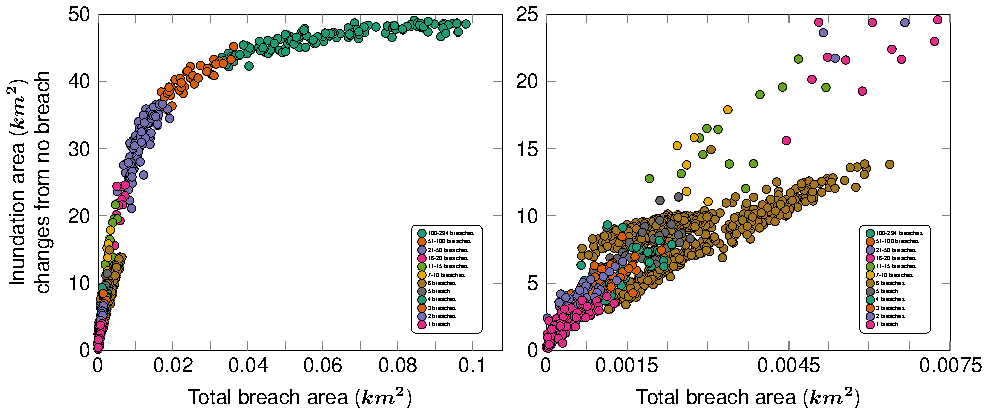
\includegraphics[width=\textwidth]{figures/fig5.pdf}
    \caption{a) Total inundation vs. total breach size for all 1500 scenarios, points are colored per number of breach categories. b) zoom in of a) panel to show differentiation of breach area and number of breaches and how the inundation can vary}
    \label{fig:5}
\end{figure}

Figure \ref{fig:7} illustrates different inundation and flooding patterns in the bay. In each case the highest flooding and inundation occurs in the low lying coastal regions and along the river entrances. The maximum surge is highest where the Forge River mouth is and as it approaches the bay the surge height decreases gradually. The creeks and rivers that drain into Seatuck Cove on the eastern side of the bay also have higher surge levels. Surge height is also higher in areas directly adjacent to a breach or the inlet and areas where there is no ready egress from the bay.


\section{Discussion}
The results of this study illustrate that location, size, and number of breaches have an impact on coastal flooding. There is a clear relationship between total breach area and the amount of flooding in the bay and on the mainland coastline. The histograms plotted in Figure \ref{fig:3} illustrate a few different sections of the bay. The west surge point located near the Forge River mouth shows that given the original breaching locations the surge distribution is clustered and overlaps across scenarios, but when the simulations are allowed to vary breach locations the maximum surge is much higher from breaches located nearby. This location is also more prone to higher surge because of the water flooding into Moriches Bay from the connection to Great South Bay. As the storm made landfall on the western edge of Great South Bay the surge is pushed from southwest to northeast.
The central location is adjacent to the mainland coastline near Seatuck Cove. Varying the breach locations and number of breaches increases the surge but to a smaller degree than in the west with the maximum surge at this location lower than in the west most likely due to proximity of the inlet which allows the water to flow out of the bay as it travels towards this location. Additionally the shape of the coastline protects this location to some extent from surge coming from the southwest. 
The east location which is closest to the barrier island has the smallest maximum surge in the bay. While surge coming from breaches on the eastern portion of the brings it a higher water level than the original breach locations the proximity to the inlet allows water from the west to flow outward back into the ocean relieving the bay side flooding during later times in the storm.

The gauges distributed in each section of the bay illustrate differences of surge timing and maximum surge. Figure \ref{fig:3} as the water moves from Great South Bay to the southwest into Moriches it is apparent that the surge is both larger and arrives earlier for the vary everything simulations. As the central gauges are reaches while the surge is still larger the timing is more in sync with the vary width, depth, both scenarios. The eastern gauges maximum surge for these locations is not much higher than the other categories of simulations however the surge does still arrive earlier coming because of more connections to the ocean.

In Figure \ref{fig:5}a we show that the total breach dimensions have a relationship to the total area of inundation, with larger and more numerous breaches bringing more water inland. Total breach area across all breaches is the strongest predictor of greater coastal inundation, until the island is significantly eroded, then inundation growth slows considerably.
Figure \ref{fig:5}b brings more nuance to this relationship. While there appears to be a stronger correlation between breach width and inundation, than depth and inundation, the impact of breach depth is at least a factor of 20 smaller than total width for these scenarios. The cluster of breaches that hover above the main grouping are the depth scenarios, whereas the width scenarios are more linear.

\begin{figure}
    \centering
    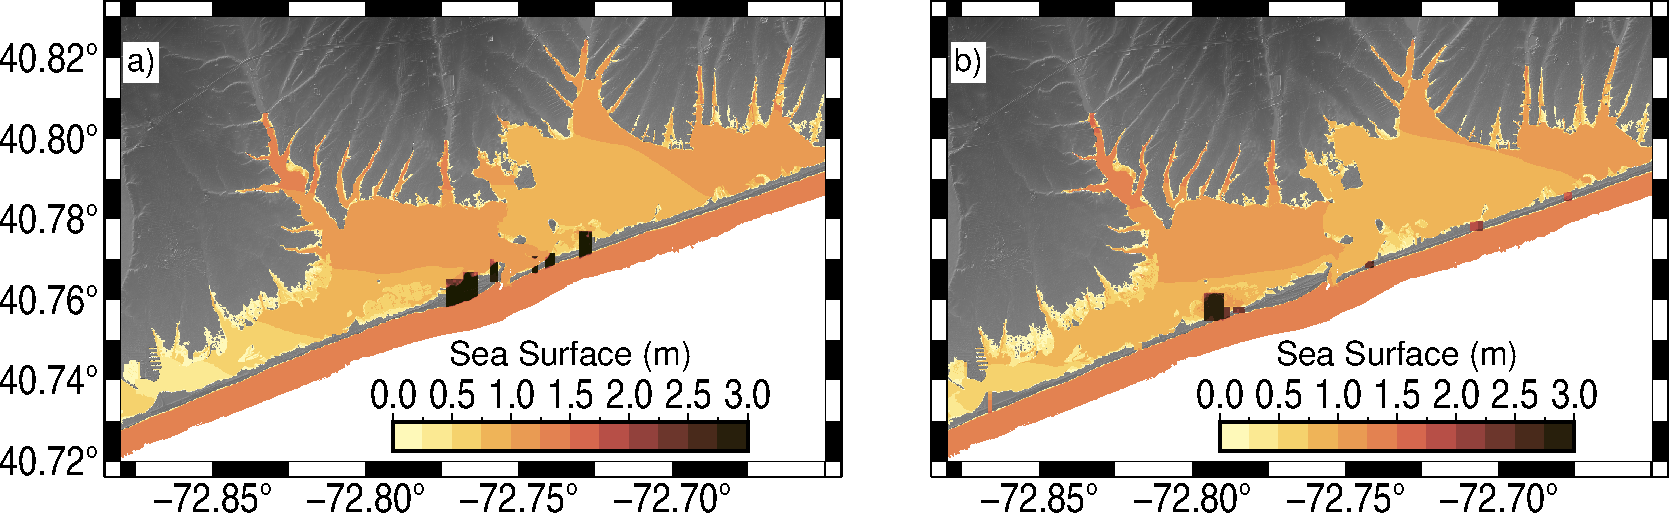
\includegraphics[width=0.95\textwidth]{figures/fig6.pdf}

    \caption{Maps Moriches Bay, NY. Each panel is a separate simulation representing different values of storm surge inundation. Panel (a) is no breach scenario. Panel (b) is the minimum inundation with a single small breach. Panel (c) is the largest inundation scenario with 6 wide breaches. Panel (d)  is a simulation that has the closest inundation to the mean of all 1500 simulations, with 4 moderate sized breaches.}
    \label{fig:6}
\end{figure}

Figure \ref{fig:6} illustrates that different inundation and bay surge patterns are correlated to number and size of breaches. Figure \ref{fig:6} panel a) is a no breach scenario which looks very similar in surge and inundation distribution to the minimum inundation (panel b) which has only a single small breach. There are approximately 500 different wet vs. dry cells between these two simulations, which is 163,200 square meters or .1632 square kilometers of inundation. Figure \ref{fig:6} panel d) is a simulation that comes closest to the mean of all the inundation change from all 1500 simulations. There are six medium to large sized breaches with a total breach area of .005 $km^2$ and total inundation change of 13.06 $km^2$. The shape of the highs and lows of bay flooding and coastal inundation is very different from the no breach or minimum inundation scenarios, with higher flooding potential in the coves, creeks and rivers that border the bay and along the lower elevation coastlines. Lastly the maximum inundation scenario is one where most of the island has been breached, this scenario has a bay surge of approximately two meters in most areas and the lowest elevation areas of the coastline are completely flooded.

The impact differing breach locations has on inundation as illustrated in Figure \ref{fig:6}b, can be further seen in Figure \ref{fig:7}. This figure shows the differences between two simulations with a similar total breach area, however the total inundation is very different. Figure \ref{fig:6}a, shows a scenario with six moderately sized breaches in the locations that occurred during the 1938 hurricane, the total breach area is .0039 $km^2$, and total inundation is 10.44 $km^2$. Figure \ref{fig:6}b, has a smaller total breach area of .0036 $km^2$ but a larger inundation at 12.03 $km^2$. The breaches in this scenario are generally smaller but more spaced out across the barrier island, with several in the western portion of the barrier island closer to Great South Bay. While the pattern of surge in the bay is similar it is visually different in the shape of the surge height and there is more coastal inundation along the western coastline. The Forge River surge is higher in Figure \ref{fig:6}b and the inlet region has a lower total water depth. The eastern portion of the bay has less inundation in \ref{fig:6}b, most likely due to the majority of the breaches being towards the west, plus the inlet allowing water to flow out of the bay.


\begin{figure}
    \centering
    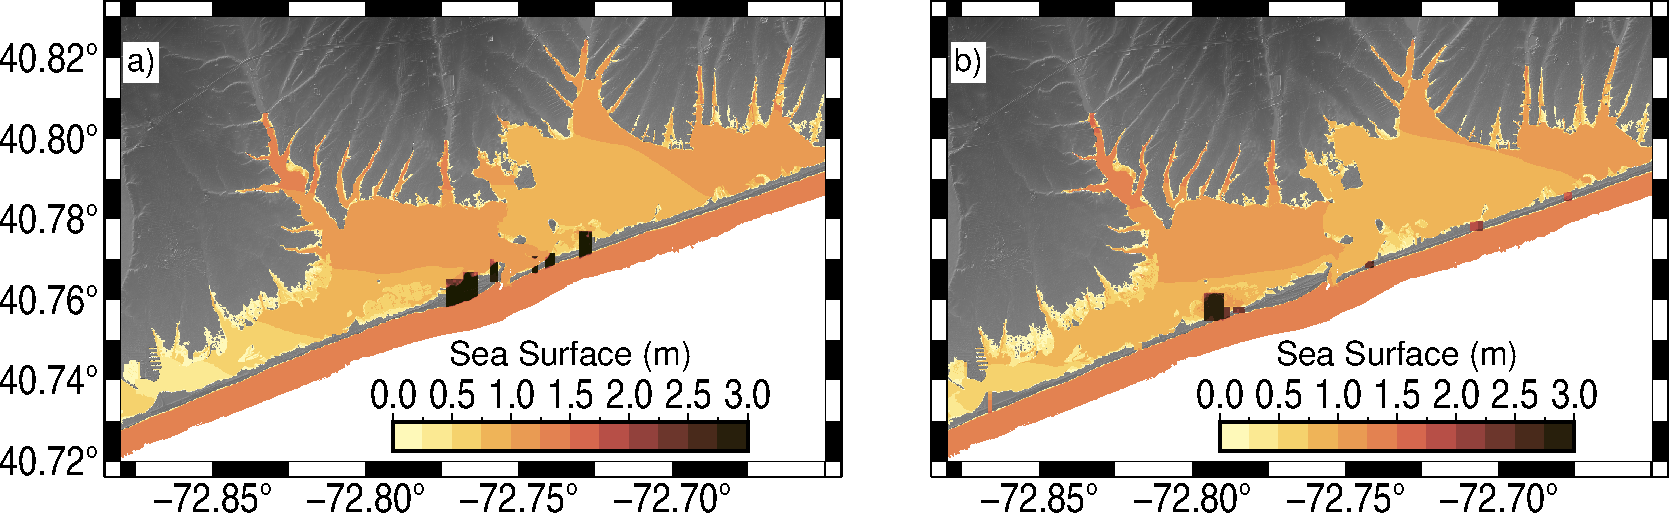
\includegraphics[width=0.95\textwidth]{figures/fig6.pdf}
    \caption{a) maximum surge and inundation for simulation that has 11 breaches and a total area of 0.036 $km^2$. b) maximum surge and inundation for simulations with 6 breaches and .039 $km^2$}
    \label{fig:7}
\end{figure}

Figures \ref{fig:6} and \ref{fig:7} highlight the important details we discovered across our different simulations. Total breach area is a very strong predictor of total inundation. However, location of breaching is also very important, especially given the dynamics of the storm forcing and direction with which the surge is being pushed.

\section{Conclusions}
Breaching of a barrier island during a hurricane shows a strong impact on mainland inundation. The number, locations, and size of the breaches can change the inundation potential for the coastline. Understanding vulnerable areas and how breaching impacts them can provide opportunities for shoring up infrastructure and allowing planning that minimizes the storm's disruption to lives and the community.
Future work that can expand this study. Run many more simulations to find a better statistical distribution of the different breaching simulations. It will take a lot more data to find a consensus on specifically vulnerable locations, patterns of breaching, and its coastal impacts. Repeating simulations but varying the storms, will also provide insight into how the approach, speed, landfall location, and size of the storm affects the flooding and inundation.


\bibliography{ref}

\end{document}
